\documentclass{report}
% Maths Packages
\usepackage{mathtools, amsthm, amssymb, mathrsfs, interval, stmaryrd, centernot, esvect, cancel, commath, blkarray, empheq}
\usepackage{tabularx}
\usepackage{booktabs}
\usepackage{cellspace}
\setlength{\cellspacetoplimit}{5pt}
\setlength{\cellspacebottomlimit}{5pt}


% Sagemaths Formating Packages
\usepackage{listings}
\lstdefinelanguage{Sage}[]{Python}
{morekeywords={False,sage,True},sensitive=true}
\lstset{
  frame=none,
  showtabs=False,
  showspaces=False,
  showstringspaces=False,
  commentstyle={\ttfamily\color{dgreencolor}},
  keywordstyle={\ttfamily\color{dbluecolor}\bfseries},
  stringstyle={\ttfamily\color{dgraycolor}\bfseries},
  language=Sage,
  basicstyle={\fontsize{10pt}{10pt}\ttfamily},
  aboveskip=0.4em,
  belowskip=0.4em,
}

% TOC Packages
\usepackage{tocloft, titletoc, hyperref, bookmark}
% Formatting / Style Packages
\usepackage[T1]{fontenc}
\usepackage{geometry, subcaption, graphicx, fix-cm, accents, float, varwidth, soul, ulem, contour, multicol, enumitem}    
\usepackage[bottom]{footmisc}
\usepackage[x11names, table]{xcolor}
\usepackage[most, skins]{tcolorbox}
\usepackage{adjustbox}
\DeclareMathAlphabet{\mathmybb}{U}{bbold}{m}{n} % Indicatrices
\newcommand{\1}{\mathmybb{1}}

% Tikz
\usepackage{tikz, tkz-fct, tkz-euclide, tikz-cd, tkz-fct, pgfplots}
\pgfplotsset{compat=1.18}
\usetikzlibrary{
  angles, quotes, 3d, positioning,
  shapes,fit, arrows, arrows.meta, calc, 
  matrix, calligraphy, intersections, 
  quotes, patterns, patterns.meta, 
  decorations.pathreplacing, decorations.markings,decorations.pathmorphing,
}
\usepgfplotslibrary{fillbetween}
\tikzset{
  withparens/.style = {draw, outer sep=0pt,
    left delimiter= (, right delimiter=),
    above delimiter= (, below delimiter=),
    align=center},
  withbraces/.style = {draw, outer sep=0pt,
    left delimiter=\{, right delimiter=\},
    above delimiter=\{, below delimiter=\},
    align=center}
}
\tikzcdset{
  arrow style=tikz,
  diagrams={>={Straight Barb[scale=1]}},
}

% PAGE SETTINGS

\geometry{
  left=25mm, right=25mm, top= 15mm, bottom= 15mm,
  footskip=30pt
  }
\setlength{\parindent}{0cm}
\setlength{\parskip}{0cm}
\setlist[itemize]{itemsep=0pt, leftmargin=25pt}

\setlength{\cftbeforetoctitleskip}{0pt}
\setlength{\cftaftertoctitleskip}{0pt}

\setcounter{secnumdepth}{-1}

% STYLE
\definecolor{BrightBlue1}{RGB}{95, 150, 210}

\definecolor{BrightRed1}{RGB}{210, 95, 95}
\definecolor{BrightRed2}{RGB}{210, 115, 115}

\definecolor{DarkBlueX}{RGB}{43, 68, 92}
\definecolor{DarkBlue0}{RGB}{53, 78, 102}
\definecolor{DarkBlue1}{RGB}{83, 108, 132}
\definecolor{DarkBlue2}{RGB}{58, 94, 132}
\definecolor{DarkBlue3}{RGB}{90, 126, 162}

\definecolor{DarkGreen3}{RGB}{83, 132, 108}
\definecolor{DarkGreen2}{RGB}{58, 132, 94}
\definecolor{DarkGreen1}{RGB}{90, 162, 126}
\tcbset{shield externalize, enhanced, sharp corners, halign=center, center}

\definecolor{dblackcolor}{rgb}{0.0,0.0,0.0}
\definecolor{dbluecolor}{rgb}{0.01,0.02,0.7}
\definecolor{dgreencolor}{rgb}{0.2,0.4,0.0}
\definecolor{dgraycolor}{rgb}{0.30,0.3,0.30}
\newcommand{\dblue}{\color{dbluecolor}\bf}
\newcommand{\dred}{\color{dredcolor}\bf}
\newcommand{\dblack}{\color{dblackcolor}\bf}

%Underline settings
\setlength{\ULdepth}{2pt}
\contourlength{0.8pt}
\renewcommand{\underline}[1]{
  \uline{\phantom{#1}}%
  \llap{\contour{white}{#1}}%
}

%drop shadow southwest=black!100!black
\newcommand{\secstyle}[1]{\color{DarkBlue1}\fbox{#1}}
\newcommand{\subsecstyle}[1]{\color{DarkBlue2}\underline{#1}}
\newcommand{\subsubsecstyle}[2]{\color{DarkBlue3}\underline{#1}}

\newcommand{\chapterstyle}[1]{
    \setlength{\fboxsep}{0.3em}
    \setlength{\fboxrule}{3pt}
    \centering\vspace{-70pt}
    
    \color{DarkBlue1}\huge\fbox{\textbf{\textsc{#1}}}
}

\newcommand{\customBox}[2]{
    \tcbset{boxrule=1.5pt, boxsep=-0.2mm, colframe=DarkBlue1, colback=BrightBlue1!05}
    \begin{tcolorbox}[#1]
        \abovedisplayskip=0pt % remove vertical space above align
        #2
    \end{tcolorbox}
}

\makeatletter % Crée une trés grosse taille de police pour la page de garde
\newcommand\HUGE{\@setfontsize\Huge{40}{60}}
\makeatother   

\makeatletter
\newcommand\footnoteref[1]{\protected@xdef\@thefnmark{\ref{#1}}\@footnotemark}
\makeatother

% COMMANDS
% TOC
\renewcommand{\cftchapfont}{\large \bfseries \scshape}
\renewcommand{\cftsecfont}{}
\renewcommand{\contentsname}{\hfill
\setlength{\fboxsep}{0.3em}\setlength{\fboxrule}{3pt}\vspace{20pt}
   \color{DarkBlue1}\Huge
   \fbox{\textbf{\textsc{Table des matières}}}
   \hfill
}

% MATHS
\newcommand{\C}{\mathbb{C}}
\newcommand{\R}{\mathbb{R}}
\newcommand{\Q}{\mathbb{Q}}
\newcommand{\Z}{\mathbb{Z}}
\newcommand{\N}{\mathbb{N}}
\newcommand{\U}{\mathbb{U}}
\newcommand{\K}{\mathbb{K}}

\newcommand{\A}{\mathbf{\mathscr{A}}}
\newcommand{\B}{\mathbf{\mathscr{B}}}
\newcommand{\Fam}{\mathbf{\mathscr{F}}}
\renewcommand{\P}{\mathbf{\mathscr{P}}}

\renewcommand{\epsilon}{\varepsilon}
\renewcommand{\rho}{\varrho}

\newcommand{\E}{\mathbf{\mathcal{E}}}
\newcommand{\F}{\mathbf{\mathcal{F}}}
\newcommand{\Pow}{\mathbf{\mathcal{P}}}
\newcommand{\G}{\mathbf{\mathfrak{G}}}

\newcommand{\<}{\bigskip}
\newcommand{\+}{\par}

% Notation equality

\newcommand\notationEq{\stackrel{\mbox{
    \begin{tiny}  
        notation
    \end{tiny}    
}}{=}}

% INTERVALS

\intervalconfig{separator symbol =  \,; \,}

\newcommand{\ioo}[2]{\interval[open]{#1}{#2}}
\newcommand{\ioc}[2]{\interval[open left]{#1}{#2}}
\newcommand{\ico}[2]{\interval[open right]{#1}{#2}}
\newcommand{\icc}[2]{\interval{#1}{#2}}

\newcommand{\intioo}[2]{\left\rrbracket{#1}\;;\;{#2}\right\llbracket}
\newcommand{\intioc}[2]{\left\rrbracket{#1}\;;\;{#2}\right\rrbracket}
\newcommand{\intico}[2]{\left\llbracket{#1}\;;\;{#2}\right\llbracket}
\newcommand{\inticc}[2]{\left\llbracket{#1}\;;\;{#2}\right\rrbracket}

% EQUATIONS NOTES

\newcommand{\shorteqnote}[1]{ &  & \text{\small\llap{#1}}}
\newcommand{\longeqnote}[1]{& & \\ \notag&  &  &  &  & \text{\small\llap{#1}}}

% FUNCTIONS NOTATIONS

\newcommand{\inject}{\hookrightarrow} 
\newcommand{\surject}{\twoheadrightarrow}

% MOD NOTATION

\newcommand{\eqmod}[1]{\underset{#1}{\equiv}} 

% LINEAR ALGEBRA

\newcommand{\dotproduct}[2]{\left\langle\;\! #1 \;\! | \;\! #2 \;\! \right\rangle}
\newcommand{\vectNorm}[1]{\left\Vert#1 \right\Vert}

\newcommand{\Ker}[1]{\text{Ker}#1}
\newcommand{\Sp}[1]{\text{Sp}(#1)}
\renewcommand{\Im}[1]{\text{Im}#1}

\NewDocumentCommand{\opNorm}{sO{}m}{%
  \IfBooleanTF{#1}{% automatic scaling, use with care
    \left|\opnormkern\left|\opnormkern\left|
    #3
    \right|\opnormkern\right|\opnormkern\right|
  }{
    \mathopen{#2|\opnormkern #2|\opnormkern #2|}
    #3
    \mathclose{#2|\opnormkern #2|\opnormkern #2|}
  }%
}
\newcommand{\opnormkern}{\mkern-1.5mu\relax}% adjust for the font

% TOPOLOGY
\newcommand{\ball}{\mathscr{B}}

% CALCULUS
\newcommand{\partialD}[2]{\frac{\partial #1}{\partial #2}}

% GEOMETRY
\newcommand{\RightAgnle}[4][5pt]
{%
    \draw($#3!#1!#2$)-- ($#3!2! ($ ($#3!#1!#2$)!.5! ($#3!#1!#4$)$)$)-- ($#3!#1!#4$);
}

% PROBABILITIES
\newcommand{\probability}[1]{\mathbb{E} (#1)}
\newcommand{\expectancy}[1]{\mathbb{E} (#1)}
\newcommand{\variance}[1]{\mathbb{V} (#1)}
\newcommand{\covariance}[1]{\mathbb{C} (#1)}



\begin{document}
   \begin{titlepage}
   \begin{center}
       \vspace*{1cm}
       {
           \hfill
           \setlength{\fboxsep}{0.8em}\setlength{\fboxrule}{4pt}
           \color{DarkBlue1}\HUGE\fbox{\textbf{\textsc{Mathématiques}}}\hfill}

       \<
       {
       \color{DarkBlue1}\Large
       \textsc{Master}
       }
       \<

       \vspace{1.5cm}

       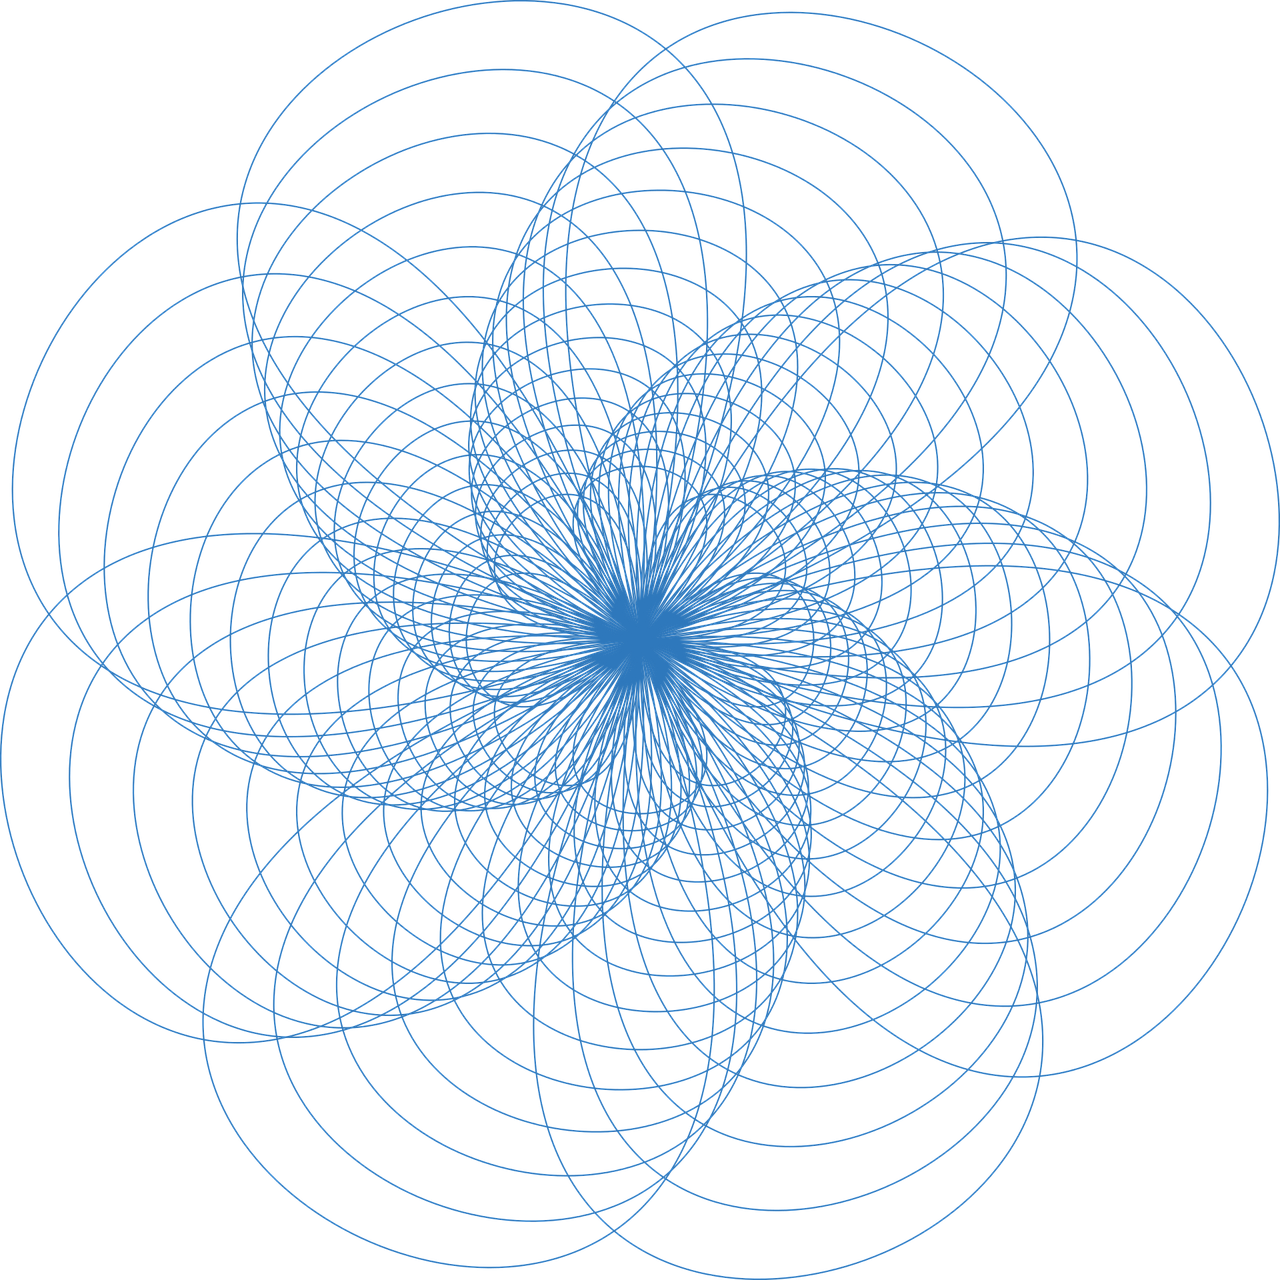
\includegraphics[width=0.9\textwidth]{Cover.png}

       \vfill

       \large
       \textsc{Université Paul Sabatier}\\
       \textsc{Année 2025-2027}
   \end{center}
\end{titlepage}

   \renewcommand{\cftchapfont}{\large \bfseries \scshape}
   \renewcommand{\cftsecfont}{}
   \renewcommand{\contentsname}{\hfill
   \setlength{\fboxsep}{0.3em}\setlength{\fboxrule}{3pt}\vspace{20pt}
   \color{DarkBlue1}\Huge
   \fbox{\textbf{\textsc{Table des matières}}}
   \hfill
   }
   
   \setcounter{tocdepth}{1}
   \tableofcontents

   \addcontentsline{toc}{chapter}{Fondements} % 95%
   \chapter*{\chapterstyle{I --- Raisonnements}}
\addcontentsline{toc}{section}{Raisonnements}

Soit \(\P\) une proposition et \(n\) un entier naturel.

\subsection*{\subsecstyle{Disjonctions \& Conjonctions {:}}}
\addcontentsline{toc}{subsection}{Disjonctions \& Conjonctions}

Si \(\P\) est une disjonction de la forme \(\A \lor \B\), il suffit alors de supposer \textbf{l'une des deux propriétés fausse} et de montrer que l'autre est vraie.\<

Si \(\P\) est une conjonction de la forme \(\A \land \B\), il faut simplement prouver \(\A\) et \(\B\).

\subsection*{\subsecstyle{Raisonnements par l'absurde {:}}}
\addcontentsline{toc}{subsection}{Raisonnements par l'absurde}

Raisonner par l'absurde revient à utiliser le principe du \textbf{tiers exclu}, ie l'axiome qui affirme que la proposition ci-dessous est toujours vraie:
\[
   \P \, \lor \, \lnot \P
\]
Donc si on veut prouver \(\P\), on peut alors simplement montrer que \(\lnot\P \implies \bot\) avec ''\(\bot\)'' comme notation d'une contradiction logique. Alors on peut conclure d'après l'axiome du tiers exclu que \(\P\) est vraie. 

\subsection*{\subsecstyle{Raisonnement par Analyse / Synthèse {:}}}
\addcontentsline{toc}{subsection}{Raisonnements par Analyse / Synthèse}

Le raisonnement par Analyse / Synthèse permet de déterminer \textbf{l'ensemble des solutions d'un problème}, il s'effectue en deux étapes, tout d'abord l'étape d'analyse suppose qu'une telle solution existe, alors on circonscrit son existence à des propriétés connues qu'elle vérifie nécessairement. Cette étape permet de ''cerner'' les solutions en question. Si les propriétés sont assez contraignantes, alors on peut même prouver \textbf{l'unicité}, ie l'ensemble des solutions se réduit à un singleton.\<

Puis lors de l'étape de synthèse, on considère un objet vérifiant les propriétés qu'on a utilisé lors de l'étape d'analyse, et on \textbf{vérifie} que cet objet est bien une solution au problème initial. C'est lors de cette étape qu'on prouve bien \textbf{l'existence} de solutions. Si aucun des objets circonscrits par l'analyse ne conviennent, le problème n'a alors pas de solutions.

\subsection*{\subsecstyle{Implications \& Équivalences {:}}}
\addcontentsline{toc}{subsection}{Implications \& Équivalences}

Si \(\P\) est une implication de la forme \(\A \implies \B\), on a les équivalences suivantes:
\[
   \P \Longleftrightarrow \lnot \A \lor \B \Longleftrightarrow \lnot \B \implies \lnot \A
\]
Aussi en raisonnant \textbf{par l'absurde}, il suffit alors de prouver:
\[
   \A \land \lnot \B \implies \bot 
\]
Il est important de noter que l'implication \textbf{n'est pas une opération associative}, en effet, soit une propriété de la forme:
\[
   \A_1 \implies \A_2 \implies \A_3
\]
Alors de manière générale, on a:
\[
   \A_1 \implies (\A_2 \implies \A_3) \centernot\Longleftrightarrow (\A_1 \implies \A_2) \implies \A_3
\]
Prouver une équivalence revient à prouver une \textbf{double implication} dans la majorité des cas.\<

\underline{Cas particulier {:}}
Si \(\P\) est de la forme \( A_1 \Longleftrightarrow A_2 \Longleftrightarrow \cdots \Longleftrightarrow \A_{n-1} \Longleftrightarrow \A_n \), il suffit alors de montrer:
\[
   \A_1 \implies \A_2 \implies \cdots \implies \A_{n-1} \implies \A_n \implies \A_1
\]
Ainsi pour toute paire de \(\A_i\), on a bien double implication entre les deux membres et donc la chaîne d'équivalence est démontrée.

\subsection*{\subsecstyle{Raisonnements par récurrence {:}}}
\addcontentsline{toc}{subsection}{Raisonnements par récurrence}

Soit \(\P\) une propriété dépendante de \(n\) qu'on veut démontrer sur \(\inticc{\alpha}{+\infty}\), soit \(k\) en entier fixé supérieur à \(\alpha\), démontrer \(\P\) par récurrence simple revient à utiliser \textbf{l'axiome de récurrence} (issu de la construction de \(\N\)) ci-dessous:
\[
   \Bigr[ \P_{\alpha} \; \land \; \bigr[ \P_{k} \implies \P_{k+1} \bigr] \Bigr] \implies \forall n \in \N \; ; \; \P_n   
\]

Si la propriété à prouver est plus complexe, on peut avoir besoin de récurrences d'une autre type, en effet si \(\P\) dépend \textbf{des deux rangs précédents}, et on utilise alors une récurrence à deux pas qui s'exprime:
\[
   \Bigr[ \P_{\alpha} \; \land \; \P_{\alpha + 1} \; \land \; \bigr[ \P_{k-1}  \land \P_{k}\implies \P_{k+1} \bigr] \Bigr] \implies \forall n \in \N \; ; \; \P_n   
\]

Enfin pour le cas limite, si \(\P\) dépends \textbf{d'exactement tout les rangs précédents}, alors on peut utiliser une récurrence forte qui s'exprime:
\[
   \Bigr[ \P_{\alpha} \; \land \bigr[ \P_{\alpha + 1} \; \land \; \ldots \; \P_{k-1} \; \land \; \P_{k} \implies \P_{k+1}  \bigr] \Bigr] \implies \forall n \in \N \; ; \; \P_n   
\]
Un dernier type de récurrence appelé \textbf{récurrence limitée} permet simplement d'utiliser la récurrence sur un intervalle entier fini, et donc on initialise et on prouve l'hérédité avec la contrainte de cette intervalle.\<


\underline{Remarque sur la récurrence forte {:}}\<

Une telle récurrence forte ne nécessitera qu'une \textbf{unique} initialisation pour compléter l'hérédité.\<

D'un point de vue heuristique, il peut arriver d'engager une récurrence forte sur un problème qui n'aurait nécessité qu'une récurrence à \(p\) pas.\+
Ce cas précis reviendra alors, lors de l'étape d'hérédité, à \textbf{ne pas utiliser l'ensemble de l'hypothèse de récurrence}, et alors il faudra modifier le nombre d'initialisation à réaliser et l'intervalle de notre hypothèse de récurrence.\<

Admettons que \(\P_\alpha\) soit vraie, supposons qu'elle soit vraie sur \(\inticc{\alpha}{k}\). Alors, on doit montrer que la propriété est vraie au rang \(k + 1\).\<

Alors, selon \textbf{le plus petit rang} nécessaire à compléter l'hérédité, on a:
\begin{align*}
    & \text{Si on a besoin de } \P_k \text{ alors \textbf{on se ramène à une récurrence simple.}}\\
    & \text{Si on a besoin de } \P_{k-1} \text{ alors \textbf{on se ramène à une récurrence double.}}\\
    & \text{Si on a besoin de } \P_{k-2} \text{ alors \textbf{on se ramène à une récurrence triple.}}\\
    & \ldots\ldots\ldots
\end{align*}
Et donc, les initialisations et l'intervalle de notre hypothèse de récurrence changeront en conséquence et on remarque alors que si le plus petit rang nécessaire est \(\P_{k-p}\), alors on se ramène nécessairement à une \textbf{récurrence à \(p\) pas}, avec \(p\) initialisations et l'hypothèse de récurrence qui commence à \(\alpha + p\).\<

Une récurrence forte n'est alors qu'une récurrence qui nécessite des hypothèses sur \textbf{tout les rangs précédents.}
   
\subsection*{\subsecstyle{Récurrences imbriquées {:}}}
\addcontentsline{toc}{subsection}{Récurrences imbriquées}

Soit \(\P_{n,m}\) une propriété qui dépend \textbf{de deux variables entières}, alors on pourrait prouver \(\P_{n, 0}\) par récurrence et alors cela constituerait l'initialisation d'une récurrence imbriquée qui supposerait par exemple \(\P_{n, k}\) vraie pour prouver \(\P_{n, k+1}\).
\chapter*{\chapterstyle{I --- Ensembles}}
\addcontentsline{toc}{section}{Ensembles}

Soit \(E\), \(F\) et \(X\) trois ensembles quelconques.
On note tout d'abord que l'intersection est prioritaire sur la réunion lors d'opérations sur les ensembles et que les deux opérations sont \textbf{distributives} l'une par rapport à l'autre.

\subsection*{\subsecstyle{Inclusion {:}}}
\addcontentsline{toc}{subsection}{Inclusion}

L'inclusion est une \textbf{relation d'ordre} sur l'ensemble des parties de \(E\), et donc on en déduit qu'elle est \textbf{réflexive, transitive et antisymétrique}. Si l'inclusion est stricte, on parle de \textbf{sous-ensemble propre}.\<

Si \(E \subseteq F\), on a:
\begin{flalign*}
    E \cap F = E\\
    E \cup F = F
\end{flalign*}
Aussi, les opérations élémentaires préservent l'inclusion:

\customBox{width=4cm}{
    \begin{align*}
        E \cap X \subseteq F \cap X \\
        E \cup X \subseteq F \cup X
    \end{align*}
}


\subsection*{\subsecstyle{Complémentaire et de la différence {:}}}
\addcontentsline{toc}{subsection}{Complémentaire et différence}


Si \(F \subseteq E\), alors \(F^c\) est l'ensemble qui contient tout les éléments de \(E\) qui \textbf{ne sont pas} dans \(F\) et on a définit alors \textbf{la différence ensembliste}:
\[
   E \;\backslash\; F = E \cap F^c  
\]
Par ailleurs, \textbf{les lois de De Morgan} nous donnent:
\customBox{width=4cm}{
    \begin{align*}
        (E \cap F)^c = E^c \cup F^c \\
        (E \cup F)^c = E^c \cap F^c
    \end{align*}
}
\underline{Cas particulier {:}}
On peut aussi définir l'opération de \textbf{différence symétrique} notée \(\Delta\) qui permet d'obtenir tout les éléments qui appartiennent exactement à un seul des deux ensembles:
\[
   E \Delta F = (E \cup F) \;\backslash\; (E \cap F)   
\]

\subsection*{\subsecstyle{Produit cartésien {:}}}
\addcontentsline{toc}{subsection}{Produit cartésien}

Soit \(n\) une entier naturel, le produit cartésien des ensembles \(E_1,\, E_2,\, \ldots\,,\, E_{n-1},\, E_n\) est l'ensemble des n-uplets de la forme (\(e_1, e_2, \ldots, e_{n-1}, e_n\)) avec \(e_i \in E_i\) pour \(i \in \inticc{1}{n}\).
Il y a \textbf{unicité} de ces n-uplets.

Plus formellement, on note:
\[
     \prod_{i=1}^{n} E_i = \Bigl\{ (e_1, e_2, \ldots, e_{n-1}, e_n) \; ; \; e_1 \in E_1, e_2 \in E_2, \ldots,  e_n \in E_n \Bigl\}
\]
\pagebreak

\subsection*{\subsecstyle{Cardinalité {:}}}
\addcontentsline{toc}{subsection}{Cardinalité}

Supposons que \(E\) et \(F\) tout deux inclus dans \(X\) et ayant \textbf{un nombre fini d'éléments}. On a alors différentes propriétés:
\customBox{width=6cm}{
    \begin{align*}
        |E \cup F| &= |E| + |F| - |E \cap F| \\
        |E \times F| &= |E| \times |F| \\
        |E^c| &= |X| - |E| \\
        |\Pow_E| &= 2^{|E|}
    \end{align*}
}
\subsection*{\subsecstyle{Partitions et recouvrements{:}}}
\addcontentsline{toc}{subsection}{Partitions et recouvrements}

Soit \((P_i)_{i \in \N}\) une famille de parties \textbf{non vides et deux à deux disjointes} de \(E\).\+
On dit que \((P_i)\) est une \textbf{partition} de E si et seulement si:
\[
    \bigcup_{i \in \N} P_i = E
\]
On remarque immédiatement deux partitions singulières:
\begin{align*}
    &\bullet \text{ La famille contenant uniquement } E \text{ qu'on appelle \textbf{partition grossière}.} \\
    &\bullet \text{ La famille contenant tout les singletons de } E \text{ qui est la partition \textbf{la plus fine}.}
\end{align*}
On peut donc intuitivement parler de \textbf{finesse} d'une partition, en regard de la taille des parties de la famille.\<

On peut généraliser le concept de partitition à celui de \textbf{recouvrement}, alors \(E\) ne nécessite que d'être contenu par l'union des \((P_i)\).

\subsection*{\subsecstyle{Algèbre de Boole {:}}}
\addcontentsline{toc}{subsection}{Algèbre de Boole}

On peut montrer que l'ensemble \textbf{ordonné} des parties de \(E\) muni de l'union, l'intersection, le complémentaires forment une \textbf{Algèbre de Boole}.\<

Cela signifie que la structure \((\Pow(E), \cup, \cap, X^c)\) vérifie les axiomes suivants:
\begin{align*}
    &\bullet \text{ Les deux opérations binaires sont \textbf{associatives, commutatives et distributives l'une sur l'autre.}}\\
    &\bullet \text{ Les deux opérations binaires sont \textbf{idempotentes.}}\\
    &\bullet \text{ \textbf{L'élément neutre} pour l'union est l'ensemble vide, et pour l'intersection l'ensemble \(E\).}\\
    &\bullet \text{ \textbf{L'élément absorbant} pour l'union est l'ensemble \(E\), et pour l'intersection l'ensemble vide.}\\
    &\\
    &\bullet \text{ Le complémentaire est \textbf{involutif}.}\\
    &\bullet \text{ L'intersection d'un élément et de son complémentaire est \textbf{vide}.}\\
    &\bullet \text{ L'union d'un élément et de son complémentaire est \textbf{l'ensemble tout entier}.}\\
    &\bullet \text{ Les \textbf{lois de De Morgan} sont vérifiées.}\\
\end{align*}
De manière analogue, en considérant \(\{0, 1\}\) comme les valeurs de vérité d'une proposition, on a:

\customBox{width=11cm}{
    \begin{align*}
        \textbf{La structure } (\{0, 1\}, \lor, \land, \lnot) \textbf{ est aussi une algèbre de Boole.}
    \end{align*}
}

Cette structure est à la base de la logique formelle et vérifie les même axiomes que l'algèbre de l'ensemble des parties d'un ensemble.
\chapter*{\chapterstyle{I --- Relations}}
\addcontentsline{toc}{section}{Relations}

Une \textbf{relation} entre des objets d'un ensemble est une propriété que vérifient ces objets \textbf{entre eux}.\+
Les relations sont des objets \textbf{fondamentaux} en mathématiques, elles sont entre autres des objets primitifs de la théorie des ensembles.\<

On appelle \textbf{arité} le nombre d'éléments mis en jeu par la relation.\+ Par exemple une relation d'arité 2 est appelée \textbf{relation binaire} et met en jeu deux éléments. On définit ainsi le cas général de relation \textbf{n-aire} qui met en jeu \(n\) éléments \(x_1, x_2, \ldots, x_{n-1}, x_n\) et on note:
\[
    \mathscr{R}(x_1, x_2, \ldots, x_{n-1}, x_n)
\]
\textbf{Par abus de langage}, on appelle \textbf{classe} un ensemble d'ensembles.\+
Formellement une classe n'est pas un ensemble mais un élément primitif de la théorie ZFC, mais ici on verra qu'on appelle classe des objets qui \textbf{sont} des ensembles.

\subsection*{\subsecstyle{Zoologie {:}}}
\addcontentsline{toc}{subsection}{Zoologie}

Il existe un grand nombre de relations très connues et élémentaires, par exemple:
\begin{align*}
    &\bullet \text{ La relation d'appartenance à un ensemble} \\
    &\bullet \text{ La relation d'égalité} \\
    &\bullet \text{ La relation d'ordre} \\
    &\bullet \text{ La relation d'inclusion} \\
    &\bullet \text{ La relation de congruence} \\
    &\bullet \text{ La relation de parallélisme de deux droites du plan}
\end{align*}
On peut remarque que la relation d'appartenance à un ensemble est une relation binaire fondamentale, à la base de la théorie des ensembles.

\subsection*{\subsecstyle{Relations binaires {:}}}
\addcontentsline{toc}{subsection}{Relations binaires}

Soit \(x, y, z \in E\), une relation entre deux éléments peut vérifier plusieurs propriétés remarquables:
\[
    \begin{aligned}
        &\bullet \textbf{ Réflexivité : } \mathscr{R}(x, x)\\
        &\bullet \textbf{ Symétrie : } \mathscr{R}(x, y) \implies \mathscr{R}(y, x)\\
    \end{aligned}
    \hspace{60pt}
    \begin{aligned}
        &\bullet \textbf{ Irréflexivité : } \cancel{\mathscr{R}}(x, x)\\
        &\bullet \textbf{ Antisymétrie : } \mathscr{R}(x, y) \land \mathscr{R}(y, x) \implies x = y \\
    \end{aligned}
\]
Elle peut aussi être \textbf{transitive}:
\[
    \mathscr{R}(x, y) \land \mathscr{R}(y, z) \implies \mathscr{R}(x, z)\\
\]
On appelle aussi relation \textbf{totale} une relation telles si pour toute paire d'éléments, on a \(\mathscr{R}(x, y) \lor \mathscr{R}(y, x)\).
\pagebreak

\subsection*{\subsecstyle{Relations d'ordre {:}}}
\addcontentsline{toc}{subsection}{Relations d'ordre}

Une \textbf{relation d'ordre} est une relation \textbf{réflexive, antisymétrique et transitive}. Elle induit un ordre sur l'ensemble \(E\), qui peut potentiellement être \textbf{total}.\<

Des relations d'ordre très connues sont la relation \(\leq\) sur les ensembles de nombres ou la relation \(\subseteq\) sur l'ensemble des parties de \(E\).\<

On appelle relation de \textbf{préordre} toute relation relation d'ordre qui n'est pas antisymétrique. Intuitivement, une relation de préordre est une relation d'ordre à ``équivalence près`` des éléments.

\subsection*{\subsecstyle{Relations d'équivalence {:}}}
\addcontentsline{toc}{subsection}{Relations d'équivalence}

Une \textbf{relation d'équivalence} est une relation \textbf{réflexive, symétrique et transitive}. Intuitivement, elle met en relation les éléments des ensembles qui sont ``similaires``.\<

Des relations d'équivalence très connues sont la relation \(=\) et \(\equiv\) sur les ensembles de nombres, ou encore la relation \(\sim\) sur l'ensemble des fonctions.

\subsection*{\subsecstyle{Classes d'équivalence {:}}}
\addcontentsline{toc}{subsection}{Classes d'équivalence}

Soit \((E, \sim)\) un ensemble muni d'une relation d'équivalence.\+
Les \textbf{classes d'équivalence} de \(E\) par rapport à la relation \(\sim\) sont alors les parties de \(E\) contenant des éléments en relation.\<

Soit \(x \in E\), on définit alors la \textbf{classe d'équivalence} de \(x\) et on note \([x]\) l'ensemble:
\[
    [x] := \Bigr\{ \alpha \in E \; ; \; \alpha \sim x \Bigr\}
\]
D'après les propriété de la relation, on a alors:
\customBox{width=4cm}{
    \(x \sim y \Longleftrightarrow [x] = [y]\)
}
Et on appelle \textbf{représentant} de \([x]\) tout élément qui appartient à \([x]\).

\subsection*{\subsecstyle{Ensembles quotient {:}}}
\addcontentsline{toc}{subsection}{Ensembles quotient}

L'ensemble des classes d'équivalence de \(E\) forme alors une \textbf{partition} de \(E\), et on appelle \textbf{ensemble quotient}, ou encore \textbf{ensemble quotienté par la relation d'équivalence} l'ensemble:
\[
    E / \sim \; := \Bigr\{ [x] \in \Pow(E) \; ; \; x \in E \Bigr\}
\]
C'est alors un ensemble de classes d'équivalences par rapport à la relation \(\sim\).\<

Travailler avec l'ensemble quotient revient alors à ne pas distinguer les éléments équivalents entre eux.\+
On peut aussi créer des \textbf{structures} quotient, il suffit alors de quotienter une structure algébrique de telle sorte que les propriétés de structure soient conservées.\<

Quelques exemples connus de structures quotient:
\begin{align*}
    &\bullet \textbf{ L'anneau } \Z \,/\, n\Z := (\Z \,/\, \sim, +, \times) \textbf{ pour la relation } a \sim b \Longleftrightarrow a \equiv b [n] \\
    &\bullet \textbf{ Le corps } \Q := ((\Z \, ; \, \Z \, \backslash \, \{0\}) \, / \, \sim, +, \times) \textbf{ pour la relation } (a, b) \sim (c, d) \Longleftrightarrow ad = bc
\end{align*}
\chapter*{\chapterstyle{I --- Fonctions \& Applications}}
\addcontentsline{toc}{section}{Fonctions \& Applications}

On appelle \textbf{fonction} ou \textbf{application} des cas particulier de relation entre deux ensembles, soit \(f, g\) deux fonctions telles que:
\[
   \begin{aligned}
      f: E &\longrightarrow F\\
      x &\longmapsto f(x)
   \end{aligned}
      \hspace{50pt}
   \begin{aligned}
      g: G&\longrightarrow H\\
      x&\longmapsto g(x)
   \end{aligned}
\]

On note \(D_f\) le sous-ensemble de \(E\) tel que \(f(x)\) existe, alors \(f\) est une \textbf{application} si et seulement si \(E = D_f\) et on note alors \(\mathscr{F}(E, F)\) l'ensemble des \textbf{applications} de E vers F.\<

Si \(F \subseteq G\), alors on définit \textbf{la composée} \(g \circ f\) par la fonction \(h: x \in E \longmapsto g(f(x)) \in H\)

\subsection*{\subsecstyle{Cas des suites {:}}}
Une suite à valeurs dans \(E\) n'est alors qu'un cas particulier en la forme d'une fonction \(u : \N \longrightarrow E\), ce sont des objets d'étude trés importants en analyse et notamment en topologie. Dans le cas des suites on peut définir la notion de \textbf{suite extraite}, car si \(u_n\) est une suite dans \(E\) et \(k_n\) est \textbf{suite d'entiers croissante}, alors on définit une suite extraite de \(u_n\) par:
\[
   u \circ k : \N \longrightarrow E
\]
C'est simplement les termes de la suite \(u_n\) dont on ne choisit que les termes d'indices donnés par \(k_n\).
\subsection*{\subsecstyle{Graphe {:}}}
On définit \textbf{le graphe} de \(f\) comme suit:
\[
   G_f:= \Bigl\{ (x, f(x)) \in E \times F \; ; \; x \in E\Bigl\}   
\]
Intuitivement, c'est l'ensemble des points de l'espace d'arrivée qui sont sur la courbe de la fonction.

\subsection*{\subsecstyle{Restrictions \& Prolongements {:}}}
\addcontentsline{toc}{subsection}{Restrictions \& Prolongements}

On note \(f|_A\) la restriction de \textbf{l'ensemble de départ} de \(f\) à une partie \(A\) de \(E\).\+
On note \(f|^B\) la restriction de \textbf{l'ensemble d'arrivée} de \(f\) à une partie \(B\) de \(F\).\<

Soit \(x \in D_f\), on appelle \textbf{prolongement} de \(f\), l'application \(g\) telle que \(D_f \subset D_g\) et \(g(x) = f(x)\)

\subsection*{\subsecstyle{Image directe {:}}}
\addcontentsline{toc}{subsection}{Image directe}

On appelle \textbf{image directe} d'une partie \(A\) de \(E\) l'ensemble des images par \(f\) des éléments de \(A\), ie:
\customBox{width=5cm}{
    \(f(A) := \Bigl\{ f(x) \; ; \; x \in A \Bigl\}\)
}

L'image directe est compatible avec \textbf{certaines opérations ensemblistes}, plus précisément:
\begin{multicols}{2}
    \begin{itemize}
        \item \(f(A \cap B) = f(A) \cap f(B)\)
        \item \(f(A \cup B) \subset f(A) \cup f(B)\)
    \end{itemize}
\end{multicols}

\subsection*{\subsecstyle{Image Réciproque {:}}}
\addcontentsline{toc}{subsection}{Image Réciproque}
On appelle \textbf{image réciproque} d'une partie \(B\) de \(F\) l'ensemble des antécédents par \(f\) des éléments de \(B\), ie:
\customBox{width=6cm}{
    \(f^{-1}(B) := \Bigl\{ x \in A \; ; \; f(x) \in B \Bigl\} \)
}

L'image réciproque est compatible avec \textbf{toutes les opérations ensemblistes}, plus précisément:
\begin{multicols}{2}
    \begin{itemize}
        \item \(f^{-1}(A \cap B) = f^{-1}(A) \cap f^{-1}(B)\)
        \item \(f^{-1}(A \cup B) = f^{-1}(A) \cup f^{-1}(B)\)
    \end{itemize}
\end{multicols}

\subsection*{\subsecstyle{Injections {:}}}
\addcontentsline{toc}{subsection}{Injections}

L'application \(f\) est injective si et seulement si:
\customBox{width=8cm}{
    \(\forall x_1, x_2 \in E^2 \; ; \; f(x_1) = f(x_2) \implies x_1 = x_2 \)
}
En particulier, il suffit de montrer que l'équation \(f(x) = y\) admet \textbf{au maximum une solution dans E} pour montrer que \(f\) est injective.\+
Si \(g \circ f\) est injective alors \(f\) est nécessairement injective.\<

Si \(E\) et \(F\) sont des ensembles finis, et que \(f\) est une injection, alors on a nécessairement \(|E| \leq |F|\)

\subsection*{\subsecstyle{Surjections {:}}}
\addcontentsline{toc}{subsection}{Surjections}

L'application \(f\) est surjective si et seulement si:
\customBox{width=6cm}{
    \(\forall y \in F \; , \; \exists x \in E \; ; \; f(x) = y\)
}

En particulier, il suffit de montrer que l'équation \(f(x) = y\) admet \textbf{au moins une solution dans E} pour montrer que \(f\) est surjective.\+
Si \(g \circ f\) est surjective alors \(g\) est nécessairement surjective.\<

Si \(E\) et \(F\) sont des ensembles finis, et que \(f\) est une surjection, alors on a nécessairement \(|F| \leq |E|\)

\subsection*{\subsecstyle{Bijections {:}}}
\addcontentsline{toc}{subsection}{Bijections}

L'application \(f\) est bijective si et seulement si elle est surjective et injective.\+  
Dans ce cas, \textbf{une application réciproque} \(g\) existe et elle vérifie:
\[
    \begin{cases}
        f \circ g &= Id_F \\
        g \circ f &= Id_E
    \end{cases}
\]


Réciproquement, si il existe une application \(g\) telle que \(f\) soit inversible à gauche et à droite par \(g\), alors \(f\) est bijective.
\begin{center}
    \textit{
        Intuitivement, les bijections sont exactement \textbf{les applications inversibles à gauche et à droite} par une même application.
    }
\end{center}
Si \(f\) et \(g\) sont bijectives, alors \(f \circ g\) est bijective et \((f \circ g)^{-1} = g^{-1} \circ f^{-1}\)

\subsection*{\subsecstyle{Equipotence {:}}}
\addcontentsline{toc}{subsection}{Equipotence}

Soit \(E\) et \(F\) deux ensembles quelconques.\+
Si il existe une bijection de \(E\) vers \(F\), alors on dit que ces ensembles sont \textbf{équipotents}, et on a:
\[
    |E| = |F|
\]
Cette définition du cardinal par les bijections permet de parler de cardinal d'un ensemble dans le cas \textbf{infini}.\+
Si il existe une bijection entre \(\N\) et \(E\), on dit que \(E\) est un ensemble \textbf{dénombrable} et on note:
\[
    |E| = \aleph_0
\]
Si il existe une bijection de \(\R\) dans \(E\), alors on dit que \(E\) est un ensemble \textbf{indénombrable} et on note:
\[
    |E| = \aleph_1
\]

Il n'existerait aucun ensemble dont le cardinal se situerait entre \(\aleph_0\) et \(\aleph_1\), c'est \textbf{l'hypothèse du continu}.
\chapter*{\chapterstyle{I --- Dénombrement}} % 75% Fini
\addcontentsline{toc}{section}{Dénombrement}

Soit \(E\) un ensemble, on dit que \(E\) est \textbf{fini} si il existe une bijection de \(\inticc{1}{n}\) sur \(E\).\<

On considère maintenant que \(E\) est fini, dénombrer \(E\) consiste à déterminer sa cardinalité. Informellement il s'agit souvent de compter le nombres \textbf{d'issues possibles} d'une situation donnée, on dispose alors de trois grands modèles, les \textbf{listes}, les \textbf{arrangements} et les \textbf{combinaisons}.

\subsection*{\subsecstyle{Listes}}
On appelle \textbf{liste} à \(p\) éléments de \(E\) un p-uplet constitué d'éléments de \(E\), c'est à dire \textbf{un élément du produit cartésien} \(E^p\) on remarque alors la propriété:
\begin{center}
   \textit{
      Dans une liste, l'ordre compte et les répétitions sont possibles
   }
\end{center}
En effet, dans \(\N^2\) par exemple, on sait que \((1, 2) \neq (2, 1)\) et que \((1, 1)\) est un 2-uplet valide.\<

On peut alors montrer que le nombre d'applications d'un ensemble à \(p\) éléments dans un ensemble à \(n\) éléménts est \(p^n\)

\subsection*{\subsecstyle{Arrangements}}
On appelle \textbf{arrangement} tout liste à \(p\) éléments \textbf{distincts} de \(E\), on remarque alors:
\begin{center}
   \textit{
      Dans un arrangement, l'ordre compte mais les répétitions sont impossibles
   }
\end{center}
On note alors \(A_n^p\) le nombre d'arrangements de \(p\) éléménts d'un ensemble à \(n\) éléments et on a:
\customBox{width=3.5cm}{
  \[
      A_n^p = \frac{n!}{(n - p)!}
  \]
}   

Et on peut alors montrer que le nombre d'applications \textbf{injectives} d'un ensemble à \(p\) éléments dans un ensemble à \(n\) éléménts est \(A_n^p\).\<

Un arrangement de la forme \(A_n^n\) est apellée une \textbf{permutation} de \(E\) qui est simplement donnée par \(n!\), c'est aussi le nombre de \textbf{bijections} de \(E\) dans \(E\).

\subsection*{\subsecstyle{Combinaisons}}
On appelle \textbf{combinaison} de \(p\) éléments tout \textbf{partie} de \(E\) à \(p\) éléments, on remarque alors:
\begin{center}
   \textit{
      Dans une combinaison, l'ordre ne compte pas et les répétitions sont impossibles
   }
\end{center}
On apelle alors \textbf{coefficient binomial} et on note \(\binom{n}{p}\) le nombre de parties à \(p\) éléménts d'un ensemble à \(n\) éléments et on a:
\customBox{width=4cm}{
  \[
      \binom{n}{p} = \frac{n!}{p!(n - p)!}
  \]
}   

On peut remarquer que le nombre de parties à \(p\) éléménts de \(E\) est exactement le nombre d'arrangements à \(p\) éléménts de \(E\) auquel on retire toutes les permutations des \(p\) éléments choisis, ce qui revient exactement à \textbf{retirer la contrainte d'ordre}.

\subsection*{\subsecstyle{Propriétés du coefficient binomial}}
Le coefficient binomial possède plusieurs propriétés intéréssantes, on peut tout d'abord remarquer une \textbf{symétrie} évidente mais aussi:
\[
   \textbf{Formule de Pascal:} \;\; \binom{n}{p} = \binom{n - 1}{p} + \binom{n - 1}{p - 1}\quad      
   \textbf{Formule du capitaine:} \;\; p\binom{n}{p} = n\binom{n - 1}{p - 1} \;\;
\]

La \textbf{formule de Pascal} se comprends si on considère un élément fixé de l'ensemble et qu'on dénombreux tout ceux qui le contiennent, et les autres, ie: 
\begin{center}
   \textit{Le nombre de parties à \(p\) éléments est exactement la somme du nombre de parties qui ne contiennent pas un certain \(x\) et du nombre de partie qui contiennent ce \(x\).}
\end{center} 

La \textbf{formule du capitaine} se comprends si on considère le choix d'une équipe sportive de \(p\) joueurs (dont un capitaine) parmi un groupe de \(n\) candidats:
\begin{center}
   \textit{Choisir une équipe de \(p\) joueurs puis un capitaine parmi les \(p\) joueurs\+ revient à choisir un capitaine parmi les \(n\) candidats, puis les \(p - 1\) joueurs restants.}
\end{center} 
Enfin on a aussi:
\[
   \sum_{p=0}^n \binom{n}{p} = 2^n       
\]
\begin{center}
   \textit{Le cardinal de l'ensemble des parties d'un ensemble à \(n\) éléments est donc exactement la somme des parties qui ont respectivement \(1, 2, \ldots, n\) éléments.}
\end{center} 

\subsection*{\subsecstyle{Généralisation}}
On peut remarquer que le coefficient binomial est le nombre de partitions en deux parties de \(E\) telles que le cardinal de la première soit \(p\). Par exemple si on considère les partitions de \(E := \bigl\{1, 2, 3\bigl\}\) en deux parties dont la première ait \(1\) élément, on remarque qu'il y a 3 telles partitions:
\[
   P = \bigl(\{1\}, \{2, 3\}\bigl) \text{ ou } \bigl(\{2\}, \{1, 2\}\bigl) \text{ ou } \bigl(\{3\}, \{1, 2\}\bigl)
\]

On peut alors généraliser cette idée et définir le \textbf{coefficient multinomial} \(\binom{n}{k_1, \ldots, k_p}\) qui sera le nombre de partitions en \(p\) parties telles que la p-ième partie soit de cardinal \(k_p\) avec la somme des \(k_p\) \textbf{qui soit égale au cardinal total}:
\customBox{width=5.5cm}{
  \[
   \binom{n}{k_1, \ldots, k_p} = \frac{n!}{k_1! k_2!\ldots k_p!}
  \]
}   


Pour fixer les idées on remarque que si \(p = 2\) on a bien notre coefficient binomial usuel\footnote{
   La première égalité vient de la contrainte sur la somme des \(k_p\).
}\footnote{La seconde égalité se comprends par symétrie, compter le nombre de partitions en deux parties dont la première contient \(k_1\) éléments revient à compter le nombre de parties à \(k_1\) éléments et le reste sera nécessairement dans la seconde partie.}:
\[
   \binom{n}{k_1, k_2} =  \binom{n}{k_1, n - k_1} = \binom{n}{k_1} = \frac{n!}{k_1!(n-k_1)} = \frac{n!}{k_1!k_2!}
\]
On peut alors utiliser ce coefficient multinomial, pour compter le nombre d'anagramme d'un mot de \(n\) lettres avec \(m\) lettres distinctes répétées \(k_m\) fois, ou encore le nombre de façon de mettre \(n\) objets dans \(m\) boites qui peuvent en contenir \(k_m\).\+
Par exemple, le nombre d'anagrammes de MISSISSIPI est donné par \(\binom{11}{1 , 4, 4, 1}  = \frac{11!}{4!4!} = 34650\)\<

On peut même pour définir la \textbf{formule du multinôme de Newton} qui généralise celle du binôme:
\[
   (x_1 + x_2 + \ldots + x_p)^n = \sum_{k_1+k_2+\ldots+k_p = n} \binom{n}{k_1, k_2 \ldots, k_n} x_1^{k_1} x_2^{k_2} \ldots x_p^{k_p}
\]

\chapter*{\chapterstyle{II --- Arithmétique élémentaire}}
\addcontentsline{toc}{section}{Arithmétique élémentaire}
Dans ce chapitre on énonce quelques définitions et propriétés arithmétiques simples dans \( \Z \), qui seront généralisées plus tard dans le chapitre d'algèbre au cas général.
\subsection*{\subsecstyle{Division Euclidienne {:}}}
Soit \(a, b \in \Z \times \Z^*\), on peut montrer qu'il existe un unique couple \((q, r) \in \Z \times \N\) avec \(r < |b|\) tel que:
\[ 
    a = bq + r
\]
On appelle alors cette décomposition \textbf{la division euclidienne} de \(a\) par \(b\). La preuve se fait par l'exibition de l'algorithme bien connu.

\subsection*{\subsecstyle{Plus grand diviseur commun {:}}}
Soit \(a, b \in \Z\) non simultanément nuls, alors le pgcd est l'entier \(a \wedge b\) qui vérifie:
\[ 
    a \wedge b := \max \left\{ n \in \N \; ; \; n | a \text{ et } n | b \right\} 
\]
Alors on l'appelle \textbf{plus grand diviseur commun} de \(a\) et de \(b\) et on le note \(a \wedge b\). Pour le trouver en pratique, on peut utiliser l'algorithme d'Euclide. En effet c'est le dernier reste non-nul de celui ci.

\subsection*{\subsecstyle{Plus petit commun multiple{:}}}
Soit \(a, b \in \Z\) non simultanément nuls, alors le ppcm est l'entier \(a \vee b\) qui vérifie:
\[ 
    a \vee b := \min \left\{ n \in \N \; ; \; a | n \text{ et } b | n \right\} 
\]
Alors on l'appelle \textbf{plus petit commun multiple} de \(a\) et de \(b\) et on le note \(a \vee b\).

\subsection*{\subsecstyle{Identité de Bézout {:}}}
Soit \(a, b\in \Z^2\), on peut montrer par une extension de l'algorithme d'Euclide appelé \textbf{algorithme d'Euclide étendu} qu'il existe deux entiers \(u, v \in \Z^2\) tels que:
\[
      au + bv = a \wedge b
\]
\begin{center}
   \textit{
       Il existe donc une combinaison linéaire (à coefficients entiers) de \(a, b\) qui donne leur PGCD.
   }
\end{center}
\subsection*{\subsecstyle{Lemme de Gauss {:}}}
Soit 3 entiers \(a, b, c \in \Z\), alors gràce à l'identité de Bézout, on peut montrer le \textbf{lemme de Gauss}:
\[
    \begin{cases} 
        a \, | \, bc \\
        a \wedge b = 1
    \end{cases} \implies a \, | \, c
\]
\subsection*{\subsecstyle{Indicatrice d'Euler {:}}}
En algèbre, il sera utile de connaître \textbf{le nombre d'entiers inférieurs à \(n\) et premiers avec \(n\)}, pour ceci on définit \textbf{la fonction indicatrice d'Euler} par:
\[
   \begin{aligned}
      \varphi: \N &\longrightarrow \N\\
      n &\longmapsto n \prod_{p|n}{\left(1-\frac{1}{p}\right)}
   \end{aligned}
\]
Le produit se faisant sur tout les diviseurs premiers distincts de \(n\). L'utilité de cette fonction vient de la propriété suivante que justement \( \phi(n) \) est exactement le nombre d'entiers inférieurs à \( n \) et premiers avec \( n \).\<

\underline{Exemple:} \(\varphi(30) = \varphi(2\times3\times5) = 30\times\left(1-\frac{1}{2}\right)\left(1-\frac{1}{3}\right)\left(1-\frac{1}{5}\right) = 30\times\frac{1}{2}\times\frac{2}{3}\times\frac{4}{5} = 8\)

   \pagebreak   
   
   \addcontentsline{toc}{chapter}{Algèbre Générale} % 95%
   \chapter*{\chapterstyle{II --- Introduction}}
\addcontentsline{toc}{section}{Introduction}

On appelle \textbf{structure algébrique} un ensemble muni d'une (ou plusieurs) opérations appelées \textbf{lois}, c'est l'étude de telles structures mathématiques, des relations entre celles-ci (que nous appeleront morphismes), et de leurs propriétés que nous appeleront \textbf{algèbre générale}.\<

Soit \(M\) un ensemble non-vide, on appelle \textbf{loi de composition interne} une opération binaire sur les éléments de \(M\) (qu'on notera temporairement \(\star\)) telle que:
\customBox{width=5cm}{
   \(\forall a, b \in M \; ; \; a \star b \in M\)
}
Soit \(E\) un ensemble non-vide, on appelle \textbf{loi de composition externe} une opération binaire entre un élément de \(E\) et un élément de \(M\) (qu'on notera temporairement \(\cdot\)) telle que:
\customBox{width=5cm}{
   \(\forall \lambda, a \in E \times M \; ; \; \lambda \cdot a \in M\)
}

On appelle \textbf{élément neutre} pour la loi un élément\footnote[1]{Dans la suite on notera l'élément neutre d'une structure \(M\) par \(e_M\)} \(e \in M\) tel que pour tout élément de \(a \in M\), on ait:
\[a \star e = e \star a = a\]

On appelle \textbf{inverse} pour la loi (si elle admet un élément neutre) un élément \(a^{-1} \in M\) tel que pour tout élément de \(a \in M\), on ait 
\[a \star a^{-1} = a^{-1} \star a = e\]

\subsection*{\subsecstyle{Monoides {:}}}
Soit \(M\) un ensemble qu'on munit d'une \textbf{loi de composition interne}, alors le couple \((M, \star)\) est appelé un \textbf{magma}, c'est la structure algébrique primitive la plus faible, en effet la seule contrainte étant que la loi soit interne.\<

On peut alors enrichir la structure de magma par les deux contraintes supplémentaires suivantes:
\begin{align*}
   &\bullet \;\; \text{La loi est \textbf{associative}.}\\
   &\bullet \;\; \text{Il existe \textbf{un élément neutre} pour la loi.}
\end{align*}
Cette structure plus riche, qu'on appelle \textbf{monoide} nous permet alors d'identifier des exemples remarquables:
\begin{align*}
   &\bullet \;\; \text{Les entiers naturels munis de l'addition forment un monoide.}\\
   &\bullet \;\; \text{L'ensemble des chaines de caractères muni de la concaténation forme un monoide.}
\end{align*}
Les éléments neutres respectifs de ces exemples sont \(0_\N\) et la chaine de caractère vide.
\subsection*{\subsecstyle{Morphismes {:}}}
Aprés avoir défini une structure, on peut alors définir les transformations qui \textbf{préservent cette structure}.\<

Soit \((M, \star)\) et \((N, \cdot)\) deux ensembles munis de la meme structure\footnote[2]{Si les structures présentent plusieurs lois, alors les morphismes doivent vérifier la compatibilité pour \textbf{toutes les lois}.}, \(x, y \in M\) et \(\varphi: M \rightarrow N\), alors \(\varphi\) est appelée \textbf{morphisme}, si elle vérifie:
\customBox{width=5cm}{
   \(
      \varphi(x \star y) = \varphi(x) \cdot \varphi(y)
   \)
}
Dans le cas particulier de structures qui requièrent l'existence d'un élément neutre, l'image de l'élement neutre de \(M\) par un morphisme doit etre l'élément neutre de \(N\).\<

En termes de vocabulaire, on définit alors: 
\begin{align*}
   &\bullet \;\; \text{\textbf{Les endormorphismes} commme les morphismes de \(M\) dans lui-meme.}\\
   &\bullet \;\; \text{\textbf{Les isomorphismes} commme les morphismes bijectifs.}\\
   &\bullet \;\; \text{\textbf{Les automorphismes} commme les morphismes bijectifs de \(M\) dans lui-meme.}
\end{align*}
Moralement, on comprends que:
\begin{center}
   \textit{Les morphismes préservent dans une certaine mesure la structure opératoire.}
\end{center}
En particulier:
\begin{center}
   \textit{Si il existe un isomorphisme entre deux structures, cela signifie que ces structures se comportent de la meme manière par rapport à leurs lois respectives.}
\end{center}
De manière plus subtile, si il existe un morphisme injectif d'une structure dans une autre, alors cela signifie qu'une partie de la seconde se comporte de la meme manière que la première. \<

Enfin, si il existe un morphisme surjectif d'une structure dans une autre, cela signifie qu'on peut regrouper des élements de la première structure et ces groupes d'éléments se comporteront commes les élements de la seconde\footnote[1]{Ces considérations plus avancées induiront l'idée générale des grands théorèmes de factorisation dans les groupes et les principaux morphismes canoniques.}.
\subsection*{\subsecstyle{Propriétés des morphismes {:}}}
Pour une structure donnée, si \(\varphi\) est un morphisme de \(E\) vers \(F\) et \(\psi\) est un morphisme de \(F\) vers \(G\), alors \(\psi \circ \varphi\) est un morphisme de \(E\) vers \(G\).\<

Si la structure admet un élément neutre pour la loi, alors:
\customBox{width=4cm}{
   \(\varphi(e_E) = e_F\)
}
Si la structure admet un symétrique pour la loi, alors:
\customBox{width=4cm}{
   \(\quad\;\varphi(x^{-1}) = \varphi(x)^{-1}\)
}
\subsection*{\subsecstyle{Exemples {:}}}
On peut considérer quelques exemples remarquables:
\begin{itemize}
   \item \(\phi: n \in \N \longmapsto 2n \in 2\N\) est un morphisme (de monoide) de \((\N, +)\) dans \((2\N, +)\).
   \item \(\phi: x \in \R \longmapsto \exp(x) \in \R^{+*}\) est un isomorphisme (de groupe) de \((\R, +)\) dans \((\R^{+*}, \times)\).
   \item \(\phi: M \in GL_{n}(\K) \longmapsto \det(M) \in \K^*\) est un morphisme (de groupe) de \((GL_{n}(\K), \times)\) dans \((\K, \times)\).
   \item \(\phi: z \in \C \longmapsto \overline{z} \in \C\) est un automorphisme (de corps) de \((\C, +, \times)\) dans \((\C, +, \times)\).
\end{itemize}
\pagebreak
\subsection*{\subsecstyle{Sous-structures {:}}}
Une fois une structure algébrique définie sur \(E\), on peut alors s'intéresser aux parties de \(E\) qui conservent cette structure, on les appellera alors \textbf{sous-structures} de \(E\).\<

En particulier, on dira que \(F\) est une \textbf{sous-structure} de \(E\) (et on notera \(F < E\)) si elle vérifie:
\begin{itemize}
   \item La partie \(F\) est stable par les lois.
   \item Les éléments neutres\footnote[1]{\textbf{Si la structure impose leur existence}} appartient à \(F\) 
   \item Les inverses\footnote[2]{\textbf{Si la structure impose leur existence}} des éléments de \(F\) appartient à \(F\)
\end{itemize}

On peut alors montrer les propositions suivantes:
\begin{itemize}
   \item L'image et la préimage d'une sous-structure par un morphisme est une sous-structure.
   \item L'intersection d'une famille de sous-structures est une sous-structure
\end{itemize}
En particulier les noyaux de morphismes sont des sous-structures de la structure de départ.
\subsection*{\subsecstyle{Structures Quotients {:}}}
Dans le domaine ensembliste, on sait créer des ensembles quotients via une relation d'équivalence, on cherche par la suite à créer des ensembles quotients qui \textbf{conservent les propriétés de structure}, en particulier, on cherche des conditions sur une relation d'équivalence \(\sim\) pour que \(G/_\sim\) soit un groupe, un anneau, ou un corps.

On peut alors montrer qu'il faut et il suffit que \(\sim\) soit \textbf{compatible} avec les lois, ie que pour toute loi \(\star\), on ait:
\customBox{width=9cm}{
   \(
      x_1 \sim x_2 \text{ et } y_1 \sim y_2 \implies x_1 \star y_1 \sim x_2 \star y_2  
   \)
}

On peut alors montrer que \(G/_\sim\) conserve les propriétés de structure de \(G\).\<

On peut alors définir la \textbf{surjection canonique} qui est le morphisme \(\pi : E \rightarrow E /\sim\) qui a chaque élément associe sa classe d'équivalence pour la relation\footnote[1]{Non spécifique aux structures, c'est une application générale liée aux ensembles quotients.}. 
\chapter*{\chapterstyle{II --- Groupes}}
\addcontentsline{toc}{section}{Groupes}

Soit \(G\) un ensemble \textbf{non-vide} muni d'une loi de composition interne associative\footnote[1]{Dans la suite, la loi de composition des groupes sera notée multiplicativement sauf exceptions.} telle que:
\begin{itemize}
   \item Il existe \textbf{un élément neutre} pour la loi.
   \item Tout élément de \(G\) admet \textbf{un inverse} pour la loi.
\end{itemize}
Alors le couple \((G, \star)\) est appellé \textbf{groupe}. De plus si le groupe est \textbf{commutatif}, on dira alors que c'est un groupe \textbf{abélien}.\<

On appellera \textbf{ordre du groupe} le cardinal (potentiellement infini) de l'ensemble sous-jacent, noté \(|G|\).
\subsection*{\subsecstyle{Exemples {:}}}
On peut alors considérer plusieurs groupes remarquables:
\begin{itemize}
   \item Les \textbf{entiers relatifs} muni de l'addition usuelle.
   \item Les \textbf{isométries du plan} muni de la composition, on l'apelle le \textbf{groupe dihédral}.  
   \item Les \textbf{matrices inversibles} muni de la multiplication, on l'apelle le \textbf{groupe linéaire}.
   \item Les \textbf{bijections} sur un ensemble muni de la composition, on l'apelle le \textbf{groupe symétrique}.
\end{itemize}
\subsection*{\subsecstyle{Morphismes de groupes {:}}}
Soit \(G, H\) deux groupes et \(\varphi: G \rightarrow H\), l'existence d'un élément neutre nous permet de définir alors \textbf{le noyau d'un morphisme} par:
\[
   \text{Ker}(\varphi) := \Bigl\{ x \in G \; ; \; \varphi(x) = e_H \Bigl\}
\]
En particulier, on peut alors montrer:
\customBox{width=15cm}{
   Un morphisme est injectif si et seulement si son noyau est réduit à l'élément neutre.
}
\subsection*{\subsecstyle{Sous-groupes {:}}}
Les sous-structures dans le cas des groupes sont naturellement les sous-groupes. Un cas remarquable est celui du \textbf{sous-groupe engendré} par \(H\) qu'on note:
\[ 
   \langle H \rangle := \Bigl\{ h_1^{k_1}h_2^{k_2} \ldots h_n^{k_n}\; ; \; n \in \N \; , \; h_i \in H \; , \; k_i \in \Z \Bigl\}
\]

Une propriété fondamentale est que \(\langle H \rangle\) est un opérateur de cloture par la loi du groupe, ie c'est une application \textbf{idempotente, croissante et extensive}.\<

On peut alors considérer le sous-groupe engendré par un élément \(h \in H\), en effet on a:
\[
   \langle h \rangle := \left\{ h^{k} \; ; \; k \in \Z \right\}
\]
On peut alors définir \textbf{l'ordre d'un élément} comme étant l'ordre du sous-groupe engendré associé (potentiellement infini).\<

Ce sous-groupe permet de définir des groupes remarquables, en effet si un groupe est engendré par un unique élément, il est appelé \textbf{groupe cyclique} dont nous parleront plus loin dans ce chapitre.
\pagebreak

\subsection*{\subsecstyle{Classes {:}}}
On considère maintenant un sous-groupe \( H \leq G \), alors on peut définir deux relations d'équivalences sur \( G \) par:
\[ 
   \begin{cases}
      g_1 \sim g_2 \iff \exists h \in H \; ; \; g_1 = g_2h\\
      g_1 \sim g_2 \iff \exists h \in H \; ; \; g_1 = hg_2
   \end{cases}
\] 
On appelle alors \textbf{classe à gauche} (resp. classe à droite) les classes d'équivalences pour ces deux relations et on note alors \( gH \) (resp. \( Hg \)) la classe d'un élément \( g \) pour cette relation. On note alors \( G/H \) l'ensemble quotient associé aux classes à gauche.
\subsection*{\subsecstyle{Théorème de Lagrange {:}}}
Ces classes induisent donc une partition de \( G \) en classes \textbf{de même cardinal}, en effet:
\[ 
   |gH| = \left|\left\{ gh \; ; \; h \in H \right\} \right| = |H|
\]
En outre on a une bijection qui associe à chaque élément de \( g \) sa classe et l'élément de \( H \) lui correspondant:
\[ 
   \begin{aligned}
      f : G &\longrightarrow (G/H, H)\\
      g &\longmapsto (aH, h)
   \end{aligned}
\]
Ceci nous permet donc de montrer le \textbf{théorème de Lagrange} qui nous donne que pour tout groupe fini \( G \), on a:
\[ 
   |G| = |G/H||H|
\]
Et comme corollaire immédiat la propriété suivante:
\begin{center}
   \textbf{Le cardinal d'un sous-groupe divise le cardinal du groupe.}
\end{center}
\subsection*{\subsecstyle{Sous-groupes normaux {:}}}
On cherche alors à caractériser les sous-groupes tels que la relation d'équivalence définie ci-dessous soit \textbf{compatible} avec les opération de groupe, en d'autres termes on cherche à définir un groupe quotient pour cette relation. On peut alors montrer que les sous-groupes vérifiant cette compatibilité vérifient:
\[ 
   \forall g \in G \; ; \; gH = Hg 
\]
En d'autres termes les classes à droite et à gauche coincident. C'est alors immédiat que \textbf{tout sous-groupe d'un groupe abélien est normal}. Par ailleurs on peut caractériser les sous-groupes normaux d'une autre façon (détaillée au chapitre sur les actions de groupe) comme les sous-groupes qui vérifient:
\[ 
   \forall h \in H \; , \; \forall g \in G \; ; \; ghg^{-1} \in H 
\]

\chapter*{\chapterstyle{II --- Actions de groupe}}
\addcontentsline{toc}{section}{Actions de groupe}
Soit \( G \) un groupe et \( X \) un ensemble quelconque, dans ce chapitre on définit un notion fondamentale en théorie des groupes, la notion \textbf{d'action d'un groupe sur un ensemble.} En effet on appelera \textbf{action} du groupe \( G \) sur \( X \) une application de la forme:
\[ 
   \begin{aligned}
      G \times X &\longrightarrow X\\
      (g, x) &\longmapsto g \cdot x
   \end{aligned}
\]
En outre une action doit vérifier deux autres propriétés:
\begin{itemize}
   \item \textbf{Le neutre n'agit pas: } \( \forall x \in X \; ; \; e \cdot x = x \)
   \item \textbf{Associativité mixte: } \( \forall g_1, g_2, x \in G \times G \times X \; ; \; (g_1g_2) \cdot x = g_1(g_2 \cdot x) \)
\end{itemize}
On dira alors que \( G \) \textbf{agît} sur \( X \) et on notera alors \( G \curvearrowright X \).

\subsection*{\subsecstyle{Morphisme structurel{:}}}
On se donne une action \( G \curvearrowright X\), alors il peut être utile de considérer la currifiée\footnote[1]{On rapelle que \( \mathcal{F}(E \times F, G) \cong \mathcal{F}(E, \mathcal{F}(F, G)) \) en tant qu'ensembles.} de cette action, ie:
\[ 
   \begin{aligned}
      \phi : G &&\longrightarrow (X &\longrightarrow X)\\
      g &&\longmapsto (x &\longmapsto g \cdot x)
   \end{aligned}
\]
On peut alors montrer que cette fonction prends son image dans l'ensemble des bijections sur \( X \) (dont on montrera que c'est un groupe au chapitre sur le groupe symétrique) et que c'est un \textbf{morphisme de groupe}. L'action de \( G \) induit donc un morphisme de groupe, appelé \textbf{morphisme structurel} de la forme:
\[ 
   \phi : G \longmapsto \mathfrak{S}(X)
\]
En outre cette correspondante est bijective, il est donc équivalent de considérer une action d'un groupe sur un ensemble ou un morphisme structurel.

\subsection*{\subsecstyle{Action induite sur l'ensemble des parties {:}}}
Si \(G\) agît sur \( X \) alors \( G\) agît alors naturellement sur \( \mathcal{P}(X)  \) par l'action:
\[ 
   (g, P) \mapsto g \cdot P := \left\{ g \cdot x \; ; \; x \in P \right\} 
\]
\subsection*{\subsecstyle{Action induite sur les sous structures{:}}}
On se pose alors deux questions naturelles:
\begin{itemize}
   \item Une action de \( G \) sur \( X \) induit-elle nécessairement une action de \( G \) sur \( Y \subseteq X \) ?
   \item Une action de \( G \) sur \( X \) induit-elle nécessairement une action de \( H \leq G \) sur \(X\) ?
\end{itemize}
On peut alors montrer que la première question admet une réponse positive si et seulement si \( Y \) est \textbf{stable par l'action}.\<

Pour la seconde question, elle admet toujours une réponse positive et on a même le résultat général suivant gràce au morphisme structurel, on considère deux groupes \( G, H \) reliés par un morphisme \( \phi \), et une action de \( H \) sur \( X \) de morphisme structurel \( \psi \), alors on a le diagramme:
\begin{center}
   \begin{tikzcd}[column sep=large, row sep=large]
      G \arrow[r, "\phi"]
         & H \arrow[r, "\psi"] & X
   \end{tikzcd}
\end{center}
Et donc \( \phi \circ \psi \) définit bien un morphisme structurel de \( G \) sur \( \mathfrak{S}(X) \) et donc une action. Le cas particulier des sous-groupes se déduit en considérant \( \phi \) le morphisme d'inclusion d'un sous-groupe dans le groupe total.
\pagebreak

\subsection*{\subsecstyle{Orbites {:}}}
Considérons un point \( a \in X \), alors on définit \textbf{l'orbite} de \( a \) sous l'action du groupe \( G \) par:
\[ 
   \text{Orb}_G(a) := \left\{ g \cdot a \; ; \; g \in G \right\} 
\]
Intuitivement, ce sont tout les points atteints par l'action de \( G \) sur le point initial \( a \). Une propriété fondamentale des orbites est la suivante, si on considère la relation suivante:
\[ 
   x \sim y \iff y \in \text{Orb}_G(x)
\]
Alors c'est une \textbf{relation d'équivalence}, et on a donc toujours une \textbf{partition} de \( X \) associée à l'action de \( G \), c'est la partition en orbites.
\subsection*{\subsecstyle{Stabilisateurs {:}}}
Considérons un point \( a \in X \), alors on définit \textbf{le stabilisateur} de \( a \) sous l'action du groupe \( G \) par:
\[ 
   \text{Stab}_G(a) := \left\{ g \in G \; ; \; g(a) = a\right\} 
\]
Intuitivement, ce sont tout les éléments du groupe qui laissent \( a \) invariant. Une propriété fondamentale des stabilisateurs est que c'est un \textbf{sous-groupe} du groupe \( G \). En outre si on considère le morphisme structurel \( \phi \) de l'action, on a:
\[ 
   \text{Ker}( \phi) = \bigcap_{x \in X} \text{Stab}_G(x) 
\]
\subsection*{\subsecstyle{Généralisations aux parties {:}}}
On peut alors noter qu'il est aussi possible de définir les orbites et stabilisateurs de \textbf{parties}, en considérant les orbites et stabilisateurs pour l'action induite sur les parties définie plus haut.
\subsection*{\subsecstyle{Vocabulaire {:}}}
On peut alors nommer les actions de groupes qui vérifient certaines propriétés relatives aux ensembles définis plus haut, on appelle alors:
\begin{itemize}
   \item Action \textbf{transitive} une action qui n'admet qu'une seule orbite.
   \item Action \textbf{libre} une action dont tout les stablisateurs sont triviaux.
   \item Action \textbf{fidèle} une action dont le noyau du morphisme structurel est trivial.
\end{itemize}
On a alors d'aprés la caractérisation du noyau ci-dessus que toute action \textbf{libre} est \textbf{fidèle}.
\subsection*{\subsecstyle{Action par automorphismes intérieurs{:}}}
On peut alors aussi étudier l'action du groupe \( G \) sur \textbf{lui-même}, on obtient 


\chapter*{\chapterstyle{II --- Théorèmes d'isomorphismes}}
\addcontentsline{toc}{section}{Théorèmes d'isomorphismes}
On considère ici deux groupes \(G, F\), et \(H\) un sous-groupe normal de \(G\), on sait que \(H\) induit une relation d'équivalence compatible et donc qu'on peut définir le groupe quotient \(G/H\).\<
\subsection*{\subsecstyle{Premier théorème d'isomorphisme {:}}}
Soit \(\phi : G \longrightarrow F\) un morphisme, on peut alors montrer qu'il existe un unique morphisme \(\widetilde{\phi} : G/\Ker{\phi} \longrightarrow F\) tel que le diagramme soit commutatif\footnote[1]{Un \textbf{diagramme commutatif} est une collection d'objets et de morphismes tels tout les chemins (de composition) partant d'un objet vers un autre donnent le meme résultat (ie sont le meme morphisme).}:
\begin{center}
   \begin{tikzcd}[column sep=large, row sep=large]
      G \arrow[d, "\pi", swap, two heads] \arrow[r, "\phi"] & F\\
      G/\Ker{\phi} \arrow[ru, "\widetilde{\phi}", swap, dashed]
   \end{tikzcd}
\end{center}
En particulier, le morphisme \(\widetilde{\phi}'\) est injectif, et on montre qu'il surjectif sur \(\text{Im}(\phi)\) et donc on a le théorème suivant:
\customBox{width=6cm}{
   \(G/\Ker{\phi} \cong \text{Im}(\phi)\) 
}

\chapter*{\chapterstyle{II --- Groupes Symétriques}}
\addcontentsline{toc}{section}{Groupe Symétrique}
On appelle \textbf{groupe symétrique} et on note \(\mathfrak{S}_n\) le groupe des \textbf{permutations} de l'ensemble \(\inticc{1}{n}\) muni de la composition des applications.\<

On remarque alors aisément que l'ordre de \(\mathfrak{S}_n\) est \(n!\).\<

Soit \(\sigma \in \mathfrak{S}_n\) une permutation de \(\inticc{1}{n}\), alors c'est une fonction bijective sur cet ensemble. En particulier, sachant que l'ensemble est fini, c'est une fonction définie par cas qu'on note alors par commodité horizontalement dans un tableau:
\[
   \sigma =  \begin{pmatrix}
      1 & 2 & \ldots & n\\
      \sigma(1) & \sigma(2) & \ldots & \sigma(n)
   \end{pmatrix}
\]
\subsection*{\subsecstyle{Support {:}}}
On appelle alors \textbf{support} d'une permutation le complémentaire des points fixes de \(\sigma\), ie on a:
\[
   \text{Supp}(\sigma) := \bigl\{ i \in \N \; ; \; \sigma(i) \neq i \bigl\}   
\]
Une des propriétés fondamentale qu'on peut déduire de cette définition est que:
\customBox{width=10cm}{
   Deux permutations à supports disjoints \textbf{commutent}.
}
\subsection*{\subsecstyle{Cycles {:}}}
On appelle \textbf{k-cycle} une permutation \(\sigma\) telle qu'il existe \(k \geq 2\) et \(k\) éléments deux à deux distincts \(a_1, \ldots, a_k\) tels que:
\[
   \begin{cases}
      \forall i \in \inticc{1}{k-1} \; ; \; \sigma(a_i) = \sigma(a_{i+1}) \\
      \forall i \notin \inticc{1}{k} \; ; \; \sigma(a_i) = \sigma(a_{i}) \\
      \sigma(a_k) = \sigma(a_1)
   \end{cases} 
\]
\begin{center}
   \textit{Un k-cycle laisse fixe tout les éléments sauf pour une certaine famille \((a_i)\) pour laquelle chaque élément est envoyé sur le suivant.}
\end{center}
On peut alors noter un tel cycle par la notation suivante qui décrit tout les éléments affectés par la permutation:
\[
   \sigma = (a_1, \ldots, a_n)  
\]

Le cas particulier des \(2\)-cycles est intéressant, en effet un \(2\)-cycle \textbf{échange deux valeurs} de \(\inticc{1}{n}\), ils sont d'une importance particulière et on les appelle \textbf{transpositions}.\<

\underline{Exemple:} La permutation suivante est un 3-cycle:
\[
   \sigma =  \begin{pmatrix}
      1 & 2 & 3 & 4\\
      2 & 3 & 1 & 4
   \end{pmatrix} = (1 \;\, 2 \;\, 3)
\]
Si \(\sigma\) est un \(k\)-cycle et que \(a\) n'est pas un point fixe, alors on en déduit\footnote[1]{En effet par exemple \(\sigma(a)\) est la valeur suivante dans le cycle, et le cycle parcourt tout les points non-fixes par construction} que le support de \(\sigma\) est donné par:
\[
   \text{Supp}(\sigma) = \bigl\{a, \sigma(a), \sigma^2(a), \ldots, \sigma^{k-1}(a) \bigl\}
\]

\subsection*{\subsecstyle{Ordre {:}}}
On peut alors démontrer une propriété fondamentale de l'ordre des cycles:
\customBox{width=7cm}{
   \textbf{Un \(k\)-cycle est d'ordre \(k\)}.
}
En effet si on considère le sous-groupe engendré par un tel cycle, on remarque que pour tout élément \(a \in \inticc{1}{n}\) \(\sigma^{k}(a) = a\), donc \(\sigma^{k} = \text{Id}\).

\subsection*{\subsecstyle{Théorèmes de décomposition {:}}}
Une des problématiques principales à propos des groupes symétriques est la question de la \textbf{décomposition d'une permutation} en cycles. On peut en effet montrer que \textbf{toute permutation se décompose en produit de cycles à support disjoints}.\<

Pour ceci, on utilise le fait que toute permutation induit une \textbf{partition en orbites} de \( \inticc{1}{n} \), ces orbites correspondront alors au supports des cycles dans la décomposition.\<

Par la suite, on peut alors constater directement que pour tout \(k\)-cycle \(\sigma = (a_1 \;\, \ldots \;\, a_k)\), on a:
\customBox{width=6cm}{
   \(\sigma = (a_1 \;\, a_2)(a_2 \;\, a_3)\ldots(a_{k-1} \;\, a_k)\)
}
Enfin, on conclura de ces deux propositions que \textbf{toute permutation se décompose en produit de transpositions}, ou en d'autres termes si on note \(\mathfrak{T}_n\) l'ensemble des transpositions:
\customBox{width=3cm}{
   \(\langle \mathfrak{T}_n \rangle = \mathfrak{S}_n\)
}
\subsection*{\subsecstyle{Conjugaison et permuations {:}}}
On considère alors l'action de \(  \mathfrak{S}_n \) sur lui-même par conjugaison, on peut alors montrer que pour toute permutation \(\sigma\), on a:
\[ 
   \sigma(a_1, \ldots, a_n)\sigma^{-1} = (\sigma(a_1), \ldots, \sigma(a_n))
\]
En particulier, on a alors que deux cycles sont conjugués si et seulement si ils ont la même longueur, et si on définit le \textbf{type d'une permutation} par le n-uplet \textbf{non ordonné} \( [l_1, \ldots, l_k] \) des longueurs des cycles dans sa décomposition en cycles, on a alors une caractérisation des classes de conjugaisons:
\begin{center}
   \textbf{Deux permutations sont conjuguées si et seulement si elles ont même type.}
\end{center}

\subsection*{\subsecstyle{Signature {:}}}
A REFAIRE.

\chapter*{\chapterstyle{II --- Groupes Cycliques}}
\addcontentsline{toc}{section}{Groupes Cycliques}
On appelle \textbf{groupe cyclique} un groupe \(G\) engendré par un unique élément qu'on notera \(g\). Le but de ce chapitre est de classifier ces groupes et d'identifier leurs caractéristiques.\<

Dans toute la suite, on utilisera le morphisme surjectif\footnote[1]{Car \(\langle g \rangle = G\) donc tout les éléments de \(G\) s'écrivent comme une puissance de \(g\).} suivant:
\[
   \begin{aligned}
      \phi: \Z &\longrightarrow G\\
      n &\longmapsto g^n
   \end{aligned}
\]

\subsection*{\subsecstyle{Cas infini {:}}}
Dans le cas ou \(G\) est infini, le morphisme \(\phi\) est injectif et donc on a la caractérisation suivante:
\customBox{width=2cm}{
   \(
      G \cong \Z
   \)
}
\begin{center}
   \textit{Il n'y a donc qu'un seul groupe cyclique d'ordre infini, celui des entiers naturels.}
\end{center}
\subsection*{\subsecstyle{Cas fini {:}}}
Dans le cas ou \(G\) est d'ordre \(n \in \N\), on peut utiliser le \textbf{premier théorème d'isomorphisme} pour montrer qu'il existe un isomorphisme:
\[
   \psi : \Z/\Ker{\phi} \longrightarrow G
\]
Et donc en particulier sachant que \(\Ker{\phi} = n\Z\), on a:
\customBox{width=3cm}{
   \(
      G \cong \Z/n\Z
   \)
}
\begin{center}
   \textit{Il n'y a donc qu'un seul groupe cyclique d'ordre n, celui des classes de congruences modulo n.}
\end{center}
\subsection*{\subsecstyle{Indicatrice d'Euler {:}}}
On définit \textbf{la fonction indicatrice d'Euler} par:
\[
   \begin{aligned}
      \varphi: \N &\longrightarrow \N\\
      n &\longmapsto n \prod_{p|n}{\left(1-\frac{1}{p}\right)}
   \end{aligned}
\]
Le produit se faisant sur tout les diviseurs premiers distincts de \(n\). L'utilité de cette fonction vient de la propriété suivante:
\customBox{width=13cm}{
   \textbf{Le nombre d'entiers inférieurs à \(n\) et premiers avec \(n\) est de \(\varphi(n)\).}
}

\underline{Exemple:} \(\varphi(30) = \varphi(2\times3\times5) = 30\times\left(1-\frac{1}{2}\right)\left(1-\frac{1}{3}\right)\left(1-\frac{1}{5}\right) = 30\times\frac{1}{2}\times\frac{2}{3}\times\frac{4}{5} = 8\)
\subsection*{\subsecstyle{Propriétés {:}}}
On peut alors de démontrer les propriétés suivantes:

\begin{center}
   \begin{itemize}
      \item Tout groupe cyclique est \textbf{abélien}.
      \item Tout \textbf{sous-groupe} d'un groupe cyclique est cyclique.
   \end{itemize}
\end{center}

\chapter*{\chapterstyle{II --- Anneaux}}
\addcontentsline{toc}{section}{Anneaux}
Soit \(A\) un ensemble \textbf{non-vide} muni de deux lois de composition internes associatives notées \(+, \times\) telles que:
\begin{align*}
   &\bullet \;\; (A, +) \text{ soit un groupe commutatif.} \\
   &\bullet \;\; \text{La loi \(\times\) est associative.}\\
   &\bullet \;\; \text{La loi \(\times\) est distributive sur la loi \(+\).}\\
   &\bullet \;\; \text{Il existe \textbf{un élément neutre} pour la loi \(\times\).}
\end{align*}
Alors le triplet \((A, +, \times)\) est appellé \textbf{anneau}. Si la loi multiplicative est \textbf{commutative}, on dira alors que c'est un anneau commutatif.
\subsection*{\subsecstyle{Exemples {:}}}
On peut alors considérer plusieurs anneaux remarquables:
\begin{itemize}
   \item Les \textbf{entiers relatifs} muni des opérations usuelles.
   \item Les \textbf{fonctions continues} muni de la somme et du produit.
   \item Les \textbf{polynomes}\footnote[1]{A coefficients dans un anneau} muni de la somme et du produit.
   \item Les \textbf{matrices}\footnote[1]{A coefficients dans un anneau} muni de la somme et du produit.
\end{itemize}

\subsection*{\subsecstyle{Propriétés Algébriques{:}}}
Pour deux éléments \(a, b \in A\) qui commutent, on a \textbf{la formule du binome de Newton}:
\[
   (a + b)^n = \sum_{k=0}^{n}\binom{n}{k} a^k b^{n-k}   
\]

\subsection*{\subsecstyle{Sous-anneaux {:}}}
Les sous-structures dans le cas des groupes sont naturellement les \textbf{sous-anneaux}. Un cas remarquable est celui du \textbf{sous-anneau engendré} par \(H\) qu'on note:
\customBox{width=10cm}{
   \(\langle H \rangle := \Bigl\{ \sum_{k=1}^{n} \pm h_1^{k_1}h_2^{k_2} \ldots h_n^{k_n}\; ; \; n \in \N \; , \; h_i \in H \; , \; k_i \in \N \Bigl\}\)
}
\begin{center}
   \textit{C'est l'ensemble des produits et sommes d'éléments de \(H\) et de leurs inverses pour la loi de groupe.}
\end{center}
Une propriété fondamentale est que \(\langle H \rangle\) est un \textbf{opérateur de cloture} par la loi du groupe, ie c'est une application \textbf{idempotente, croissante et extensive}.
\subsection*{\subsecstyle{Idéaux{:}}}
On appelle \textbf{idéal} tout sous groupe additif de \(A\) qui soit stable par multiplication (à droite et à gauche) par n'importe quel élément de l'anneau.
\begin{center}
   \textit{Les idéaux jouent alors le meme role que les sous-groupes normaux, ie on peut quotienter par ceux-ci.}
\end{center}
On peut alors montrer les propriétés suivantes:
\begin{itemize}
   \item La préimage d'un idéal par un morphisme est un idéal\footnote[2]{Donc en particulier, les noyaux de morphismes sont toujours des idéaux.}.
   \item L'intesection d'une famille d'idéaux est un idéal.
\end{itemize}

\subsection*{\subsecstyle{Inversibles {:}}}
On dit qu'un élément \(x \in A^*\) est \textbf{inversible} à droite\footnote[2]{On définit de meme les inversibles à gauche} si et seulement si il existe \(y \in A\) tel que:
\[
   xy = 1
\]
Si un élément est inversible bilatère, on dira alors simplement qu'il est inversible. L'ensemble des inversibles d'un anneau forme un groupe pour la loi multiplicative qu'on note \(\mathbb{U}(A)\).
\subsection*{\subsecstyle{Diviseurs de zéro {:}}}
On dit qu'un élément \(x \in A^*\) est \textbf{un diviseur de zéro} à droite\footnote[3]{On définit de meme les diviseurs de zéro à gauche} si et seulement si il existe \(y \in A^*\) tel que:
\[
   yx = 0
\]
\underline{Exemple}: Dans l'anneau \(\mathcal{M}_2(\R)\), la matrice \(\begin{pmatrix}1 & 1 \\ 0 & 0\end{pmatrix}\) est un diviseur de zéro car \(\begin{pmatrix}1 & 1 \\ 0 & 0\end{pmatrix}\begin{pmatrix}1 & 0 \\ -1 & 0\end{pmatrix} = 0\)
\subsection*{\subsecstyle{Nilpotents {:}}}
On dit qu'un élément \(a \in A\) est \textbf{nilpotent} si et seulement si il existe \(n \in \N\) tel que:
\[
   a^n = 0
\]
En particulier les nilpotents sont donc des diviseurs de zéro. \<

\underline{Exemple}: Dans l'anneau \(\mathcal{M}_2(\R)\), la matrice \(A = \begin{pmatrix}0 & 1 \\ 0 & 0\end{pmatrix}\) est nilpotente car \(A^2 = 0\)
\subsection*{\subsecstyle{Caractéristique {:}}}
On définit la caractéristique d'un anneau non-nul par:
\[
   \text{char}(A) := \min \left\{ n \in \N \; ; \;\underbrace{1 + \ldots + 1}_{\text{\(n\) sommandes}} = 0 \right\}
\]
Une autre formulation serait simplement que:
\begin{center}
   \textit{La caractéristique d'un anneau est l'ordre (additif) de l'unité multiplicative.}
\end{center}
\subsection*{\subsecstyle{Anneaux intègres {:}}}
On appelle \textbf{anneau intègre} tout anneau \(A\) non-nul \textbf{commutatif} et \textbf{sans diviseurs de zéro}. En particulier, dans un anneau intègre, on a alors la propriété qu'un produit est nul si et seulement si \textbf{l'un des facteurs est nul}.
\subsection*{\subsecstyle{Anneaux à PGCD {:}}}
\subsection*{\subsecstyle{Anneaux Factoriels {:}}}
\subsection*{\subsecstyle{Anneaux Principaux {:}}}
\subsection*{\subsecstyle{Anneaux Euclidiens {:}}}
On appelle \textbf{anneau Euclidiens} tout anneau \(A\) principal qui possède une \textbf{division euclidienne}. Dans un tel anneau, on peut alors faire \textbf{de l'arithmétique} comme dans l'anneau des entiers naturels.
\subsection*{\subsecstyle{Schéma heuristique des structures d'anneaux {:}}}
Pour mieux visualiser la hierarchie des différents types d'anneaux, on peut représenter la structure logique sous la forme de la suite d'implications suivantes:
\begin{center}
   \customBox{width = 16cm}{
      \textbf{Euclidien} \(\implies\) \textbf{Principal} \(\implies\) \textbf{Factoriel} \(\implies\) \textbf{PGCD} \(\implies\) \textbf{Intégre} \(\implies\) \textbf{Commutatif}
   }
\end{center}
\chapter*{\chapterstyle{II --- Corps}}
\addcontentsline{toc}{section}{Corps}
Soit \(A\) un anneau dont tout les éléments sauf \(0\) sont inversibles. Alors on dit que \(A\) est \textbf{un corps}.

\subsection*{\subsecstyle{Exemples {:}}}
On peut alors considérer plusieurs corps remarquables:
\begin{itemize}
   \item Les \textbf{réels} muni des opérations usuelles.
   \item Les \textbf{quaternions}\footnote[1]{C'est un exemple de corps non commutatif} muni des opérations usuelles.
   \item Les \textbf{corps finis} \(\mathbb{F}_p = \Z/p\Z\) pour \(p\) premier.
   \item Les \textbf{nombres constructibles} à la règle et au compas.
\end{itemize}

\chapter*{\chapterstyle{II --- Arithmétique dans \(\Z\)}}
\addcontentsline{toc}{section}{Arithmétique dans Z}

\subsection*{\subsecstyle{Division Euclidienne {:}}}
Soit \(a, b \in \Z \times \Z^*\), on montre qu'il existe un unique couple \((q, r) \in \Z \times \N\) avec \(r < |b|\) tel que:

\customBox{width=4cm}{
   \(
      a = bq + r
   \)
}
On appelle alors cette décomposition \textbf{la division euclidienne} de \(a\) par \(b\).

\subsection*{\subsecstyle{Plus grand diviseur commun {:}}}

Soit \(a, b \in \Z\) non simultanément nuls, alors le pgcd est l'entier \(d\) qui vérifie:
\customBox{width=5cm}{
   \begin{align*}
      &\bullet \;\; d \, | \, a \text{ et } d \, | \, b \\
      &\bullet \;\; d' \, | \, a \text{ et } d' \, | \, b \implies d' \leq d
   \end{align*}
}
Alors on l'appelle \textbf{plus grand diviseur commun} de \(a\) et de \(b\) et on le note \(a \wedge b\). Pour le trouver en pratique, on peut utiliser l'algorithme d'Euclide. \<

Une caractérisation utile permet de montrer que si \(d\) est un diviseur commun à \(a\) et \(b\), alors \(d = \text{pgcd}(a , b)\) si et seulement si pour tout diviseur commun \(d'\) de \(a\) et \(b\):
\customBox{width=2cm}{
   \(
      d' \, | \, d   
   \)
}

\subsection*{\subsecstyle{Théorème de Bézout {:}}}
Soit \(a, b\in \Z^2\), on peut montrer qu'il existe deux entiers \(n_1, n_2 \in \Z^2\) tels que:
\customBox{width=5cm}{
   \(
      n_1a+n_2b = a \wedge b
   \)
}
\begin{center}
   \textit{
       Il existe donc une combinaison linéaire (à coefficients entiers) de \(a, b\) qui donne leur PGCD.
   }
\end{center}

\subsection*{\subsecstyle{Lemme de Gauss {:}}}
Soit 3 entiers \(a, b, c \in \Z\), alors\footnote[1]{Partir d'une combinaison linéaire donnée par Bézout.}:
\customBox{width=5.5cm}{
   \[
      \begin{cases} 
         a \, | \, bc \\
         a \wedge b = 1
      \end{cases} \implies a \, | \, c
   \]
}
\chapter*{\chapterstyle{II --- Corps des Complexes}} % 99% Fini
\addcontentsline{toc}{section}{Corps des Complexes}

On définit le nombre imaginaire \(i\) dont le carré vaut \(-1\), et on construit alors \(\C\) comme l'extension du corps\footnote[1]{La motivation principale de l'introduction de \(i\) et de cette construction est que \(\C\) est algébriquement clos, ie tout les polynomes de degré \(n\) de \(\C[X]\) ont \(n\) racines.} \(\R\) avec les deux lois usuelles, ie on définit:
\[
   \C := \R[i] = \Bigl\{a + ib \; ; \; a, b \in \R \Bigl\}
\]
On peut alors montrer que c'est un ensemble stable pour les lois usuelles et qu'il vérifie toutes les propriétés qui font de lui un \textbf{corps}.\+
Chaque nombre complexe se définit alors comme des sommes ou produits de réels et du nombre imaginaire et on appelle alors cette expression la \textbf{forme algébrique} d'un nombre complexe et on appelle \(a\) \textbf{la partie réelle} et \(b\) \textbf{la partie imaginaire} de ce nombre. \<

Géométriquement, on peut identifier les nombres complexes à des points du plan, en effet, \(a + ib\) peut se comprendre comme une combinaison linéaire d'un nombre de l'axe réel, et d'un nombre de l'axe imaginaire.

\subsection*{\subsecstyle{Module {:}}}
On appelle \textbf{module} de \(z \in \C\) le \textbf{prolongement} de la fonction valeur absolue à \(\C\), c'est donc une \textbf{norme} et on la définit telle que {:}
\[
   |z| = \sqrt{a^2 + b^2} = \sqrt{z\overline{z}} 
\]
Dans la suite, on notera \(\rho\) le module de \(z\) pour faciliter la lecture.

\subsection*{\subsecstyle{Forme trigonométrique {:}}}
L'interprétation géométrique permet alors de montrer par passage en coordonées polaires qu'il existe un unique angle \(\theta\) (modulo \(2\pi\)) qu'on appelle \textbf{argument} de \(z\) tel que:
\[
    z = \rho(\cos\theta+i\sin\theta)   
\]

\subsection*{\subsecstyle{Forme exponentielle {:}}}
De même on définit alors \textbf{la forme exponentielle} de \(z\) l'expression:
\[
    z = \rho e^{i\theta} := \rho(\cos\theta+i\sin\theta)
\]
On peut alors étendre les propriétés usuelles de l'exponentielle à \(\C\) et on en déduit:
\customBox{width=6cm}{
   \begin{align*}
      \arg(zz') &\eqmod{2\pi} \arg(z) + \arg(z')\\
      \arg(\frac{z}{z'}) &\eqmod{2\pi} \arg(z) - \arg(z')
   \end{align*}
}

\subsection*{\subsecstyle{Conjugué {:}}}
On appelle conjugaison \textbf{l'involution} qui à \(z\) associe son \textbf{conjugué}, noté \(\overline{z}\) tel que:
\[
    \overline{z} := a - bi = \rho(\cos\theta - i\sin\theta) = \rho e^{-i\theta}
\]
C'est une application \textbf{additive} et \textbf{multiplicative}, on montre alors les formules suivantes {:}
\customBox{width=7.5cm}{
   \[
      \Re(z) := \frac{z + \overline{z}}{2}
      \quad\quad\quad\quad\quad\quad
      \Im(z) := \frac{z - \overline{z}}{2i}
   \]
}

En utilisant ces formules pour \(z\) sous forme exponentielle, on a alors les \textbf{formules d'Euler} qui sont très importantes car elle permettent de \textbf{linéariser} des expression trigonométriques.\<

\subsection*{\subsecstyle{Formule de Moivre {:}}}
Un propriété importante des formes trigonométriques et exponentielles apellée \textbf{formule de Moivre}\footnote[1]{Ici, on a choisi de considérer \(z \in \U\) mais ces propriétés sont vraies pour \textbf{tout nombre complexe}, il suffit alors d'appliquer la puissance au module.} est:
\customBox{width=9cm}{
   \begin{align*}
      (e^{i\theta})^n &= e^{n(i\theta)}\\
      (\cos\theta + i\sin\theta)^n &= \cos n\theta + i\sin n\theta
  \end{align*}  
}
\begin{center}
    \textit{Les différentes puissances d'un nombre complexe (de module 1) s'interprétent alors comme des points situés à equidistance sur un cercle.}
\end{center}
Graphiquement:
\begin{center}
   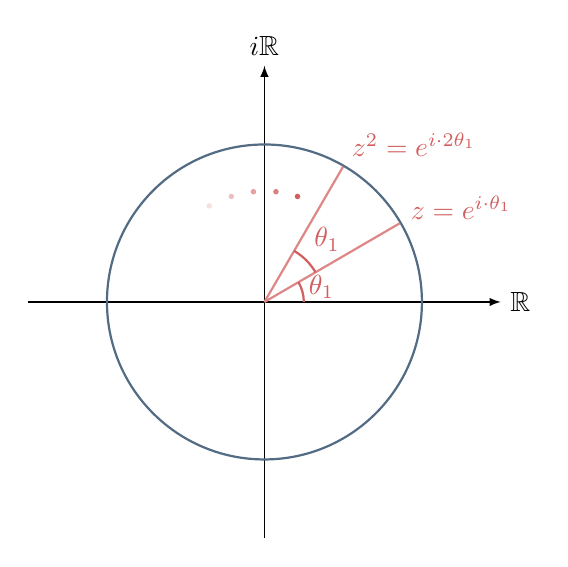
\begin{tikzpicture}[yscale=2, xscale=2]
      \coordinate (O) at (0,0);
      \coordinate (X) at (1.5,0);
      \coordinate (Z1) at (0.86, 0.5);
      \coordinate (Z2) at (0.5, 0.86);
   
      \draw[-latex] (-1.5,0) -- (X) node [right] {$\mathbb{R}$};
      \draw[-latex] (0, -1.5) -- (0,1.5) node [above] {$i\mathbb{R}$};
   
      \draw[color = DarkBlue1, thick] (0,0) circle (1cm);
   
      \draw node[color = BrightRed1] at (1.25, 0.6) {$z = e^{i\cdot\theta_1}$}; 
      \draw node[color = BrightRed1] at (0.95, 1) {$z^2 = e^{i\cdot 2\theta_1}$}; 
   
      \draw[color = BrightRed1!75, thick] (O) -- (Z1);
      \pic [color = BrightRed1, draw, thick, "$\theta_1$", angle eccentricity=1.5, angle radius=0.5cm] {angle = X--O--Z1};
   
      \draw[color = BrightRed1!75, thick] (O) -- (Z2);
      \pic [color = BrightRed1, draw, thick, "$\theta_1$", angle eccentricity=1.5, angle radius=0.75cm] {angle = Z1--O--Z2};
   
      \fill[color = BrightRed1!100] (0.21, 0.67) circle[radius=0.5pt];
      \fill[color = BrightRed1!80] (0.073, 0.70) circle[radius=0.5pt];
      \fill[color = BrightRed1!60] (-0.07, 0.70) circle[radius=0.5pt];
      \fill[color = BrightRed1!40] (-0.21, 0.67) circle[radius=0.5pt];
      \fill[color = BrightRed1!20] (-0.35, 0.61) circle[radius=0.5pt];
   \end{tikzpicture}  
\end{center}

\subsection*{\subsecstyle{Racines n-ièmes {:}}}
Soit \(n \in \N\), une partie importante des problèmes impliquant des nombres complexes proviennent d'équations d'inconnue \(Z\) de la forme:
\[
   Z^n = z
\]
On peut montrer que l'ensemble des solutions de ce type de problème est:
\customBox{width=8cm}{
   \begin{align*}
      S = \Bigl\{ \sqrt[n]{\rho}e^{i\frac{\theta + 2k\pi}{n}}\; ; \; k \in \bigl\{0, 1, \ldots , n-1 \bigl\} \Bigl\}   
  \end{align*}  
}
\underline{Cas particulier {:}}
Si on a une racine n-ième \(Z_0\) de \(Z\) et qu'on connaît les racines n-ièmes de l'unité, alors on peut obtenir toutes les racines n-ièmes de \(Z\) grâce à:

\[
   \Bigl\{ Z \in \C \; ; \; Z^n = z \Bigl\} = \Bigl\{ Z_0u \; ; \; u \in \U_n \Bigl\}   
\]

\subsection*{\subsecstyle{Le nombre complexe \(j\) {:}}}
On note \(j\) la première racine troisième de l'unité.
Le nombre \(j\) est singulier, car il vérifie:
\customBox{width=4cm}{
   \(
      j^2 = j^{-1} = \overline{j}
   \)
}

Graphiquement, on peut observer que les affixes des nombres \(1\), \(j\) et \(\overline{j}\) forment un triangle équilatéral inscrit dans le cercle trigonométrique.
\chapter*{\chapterstyle{II --- Anneau des Polynômes}} % 75% Fini
\addcontentsline{toc}{section}{Anneau des Polynômes}

\subsection*{\subsecstyle{Définition {:}}}
Soit \(K\) un corps, et \(n \in \N\), on appelle \textbf{polynômes} à coefficients dans \(K\) en l'indéterminée \(X\) les éléments de l'ensemble:
\[
   K[X] := \Biggl\{ \; \sum_{i=0}^n a_{i}X^{i} \; ; \; a_i \in K \;\Biggl\}
\]

\subsection*{\subsecstyle{Degré et Valuation {:}}}
Soit \(P, Q, R \in K[X]\).\+
On définit tout d'abord une propriété fondamentale appelée \textbf{degré} de \(P\) telle que deg\((P)\) est le plus grand coefficient non nul de P.
On a alors les propriétés du degré ci-dessous:
\customBox{width=7cm}{
   \begin{align*}
      \deg(P + Q) &\leq \max(\deg(P), \deg(Q))\\
      \deg(PQ) &= \deg(P) + \deg(Q)
  \end{align*}
}

La valuation est définie de manière analogue comme le plus petit coefficient non nul de P.
\subsection*{\subsecstyle{Opérations {:}}}
On considère ci-dessous que deg\((P)\) = \(n\) et deg\((Q)\) = \(m\) et on note \(a_i, b_i\) les coefficients de \(P\) (resp. \(Q\)).\<

On adjoint à cet ensemble une loi d'addition qui est simplement effectuée terme à termes.\+
On adjoint à cet ensemble une loi de multiplication se définit explicitement comme suit:
\[
   PQ := \sum_{k=0}^{n+m}\sum_{i+j = k} a_{i}b_{i}X^{k}
\]

Muni de ces deux opérations, on donne à cet ensemble une structure \textbf{d'anneau}\footnote[1]{Intègre car les coefficients viennent d'un corps.}.\<

On ajoute aussi une opération appelée \textbf{dérivation formelle} d'un polynôme qui s'effectue comme la dérivation analytique usuelle.
\subsection*{\subsecstyle{Divisibilité {:}}}
On définit tout d'abord une \textbf{division euclidienne} de deux polynômes qui se comporte comme la division euclidienne usuelle, à la différence que la condition d'arrêt porte sur le \textbf{degré du reste} qui doit être inférieur à celui du diviseur.\<

Soit \(U, V \in R[X]^2\), on peut aussi définir une relation de \textbf{divisibilité} entre deux polynômes, cette relation est \textbf{transitive et réflexive} et on a aussi:
\customBox{width=6.5cm}{
  \(
      D|A \land D|B \implies D| UA + VB   
  \)
}

\subsection*{\subsecstyle{Racines et Factorisation {:}}}
On dit que \(\alpha\) est une \textbf{racine} de \(P\) si \(P(\alpha) = 0\).\+
On montre alors le théorème fondamental ci-dessous:
\customBox{width=5cm}{
  \(
      P(\alpha) = 0 \Longleftrightarrow (X - \alpha) | P  
   \)
}
\pagebreak

On appelle \textbf{multiplicité d'une racine} \(\alpha\) l'entier \(m\) tel que:
\[
   \Bigr[ (X - \alpha)^m | P \Bigr] \; \land \; \Bigr[(X - \alpha)^{m+1} \nmid P\Bigr]
\]
Si on note \(P^{m}\) la dérivée n-ième de \(P\), on a aussi:
\[
   P^{m}(\alpha) = 0 \; \land \; P^{m + 1}(\alpha) \neq 0
\]

On en déduit que pour une racine \(\alpha\) de multiplicité \(m\), on peut \textbf{factoriser} \(P\) par \((X-\alpha)^m\).\<

Si on considère maintenant plusieurs racines \textbf{distinctes} \(a_0, a_1, \ldots, a_{n-1}, a_n\) de multiplicité respectivement \(m_0, m_1, \ldots, m_{n-1}, m_n\), on peut montrer la propriété suivante:
\begin{flalign*}
   \Bigr[ \prod_{i=0}^{n}(X-\alpha_i)^{m_i} \Bigr] \; \Biggr| \; P \shorteqnote{(On peut factoriser par le produit des \((X-\alpha_i)^{m_i}\))}
\end{flalign*}
\subsection*{\subsecstyle{Décomposition {:}}}
On appelle décomposition d'un polynôme \(P\) une factorisation \textbf{irréductible} de \(P\), cette décomposition dépend du corps considéré, en effet si on considère \(\C[X]\), on peut montrer le \textbf{théorème fondamental de l'Algèbre} ci-dessous:
\customBox{width=11cm}{
   Tout polynôme de degré \(n\) admet \(n\) racines dans \(\C\).
}

Par suite, on peut montrer que tout les polynômes de \(\C[X]\) sont \textbf{scindés}\footnote[1]{C'est à dire que tout les polynômes irréductibles de \(\C[X]\) sont de degré 1.}.\+
Par contre dans \(\R[X]\), il existe évidemment des polynômes de degré 2 irréductibles.\<

Soit \(z \in \C\), il existe une propriété très utile pour décomposer un polynôme \textbf{à coefficients réel} qui est:
\[
   P(z) = 0 \implies P(\overline{z}) = 0
\]
\subsection*{\subsecstyle{Fonctions symétriques des racines {:}}}
On définit le \(k\)-ième \textbf{polynôme symétrique} à \(n\) indéterminées comme la somme des produits à \(k\) facteurs de ses indéterminées, et on le note \(\sigma_k\). \<

Par exemple pour un polynôme en trois indéterminées \(a, b, c\), on a successivement:
\begin{flalign*}
    &\sigma_1 = a + b  + c\shorteqnote{(Somme des produits à 1 facteur)}\\
    &\sigma_2 = ab + ac + bc \shorteqnote{(Somme des produits à 2 facteurs)}\\
    &\sigma_3 = abc\shorteqnote{(Somme des produits à 3 facteurs)}
\end{flalign*}
De manière générale on a:
\[
    \sigma_k(x_1, \ldots, x_n) = \sum_{1 \leq i_1 < \ldots < i_k \leq n} x_{i_1}x_{i_2} \ldots x_{i_k}
\]
Soit \(P \in K[X]\) un polynôme de degré \(n\), on note \(x_1, x_2, \ldots, x_{n-1}, x_n\) ses \(n\) racines et \(a_1, a_2, \ldots, a_{n-1}, a_n\) ses \(n\) coefficients.\+
Alors, pour tout \(k \in \inticc{0}{n}\), on a le \textbf{théorème}:
\customBox{width=8cm}{
   \[\sigma_k(x_1, x_2, \ldots, x_{n-1}, x_n) = (-1)^{k}\frac{a_{n-k}}{a_n}\]
}

Ce théorème permet d'obtenir une relation \textbf{coefficient-racines}.\<

\underline{Exemple:} \(\begin{cases}
    &\text{Pour \(k = 1\), on trouve que la somme des racines de \(P\) vaut \(-\frac{a_{n-1}}{a_n}\)}\\
    &\text{Pour \(k = 2\), on trouve que la somme des doubles produits des racines de \(P\) vaut \(\frac{a_{n-2}}{a_n}\)}\\
    &\ldots\ldots\ldots\ldots\ldots\ldots
\end{cases}\)\<

   \pagebreak   

   \addcontentsline{toc}{chapter}{Algèbre Linéaire} % 85%
   \chapter*{\chapterstyle{III --- Espaces Vectoriels}} % 99% Fini
\addcontentsline{toc}{section}{Espaces Vectoriels}

\subsection*{\subsecstyle{Définition {:}}}
Soit \(E\) un ensemble \textbf{non-vide}, \(K\) un corps commutatif, et \(u \in E\), on dit alors que \((E, +, \cdot)\) est un \textbf{espace vectoriel sur K} si les conditions ci-dessous sont réunies:
\begin{align*}
   &\bullet \;\;\; (E, +) \text{ est un \textbf{groupe abélien}} \\
   &\bullet \;\; \text{ La loi \(\cdot\) est une application de \(K \times E \longrightarrow E\)} \\
   &\bullet \;\; \text{ La loi \(\cdot\) vérifie \textbf{la distributivité mixte et l'associativité mixte}} \\
   &\bullet \;\;\; 1 \cdot u = u
\end{align*}

On appelle alors \textbf{vecteurs} les éléments de \(E\) et \textbf{scalaires} les éléments de \(K\).

\subsection*{\subsecstyle{Sous-espaces vectoriels {:}}}
Soit \(F \subseteq E\), on dit que \(F\) est un \textbf{sous-espace vectoriel} si et seulement si:
\begin{align*}
   &\bullet \;\; F \text{ est non vide.} \\
   &\bullet \;\; F \text{ est stable par somme.} \\
   &\bullet \;\; F \text{ est stable par multiplication externe.}
\end{align*}

Il est utile de noter que \textbf{l'intersection} de deux sous-espaces vectoriels est aussi un sous-espace vectoriel mais que l'union de deux sous-espaces vectoriels n'est \textbf{en général} pas un sous-espace vectoriel.\<

Un cas particulier est celui du \textbf{sous-espace vectoriel engendré} par \(F\) qu'on note:
\[
   \text{Vect(\(F\))} := \Biggl\{ \sum_{i=0}^{n} \lambda_i u_i\; ; \; \lambda_{i} \in K \; , \; u_{i} \in F \Biggl\}
\]
\begin{center}
    \textit{
        C'est \textbf{l'ensemble des combinaisons linéaires} des vecteurs de \(F\).
    }
\end{center}

Soit \((A_n)_{n \in \N}\) une famille de parties de \(E\), alors on a la propriété suivante:
\customBox{width=5.5cm}{
   \[
      \sum_{i \in \N} \text{Vect(\(A_i\))} = \text{Vect\(\Bigl(\bigcup_{i \in \N} A_i\Bigl)\)}
   \]
}

Une propriété fondamentale est que Vect(\(F\)) est un \textbf{opérateur de clôture} par combinaison linéaire, ie c'est une application \textbf{idempotente, croissante et extensive}.

\subsection*{\subsecstyle{Familles libre et génératrices {:}}}
Soit \(\Fam := (u_1, u_2, \ldots, u_{n-1}, u_n)\) une famille de vecteurs de \(E\).\<

On dit que \(\Fam\) est \textbf{génératrice} de E si on a \(E = \text{Vect(\(\Fam\))}\).\+
On dit que \(\Fam\) est \textbf{libre} si tout combinaison linéaire nulle de vecteurs de \(\Fam\) est à coefficient tous nuls.\<

Formellement, \(\Fam\) est libre si et seulement si on a:
\[
    \forall (\lambda_1, \ldots, \lambda_n) \in K^n \; ; \; \Biggr[ \sum_{i=0}^n \lambda_i u_i = 0_E \implies (\lambda_1, \ldots, \lambda_n) = (0, \ldots, 0) \Biggr]  
\]
\pagebreak

Soit \(\Fam := (u_1, \ldots, u_k, \ldots, u_n)\) une famille libre et génératrice.\<

Si un vecteur \(v\) n'appartient pas à \(\text{Vect(\(\Fam\))}\), alors la famille étendue \((u_1, \ldots, u_n, v)\) est toujours libre.\+
Si un vecteur \(u_k\) appartient à \(\text{Vect(\(\Fam\))}\), alors la famille réduite \((u_1, \ldots, u_{k-1}, u_{k+1}, \ldots, u_n)\) est toujours génératrice.

\subsection*{\subsecstyle{Bases {:}}}
On appelle \textbf{base} de \(E\) une famille \textbf{libre et génératrice}, et on a le théorème suivant:
\customBox{width=8cm}{
   Tout espace vectoriel possède une base.
}

Soit \(\mathscr{B} = (e_1, e_2, \ldots, e_{n-1}, e_{n})\) une base de \(E\).\+
On appelle \textbf{coordonnées} de \(u\) dans la base \(\mathscr{B}\) les coefficients de la décomposition de \(u\) dans la base \(\mathscr{B}\) et on note:
\[
    [u]^{\mathscr{B}} = [\lambda_1 e_1 + \lambda_2 e_2 + \ldots + \lambda_{n-1} e_{n-1} + \lambda_{n-1} e_{n-1} ]^{\mathscr{B}} = 
    \begin{pmatrix}
        \lambda_1\\
        \vdots\\
        \lambda_{n}
    \end{pmatrix}
\]

\subsection*{\subsecstyle{Sommes et espaces supplémentaires{:}}}
Soit \(n\) un entier naturel et \((F_n)_{n \in \N}\) une famille de \(n\) sous-espaces vectoriels de \(E\), considérons la somme ensembliste \(S_n\) telle que:
\[
    S_n := \sum_{n\in\N} F_n := \Biggl\{ \sum_{n\in\N} u_n \; ; \; u_n \in F_n\Biggl\}
\]
Soit \((u_1, u_2, \ldots, u_n)\) un n-uplet de vecteurs quelconques du produit cartésien des \(F_n\), alors la somme est dite \textbf{directe} si et seulement si:
\customBox{width=10cm}{
   \(
      u_1 + u_2 + \ldots + u_n = 0_E \implies (u_1, u_2, \ldots, u_n) = (0, 0, \ldots, 0)
  \)
}

Et on la note alors:
\[
    S_n = \bigoplus_{n\in\N} F_n
\]

Soit \(\B_n\) des bases des \(F_n\), soit la famille \(\Fam_n = (\B_1, \B_2, \ldots, \B_n)\), \textbf{ie les bases des \(F_n\) mises ``bout à bout``}.\+
Alors on a alors le théorème suivant:
\customBox{width=7.5cm}{
   \[
      \Fam_n \text{ est une base de } S_n \Longleftrightarrow S_n = \bigoplus_{n\in\N} F_n
  \]
}

Si \textbf{l'espace entier} est engendré par \(S_n\) et que la somme est \textbf{directe}, alors on dira que les \(F_n\) sont \textbf{supplémentaires} dans \(E\).
    
\subsection*{\subsecstyle{Hyperplans {:}}}
Soit \(F\) un sous-espace vectoriel de \(E\).\+
\(F\) est un \textbf{hyperplan} de E si et seulement si il vérifie l'une des conditions équivalentes suivantes:
\begin{align*}
    &\bullet \text{ Il existe \textbf{une droite vectorielle} \(G\) de \(E\) telle que \(F \oplus G = E\).} \\
    &\bullet \text{ \(H\) est défini par une \textbf{équation linéaire homogène} non triviale.}
\end{align*}
Les hyperplans donc les \textbf{sous-espaces propres maximaux} de \(E\).

\begin{center}
    \textit{
        Résoudre un système d'équations homogènes revient donc à chercher \textbf{l'intersection} des hyperplans que représentent ces équations et donc l'ensemble des solutions est lui aussi nécessairement \textbf{un sous-espace vectoriel}.
    }
\end{center}
\chapter*{\chapterstyle{III --- Espaces Affines}} % 90 Fini
\addcontentsline{toc}{section}{Espaces affines}
Soit \(\mathscr{E}\) un ensemble non-vide et \(V\) un \(\R\)-espace vectoriel de dimension \(n\) finie.
\subsection*{\subsecstyle{Définition {:}}}
On appelle \textbf{espace affine\footnote[1]{Ses éléments sont alors appelés des \textbf{points}.} de direction} \(V\) le couple \((\mathscr{E}, +)\) avec:
\[
   \begin{aligned}
      + : &&\mathscr{E} \times V &\longrightarrow \mathscr{E}\\
      &&(\,A, \, u\,) &\longmapsto A + u
   \end{aligned}
\]
La loi + doit vérifer les axiomes suivants 
\footnote[2]{Une action d'un groupe \((G, \star)\) sur \(E\) est une application \(+\) de \(G \times E \) dans \(E\) qui vérifie: \[
   \forall g, g' \in G  \; , \; \forall x \in E \; ; \; x + (g \star g') = (x + g) \star g'
\] \hspace{15pt} En d'autres termes, additionner d'abord les vecteurs, ou d'abord le point avec le vecteur n'importe pas.}:
\customBox{width=13cm}{
   \begin{align*}
      &\textbf{Existence d'un neutre} && \forall A \in \mathscr{E} \; ; \; A + 0_V = A\\
      &\textbf{Action de groupe} && \forall A \in \mathscr{E} \; , \; \forall u,v \in V \; ; \; A + (u + v) = (A + u) + v \\
      &\textbf{Unicité du translaté} && \forall A, B \in \mathscr{E} \; , \; \exists !u \in V \; ; \; A + u = B 
   \end{align*}
}    

Etant donné deux points \(A, B \in \mathscr{E}\), on note alors \(\overrightarrow{AB}\) l'unique vecteur \(u\) qui vérifie:
\customBox{width=2.5cm}{
   \(A + u = B\)
}
On appelle alors \(A\) le \textbf{point initial} et \(B\) le \textbf{point final}

\subsection*{\subsecstyle{Propriétés {:}}}
Si \(\mathscr{E}\) est un espace affine de direction \(V\), on a alors les propriétés suivantes:
\customBox{width=8cm}{
   \begin{align*}
      &\textbf{Relation de Chasles} && \overrightarrow{AB} + \overrightarrow{BC} = \overrightarrow{AC} \\
      &\textbf{Existence d'un neutre} && \overrightarrow{AB} + \overrightarrow{BA} = O_V
    \end{align*}
}

\subsection*{\subsecstyle{Repères {:}}}
Un repère de \(\mathscr{E}\) est un couple \(\mathscr{R} = (O, \mathscr{B})\) formé d'un point \(O \in \mathscr{E}\) et d'une base \(\mathscr{B} = (e_1, \ldots, e_n)\) de \(V\). On appelle alors le point \(O\) \textbf{origine} du repère, et les vecteurs \(e_1, \ldots, e_n\) \textbf{vecteurs de base} du repère.\<

Soit \(i\in\inticc{1}{n}\), alors pour tout point \(A \in \mathscr{E}\), on appelle \textbf{coordonées} de \(A\) dans le repère \(\mathscr{R}\), les composantes \((x_i)_i\) du vecteur qui représente la translation de \(O\) vers \(A\) dans la base \(\mathscr{B}\), et on a la caractérisation élémentaire suivante:
\[
   \overrightarrow{OA} = x_1e_1 + \ldots + x_ne_n 
\]

\subsection*{\subsecstyle{Cas particulier des espaces vectoriels {:}}}
Il est important de noter que le couple \((V, +)\) forme un espace affine de \textbf{direction lui-même}. En effet, si on considère un élément de \(V\) comme un point, alors le couple  \((V, +)\) forme un espace affine de direction \(V\) et la loi \(+\) est alors exactement la loi de composition interne de \(V\).\<

L'unique vecteur \(u\) tel que \(A + u = B\) est exactement \(B - A\) (ici \(A, B\) sont des points de \(V\) qui se trouvent être des vecteurs dans ce cas particulier).
\chapter*{\chapterstyle{III --- Applications Linéaires}} % Fini 99%
\addcontentsline{toc}{section}{Applications linéaires}

Soit deux \(\K\)-espaces vectoriels \(E\) et \(F\), et \(f : E \longrightarrow F \).

\subsection*{\subsecstyle{Définition{:}}}
\addcontentsline{toc}{subsection}{Définition}

On dit que \(f\) est une \textbf{application linéaire} ou \textbf{morphisme d'espaces vectoriels} si et seulement si pour tout couple de vecteurs \(u, v \in E\) et pour tout scalaire \(\lambda\) elle vérifie: 
\customBox{width=8cm}{
   \[
      \begin{aligned}
         &\bullet \textbf{ Additivité : } f(u + v) = f(u) + f(v)\\
         &\bullet \textbf{ Homogénéité : } f(\lambda u) = \lambda f(u)\\
     \end{aligned}
  \]
}
On note alors \(\mathcal{L}(E, F)\) l'ensemble des applications linéaires de \(E\) vers \(F\).\<

On appelle \textbf{isomorphisme} tout application linéaire bijective.\+
On appelle \textbf{endomorphisme} tout application linéaire d'un ensemble dans lui-même.\+
On appelle \textbf{automorphisme} tout application linéaire bijective d'un ensemble dans lui-même\footnote[1]{On appelle l'ensemble des automorphismes \textbf{le groupe linéaire} de \(E\) qu'on note \(GL(E)\).}.\<

On appelle \textbf{forme linéaire} tout application linéaire qui a pour ensemble d'arrivée \textbf{le corps de base}\footnote[2]{On appelle l'ensemble des formes linéaires \textbf{l'espace dual} de \(E\) qu'on note \(E^*\).}.

\subsection*{\subsecstyle{Propriétés{:}}}
\addcontentsline{toc}{subsection}{Propriétés}

On s'intéresse au propriétés de l'ensemble \(\mathcal{L}(E, F)\), tout d'abord on peut prouver aisément que c'est \textbf{un sous-espace vectoriel} de l'espace des fonctions, ie il est stable par somme et par multiplication exeterne.\+
En outre, \textbf{la composée de deux applications linéaires est linéaire}.\<

Considérons une application linéaire bijective de \(\mathcal{L}(E, F)\), alors:
\begin{center}
   \textbf{Sa réciproque est nécessairement linéaire\footnote[3]{Découle directement des définitions.}}.
\end{center}

\subsection*{\subsecstyle{Image et Noyau{:}}}
\addcontentsline{toc}{subsection}{Image et Noyau}

On appelle \textbf{image} d'une application linéaire l'image telle que définie pour les applications classiques.\+
On appelle \textbf{noyau} d'une application linéaire tout \textbf{les antécédent du vecteur nul}.\+
\[
   \text{Im}(f) := \Bigl\{ f(u) \; ; \; u \in E \Bigl\}
   \quad\quad\quad\quad\quad
   \text{Ker}(f) := \Bigl\{ u \in E \; ; \; f(u) = 0_F \Bigl\}
\]
On voit directement que \(\text{Im}(f)\) est un \textbf{sous-espace vectoriel} de l'ensemble d'arrivée et que \(\text{Ker}(f)\) est un \textbf{sous-espace vectoriel} de l'ensemble de départ.\<

En particulier si \(E = \text{Vect}(e_1, e_2, \ldots, e_n)\) pour une certaine famille \((e_i)_{i\in \N}\), alors on a\footnote[5]{Idem.}:
\customBox{width=11cm}{
   \(
      \text{Im}(f) = f(\text{Vect}(e_1, e_2, \ldots, e_n)) = \text{Vect}(f(e_1), f(e_2), \ldots, f(e_n))
  \)
}

Une propriété fondamentale du noyau\footnote[6]{De manière générale, cette propriété est vraie pour le noyau de tout morphisme de groupe, on peut alors voir la ``taille'' du noyau comme \textbf{une mesure de la non-injectivité} du morphisme.} est la suivante:
\customBox{width=15.5cm}{
   Une application linéaire est injective si et seulement si son noyau est réduit au vecteur nul.
}
\pagebreak

\subsection*{\subsecstyle{Caractérisations par les familles{:}}}
\addcontentsline{toc}{subsection}{Caractérisations par les familles}

Soit \(\mathscr{F} = (e_i)_{i \in \N}\) une famille de \(E\) et un endomorphisme de \(E\), alors \(f\) est entièrement caractérisée par l'image de cette famille, en effet on a:
\begin{itemize}
   \item L'image d'une famille libre est libre \(\Longleftrightarrow f\) est injective.
   \item L'image d'une famille génératice est génératice \(\Longleftrightarrow f\) est surjective.      
\end{itemize}

\subsection*{\subsecstyle{Endomorphismes remarquables{:}}}
\addcontentsline{toc}{subsection}{Endomorphismes remarquables}

On considère ici des endomorphismes remarquables comme:
\begin{itemize}
   \item Les homotéthies: Elles sont caractérisées par \(\varphi_k : u \longmapsto ku\)
   \item Les symétries: Elles sont caractérisées par \(\varphi \circ \varphi = \text{Id}_E\)
   \item Les projecteurs: Elles sont caractérisées par \(\varphi \circ \varphi = \varphi\)
\end{itemize}
Précisons le cas des projecteurs, en effet si on considère deux sous-espaces \(F, G\) supplémentaires dans \(E\), alors chaque élément \(u \in E\) admet une décomposition unique de la forme \(u = v_F + v_G\).\<

Alors le projecteur de direction \(F\) sur \(G\) est exactement l'application \(\varphi\) telle que:
\[
   \varphi(u) = v_G
\]
Graphiquement, pour \(\varphi\) le projecteur de direction \(F\) sur \(G\):
\begin{center}
   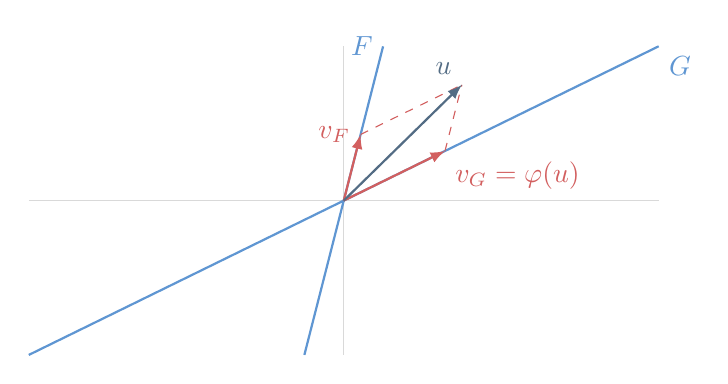
\begin{tikzpicture}[yscale=0.98]
      \draw[black!15] (-4,0) -- (4,0);
      \draw[black!15] (0, -2) -- (0,2);

      \draw[color=BrightBlue1, domain=-0.5:0.5, thick] plot (\x,{4*\x}) node[left] {$F$};
      \draw[color=BrightBlue1, domain=-4:4, thick] plot (\x,{0.5*\x}) node[below right] {$G$};

      \draw[-latex, color=BrightRed1, thick] (0, 0) -- (3/14, 6/7) node[left] {$v_F$};
      \draw[-latex, color=BrightRed1, thick] (0, 0) -- (9/7, 9/14) node[below right] {$v_G = \varphi(u)$};

      \draw[color=BrightRed1, dashed] (9/7, 9/14) -- (1.5, 1.5);
      \draw[color=BrightRed1, dashed] (3/14, 6/7) -- (1.5, 1.5);

      \draw[-latex, color=DarkBlue1, thick] (0, 0) -- (1.5,1.5) node[above left] {$u$};
   \end{tikzpicture} 
\end{center}

\subsection*{\subsecstyle{Applications multilinéaires{:}}}
\addcontentsline{toc}{subsection}{Applications multilinéaires}

On peut généraliser le concept de linéarité à celui de \textbf{multilinéarité} ou \textbf{n-linéarité}. On considère alors une application de la forme \(f : E^n \longrightarrow F\), alors on dit que \(f\) est multilinéaire si et seulement si elle est linéaire \textbf{en chacune des variables}, ie si:
\begin{align*}
   f(e_1 + \lambda u, e_2, \ldots, e_n) &= f(e_1, e_2, \ldots, e_n) + \lambda f(u, e_2, \ldots, e_n)  \\
   f(e_1, e_2  + \lambda u, \ldots, e_n) &= f(e_1, e_2, \ldots, e_n) + \lambda f(e_1, u, \ldots, e_n) \\
   & \vdotswithin{=} \\   
   f(e_1, e_2 , \ldots, e_n + \lambda u) &= f(e_1, e_2, \ldots, e_n) + \lambda f(e_1, e_2, \ldots, u)
\end{align*}
Une telle application est dite:
\begin{itemize}
   \item \textbf{Symétrique} si permuter deux variables préserve le résultat.\footnote[1]{\underline{Exemple:} \(f(e_1, e_2) = f(e_2, e_1)\)}
   \item \textbf{Antisymétrique} si permuter deux variables change le signe du résultat.\footnote[2]{\underline{Exemple:} \(f(e_1, e_2) = -f(e_2, e_1)\), en particulier, le signe du résultat aprés une permutation \(\sigma\) dépends alors de \textbf{la signature de la permutation} (la parité du nombre de permutations effectuées).}
   \item  \textbf{Altérnée} si elle s'annule à chaque fois qu'on l'évalue sur un k-uplet contenant deux vecteurs identiques.\footnote[3]{\underline{Exemple:} \(f(e_1, e_1) = 0\)}
\end{itemize}
\chapter*{\chapterstyle{III --- Théorie de la dimension}} % Fini 99%
\addcontentsline{toc}{section}{Théorie de la dimension}

Dans ce chapitre, on considérera un espace vectoriel \(E\) qui admet une famille génératrice \textbf{finie}. On dira alors que \(E\) est de \textbf{dimension finie}.

\subsection*{\subsecstyle{Théorème de la base incomplète{:}}}
\addcontentsline{toc}{subsection}{Théorème de la base incomplète}

Soit \(\mathcal{L}\) une famille libre et \(\mathcal{G}\) une famille génératrice de \(E\), le concept de \textbf{dimension} se définit gràce au \textbf{théorème de la base incomplète}:
\begin{itemize}
   \item On peut \textbf{compléter} \(\mathcal{L}\) en une base de \(E\) par ajouts de vecteurs de \(\mathcal{G}\).
   \item On peut \textbf{extraire} de \(\mathcal{G}\) une base de \(E\) (corollaire immédiat).
\end{itemize}
Ce théorème permet alors d'assurer \textbf{l'existence} d'une base d'une espace vectoriel de dimension finie.

\subsection*{\subsecstyle{Théorème de la dimension{:}}}
\addcontentsline{toc}{subsection}{Théorème de la dimension}

Il est évident que le cardinal d'une partie libre est toujours inférieur au cardinal d'une partie génératrice \footnote[1]{Aussi appellé \textbf{lemme de Steiniz}.}, de cette considération, on peut alors montrer \textbf{le théorème de la dimension}:
\customBox{width=13cm}{
   Toutes les bases d'un espace vectoriel de dimensions fini ont \textbf{même cardinal}.
}
Ce théorème permet alors d'assurer \textbf{l'unicité} du cardinal des bases d'une espace vectoriel de dimension finie.

\subsection*{\subsecstyle{Définition de la dimension{:}}}
\addcontentsline{toc}{subsection}{Définition de la dimension}

Des deux théorèmes précédents, on a alors l'existence de bases d'une espace de dimension fini, et l'unicité de leur cardinal, on peut alors définir \textbf{la dimension d'une espace vectoriel} comme ce cardinal et on la note \(\text{dim}(E)\).\<

On peut alors en déduire la dimension des espaces vectoriels communs:
\begin{itemize}
   \item L'espace vectoriel classique \(\K^n\) est de dimension \(n\).
   \item L'espace vectoriel des polynômes de degré au plus \(n\) est de dimension \(n + 1\).
   \item Une droite vectorielle est de dimension \(1\).
   \item Un plan vectoriel est de dimension \(2\).
\end{itemize}

\subsection*{\subsecstyle{Espaces de dimension finie{:}}}
\addcontentsline{toc}{subsection}{Espaces de dimension finie}

Considérons maintenant \(E\) un espace vectoriel de dimension finie \(n\) est \(\Fam = (e_i)_{i \in \N}\) une famille de \(n\) vecteurs de \(E\).\+
Alors par déduction immédiate\footnote[2]{En effet par exemple sachant qu'elle est libre et possède \(n\) vecteurs, si ce n'était pas une base, on pourrait rajouter un/des vecteur pour obtenir une base, et donc dim\((E) \neq n \implies \bot\).} de la définition de dimension, on a:
\customBox{width=11cm}{
   \(\Fam\) est libre \(\Longleftrightarrow\) \(\Fam\) est génératrice \(\Longleftrightarrow\) \(\Fam\) est une base.
}
En effet, intuitivement on comprends que si une famille possède \textbf{le bon nombre de vecteurs}, alors il suffit qu'elle soit libre (ou génératrice) pour que ce soit une base.\<

Soient \(F, G\) deux sous-espaces de \(E\). La dimension permet aussi de prouver des \textbf{égalités} d'espaces vectoriels, gràce à la propriété:
\[
   \begin{rcases}
      F \subset G \\
      \text{dim}(F) = \text{dim}(G)
   \end{rcases}\implies F = G
\]
Aussi, on peut alors \textbf{caractériser} le fait que \(F\) et \(G\) soient \textbf{supplémentaires} dans \(E\) par:
\[
   F \oplus G = E \Longleftrightarrow \begin{cases}
      F \cap G = \{0_E\}\\
      \text{dim}(F) + \text{dim}(G) = \text{dim}(E)
   \end{cases}
\]
Enfin on peut calculer \textbf{la dimension d'une somme}\footnote[1]{Le cas d'égalité est intéressant car il intervient pour des sous-espaces d'intersection nulle, et alors la dimension de la somme est simplement égale à la somme des dimensions.} avec la \textbf{formule de Grassmann}:
\customBox{width=8cm}{
   \(
      \text{dim}(F + G) = \text{dim}(F) + \text{dim}(G) - \text{dim}(F \cap G)
   \)
}


\subsection*{\subsecstyle{Rang {:}}}
\addcontentsline{toc}{subsection}{Rang}

Soit \(E\) un espace vectoriel de dimension finie et \(\Fam = (e_i)_{i \in \N}\) une famille de vecteurs de cet espace, alors on appelle \textbf{rang} de \(\Fam\) l'entier:
\customBox{width=5cm}{
   \(\text{rg}(\Fam) = \text{dim}(\text{Vect}(\Fam))\)
}

Informellement, le rang est simplement \textbf{la dimension de l'espace engendré par la famille}.\<

On étends cette définition à celle du \textbf{rang d'une application linéaire}, qu'on note \(\text{rg}(f)\), qui correspond à \textbf{la dimension de son image}, et on définit ainsi une application linéaire \textbf{de rang fini}.

\subsection*{\subsecstyle{Applications linéaires en dimension finie{:}}}
\addcontentsline{toc}{subsection}{Applications linéaires en dimension finie}

Soit \(f \in \mathcal{L}(E, F)\) une telle application, alors on peut montrer le \textbf{théorème du rang}:
\customBox{width=7cm}{
   \(
      \text{dim}(E) = \text{rg}(f) + \text{dim}(\text{Ker}(f))
   \)
}

Ce thèorème permet alors de caractériser l'injectivité et la surjectivité d'une application linéaire par:
\begin{itemize}
   \item \(f\) est injective si et seulement si \(\text{rg}(f) = \text{dim}(E)\)
   \item \(f\) est surjective si et seulement si \(\text{rg}(f) = \text{dim}(F)\)
\end{itemize}

En particulier, si \(E\) et \(F\) sont deux espaces vectoriels \textbf{de même dimension} alors:
\customBox{width=10cm}{
   \(f\) est injective \(\Longleftrightarrow\) \(f\) est surjective \(\Longleftrightarrow\) \(f\) est bijective
}
On caractérise ainsi \textbf{les isomorphismes en dimension finie}\footnote[2]{Toutes ces propriétés n'étant que de simples applications du théorème du rang.}.
\chapter*{\chapterstyle{III --- Espace des matrices}} % Fini 99%
\addcontentsline{toc}{section}{Espace des matrices}

On appelle \textbf{matrice} à \(n\) lignes et \(p\) colonnes à coefficients dans \(\K\) toute application \(M : \inticc{1}{n} \times \inticc{1}{p} \longrightarrow \K\), en d'autres termes \textbf{tout famille de scalaires indexée par }\(\inticc{1}{n} \times \inticc{1}{p}\).\<

Informellement, il s'agit d'une généralisation du concept de suite sous forme de suite à \textbf{deux indices}, qu'on peut alors voir comme un tableau de nombres tel qu'en chaque position \((i, j)\), on ait un scalaire \(a_{ij} \in \K\).\< 

A l'instar des suites, on note \(M = (a_{ij})_{\substack{1 \leq i \leq n\\1 \leq j \leq p}}\) pour faire référence au terme général de \(M\) en position \((i,j)\).

\subsection*{\subsecstyle{Définition et propriétés{:}}}
\addcontentsline{toc}{subsection}{Définition}

On appelle \textbf{espace des matrices} à \(n\) lignes et \(p\) colonnes à coefficient dans \(\K\), et on note \(\mathcal{M}_{n, p}(\K)\), l'espace de toutes les matrices comme définies ci-dessus.\<

On définit \textbf{la somme} de deux matrices comme la matrice dont le terme en position \((i, j)\) est la sommes des termes des deux matrices en cette position, informellement, on additionne simplement \textbf{composante par composante}.\+
On définit \textbf{la multiplication} d'une matrice par un scalaire comme la matrice dont tout les termes sont multipliés par ce scalaire.\<

Pour ces deux lois l'ensemble \((\mathcal{M}_{n, p}(\K), +, \cdot)\) est alors muni d'une structure \textbf{d'espace vectoriel} sur \(\K\) (de dimension \(n \times p\)) ayant pour vecteur nul \(0_E\) la matrice dont tout les coefficients sont nuls.

\subsection*{\subsecstyle{Produit matriciel{:}}}
\addcontentsline{toc}{subsection}{Produit matriciel}

Soit \(A = (a_{i, j}) \in \mathcal{M}_{n, m}(\K)\) et \(B = (b_{k, j}) \in \mathcal{M}_{m, p}(\K)\).\+
Alors on définit\footnote[1]{Il faut que le nombre de colonnes de la première soit égal au nombre de lignes de la seconde pour que les matrices soient dites \textbf{compatibles}.}  la matrice \(C := AB = (c_{i,j})\) comme étant la matrice telle que:
\customBox{width=3.5cm}{
   \[
      c_{i, j} = \sum_{k=1}^{n}a_{i, k}b_{k, j}
   \]
}

En particulier, on appelle ce produit \textbf{un produit ligne par colonne} qui se comprends visuellement par:\+
\begin{center}
   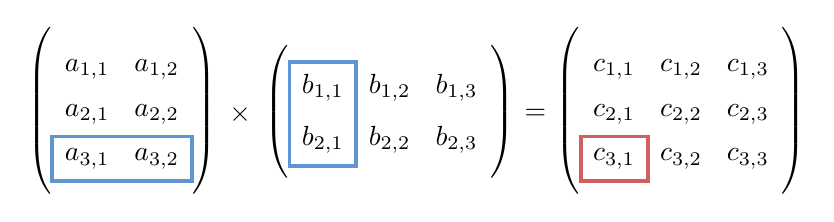
\begin{tikzpicture}[    
      every left delimiter/.style={xshift=.55em},
      every right delimiter/.style={xshift=-.55em}
    ]
      \matrix[
        matrix of math nodes, ampersand replacement=\&,
        left delimiter=(, right delimiter=),  outer sep = 0pt,inner sep=4.5pt
      ](A){
        a_{1, 1} \& a_{1, 2}\\ 
        a_{2, 1} \& a_{2, 2}\\ 
        a_{3, 1} \& a_{3, 2}\\  
      };
      \draw[color=BrightBlue1, line width=0.5mm] (A-3-1.south west) rectangle (A-3-2.north east);
      \draw node at (1.5, 0) {\(\times\)};
  
      \matrix[
        matrix of math nodes, ampersand replacement=\&,
        left delimiter=(, right delimiter=),  outer sep = 0pt,inner sep=4.5pt
      ] (B) at (3.4, 0) {
        b_{1, 1} \& b_{1, 2} \& b_{1, 3}\\ 
        b_{2, 1} \& b_{2, 2} \& b_{2, 3}\\ 
      };
      \draw[color=BrightBlue1, line width=0.5mm] (B-1-1.north west) rectangle (B-2-1.south east);
  
      \draw node at (5.25, 0) {\(=\)};
  
      \matrix[
        matrix of math nodes, ampersand replacement=\&,
        left delimiter=(, right delimiter=),  outer sep = 0pt,inner sep=4.5pt
      ] (C) at (7.1, 0) {
        c_{1, 1} \& c_{1, 2} \& c_{1, 3}\\ 
        c_{2, 1} \& c_{2, 2} \& c_{2, 3}\\ 
        c_{3, 1} \& c_{3, 2} \& c_{3, 3}\\
      };
      \draw[color=BrightRed1, line width=0.5mm] (C-3-1.north west) rectangle (C-3-1.south east);
    \end{tikzpicture}
\end{center}
Le coefficient à \color{BrightRed1} la troisième ligne, première colonne \color{black} est obtenu en multipliant \color{BrightBlue1} la troisième ligne par la première colonne.\color{black}\<

On appelle \textbf{matrice identité} la matrice neutre pour cette opération, c'est la matrice composée uniquement de \(1\) sur toute la diagonale principale, et de \(0\) partout ailleurs.\<

En considérant cette définition, il est évident que le produit matrice n'est en général \textbf{pas commutatif}. Par ailleurs \textbf{le produit de deux matrices non nulles peut être nul}.
\pagebreak

Sous réserve de compatibilités des tailles matrices, on a les propriétés suivantes:
\begin{multicols}{2}
   \begin{itemize}
      \item Associativité
      \item La matrice identité est neutre
      \item Distributivité
      \item La matrice nulle est absorbante
   \end{itemize}
\end{multicols}   

Considérons maintenant des matrices \textbf{carrées} de même taille, le produit est alors toujours défini et on peut définir une \textbf{puissance positive de matrice}, qu'on note \(A^n\) qui vérifie alors:

\begin{multicols}{2}
   \begin{itemize}
      \item \((A^p)^q = A^{pq}\)
      \item \(A^pA^q = A^{p +q}\)
   \end{itemize}
\end{multicols}    

\subsection*{\subsecstyle{Transposition{:}}}
\addcontentsline{toc}{subsection}{Transposition}

Soit \(M = (x_{i,j})\in \mathcal{M}_{n, m}(\K)\), on définit maintenant \textbf{l'opération de transposition} d'une matrice notée \(M^\mathsf{T}\), c'est \textbf{une application linéaire involutive} définie par:
\customBox{width=3cm}{
   \(
      M^\mathsf{T} = (x_{j,i})
   \)
}

Intuitivement, cette application transforme \textbf{chaque ligne en colonne et invérsement}. Par exemple:
\[
   \begin{pmatrix}
      a & b & c\\
      d & e & f
   \end{pmatrix}^\top = 
   \begin{pmatrix}
      a & d\\
      b & e\\
      c & f
   \end{pmatrix}
\]
Il faut aussi noter son comportement par rapport au produit matriciel de deux matrices \(A, B\), précisément on a:
\customBox{width=3.5cm}{
   \(
      (AB)^\top = B^\top A^\top
   \)
}


\subsection*{\subsecstyle{Trace{:}}}
\addcontentsline{toc}{subsection}{Trace}

On définit aussi une autre application linéaire appellée \textbf{trace d'une matrice}, et qui est définie comme \textbf{la somme des éléments diagonaux}. Formellement:
\[
   \text{tr}(A) := \sum_{i=1}^{n} a_{i, i}   
\]
Elle est donc linéaire mais on a aussi:
\customBox{width=3.5cm}{
   \(
      \text{tr}(AB) = \text{tr}(BA)  
   \)
}


\subsection*{\subsecstyle{Matrice d'une famille de vecteurs{:}}}
\addcontentsline{toc}{subsection}{Matrice d'une famille de vecteurs}

Soit \(\mathscr{F} = (e_i)_{i\in\N}\), alors on peut définir \textbf{la matrice de la famille} dans une base \(\mathscr{B}\) par:
\customBox{width=7cm}{
   \(
      \text{Mat}_{\mathscr{B}}(\mathscr{F}) = ([e_1]_{\mathscr{B}}, [e_2]_{\mathscr{B}}, \ldots, [e_n]_{\mathscr{B}})  
   \)
}

\begin{center}
   \textit{
      La matrice d'une famille est donc constituée des coordonées des vecteurs\+
      dans la base donnée (en colonnes).
   }
\end{center}
\pagebreak

\subsection*{\subsecstyle{Matrice d'une application linéaire{:}}}
\addcontentsline{toc}{subsection}{Matrice d'une application linéaire}

Soit \(E, F\) deux espaces vectoriels (de bases \(\mathscr{B} = (e_i)_{i \in \N}\) et \(\mathscr{C}=(f_i)_{i \in \N}\)) et \(f \in \mathcal{L}(E, F)\).\<

Alors on peut associer à l'application \(f\) \textbf{une unique matrice} dans les bases \(\mathscr{B, C}\), qu'on note alors Mat\(_{\mathscr{B, C}}(f)\) qu'on construit comme suit:
\customBox{width=9cm}{
   \(
      \text{Mat}_{\mathscr{B, C}}(f) = ([f(e_1)]_{\mathscr{C}}, [f(e_2)]_{\mathscr{C}}, \ldots, [f(e_n)]_{\mathscr{C}})
   \)
}
\begin{center}
   \textit{
      La matrice d'une application linéaire est donc constituée des coordonées dans la base d'arrivée de l'image des vecteurs de la base de départ (en colonnes).
   }
\end{center}

\underline{Exemple:} Considérons un endomorphisme de \(\R^3\) et sa base canonique notée \((e_1, e_2, e_3)\), telle que \(f(x, y, z) = (2x+1, 3x, z-1)\). Alors on calcule l'image des vecteurs de la base de départ, ie:
\begin{multicols}{3}
\begin{itemize}
   \item \(f(1, 0, 0) = (3, 3, -1)\)
   \item \(f(0, 1, 0) = (0, 0, -1)\)
   \item \(f(0, 0, 1) = (0, 0, -2)\)
\end{itemize}
\end{multicols}
Puis on calcule les coordonées de ces vecteurs dans la base d'arrivée, et on les range en colonne dans une matrice et on obtient:
\begin{center}
   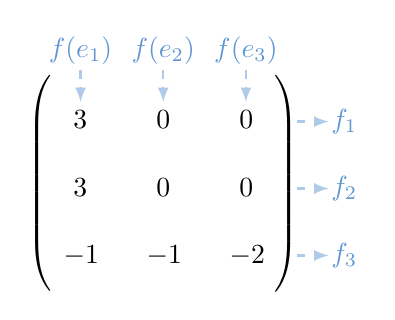
\begin{tikzpicture}[      
      every left delimiter/.style={xshift=.55em},
      every right delimiter/.style={xshift=-.55em}
    ]
    \draw node[color = BrightBlue1] at (-1.05, 1.75) {$f(e_1)$};
    \draw[-latex, dashed, thick, color = BrightBlue1!50] (-1.05, 1.5) -- (-1.05, 1.1);
  
    \draw node[color = BrightBlue1] at (0, 1.75) {$f(e_2)$};
    \draw[-latex, dashed, thick, color = BrightBlue1!50] (0, 1.5) -- (0, 1.1);
  
    \draw node[color = BrightBlue1] at (1.05, 1.75) {$f(e_3)$};
    \draw[-latex, dashed, thick, color = BrightBlue1!50] (1.05, 1.5) -- (1.05, 1.1);
  
    \draw node[color = BrightBlue1] at (2.3, 0.85) {$f_1$};
    \draw[-latex, dashed, thick, color = BrightBlue1!50] (1.7, 0.85) -- (2.1, 0.85);
  
    \draw node[color = BrightBlue1] at (2.3, 0) {$f_2$};
    \draw[-latex, dashed, thick, color = BrightBlue1!50] (1.7, 0) -- (2.1, 0);
  
    \draw node[color = BrightBlue1] at (2.3, -0.85) {$f_3$};
    \draw[-latex, dashed, thick, color = BrightBlue1!50] (1.7, -0.85) -- (2.1, -0.85);
  
    \matrix[
      matrix of math nodes, ampersand replacement=\&,
      left delimiter=(, right delimiter=), inner ysep=4pt, column sep=0.8em, row sep = 0.8em,
      nodes={
        inner sep=0.5em,outer sep=0,text width=1.2em,align=center
      }
    ]{
      3 \& 0 \& 0\\ 
      3 \& 0 \& 0\\ 
      -1 \& -1 \& -2\\
    };
    \end{tikzpicture}
\end{center}


Cette construction implique qu'il suffit donc, pour une base donnée, de \textbf{calculer les images des vecteurs de cette base}, puis leur coordonées pour décrire la transformation.\<

Si \(E\) et \(F\) sont de dimensions respectives \(n\) et \(p\), on peut alors construire \textbf{un isomorphisme fondamental}:
\customBox{width=7cm}{
   \(
      \text{Mat}_{\mathscr{B, C}} : \mathcal{L}(E, F) \xlongrightarrow{\sim} \mathcal{M}_{n, p}(\K) 
   \)
}

\begin{center}
   \textit{On peut alors considèrer, que du point de vue de l'algèbre linéaire, l'espace des application linéaires et l'espace des matrices sont identiques\footnote[1]{En dimension finie}.}
\end{center}

Dans la suite, pour plus de lisibilité, on considèrera un endomorphisme \(f\) de \(\R^2\) de matrice \(M\) dans la base canonique \(\mathscr{C}\).
Alors, appliquer une transformation linéaire à un vecteur \(u \in E\) revient à \textbf{multiplier ce vecteur par la matrice associée}\footnote[2]{Il suffit de partir du produit matriciel et d'utiliser la définition de \(M\) comme étant la matrice de \(f\) et les règles de calculs sur les vecteurs colonnes.}, ie on a:
\customBox{width=4cm}{
   \(
      [f(u)]_{\mathscr{C}} = M \times [u]_{\mathscr{C}}
   \)
}

\underline{Exemple:} Soit \(f\) de matrice 
\(M = \begin{pmatrix}
   1 & 2\\
   3 & 4\\
\end{pmatrix}\) 
et \(u = (5, 3)\), calculer les coordonées de \(f(u)\) revient à calculer:
\[
   \begin{pmatrix}
      1 & 2\\
      3 & 4\\
   \end{pmatrix}
   \begin{pmatrix}
      5 \\
      3 \\
   \end{pmatrix} =
   \begin{pmatrix}
      11 \\
      27 \\
   \end{pmatrix} 
\]
Enfin l'isomorphisme entre ces deux espaces nous permet de définir \textbf{le noyau et l'image d'une matrice}, comme simplement étant le noyau ou l'image de l'application linéaire associée à cette matrice.

\subsection*{\subsecstyle{Matrices inversibles{:}}}
\addcontentsline{toc}{subsection}{Matrices inversibles}

Soit \(M \in \mathcal{M}_n(\K)\) une matrice carrée, alors on dit que \(M\) est \textbf{inversible} si il existe un inverse pour la loi de multiplication des matrices, ie si il existe une matrice \(A^{-1}\) telle que:
\customBox{width=3.5cm}{
   \(
      AA^{-1}=\text{Id}_n
   \)
}

En particulier, si on considère l'application linéaire associée à \(M\), alors:
\begin{center}
   \(M\) inversible \(\Longleftrightarrow\) \(f\) est inversible
\end{center}

On appelle l'ensemble des matrices carrées inversibles de taille \(n\) \textbf{le groupe linéaire} d'ordre \(n\), qu'on note GL\(_n(\K)\), c'est un groupe pour la multiplication matricielle, ie on a:
\[
   A, B \in \text{GL}_n(\K) \Longleftrightarrow AB \in \text{GL}_n(\K)
\]
Et en particulier, on montre\footnote[1]{Intuitivement, c'est équivalent à l'inverse d'une composée car les matrices ``sont'' des applications au sens de l'algèbre linéaire.} que \((AB)^{-1} = B^{-1}A^{-1}\). Dans le cas d'une matrice inversible, on peut alors étendre notre définition de puissance d'une matrice au cas d'entiers négatifs.\<

Intuitivement:
\begin{center}
   \textit{Le groupe \(\text{GL}_n(\K)\) est donc le groupe \textbf{des automorphismes} de \(E\), c'est à dire le groupe \textbf{des transformations} (linéaires) de \(E\) qui sont \textbf{réversibles}.}
\end{center}
Visuellement, on comprends directement l'idée d'automorphisme d'un espace, son lien avec la bijectivité, la matrice inverse est alors la représentation algèbrique de la transformation inverse (ici avec une rotation de \(\R^2\) de \(45\) degrés):
\begin{center}
   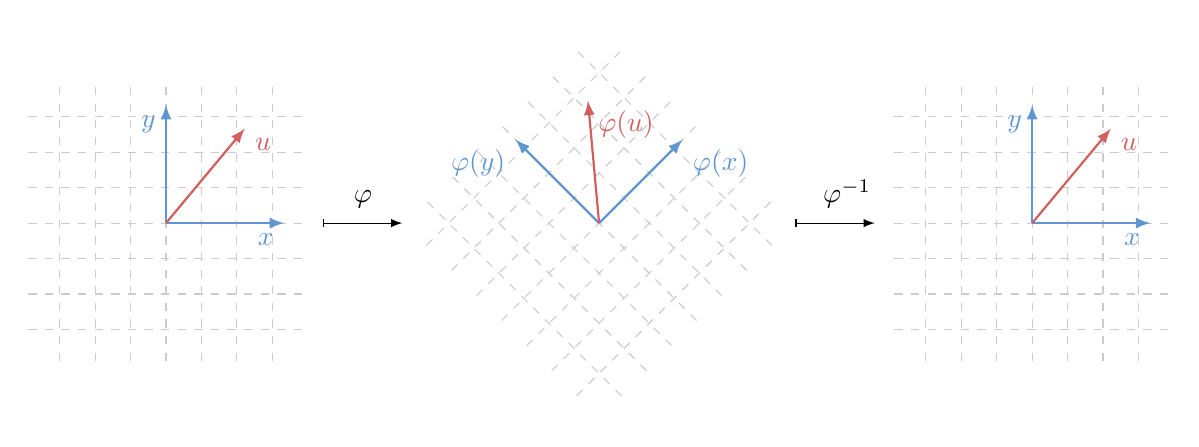
\begin{tikzpicture}
      \draw[step=0.45cm, color=black!20, dashed] (-1.75,-1.75) grid (1.75,1.75);
      \draw[-latex, color=BrightBlue1, thick] (0,0) -- (0,1.5) node[below left] {$y$};
      \draw[-latex, color=BrightBlue1, thick] (0,0) -- (1.5,0) node[below left] {$x$};
      \draw[-latex, color=BrightRed1, thick] (0,0) -- (1,1.2) node[below right] {$u$};
  
      \draw[-latex] (2,0) -- (3,0);
      \draw[] (2,-0.05) -- (2,0.05);
      \draw[] node[] at (2.5,0.3){$\varphi$};
  
      \draw[step=0.45cm, color=black!20, dashed, shift={(5.5 cm, 0)}, rotate=45] (-1.75,-1.75) grid (1.75,1.75);
      \draw[-latex, color=BrightBlue1, thick, shift={(5.5 cm, 0)}, rotate=45] (0,0) -- (0,1.5) node[below left] {$\varphi(y)$};
      \draw[-latex, color=BrightBlue1, thick, shift={(5.5 cm, 0)}, rotate=45] (0,0) -- (1.5,0) node[below right] {$\varphi(x)$};
      \draw[-latex, color=BrightRed1, thick, shift={(5.5 cm, 0)}, rotate=45] (0,0) -- (1,1.2) node[below right] {$\varphi(u)$};
  
      \draw[-latex] (8,0) -- (9,0);
      \draw[] (8,-0.05) -- (8,0.05);
      \draw[] node[] at (8.65,0.375){$\varphi^{-1}$};
  
      \draw[step=0.45cm, color=black!20, dashed, shift={(11 cm, 0)}] (-1.75,-1.75) grid (1.75,1.75);
      \draw[-latex, color=BrightBlue1, thick, shift={(11 cm, 0)}] (0,0) -- (0,1.5) node[below left] {$y$};
      \draw[-latex, color=BrightBlue1, thick, shift={(11 cm, 0)}] (0,0) -- (1.5,0) node[below left] {$x$};
      \draw[-latex, color=BrightRed1, thick, shift={(11 cm, 0)}] (0,0) -- (1,1.2) node[below right] {$u$};
    \end{tikzpicture}   
\end{center}
Enfin, on peut montrer que \textbf{la transposition} est compatible avec l'inverse, ie on a:
\customBox{width=4cm}{
   \(
      (M^{-1})^{\top} = (M^{\top})^{-1} 
   \)
}  
Montrer qu'une matrice est inversible consiste simplement à calculer \textbf{le rang de la matrice}, comme expliqué dans la partie suivante.\+ 
Par ailleurs, calculer l'inverse peut se réaliser de plusieurs manières, la méthode la plus générale consiste à résoudre l'équation d'inconnue \(X\) de la forme:
\[
   AX = Y   
\]

On définira aussi une application fondamentale nommée \textbf{déterminant} qui sera définie dans le prochain chapitre et qui caractérise exactement toutes les matrices inversibles et donne une autre manière de calculer l'inverse.
\pagebreak

\subsection*{\subsecstyle{Rang d'une matrice{:}}}
\addcontentsline{toc}{subsection}{Rang d'une matrice}

On a défini précédemment le concept de rang d'un famille et de rang d'une application linéaire, on peut généraliser cette définition en celle de \textbf{rang d'une matrice}, en effet on a simplement:
\begin{center}
   \textit{Le rang d'une matrice est la dimension de l'espace de ses colonnes.}
\end{center}

Soit \(M \in \mathcal{M}_n(\K)\), dont on note les colonnes \(\Fam = (C_1, C_2, \ldots, C_n)\), alors si le rang de la matrice est \(n\), on peut en déduire plusieurs propriétés:
\begin{multicols}{2}
   \begin{itemize}
      \item La matrice est inversible.
      \item La famille \(\Fam\) est une base de \(\K^n\).
   \end{itemize}
\end{multicols}
On remarque donc que le rang nous donne \textbf{énormément d'informations} sur la matrice, la famille des colonnes, et l'application linéaire associée.

\subsection*{\subsecstyle{Matrice de passage{:}}}
\addcontentsline{toc}{subsection}{Matrice de passage}

On considère un espace vectoriel \(E\) et deux bases \(\Fam=(e_1, \ldots, e_n), \Fam'=({e}_1', \ldots, {e}_n')\) de cet espace.\+
On appelle \textbf{matrice de passage} de \(\Fam\) à \(\Fam'\) la matrice \(P\) qu'on construit comme suit:
\customBox{width=7cm}{
   \(
      \text{Pass}(\Fam, \Fam') = ([e_1']_{\Fam}, [e_2']_{\Fam}, \ldots, [e_n']_{\Fam}) 
   \)
} 
\begin{center}
   \textit{
      La matrice de passage est donc constituée des coordonées dans l'ancienne base des vecteurs de la nouvelle base(en colonnes).
   }
\end{center}

\underline{Exemple:} Considèrons deux bases de \(\R^2\) telles que \(\Fam = [(1, 2), (3, 4)]\) et \(\Fam' = [(5, 6), (7, 8)]\), alors on a:
\[
   [5, 6]_\Fam = \begin{pmatrix} -1 \\ 2\end{pmatrix}
   \quad\quad\quad\quad
   [7, 8]_\Fam = \begin{pmatrix} 3 \\ -2\end{pmatrix}
\]
On range ensuite ces coordonées en colonnes dans la matrice, et on obtient:
\begin{center}
   \vspace{-5pt}   
   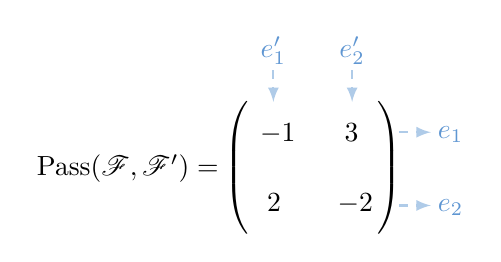
\begin{tikzpicture}[      
      every left delimiter/.style={xshift=.55em},
      every right delimiter/.style={xshift=-.55em},
   ]
   \draw node[] at (-2.35, 0) {$\text{Pass}(\Fam, \Fam') = $};

   \draw node[color = BrightBlue1] at (-0.5, 1.5) {$e_1'$};
   \draw[-latex, dashed, thick, color = BrightBlue1!50] (-0.5, 1.25) -- (-0.5, 0.85);

   \draw node[color = BrightBlue1] at (0.5, 1.5) {$e_2'$};
   \draw[-latex, dashed, thick, color = BrightBlue1!50] (0.5, 1.25) -- (0.5, 0.85);

   \draw node[color = BrightBlue1] at (1.75, 0.440) {$e_1$};
   \draw[-latex, dashed, thick, color = BrightBlue1!50] (1.1, 0.465) -- (1.5, 0.465);

   \draw node[color = BrightBlue1] at (1.75, -0.490) {$e_2$};
   \draw[-latex, dashed, thick, color = BrightBlue1!50] (1.1, -0.465) -- (1.5, -0.465);

   \matrix[
      matrix of math nodes, ampersand replacement=\&,
      left delimiter=(, right delimiter=), inner ysep=2pt, column sep=0.8em, row sep = 0.8em,
      nodes={
         inner sep=0.5em,outer sep=0,text width=1em,align=center
      }
   ]{
      -1 \& 3 \\ 
      2 \& -2 \\ 
   };
   \end{tikzpicture}
\end{center}

Une matrice de passage est alors \textbf{nécessairement inversible}\footnote[1]{Car son rang est égal à sa dimension par construction.}, et si on note \(U = [u]_{\Fam}\) et \(U' = [u]_{\Fam'}\)on a alors le théorème fondamental suivant:
\customBox{width=3cm}{
   \(
      U' = P^{-1}U
   \)
} 

\begin{center}
   \textit{La matrice de passage nous permet alors de représenter un même vecteur\+ 
   dans une base différente.}
\end{center}
Considérons maintenant un endomorphisme \(f\) de matrices \(M = \text{Mat}(\Fam, f), M' = \text{Mat}(\Fam', f)\) dans les deux bases respectivement, alors on a:
\customBox{width=3.5cm}{
   \(
      M' = P^{-1}MP
   \)
}
\begin{center}
   \textit{La matrice de passage nous permet alors de représenter un même endomorphisme\+ 
   dans une base différente.}
\end{center}
\pagebreak

\subsection*{\subsecstyle{Matrices semblables{:}}}
\addcontentsline{toc}{subsection}{Matrices semblables}

On dira alors que deux matrices \(A, B \in \mathcal{M}_n(\K)\) sont \textbf{semblables} si il existe une matrice de passage telle que la relation ci-dessus soit vérifiée.
Ce qui signifie exactement que:
\customBox{width=14cm}{
   \textit{Deux matrices semblables représentent \textbf{la même transformation géométrique} \+
   dans des bases différentes.}
}

En particulier on appelle alors \textbf{invariants de similitude} les propriétés qui \textbf{ne dépendent pas du choix de la base}, on peut alors montrer que:
\customBox{width=13cm}{
   Le rang et la trace d'une matrice sont des invariants de similitude.
}
   
Un cas remarquable de matrices semblables est celui de la transposée, en effet dans un corps, une matrice est sa transposée sont semblables.

\subsection*{\subsecstyle{Matrices remarquables{:}}}
\addcontentsline{toc}{subsection}{Matrices remarquables}

Dans ce chapitre nous allons présenter brièvement différentes matrices remarquables:
\begin{figure}[h]
   \color{DarkBlue1}
   \centering
   \begin{subfigure}{.3\textwidth}
      \centering
      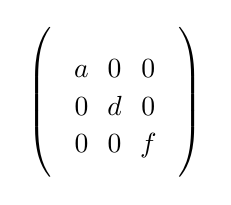
\begin{tikzpicture}[line cap=round]
         \matrix[
            matrix of math nodes, ampersand replacement=\&,
            left delimiter=(, right delimiter=)
         ]{
            a \& 0 \& 0\\ 
            0 \& d \& 0\\ 
            0 \& 0 \& f\\
         };
      \end{tikzpicture}
      \caption*{\color{DarkBlue1}
      Matrice diagonale}
   \end{subfigure}\quad
   \begin{subfigure}{.3\textwidth}
      \centering
      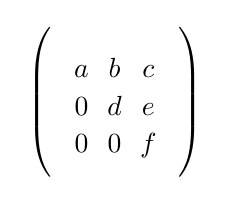
\begin{tikzpicture}[line cap=round]
         \matrix[
            matrix of math nodes, ampersand replacement=\&,
            left delimiter=(, right delimiter=)
         ]{
            a \& b \& c\\ 
            0 \& d \& e\\ 
            0 \& 0 \& f\\
         };
      \end{tikzpicture}
      \caption*{\color{DarkBlue1}
      Matrice triangulaire supérieure}
   \end{subfigure}\quad
   \begin{subfigure}{.3\textwidth}
      \centering
      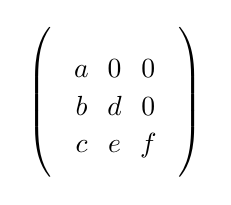
\begin{tikzpicture}[line cap=round]
         \matrix[
            matrix of math nodes, ampersand replacement=\&,
            left delimiter=(, right delimiter=)
         ]{
            a \& 0 \& 0\\ 
            b \& d \& 0\\ 
            c \& e \& f\\
         };
      \end{tikzpicture}
      \caption*{\color{DarkBlue1}
      Matrice triangulaire inférieure}
   \end{subfigure}
\end{figure}

Puis on a deux types de matrices qui sont liées à la symétrie des coefficients et à \textbf{l'opération de transposition}\footnote[1]{En effet une matrice symétrique est égale à sa transposée et une matrice antisymétrique à \textbf{l'opposée} de sa transposée}:
\begin{figure}[h]
   \color{DarkBlue1}
   \centering
   \begin{subfigure}{.3\textwidth}
      \centering
      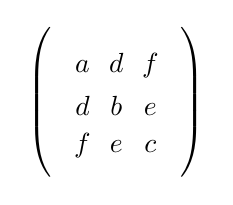
\begin{tikzpicture}[line cap=round]
         \matrix[
            matrix of math nodes, ampersand replacement=\&,
            left delimiter=(, right delimiter=)
         ]{
            a \& d \& f\\ 
            d \& b \& e\\ 
            f \& e \& c\\
         };
      \end{tikzpicture}
      \caption*{\color{DarkBlue1}Matrice symétrique}
   \end{subfigure}\quad
   \begin{subfigure}{.3\textwidth}
      \centering
      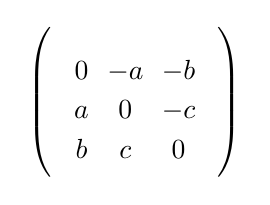
\begin{tikzpicture}[line cap=round]
         \matrix[
            matrix of math nodes, ampersand replacement=\&,
            left delimiter=(, right delimiter=)
         ]{
            0 \& -a \& -b\\ 
            a \& 0 \& -c\\ 
            b \& c \& 0\\
         };
      \end{tikzpicture}
      \caption*{\color{DarkBlue1}Matrice antisymétrique}
   \end{subfigure}
\end{figure}

On a aussi \textbf{les matrices élémentaires} qui sont obtenus par \textbf{opérations élémentaires}\footnote[2]{Voir la partie suivante.} sur la matrice identité:
\begin{figure}[h]
   \color{DarkBlue1}
   \centering
   \begin{subfigure}{.3\textwidth}
      \centering
      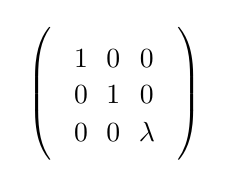
\begin{tikzpicture}[line cap=round]
         \matrix[
            matrix of math nodes, ampersand replacement=\&,
            left delimiter=(, right delimiter=)
         ]{
            1 \& 0 \& 0\\ 
            0 \& 1 \& 0\\ 
            0 \& 0 \& \lambda\\
         };
      \end{tikzpicture}
      \caption*{\color{DarkBlue1}Matrice de dilatation}
   \end{subfigure}\quad
   \begin{subfigure}{.3\textwidth}
      \centering
      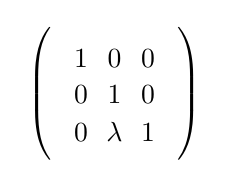
\begin{tikzpicture}[line cap=round]
         \matrix[
            matrix of math nodes, ampersand replacement=\&,
            left delimiter=(, right delimiter=)
         ]{
            1 \& 0 \& 0\\ 
            0 \& 1 \& 0\\ 
            0 \& \lambda\& 1\\
         };
      \end{tikzpicture}
      \caption*{\color{DarkBlue1}Matrice de transvection}
   \end{subfigure}\quad
   \begin{subfigure}{.3\textwidth}
      \centering
      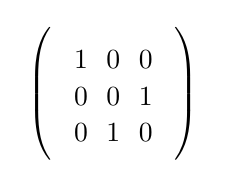
\begin{tikzpicture}[line cap=round]
         \matrix[
            matrix of math nodes, ampersand replacement=\&,
            left delimiter=(, right delimiter=)
         ]{
            1 \& 0 \& 0\\ 
            0 \& 0 \& 1\\ 
            0 \& 1\& 0\\
         };
      \end{tikzpicture}
      \caption*{\color{DarkBlue1}Matrice de permutation}
   \end{subfigure}
\end{figure}

Enfin, on a \textbf{les matrices orthogonales} qui sont des matrices telles que leur inverse soit \textbf{leur transposée}, ce sont par exemple les matrices de rotation:
\begin{figure}[H]
   \color{DarkBlue1}
   \centering   
   \begin{subfigure}{.3\textwidth}
      \centering
      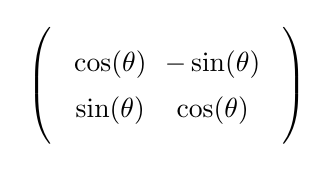
\begin{tikzpicture}[line cap=round]
         \matrix[
            matrix of math nodes, ampersand replacement=\&,
            left delimiter=(, right delimiter=)
         ]{
            \cos(\theta) \& -\sin(\theta)\\ 
            \sin(\theta) \& \cos(\theta) \\
         };
      \end{tikzpicture}
      \caption*{\color{DarkBlue1}Matrice de rotation}
   \end{subfigure}
\end{figure}

\pagebreak
\subsection*{\subsecstyle{Echelonnements \& Calculs{:}}}
\addcontentsline{toc}{subsection}{Echelonnements et calculs}

La théorie permettant de lier matrices, applications linéaires et familles de vecteurs, l'étude des espaces vectoriels engendrés par les colonnes ou les lignes d'une matrice revêt alors une importantce capitale qui est l'objet de cette partie.\<

On appelle \textbf{opérations élémentaires} sur une matrice \(M\), l'une de ces 3 opérations:
\begin{itemize}
   \item Multiplier une colonne par un scalaire
   \item Ajouter une colonnes à une autre
   \item Echanger deux colonnes
\end{itemize}
Il est alors possible de montrer que ces trois opérations préservent \textbf{le sous-espace engendré}\footnote[1]{L'échange ne change évidement rien, et le sous espace engendré ne change pas pas multiplication par un scalaire ou ajout d'un vecteur venant de la famille en question.} par les colonnes de la matrice, donc en particulier \textbf{le rang, le noyau et l'image} sont préservés.\<

Enfin, on appellera \textbf{matrice équivalente} à \(M\) et on notera \(M' \sim M\) la matrice \(M\) à laquelle on a appliqué une ou plusieurs opérations élémentaires.

On dira qu'une matrice \(M\) est \textbf{échelonée} si la matrice obtenue aprés application d'opérations élémentaires est de la forme générale:
\begin{center}
   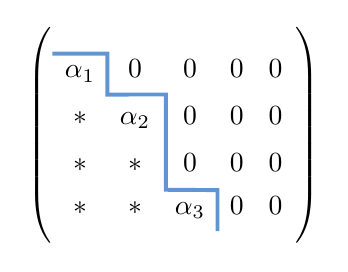
\begin{tikzpicture}[    
      every left delimiter/.style={xshift=.55em},
      every right delimiter/.style={xshift=-.55em}
   ]
      \matrix[
         matrix of math nodes, ampersand replacement=\&,
         left delimiter=(, right delimiter=),  outer sep = 0pt,inner sep=4.5pt
      ] (A) {
         {\alpha_1} \& {0} \& {0} \& {0}\& {0}\\ 
         {*} \& {\alpha_2} \& {0} \& {0}\& {0}\\ 
         {*} \& {*} \& {0} \& {0}\& {0}\\ 
         {*} \& {*} \& {\alpha_3} \& {0}\& {0}\\
      };
      \draw[color=BrightBlue1, line width=0.5mm] (A-1-1.north west) -- (A-1-1.north east) -- (A-1-1.south east) -- (-0.1, 0.57)-- (-0.1, -0.64) -- (A-4-3.north east)-- (A-4-3.south east);

   \end{tikzpicture}   
\end{center}
En d'autres termes, on \textbf{creuse} la matrice pour faire apparaître des zéros sur la partie triangulaire supérieure.\+
Il existe aussi une variante appellé \textbf{échelonnement avec mémorisation}, pour cette variante, on nomme chaque vecteur-colonne de la matrice et on reporte toutes les transformations réalisées sur ces vecteurs. \<

Présentons maintenant les différentes informations que nous pouvons tirer de ces échellonements:

\begin{enumerate}
   \item On peut trés facilement trouver le rang d'une matrice, en effet aprés échelonnement, c'est simplement \textbf{le nombre de colonnes non-nulles} de la matrice. En particulier, il est donc trés facile de montrer qu'une matrice est inversible ou qu'une famille est une base.
   \item On peut trouver une base d'un sous-espace engendré par une famille, pour cela on échelonne la matrice de cette famille, l'ensemble des colonnes non nulles consitue une base du sous-espace initial.
   \item On peut trouver un supplémentaire d'une famille, on échelonne la matrice de la famille, et on complète la matrice par des vecteurs de la base canonique\footnote[2]{Ou alors de telle sorte que la matrice reste échelonnée.}, ces vecteurs formeront alors un supplémentaire.
   \item On peut trouver les équations cartésiennes d'un sous-espace engendré par une famille, pour cela on augmente la matrice de la famille par une matrice d'indéterminées, et on échelonne. Alors la dernière colonne fournira les equations cartésiennes du sous-espace.
   \item On peut trouver le \textbf{noyau, l'image} d'une matrice, gràce à la variante \textbf{avec mémorisation}, alors les colonnes nulles aprés échelonnement permettent d'en déduire des vecteurs envoyés du noyau, et les colonnes non-nulles constituent une base de l'image (voir l'exemple ci-aprés).
\end{enumerate}
Il peut être utile de noter que fondamentalement, on peut à la fois échelonner \textbf{sur les colonnes} ou sur \textbf{les lignes}. En effet, le rang est invariant par transposition, on aurait tout aussi bien pu développer des opération élémentaires sur les lignes, et les résultats seraient équivalents.

\pagebreak

Soit \(M = (C_1, C_2, C_3) = \begin{pmatrix} 1 & 2 & 1\\ 3 & 4 & 2\\ 5 & 6 & 3\end{pmatrix}\), nous allons présenter quelques exemples:
\begin{itemize}
   \item Cherchons le rang de la matrice, on a:
   \[
      M = \begin{pmatrix} 1 & 2 & 1\\ 3 & 4 & 2\\ 5 & 6 & 3\end{pmatrix} \sim  \begin{pmatrix} 1 & 0 & 0\\ 3 & 2 & 2\\ 5 & 4 & 4\end{pmatrix} \sim  \begin{pmatrix} 1 & 0 & 0\\ 3 & 2 & 0\\ 5 & 4 & 0\end{pmatrix} \sim  \begin{pmatrix} 1 & 0\\ 3 & 2\\ 5 & 4\end{pmatrix}
   \]
   La matrice est échelonnée sur \(2\) colonnes, donc son rang est \(2\). En particulier, \((C_1, C_2, C_3)\) n'est pas une base de \(\R^3\), la matrice (donc l'endomorphisme associé) n'est pas inversible.
   \item Cherchons un sous-espace supplémentaire à \((C_1, C_2, C_3)\) en reprenant l'échelonnement ci-dessus, on a simplement à rajouter des colonnes à \(M\) de sorte qu'elle soit échelonnée sur 3 colonnes, par exemple:
   \[
      M' = \begin{pmatrix} 1 & 0 & 0\\ 3 & 2 & 0\\ 5 & 4 & 1\end{pmatrix}
   \]
   Et donc le sous-espace engendré par le vecteur \((0, 0, 1)\) est bien un supplémentaire de l'espace des colonnes.
   \item Cherchons des équations cartésiennes du sous-espace des colonnes, on a:
   \[
      M = \begin{pmatrix} 1 & 2 & 1 & x\\ 3 & 4 & 2 & y\\ 5 & 6 & 3 &z\end{pmatrix} \sim  \begin{pmatrix} 1 & 0 & 0 & 0\\ 3 & 2 & 2 & y-3x\\ 5 & 4 & 4 & z-5x\end{pmatrix} \sim  \begin{pmatrix} 1 & 0 & 0 & 0\\ 3 & 2 & 0 & 0\\ 5 & 4 & x - 2y + z & 0\end{pmatrix}\sim  \begin{pmatrix} 1 & 0 & 0\\ 3 & 2 & 0\\ 5 & 4 & x - 2y + z\end{pmatrix}
   \]
   Alors l'équation cartésienne du sous-espace des colonnes est \(x - 2y + z = 0\).
   \item Cherchons le noyau et l'image de l'endomorphisme représenté par \(M\), on doit utiliser la mémorisation, ie:
   \[
      M = \begin{blockarray}{ccc} C_1 & C_2 & C_3 \\\begin{block}{(ccc)} 1 & 2 & 1\\3 & 4 & 2\\5 & 6 & 3\\\end{block}\end{blockarray} 
      \sim
      \begin{blockarray}{ccc} C_1 & C_2-2C_1 & 2C_3 - 2C_1 \\\begin{block}{(ccc)} 1 & 0 & 0\\3 & 2 & 2\\5 & 4 & 4\\\end{block}\end{blockarray} 
      \sim
      \begin{blockarray}{ccc} C_1 & C_2-2C_1 & 2C_3 - C_2 \\\begin{block}{(ccc)} 1 & 0 & 0\\3 & 2 & 0\\5 & 4 & 0\\\end{block}\end{blockarray} 
   \]
   On en conclut qu'une base de l'image est \([(1, 3, 5), (0, 2, 4)]\).\+
   Le noyau est de dimension 1 et par la mémorisation, une combinaison linéaire nulle est \(0C_1-C_2+2C_3\), le vecteur \((0, -1, 2)\) est bien dans le noyau et est donc une base du noyau.

\end{itemize}\<
\chapter*{\chapterstyle{III --- Déterminant}} % Fini 99%
\addcontentsline{toc}{section}{Déterminant}

Soit \(A = (a_{i,j})\) une matrice carrée de taille \(n\), nous cherchons à définir une application \(\phi: \mathcal{M}_n(\K) \longrightarrow \R\) telle que:
\[
   A \in \text{GL}_n(\K) \Longleftrightarrow \phi(A) = 0
\]
\subsection*{\subsecstyle{Définition{:}}}
\addcontentsline{toc}{subsection}{Définition}

On peut alors montrer\footnote[1]{Particulièrement difficile..} qu'une telle application existe qu'on appellera \textbf{déterminant}, qu'on note \(|A|\) et qu'on définit alors par récurrence:
\begin{itemize}
   \item Si \(n = 1\) alors \(|(a)| = a \) 
   \item Sinon \(|A| := a_{1, 1}|A_{1, 1}| - a_{1, 2}|A_{1, 2}| + \ldots + (-1)^{n+1}a_{1, n}|A_{1, n}|\)
\end{itemize}
Où la notation \(A_{1, 1}\) signifie la matrice \(A\) à laquelle on a retiré la première ligne et la première colonne. \<

Cette opération s'appelle aussi \textbf{développement selon la première ligne} du déterminant, elle se comprends visuellement par:
\[
   |A| = \begin{vmatrix} a & b & c \\ d & e & f \\ g & h & i \end{vmatrix} = 
   a \begin{vmatrix} \square & \square & \square \\ \square & e & f \\ \square & h & i \end{vmatrix} - 
   b \begin{vmatrix} \square & \square & \square \\ d & \square & f \\ g & \square & i \end{vmatrix} + 
   c \begin{vmatrix} \square & \square & \square \\ d & e & \square \\ g & h & \square \end{vmatrix}   
\]
On peut ainsi \textbf{développer le déterminant} selon n'importe quelle ligne ou colonne en suivant cette règle. On régresse ainsi vers des déterminants de plus petite taille, et aprés plusieurs étapes, vers un réel.

\subsection*{\subsecstyle{Propriétés{:}}}
\addcontentsline{toc}{subsection}{Propriétés}

On peut montrer que cette application est \textbf{une forme multilinéaire alternée} en les colonnes ou lignes de la matrice, en particulier, on a les propriétés suivantes:
\begin{itemize}
   \item Ajouter à une colonne une combinaison linéaire \textbf{des autres colonnes} ne change pas le déterminant.
   \item Echanger deux colonnes d'une matrice change le signe du determinant.
   \item Si deux colonnes sont égales ou qu'une des colonnes est nulle, le déterminant est nul.
\end{itemize}
En outre la multilinéarité sur les colonnes ou lignes implique:
\customBox{width=3cm}{
   \(|\lambda A| = \lambda^n |A|\)
}
Et on peut aussi montrer que le déterminant est multiplicatif, ie:
\customBox{width=4cm}{
   \(|A \times B| = |A|\times|B|\)
}

Si on considère une famille \(\Fam = (e_1 , \ldots, e_n)\) de vecteurs de coordonées \((C_1, \ldots, C_n)\) dans une certaine base \(\mathscr{B}\), alors on peut définir le déterminant \textbf{d'une famille de vecteurs} dans cette base par:
\[
   |\Fam|_{\mathscr{B}} = |(C_1, \ldots, C_n)|
\]
\begin{center}
   \textit{Le déterminant d'une famille par rapport à \(\mathscr{B}\) est alors simplement le déterminant de la matrice construite avec les coordonées de ses vecteurs dans la base \(\mathscr{B}\).}
\end{center}

Soit deux bases \(\mathscr{B, B'}\), on pourrait alors considèrer \textbf{l'effet d'un changement de base} sur un tel déterminant et on a alors:
\customBox{width=5cm}{
   \(
      |\Fam|_{\mathscr{B'}} = |\Fam|_{\mathscr{B}} \times |\mathscr{B'}|_{\mathscr{B}}
   \)
}

\subsection*{\subsecstyle{Cofacteurs{:}}}
\addcontentsline{toc}{subsection}{Cofacteurs}

Reprenons en simplifant la définition donnée plus haut du développement selon la première ligne:
\[
   |A| := a_{1, 1}|A_{1, 1}| - a_{1, 2}|A_{1, 2}| + \ldots + (-1)^{n+1}a_{1, n}|A_{1, n}| = \sum_{j=1}^{n}a_{1, j}(-1)^{j+1}|A_{1, j}|
\]
On appelle alors \textbf{cofacteur} de l'élément \(a_{i, j}\) le scalaire:
\customBox{width=5cm}{
   \(
      \text{cof}(a_{i, j}) := (-1)^{j+i}|A_{i, j}|
   \)
}   
Intuitivement en reprenant la visualisation exposée plus haut:
\[
   a \begin{vmatrix} \square & \square & \square \\ \square & \color{BrightRed1}e & \color{BrightRed1}f \\ \square & \color{BrightRed1}h & \color{BrightRed1}i \end{vmatrix} - 
   b \begin{vmatrix} \square & \square & \square \\ \color{BrightRed1}d & \square & \color{BrightRed1}f \\ \color{BrightRed1}g & \square & \color{BrightRed1}i \end{vmatrix} + 
   c \begin{vmatrix} \square & \square & \square \\ \color{BrightRed1}d & \color{BrightRed1}e & \square \\ \color{BrightRed1}g & \color{BrightRed1}h & \square \end{vmatrix}  
\]
Ce sont simplement les déterminants mineurs que l'on calcule à chaque itération \textbf{en tenant compte du signe qui précède le coefficient}.\+
En pratique pour trouver le signe du cofacteur, on ne calcule pas \((-1)^{i + j}\), mais on le détermine par \textbf{la règle de l'échiquier} qu'on peut se représenter comme suit:
\[
   \begin{vmatrix} + & - & + & - & \ldots \\ - & + & - & + &\ldots \\ + & - & + & - &\ldots \\ \vdots & \vdots & \vdots & \vdots \\\end{vmatrix}
\]

\underline{Exemple:} Pour \(\begin{pmatrix}
   1 & 2 & 3 \\ 4 & 5 & 6 \\ 7 & 8 & 9
\end{pmatrix}\), le cofacteur du coefficient en position \((1, 2)\) est 
\(- \begin{vmatrix} 4 & 6 \\ 7 & 9\end{vmatrix} \)

\subsection*{\subsecstyle{Comatrice{:}}}
\addcontentsline{toc}{subsection}{Comatrice}

On peut alors définir \textbf{la comatrice} d'une matrice \(A\) donnée, c'est en fait simplement \textbf{la matrice des cofacteurs} de \(A\), ie le terme en position \((i, j)\) de la comatrice est exactement le cofacteur de l'élement en position \((i, j)\). \<

L'intérêt principal de la comatrice est de calculer l'inverse de matrices inversibles, en effet, on peut montrer l'identité:
\[
   A \times \text{com}(A)^{\top} = |A|I_n   
\]
Et en particulier si le déterminant est non-nul (donc si \(A\) est inversible), on a:
\customBox{width=4.5cm}{
   \[
      A^{-1} = \frac{1}{|A|}\text{com}(A)^{\top}  
   \]
}   
Cette formule est néanmoins particulièrement inexploitable pour \(n > 3\) du fait de la quantité de calcul à réaliser.

\subsection*{\subsecstyle{Formules de Cramer{:}}}
\addcontentsline{toc}{subsection}{Formules de Cramer}

On considère un systême linéaire de \(n\) équations à \(n\) inconnues, alors on peut l'écrire matriciellement sous la forme:
\[
   AX = B   
\]
Pour \(A \in \mathcal{M}_n(\K)\), \(X\) un vecteur indéterminé, et \(B\) le vecteur fixé du second membre des équations.
\pagebreak

Un tel système est dit \textbf{système de Cramer} si la matrice \(A\) est inversible, il possède alors une unique solution qui s'écrit matriciellement \(X = A^{-1}B\). \<

Alors on montre que sa i-ème inconnue \(x_i\) (et par suite la solution tout entière X = \((x_1, \ldots, x_n)\)) est donnée par:
\customBox{width=2.5cm}{
   \[
      x_i = \frac{|A_i|}{|A|}
   \]
} 
Dans laquelle \(A_i\) désigne la matrice obtenue en remplaçant la i-ème colonne de \(A\) par le second membre \(B\)\<

\underline{Exemple:}
\[
   \begin{cases} 
      x + 4y + 8z = 2 \\
      2x + 5y + 8z = 2 \\
      3x + 6y + 9z = 3 \\
   \end{cases}   \Longleftrightarrow 
   \begin{pmatrix}
      1 & 4 & 8 \\
      2 & 5 & 8 \\
      3 & 6 & 9
   \end{pmatrix} 
   \begin{pmatrix}
      x \\
      y \\
      z  
   \end{pmatrix} =
   \begin{pmatrix}
      2 \\
      2 \\
      3  
   \end{pmatrix}
\]
Alors on a:
\[
   y = \frac{
      \begin{vmatrix}
         1 & \color{BrightRed1} 2 & 8 \\
         2 & \color{BrightRed1} 2 & 8  \\
         3 & \color{BrightRed1} 3 & 9
      \end{vmatrix}
   }{|A|} = \frac{6}{-3} = -2
\]

\subsection*{\subsecstyle{Volume orienté{:}}}
\addcontentsline{toc}{subsection}{Volume orienté}

Le déterminant admet un interprétation géométrique intéressante liée au concept d'aire, de volumes, et d'hypervolumes de manière générale. \<

Considérons le cas simple d'une base \(\mathscr{B} = (e_1, e_2)\) de vecteurs de \(\R^2\), alors le déterminant de cette base correspond \textbf{à l'aire algébrique\footnote[2]{C'est une aire ``signée'', ie l'aire géométrique est donc la valeur absolue de cette aire algébrique.} du parallélogramme formé par les deux vecteurs}, ie:
\begin{center}
   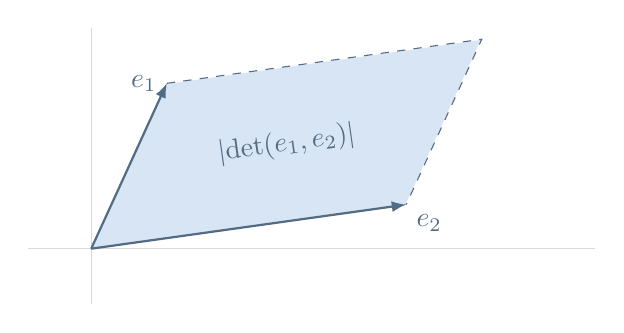
\begin{tikzpicture}[xscale=1.6, yscale=1.4]
      \draw[black!15] (-0.5,0) -- (4,0);
      \draw[black!15] (0, -0.5) -- (0,2);

      \draw[color=black!0, fill=BrightBlue1!25] (0,0) -- (0.6, 1.5) -- (3.1, 1.9) -- (2.5, 0.4);

      \draw node[color=DarkBlue1, rotate=8] at (1.55, 0.95) {$|\text{det}(e_1, e_2)|$};

      \draw[-latex, color=DarkBlue1, thick] (0, 0) -- (0.6, 1.5) node[left] {$e_1$};
      \draw[-latex, color=DarkBlue1, thick] (0, 0) -- (2.5, 0.4) node[below right] {$e_2$};

      \draw[color=DarkBlue1, dashed] (0.6, 1.5) -- (3.1, 1.9)-- (2.5, 0.4);


   \end{tikzpicture}
\end{center}
Plus généralement, le déterminant d'une famille de \(n\) vecteurs est \textbf{l'hypervolume algébrique} du parallélotope formé par ces \(n\) vecteurs.\<

\subsection*{\subsecstyle{Orientation{:}}}
On peut alors définir \textbf{l'orientation d'un espace vectoriel}, en effet, on dira que deux bases \(\mathscr{B}, \mathscr{B'}\) ont meme orientation si et seulement si:
\[
   \text{det}(\text{Pass}(\mathscr{B}, \mathscr{B'})) > 0
\]
Si on fixe alors une base orientée canoniquement, on qualifie son orientation (et celles de toutes les bases de meme orientation) de \textbf{directe} et les bases d'orientation opposée sont alors d'orientation \textbf{indirecte}.\<

\underline{Exemple:} Dans le cas de \(\R^n\), la base canonique est la base qui, par convention, est d'orientation directe.\<

On peut alors définir le \textbf{groupe spécial linéaire}, noté SL\((\R)\), des endomorphismes qui respectent l'orientation de l'espace.
\chapter*{\chapterstyle{III --- Dualité}}
\addcontentsline{toc}{section}{Dualité}
On définit dans ce chapitre une notion fondamentale en algèbre linéaire, trés liée à celle de produit scalaire, qui est celle \textbf{d'espace dual} d'un espace vectoriel \(E\), qu'on notera \(E^*\) et qu'on définit par:
\begin{center}
   \textbf{L'espace dual d'un espace vectoriel est l'ensemble des formes linéaires sur cet espace.}
\end{center}
Attention, on parle ici de dual \textbf{algébrique}, on peut aussi définir un dual \textbf{topologique} en requierant que les formes linéaires considérées soit continues. Dans la plupart des exemples, on considèrera \(E = \R^2\) et donc par exemple un élément de \(E^*\) est:
\[
   \phi : (x, y) \mapsto 2x + y   
\]
Dans toute la suite, on se placera dans un espace \(E\) de dimension finie\footnote[1]{Tout ce qui suit est en général faux en dimension infinie, l'idée prinicipale étant qu'en dimension infinie, des considérations topologiques sont \textbf{nécéssaires}.}

\subsection*{\subsecstyle{Notations{:}}}
On introduit de nouvelles notations pratique, tout d'abord on utilisera souvent la notation \textbf{delta de Kronecker} qui pour tout \(n, m \in \N\) donne:
\[
   \begin{cases}
      \delta_{n}^m = 1 \text{ si } n = m\\
      \delta_{n}^m = 0 \text{ sinon }
   \end{cases}
\]

\subsection*{\subsecstyle{Propriétés{:}}}
On souhaite caractériser la forme d'une forme linéaire \(\phi\) de l'espace dual. On a directement par linéarité que:
\[
   \forall x \in E \; ; \; \phi(x) = \phi\left(\sum_{i}x^ie_i\right) = \sum_{i}x^i\phi(e_i)  
\]
Donc en particulier, on a que évidemment que \(\phi\) est caractérisée par ses images des vecteurs de base, et réciproquement si une application \(\phi'\) est telle que \(\phi = \sum_{i}x_ia_i\), alors \(\phi'\) est une forme linéaire sur \(E\).

\subsection*{\subsecstyle{Base duale{:}}}
En dimension finie, on a alors le théorème fondamental suivant:
\begin{center}
   \textbf{L'espace vectoriel et son dual sont isomorphes.}
\end{center}
En effet, on a tout d'abord égalité des dimensions\footnote[2]{Car \(\dim\mathcal{L}(E, F) = \dim\mathcal{L}(E)\dim\mathcal{L}(F)\)}. Fixons une base \(\mathscr{B} = (e_1, \ldots, e_n)\) de \(E\), alors si on considère la famille de formes linéaires suivantes:
\[
   \begin{aligned}
      e_i^* : E &\longrightarrow \R \\
      \sum_{i}x^ie_i &\longmapsto x_i
   \end{aligned}
\]
Alors elle forme alors une base de \(E^*\) qu'on appelera \textbf{base duale} de \(\mathscr{B}\) et qu'on notera \(\mathscr{B}^*\).
\begin{center}
   \textit{C'est une famille de projections qui a chaque vecteur associe la coordonée correspondante.}
\end{center}
Elle vérifie en outre la relation suivante:
\[
   e_i^*(e_j) = \delta_{i}^j
\]

\subsection*{\subsecstyle{Base antéduale{:}}}
On considère alors le problème inverse, et on se donne une base \(\mathscr{B} = (\phi_1, \ldots, \phi_n)\) du dual de \(E\), alors il existe une unique base \((e_1, \ldots, e_n)\) de \(E\) telle que:
\[
   \forall i \in \inticc{1}{n} \; ; \; \phi_i = e_i^*   
\] 
Ou dit autrement il existe une base \(\mathscr{C}\) de \(E\) telle que \(\mathscr{C}^* = \mathscr{B}\).

\subsection*{\subsecstyle{Hyperplans{:}}}
On rapelle alors que d'aprés le cours de première année, on appelle hyperplan tout sous-espace dont le supplémentaire est une droite, on peut alors caractériser les hyperplans en termes de formes linéaires par la proposition suivante:
\begin{center}
   \textbf{Les hyperplans sont exactements les noyaux de formes linéaires.}
\end{center}

\subsection*{\subsecstyle{Vecteurs covariants et contravariants{:}}}
On deux bases \( \mathscr{C}, \mathscr{B}\) de \(E\) et un vecteur \(u\) de coordonées respectives \(U, U'\), on a la propriété de changement de base suivante pour des notations évidentes:
\[
   U' = P^{-1}U
\]
On voit alors ici que les coordonées aprés le changement de base dépendent de \textbf{l'inverse de la matrice de passage}. On dira dans ce cas qu'un vecteur est \textbf{contravariant par rapport aux bases de \(E\)}.\<

Maintenant on considère un vecteur \(u \in E^*\), alors on peut calculer les bases duales \(\mathscr{C}^*, \mathscr{B}^*\) et utiliser la même formule pour montrer que pour des notations évidentes on a:
\[
   U' = \text{Pass}(\mathscr{B}^*, \mathscr{C}^*)U
\]
Or, on peut alors montrer la propriété suivante fondamentale suivante:
\[
   \text{Pass}(\mathscr{B}^*, \mathscr{C}^*) = {}^tP
\]
En particulier on se ramène alors à une matrice de passage entre les bases de \(E\) et on a alors la formule de changement de base suivantes (pour les coordonées placées en ligne):
\[
   {}^tU' = {}^tUP
\]
On voit alors ici que les coordonées aprés le changement de base (en ligne) dépendent de \textbf{la matrice de passage}. On dira dans ce cas qu'un vecteur est \textbf{covariant par rapport aux bases de \(E\)}. Finalement moralement on a les formules de changement de bases suivantes:

\begin{itemize}
   \item Si \(X, Y\) sont des vecteurs : \(Y = P^{-1}X\)
   \item Si \(X, Y\) sont des covecteurs : \({}^tY = {}^tXP\)
\end{itemize}
\begin{center}
   \textbf{La notion de vecteurs contravariants et covariants est centrale en algèbre multilinéaire, elle permet la définition d'objets généraux appelés tenseurs qui généralisent ce concept.}
\end{center}

\chapter*{\chapterstyle{III --- Introduction à la réduction}}
\addcontentsline{toc}{section}{Introduction à la réduction}
Dans ce chapitre, nous étudirons un domaine vaste de l'algèbre linéaire appellé \textbf{réduction des endormorphismes}.\+
En effet, sous une forme quelconque un endomorphisme représenté par une matrice présente plusieurs problèmes:
\begin{align*}
   &\bullet \;\; \text{Il est couteux de calculer les puissances d'une matrice quelconque.} \\
   &\bullet \;\; \text{Une représentation quelconque donne peu d'informations sur l'endomorphisme.}
\end{align*}
L'objectif sera donc de réduire (comprendre simplifier) la représentation de l'endormorphisme, et de le représenter par une matrice plus simple. \<

Soit \(f \in \mathcal{L}(E)\) et une famille \((E_i)\) de sous-espaces \textbf{supplémentaires}\footnote[1]{Comme tout sous-espace admet un supplémentaire (théorème de la base incomplète), on peut définir une base adaptée à \textbf{un seul} sous-espace comme étant une base adaptée à la somme directe de ce sous-espace et de son supplémentaire, qui revient à compléter la base en une base de \(E\).}, alors on peut construire une base \(\mathcal{B}\) dite \textbf{base adaptée à la décomposition} en concaténant des bases respectives des \(E_i\).

\subsection*{\subsecstyle{Elements Propres {:}}}
Soit \(\lambda \in \R\), on dit que \(\lambda\) est une \textbf{valeur propre}\footnote[2]{On appelle \textbf{specte}, noté Sp\((f)\) l'ensemble des valeurs propres de \(f\).} de l'endomorphisme \(f\) si et seulement si il existe un vecteur non-nul \(u \in E\) tel que:
\customBox{width=2.5cm}{
   \(f(u) = \lambda u\)
}
On dira alors qu'un tel vecteur est \textbf{vecteur propre} de l'endomorphisme et on appelle \textbf{sous-espace propre} associé à la valeur propre \(\lambda\) l'ensemble des vecteurs propres associés, qu'on note \(E_\lambda\) dont on déduit une expression\footnote[3]{Directement d'après la définition d'un vecteur propre associé à \(\lambda\).}:
\customBox{width=5cm}{
   \(E_\lambda = \text{Ker}(f - \lambda \text{Id})\)
}
Enfin, on peut montrer une propriété trés importante pour la suite:
\customBox{width=10cm}{
   Toute somme de sous-espaces propres est \textbf{directe}.
}
\begin{center}
   \textit{L'image des sous-espaces propres par l'endomorphisme se réduit à une homotéthie de rapport la valeur propre.}
\end{center}

\subsection*{\subsecstyle{Sous-Espaces Stables {:}}}
On dit que \(F\) est \textbf{stable par l'endormorphisme} si et seulement si:
\customBox{width=2.5cm}{
   \(f(F) \subseteq F\)
}
On considère maintant une base de \(F\) qu'on compléte en une base de \(E\) via le théorème de la base incomplète, alors dans une telle base, l'endormorphisme est représenté par la matrice par blocs:
\[
   \left(\begin{array}{c|c}
      A & B\\
      \hline\\[-1.7\medskipamount]
      0 & C
   \end{array}\right)
\]
\pagebreak

Plus généralement, si on a une famille \((E_i)\) de sous-espaces \textbf{stables et supplémentaires}, ie \(E = \bigoplus_{i \in \N} E_i\), et \(\mathcal{B}\) est une base adaptée à cette décomposition, alors dans cette base, \(f\) est représentée par la matrice diagonale par blocs:
\[
   \left(\begin{array}{ccc}
      A_1 & {} & {}\\
      {} & \ddots & {}\\
      {} & {} & A_n\\
   \end{array}\right)
\]
On remarque donc que la stabilité des sous-espaces nous permet de reprénsenter notre transformation de manière plus simple, en particulier, on peut alors montrer une propriété fondamentale:
\customBox{width=10cm}{
   \textbf{Tout les sous-espaces propres sont stables.}
}

\subsection*{\subsecstyle{Polynôme caractéristique {:}}}
On peut montrer\footnote[1]{\(E_\lambda\) est un noyau, il suffit de caractériser le fait qu'il soit non vide en termes de la bijectivité d'un certain endomorphisme.} que \(\lambda\) est valeur propre si et seulement si:
\begin{align*}
   E_\lambda \neq \bigl\{0_E\bigl\} \Longleftrightarrow \text{det}(f - \lambda \text{Id}) = 0
\end{align*}
On définit alors le \textbf{polynôme caractéristique} d'un endormorphisme par:
\customBox{width=5cm}{
   \(P_f=\text{det}(f - X \text{Id})\)
}
En particulier, on peut donc montrer que:
\customBox{width=15cm}{
   \textbf{Les valeurs propres sont exactement les racines du polynôme caractéristique.}
}
Ceci nous donne donc une méthode systématique pour trouver les valeurs propres d'un endomorphisme. En particulier, on peut alors montrer les identités suivantes, utiles dans la recherche de valeurs propres:
\begin{align*}
   &\bullet \;\; \text{La somme des valeurs propres est égale à \textbf{la trace de la matrice}.} \\
   &\bullet \;\; \text{Le produit des valeurs propres est égale au \textbf{déterminant de la matrice}.}
\end{align*}

\subsection*{\subsecstyle{Diagonalisation {:}}}
Les endomorphismes qu'on peut représenter le plus simplement sont ceux qui ceux réduisent (dans une base bien choisie) à une homotéthie des vecteurs de la base. On dira alors que ces endomorphismes sont \textbf{diagonalisables}, formellement:
\customBox{width=16.5cm}{
   Un endormorphisme est diagonalisable si il existe une base de \(E\) constituée de vecteurs propres de \(f\).
}
De manière équivalente:
\customBox{width=16cm}{
   Un endormorphisme est diagonalisable si ses matrices sont semblables à une matrice diagonale.
}

\underline{Exemple:} Soit \(f\) un tel endormorphisme de \(\R^3\) et \((e_{\lambda_1}, e_{\lambda_2}, e_{\lambda_3})\) des tels vecteurs propres, alors dans cette base, \(f\) est représenté par la matrice:
\[
   D = \left(\begin{array}{ccc}
      \lambda_1 & {} & {}\\
      {} & \lambda_2 & {}\\
      {} & {} & \lambda_3
   \end{array}\right) 
\]
Ou encore si \(A\) est la matrice de \(f\) dans la base canonique, alors \(A = PDP^{-1}\) avec:
\[
   P = ([e_{\lambda_1}]_\mathscr{C}, [e_{\lambda_2}]_\mathscr{C}, [e_{\lambda_3}]_\mathscr{C}) \text{ et } D = \left(\begin{array}{ccc}
      \lambda_1 & {} & {}\\
      {} & \lambda_2 & {}\\
      {} & {} & \lambda_3
   \end{array}\right) 
\]
\begin{center}
   \textit{Diagonaliser un endomorphisme revient à \textbf{décomposer l'espace en somme directe de droites stables}.
   }
\end{center}
\pagebreak

\subsection*{\subsecstyle{Critères de diagonalisabilité {:}}}
On sait qu'un endomorphisme \(f\) est diagonalisable si et seulement si il admet une base de vecteurs propres, alors on peut montrer\footnote[1]{En effet, si tel est le cas, alors il suffit de prendre une base pour chaque \(E_\lambda\) (qui est bien constituée de vecteurs propres par définition), et de les concaténer pour obtenir une base de \(E\) constituée de vecteurs propres.} que \(f\) est diagonalisable si et seulement si:
\customBox{width=4cm}{
   \(
      E = \bigoplus_{\lambda \in \text{Sp}(f)} E_\lambda  
   \)
}
En particulier on remarque alors que montrer la supplémentarité revient à montrer que \textbf{la somme des dimensions des sous-espaces propres est égale à la dimension totale} car toute somme de sous-espaces propres est directe.\<

On peut alors montrer que si \(\lambda\) est une valeur propre de multiplicité \(\alpha\) pour le polynome caractéristique, alors:
\[
   1 \leq \text{dim}(E_\lambda) \leq \alpha   
\]
On a alors le théorème fondamental suivant:
\begin{center}
   \textbf{Un endomorphisme est diagonalisable si et seulement si son polynôme est scindé sur \(\K\) et que la dimension de chaque sous-espace propre est égale à la multiplicité de la valeur propre associée}.
\end{center}
On peut donc étudier si un endormorphisme est diagonalisable en calculant les valeurs propres et les dimensions des sous-espaces propres associés, ce qui revient à un calcul de polynôme caractéristique suivi de calculs de noyau.

\underline{Exemple:} Diagonalisons la matrice \(A = \left(\begin{array}{ccc}
   1 & 1 & 1\\
   2 & 2 & 2\\
   3 & 3 & 3
\end{array}\right) \)\< 

On peut calculer \(P_A = \text{det}(A - XI_3) = X^2(X-6)\), on a alors deux sous-espaces propres, \(E_0\) et \(E_6\) et on sait que \(E_0\) est de dimension \(1\), il suffit alors de vérifier que \(E_6\) est bien de dimension \(2\) pour conclure que \(\sum \dim(E_\lambda) = \dim(E)\) et donc que la matrice est diagonalisable.\<

Pour trouver une base de vecteurs propres, il suffit alors de trouver une base de \(E_0, E_6\) et de la concaténer en une base de \(E\).
\chapter*{\chapterstyle{III --- Polynomes d'endomorphismes}}
\addcontentsline{toc}{section}{Polynomes d'endomorphismes}
L'objet principal de ce chapitre est l'étude des polynômes d'endomorphismes et de matrices, en effet, les matrices est les endomorphismes formant une algèbre, on peut en calculer des puissances, des sommes, et effectuer un multiplication externe, on peut donc définir des \textbf{polynômes de matrices/d'endomorphismes}, en effet si on a \(P = \sum_{k=0}^{n} a_kX^k \in \K[X]\) et \(u\) un endomorphisme, on définit alors:
\[
   P(u) = \sum_{k=0}^{n}a_k u^k  
\]
\subsection*{\subsecstyle{Propriétés {:}}}
On définit alors un \textbf{morphisme d'algèbre} pour un endomorphisme donné par:
\[
   \begin{aligned}
      \phi_u:  \K[X] &\longrightarrow \mathcal{L}(E) \\
      P &\longmapsto P(u)
   \end{aligned}
\]
En particulier, on a donc \(PQ(u) = P(u) \circ Q(u)\), on peut alors en déduire la proposition suivante:
\begin{center}
   \textbf{Deux polynôme d'un même endomorphisme commutent.}
\end{center}
On peut alors montrer que les polynômes d'endomorphismes ont un bon comportement vis-à-vis
des changements de bases, en particulier si \(A = PBP^{-1}\), pour tout polynôme \(Q\), on montre facilement que:
\[
   Q(A) = PQ(B)P^{-1}   
\]
Enfin, on montre aussi que si \(u\) est représenté par \(A\) dans une base, alors \(u^k\) est représenté par \(A^k\) dans cette même base, et donc par linéarité \(P(u)\) est représenté par \(P(A)\) dans cette base. En particulier, le polynôme d'un endomorphisme ne dépends alors par de la représentation choisie.
\subsection*{\subsecstyle{Valeurs propres d'un polynôme d'endomorphisme {:}}}
Pour un endormorphisme \(u\) admettant une valeur propre \(\lambda\) de vecteur propre associé \(v\), on peut alors étudier le lien entre les polynômes d'endomorphisme et les valeurs propres, et en particulier, on peut montre que \(\lambda^k\) est valeur propre de \(u^k\) et donc par linéarité que:
\[
   P(u)(V) = P(\lambda)(V)
\]
Et donc que \(P(\lambda)\) est valeur propre de \(P(u)\).
\subsection*{\subsecstyle{Polynômes annulateurs {:}}}
On considère \(u \in \mathcal{L}(E)\), et on définit l'ensemble des \textbf{annulateurs} de \(u\) par:
\[
   \mathscr{A}_u := \Bigl\{ P \in \K[X] \; ; \; P(u) = 0_{\mathcal{L}(E)} \Bigl\}   
\]
Ce sont l'ensemble des polynômes qui annulent \(u\). On définit de même les polynômes annulateurs de matrices. Une propriété fondamentale est alors que cette ensemble n'est jamais vide\footnote[1]{Il suffit de considèrer la dimension de \(E\), et une famille plus grande que cette dimension, donc liée, et on peut alors trouver un polynôme en \(u\) qui s'annule.}, en effet on a que:
\begin{center}
   \textbf{Tout endormoprhisme admet un polynôme annulateur non-nul.}
\end{center}
On peut alors étudier le lien entre les valeurs propres d'un endomorphisme et ses annulateurs, et on peut alors montrer la propriété suivante:
\[
   \text{Sp}(u) \subseteq \bigl\{ \alpha \in \K \; ; \; P(\alpha) = 0 \bigl\}   
\]
\begin{center}
   \textit{Les seules valeurs propres possibles sont les racines de l'annulateur}.
\end{center}
\pagebreak
Néanmoins il n'y a pas équivalence, plus précisément, si \(A_u \in \mathscr{A}_u\), et si on définit \(Q_u = (X - \lambda_1)\ldots(X - \lambda_k)\) où les \((\lambda_i)\) sont toutes les valeurs propres de \(u\), alors on a:
\customBox{width=4cm}{
   \(
      Q_u \; |\;  A_u   
   \)   
}
\subsection*{\subsecstyle{Polynôme minimal {:}}}
On considère l'ensembe des annulateurs d'un endomorphisme \(u\), alors il est non-vide comme énoncé ci-dessus, et il admet aussi \textbf{un plus petit élément unitaire} (au sens du degré) et il est unique.\<

On appelle alors ce plus petit élément \textbf{le polynôme minimal} de \(u\) qu'on note \(M_u\)
\subsection*{\subsecstyle{Théorème de Cayley-Hamilton {:}}}
On peut alors énoncer le théorème fondamental de la réduction des endormorphismes, ie le \textbf{théorème de Cayley-Hamilton}:
\begin{center}
   \textbf{Le polynôme caractéristique est un annulateur.}
\end{center}
La démonstration, non-triviale, se fait par un argument topologique et par la continuité de la fonction polynôme caractéristique. On a donc la relation avec le polynôme minimal suivante:
\[
   M_u \; | \; P_u   
\]
\subsection*{\subsecstyle{Lemme des noyaux {:}}}
On s'intéresse finalement aux \textbf{noyaux de polynômes d'endomorphismes} pour pouvoir énoncer le dernier théorème de cette partie. On peut tout d'abord montrer facilement le résultat suivant:
\begin{center}
   \textbf{Le noyau d'un polynôme d'endomorphisme est stable par celui-ci.}
\end{center}
Soit \(P, Q\) deux polynômes \textbf{premiers entre eux}, on peut alors montrer\footnote[1]{La démonstration est non-trivial et fait appel à la relation de Bezout pour les polynômes.} le \textbf{lemme des noyaux}, c'est à dire que:
\customBox{width=7cm}{
   \(\Ker{PQ(u)} = \Ker{P(u)} \oplus \Ker{Q(u)}\)
}
En particulier, pour \(P\) un polynôme annulateur de \(u\) qui se décompose en \(P_1, \ldots, P_k\), on a la décomposition suivante de l'espace tout entier:
\[
   E = \bigoplus_{k=1}^n \Ker{P_k(u)}
\]
\subsection*{\subsecstyle{Caractérisations via les annulateurs {:}}}
On peut caractériser la diagonalisabilité via les annulateurs, en effet, on peut montre via le lemme des noyaux qu'on a:
\begin{center}
   \textbf{Un endomorphisme est diagonalisable si et seulement si il admet un annulateur scindé à racines simples}.
\end{center}
On peut aussi caractériser la trigonalisabilité par:
\begin{center}
   \textbf{Un endomorphisme est trigonalisabilité si et seulement si il admet un annulateur scindé}.
\end{center}
\chapter*{\chapterstyle{III --- Trigonalisation}}
\addcontentsline{toc}{section}{Trigonalisation}
Les endomorphismes qu'on ne peut représenter sous forme diagonale nous posent alors problème, on cherche alors dans ce chapitre à mobiliser la théorie des polynômes d'endomorphismes pour comprendre les conditions pour représenter de tels endomorphismes sous une forme plus simple triangulaire, ou sous \textbf{forme de Dunford} qui sera présentée ci-dessous.

\subsection*{\subsecstyle{Critère de trigonalisation {:}}}
On peut montrer le critère suivant:
\begin{center}
   \textbf{Un endomorphisme \(u\) est trigonalisable sur \(\K\) si et seulement si son polynôme caractéristique est scindé sur \(\K\).}
\end{center}
En particulier tout les endormorphismes sont trigonalisables dans \(\C\).\<

Néanmoins, on comprends vite qu'une forme triangulaire quelconque sera peu utile car on ne pourra calculer ses puissances facilement, on peut alors montrer que si \(u\) est trigonalisable, il admet une forme plus simple encore appellée \textbf{forme de Dunford}:
\[
   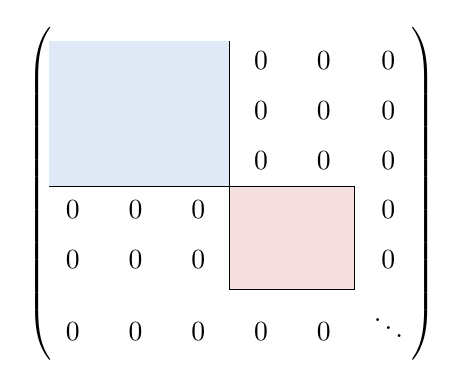
\begin{tikzpicture}[every left delimiter/.style={xshift=2mm},
         every right delimiter/.style={xshift=-2mm}]
      \path (0,0) node (mat) [matrix,matrix of math nodes,left delimiter=(,right delimiter=),column sep=2mm,row sep=1mm]
      {
      |(A)|\lambda_1 & * & * & 0 & 0 & 0\\
      0 & \lambda_1 & * & 0 & 0 & 0\\
      0 & 0 & |(B)|\lambda_1 & 0 & 0 & 0\\
      0 & 0 & 0 & |(C)|\lambda_2 & * & 0\\
      0 & 0 & 0 & 0 & |(D)|\lambda_2 & 0\\
      0 & 0 & 0 & 0 & 0 & |(E)|\ddots \\
      };
      \path 
      (B)--(C) coordinate[midway] (P)
      (D)--(E) coordinate[midway] (Q)
      ;
      \begin{scope}
         \draw[fill=BrightRed1!20] (P) rectangle (Q);
         \fill[BrightBlue1!20] (P) rectangle (A.north west);
         \draw 
         (P)--(P-|A.west) (P)--(P|-A.north);
      \end{scope}
   \end{tikzpicture}
\]
C'est une matrice \textbf{triangulaire par blocs triangulaires}. Et les puissances de telles matrices sont alors facile à calculer via le produit par blocs et le binôme de Newton. En effet chaque bloc et de la forme \(\lambda I_n + N\) avec \(N\) nilpotente, donc le binôme simplifie grandement les calculs.

\subsection*{\subsecstyle{Structure des noyaux itérés {:}}}
Soit \(u\) un endomorphisme, alors on peut montrer que les noyaux des puissances de \(u\) forment la structure suivante:
\[
   \Ker{u} \subsetneq \Ker{u^2} \subsetneq \ldots \subsetneq \Ker{u^k}   
\]
Et cette suite de noyaux itérés est \textbf{stationnaire}, en particulier, si \(u\) est nilpotent, elle est stationnaire et le dernier sous espace est \(E\) tout entier.
\subsection*{\subsecstyle{Sous-espaces caractéristiques {:}}}
Soit \(u\) un endomorphisme de polynôme caractéristique \(P_u = (X - \lambda_1)^{\alpha_1}\ldots(X - \lambda_k)^{\alpha_k}\), alors on appelle \textbf{sous-espace caractéristique} associé à la valeur propre \(\lambda_k\) le sous-espace suivant:
\[
   F_{\lambda_k} = \Ker{(u - \lambda_k\text{Id})^{\alpha_k}}   
\]
On sait que les \((X - \lambda_k)^{\alpha_k}\) sont premiers entre eux, donc d'aprés le théorème de Cayley-Hamilton et le lemme des noyaux, on a:
\[
   E = F_{\lambda_1} \oplus \ldots \oplus F_{\lambda_k}
\]
Et donc en particulier on a \(\dim(F_{\lambda_1}) = \alpha_1\).
\begin{center}
   \textit{Les sous-espaces caractéristiques sont des sous-espaces propres "sympathiques".}
\end{center}
C'est sont aussi des noyaux de polynômes d'endomorphismes donc en particulier, ils sont stables par \(u\). Par ailleurs, d'aprés la structure des noyaux itérés, on a:
\[
   E_{\lambda_k} = \Ker{(u - \lambda_k\text{Id})^1} \subsetneq \Ker{(u - \lambda_k\text{Id})^2} \subsetneq \ldots \subsetneq \Ker{(u - \lambda_k\text{Id})^{\alpha_k}} = F_{\lambda_k}
\]
Ce sont ces sous-espaces qui nous permettront de construire un base de \(E\) dans laquelle \(u\) est représenté par une matrice de Dunford.
\subsection*{\subsecstyle{Trigonalisation de Dunford {:}}}
On peut alors définir une méthode générale de trigonalisation de Dunford, on considère un endomorphisme \(u\) et son polynôme caractéristique, alors on obtient une base de trigonalisation de Dunford par l'algorithme suivant:
\begin{itemize}
   \item Si la dimension du sous-espace propre \(E_\lambda\) est égale à la multiplicité, le bloc associé à \(\lambda\) est diagonal, et la base recherchée est une base du sous-espace propre
   \item Sinon, on calcule une \textbf{base adaptée} aux noyaux itérés \(E_\lambda \subsetneq \Ker{(u - \lambda\text{Id})^2} \subsetneq \ldots \subsetneq F_\lambda\) via le théorème de la base incomplète puis les coordonées de l'image de cette base par \(u\) pour obtenir le bloc associé à \(\lambda\).
\end{itemize}

\underline{Exemple:} Dans toute la suite nous considérerons l'exemple de l'endomorphisme de \(\R^5\) de polynôme caractéristique \(P_u = (X - 2)^2(X - 3)^3\), alors d'après le lemme des noyaux et le théorème de Cayley-Hamilton, on a:
\[
   E = F_2 \oplus F_3 
\]
Les valeurs propres sont \(2, 3\) et on supposera que la première valeur propre est telle que la dimension du sous-espace propre est égale à la multiplicité, alors on trouve aisément une base \(e_1, e_2\) du bloc associé à \(2\), il sera diagonal.\< 

Il nous suffit alors de trouver une base de \(F_3 = \Ker{(u - 3\text{Id})^3}\) qu'on va calculer de la manière suivante:
\begin{itemize}
   \item On calcule une base de \(E_3 = \Ker{u - 3\text{Id}}\)
   \item On la complète en une base de \(\Ker{(u - 3\text{Id})^2}\)
   \item On la complète en une base de \(F_3 = \Ker{(u - 3\text{Id})^3}\)
\end{itemize}
Finalement, on a \(F_3\) de dimension \(3\) et donc une base \(e_3, e_4, e_5\) de \(F_3\). La base finale recherchée est donc \((e_1, e_2, e_3, e_4, e_5)\) et dans cette base la matrice est de la forme:
\[
   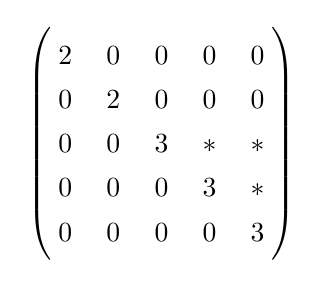
\begin{tikzpicture}[every left delimiter/.style={xshift=2mm},
         every right delimiter/.style={xshift=-2mm}]
      \path (0,0) node (mat) [matrix,matrix of math nodes,left delimiter=(,right delimiter=),column sep=2mm,row sep=1mm]
      {
      2 & 0 & 0 & 0 & 0\\
      0 & 2 & 0 & 0 & 0\\
      0 & 0 & 3 & * & *\\
      0 & 0 & 0 & 3 & *\\
      0 & 0 & 0 & 0 & 3\\
      };
   \end{tikzpicture}
\]
Où les coefficients \(*\) sont donnés par le calcul des cordonnées des images des vecteurs dans la base. 
\chapter*{\chapterstyle{III --- Applications de la réduction}}
\addcontentsline{toc}{section}{Applications de la réduction}
Dans cette dernière partie, on va maintenant pouvoir développer les applications possibles de la réduction dans la résolution de problèmes variés. On considère ici le cas d'une matrice 
\[
   A = \begin{pmatrix}
      2 & 1 & 1 \\
      1 & 2 & 1 \\
      0 & 0 & 3
   \end{pmatrix} = P \begin{pmatrix}
      1 & 0 & 0 \\
      0 & 3 & * \\
      0 & 0 & 3
   \end{pmatrix} P^{-1}
\]
Dans le cas plus simple de matrice diagonalisable, tout les calculs sont plus simples et les mêmes méthodes s'appliquent.

\subsection*{\subsecstyle{Calculs de puissances {:}}}
La première étape pour calculer une puissance de matrice via la réduction est de remarquer que:
\[
   A^k = (PTP^{-1})^k = PT^kP^{-1}   
\]
Or, \(T^k\) se calcule alors par blocs et on a:
\[
   T^k = \begin{pmatrix}
      B_1^k & \\
      & B_2^k \\
   \end{pmatrix} = \begin{pmatrix}
      1 & \\
      & B_2^k \\
   \end{pmatrix}
\]
Et on a alors \(B_2 = 3\text{Id} + N\) avec \(N\) strictement triangulaire donc nilpotente, et donc on calcule facilement sa puissance via le binôme de Newton car Id commute toujours.

\subsection*{\subsecstyle{Suites récurrentes {:}}}
Soit \(3\) suites \(u_n, v_n, w_n\) telles que \(u_1 = 1, v_1 = 1, w_1 = 1\)on considère maintenant le \textbf{système de suites récurrentes} suivant:
\[
   \begin{cases}
      u_{n} = 2u_{n - 1} + v_{n - 1} + w_{n - 1}\\
      v_{n} = u_{n - 1} + 2v_{n - 1} + w_{n - 1}\\
      w_{n} = 3w_{n - 1}\\
   \end{cases}   
\]
On pose alors \(U_n = \begin{pmatrix}
   u_n \\ v_n \\ w_n
\end{pmatrix}\) et le système se réécrit alors sous la forme matricielle suivante:
\[
   U_{n} = AU_{n - 1}   
\]
Par récurrence on trouve alors que \(U_{n} = A^nU_1\), donc en particulier sachant \(U_1\), il nous suffit alors de calculer \(A^k\) comme précédemment ainsi que la matrice de passage et son inverse pour réussir à trouver le terme général de \(u_n, v_n\) et \(w_n\).\<

Plus subtilement, cette méthode s'applique aussi aux suites récurrentes d'ordre multiple, considérons par exemple la suite \(u_n\) de premiers termes \(u_1 = 1\) et \(u_2 = 2\) :
\[
   u_{n} = u_{n - 1} + u_{n - 2}   
\]
En effet si on pose \(U_n = \begin{pmatrix}
   u_{n-2} \\ u_{n-1} \\ u_n
\end{pmatrix}\)
alors on a l'expression matricielle:
\[
   U_{n} = \begin{pmatrix}0 & 1 & 0 \\ 0 & 0 & 1 \\ 0 & 1 & 1\end{pmatrix}U_{n - 1}  
\]
Alors si la matrice est diagonalisable\footnote[1]{La matrice associée à la suite de Fibonacci n'est pas réductible dans \(\R\) donc on ne peut pas trouver une expression de son terme général.}, on peut alors trouver une expression de \(U_n\) en fonction de \(U_0\) et alors une expression de \(u_n\) simplement en fonction de \(n\).
\subsection*{\subsecstyle{Systèmes différentiels {:}}}
On considère trois fonctions réelles \(f, g, h\) de classes \(\mathcal{C}^1\) et on cherche à résoudre le système différentiel suivant:
\[
   \begin{cases}
      f'(x) = 2f(x) + g(x) + h(x)\\
      g'(x) = f(x) + 2g(x) + h(x)\\
      h'(x) = 3h(x)\\
   \end{cases}  
\]
On pose alors \(F(x) = \begin{pmatrix}
   f(x) \\ g(x) \\ h(x)
\end{pmatrix}\) et le système se réécrit alors sous la forme matricielle suivante:
\[
   F'(x) = AF(x) = PTP^{-1}F(x)
\]
On pose alors \(G(x) = P^{-1}F(x) = \begin{pmatrix} g_1(x) \\ g_2(x) \\ g_3(x) \end{pmatrix}\), alors on se ramène à l'équation matricielle suivante:
\[
   G'(x) = TG(x)    
\]
Alors on s'est ramené à un système triangulaire que l'on sait résoudre en partant du bas.\<

On peut donc résoudre pour \(G(x)\), et alors \(F(x)\) est égal à \(PG(x)\) (en utilisant la définition de \(G(x)\)) et on a donc trouvé les fonctions qui satisfont le système. Si on a des conditions initiales, on peut alors résoudre pour trouve l'unique triplet qui le satisfait.

   \pagebreak  
   
   \addcontentsline{toc}{chapter}{Algèbre Bilinéaire} % Reste la compréhension de l'adjoint à trouver, le reste semble nice
   \chapter*{\chapterstyle{V --- Espaces Quadratiques}}
\addcontentsline{toc}{section}{Espaces Quadratiques}
On se donne un espace vectoriel \(E\), on dira que c'est un \textbf{espace quadratique} si et seulement si on peut définir une \textbf{forme bilinéaire symétrique} sur cet espace.\<

Alors on pourra alors définir une \textbf{forme quadratique} sur cet espace qui est une application \(q : E \rightarrow \K\) telle que pour une certaine forme bilinéaire symétrique \(f\), on ait:
\[
   q(x) = f(x, x)   
\]
On appelera alors le membre de droite \textbf{forme polaire} de la forme quadratique \(q\). On remarquera par la suite que moralement ces deux applications s'interpètent de la manière suivante:
\begin{itemize}
   \item Une forme bilinéaire symétrique mesure des "angles" dans l'espace.
   \item Une forme quadratique mesure des "longeurs" dans l'espace.
\end{itemize}
Mais dans le cas général d'un espace quadratique et sans plus d'hypothèses, ces "angles" et "longueurs" ne correspondent pas vraiment aux concepts géométriques que l'on connaît. Tout l'algèbre bilinéaire développée dans ce chapitre peut se résumer à étudier des formes primitives qui par la suite permettront d'axiomatiser la notion de \textbf{produit scalaire} qui incarnera les propriétés géométriques recherchées. 

\subsection*{\subsecstyle{Formules de polarisation{:}}}
On considère une forme quadratique \(q\) quelconque et on souhaiterait reconstituer la forme polaire de \(q\), alors on peut montrer qu'elle vérifie les \textbf{identités de polarisation} ci-dessous:
\[
   \begin{cases}
      f(x, y) = \frac{1}{4}(q(x + y) - q(x - y))\\
      f(x, y) = \frac{1}{2}(q(x + y) - q(x) - q(y))\\
   \end{cases}   
\]
C'est identités se retrouvent aisément en considérant la forme quadratique triviale sur \(\R\) associée à \(f(x, y) = xy\) qui est donc \(q(x) = x^2\).
\subsection*{\subsecstyle{Expression matricielle{:}}}
En dimension finie, on peut représenter les vecteurs \(x, y \in E\) dans une base \(\mathscr{B} = (e_i)\), on peut alors développer par bilinéarité et symétrie pour obtenir:
\customBox{width=5.5cm}{
   \[
      f(x, y) = \sum_{1 \leq i, j \leq n}x_iy_j f(e_i, e_j)   
   \]
}
En particulier on peut alors remarquer que la forme bilinéaire est parfaitement déterminée par la donnée des \(n^2\) images des paires des vecteurs de la base. En particulier, en notant \(X, Y\) les vecteurs colonnes des coordonées de \(x, y\) dans la base, alors on peut montrer qu'il existe une matrice \(A\) telle que:
\customBox{width = 4cm}{
   \(
      [f(x,y)]^\mathscr{B} = X^\top A Y
   \)
}
Et cette matrice est alors de la forme suivante:
\[
   (a_{i, j}) = f(e_i, e_j)
\]
En particulier cette matrice est symétrique et représente parfaitement la forme bilinéaire symétrique et la forme quadratique\footnote[1]{Il suffit de calculer les coordonées de \(f(x, x)\) pour le voir, on trouve alors qu'elle sont égales à \(X^\top A X\)}.
\subsection*{\subsecstyle{Règle du dédoublement{:}}}
Supposont que l'on connaisse une expression analytique de \(q(x)\) dans une base \((e_i, \ldots, e_n)\), on a alors:
\[
   q(x) = \sum_{1 \leq i, j \leq n} x_ix_j f(x_i, x_j) = \sum_{1 \leq i, j \leq n} x_ix_j b_{i, j}
\]
Et donc par symétrique du produit, on peut alors retrouver la matrice \(A = (a_{i,j})\) de \(q\) par la règle dite du \textbf{dédoublement des termes}, ie:
\[
   \begin{cases}
      a_{i,j} &= b_{i, j} \text{ si } i = j\\
      a_{i,j} &= \frac{1}{2} b_{i, j} \text{ si } i \neq j\\
   \end{cases}   
\]
\uline{Exemple:} On considère la forme quadratique suivante sur \(\R^2\):
\[
   q(x, y) = 3x^2 + 5y^2 + 8xy
\]
Alors la règle du dédoublement des termes nous donne que la matrice de \(q\) dans la base canonique est:
\[
   M = \begin{pmatrix}
      3 & 4 \\
      4 & 5
   \end{pmatrix}   
\]
\subsection*{\subsecstyle{Orthogonalité{:}}}
On peut alors définir une notion d'orthogonalité\footnote[1]{\textbf{Attention:} Pour l'instant ceci n'est \textbf{pas} une notion géométrique, mais purement algébrique.} pour la forme bilinéaire \(f\), qu'on appelera \(f\)-orthogonalité, et on dira alors: 
\begin{center}
   \textbf{Deux vecteurs sont \(f\)-orthogonaux si et seulement si \(f(x, y) = 0\).}
\end{center}
On notera alors \(x \perp y\). On peut alors définir le concept de famille \(f\)-orthogonale, ainsi que le concept de base \(f\)-orthogonale, comme une famille telle que tout les vecteurs soient deux à deux orthogonaux.\<

\textbf{Attention:} Dans le cas général, une famille orthogonale n'est pas forcément libre ! Il suffit de considérer \(q(x, y) = x^2\) et la famille \((0, 1), (0, 1)\). C'est une nouvelle conséquence du fait que cette notion d'orthogonalité n'est \textbf{pas géométrique}.
\subsection*{\subsecstyle{Orthogonal d'une partie{:}}}
Soit \(A\) une partie de \(E\), alors on peut définir l'orthogonal de \(A\) comme \textbf{le sous-espace vectoriel} défini par:
\customBox{width=6cm}{
   \(A^\perp := \bigl\{ u \in E \; ; \; \forall v \in A \, , \, u \perp v  \bigl\}\) 
}
En dimension finie, on a alors une base \((e_1, \ldots, e_n)\) de \(F\) et on a la caractérisation suivante:
\customBox{width=7cm}{
   \(F^\perp := \bigl\{ u \in E \; ; \; \forall i \in \inticc{1}{n} \, , \, u \perp e_i  \bigl\}\)
}
On peut alors montrer les propriétés suivantes pour l'application qui a une partie associe son orthogonal:
\begin{itemize}
   \item La décroissance du passage à l'orthogonal.
   \item L'inclusion de la partie dans son double orthogonal.
\end{itemize}
\subsection*{\subsecstyle{Noyau{:}}}
Pour une forme bilinéaire quelconque, il est possible que l'ensemble \(E^\perp\) soit non-trivial, on appelle alors cet ensemble \textbf{noyau} de la forme bilinéaire, cette dénomination\footnote[2]{\textbf{Attention:} Ici on montre que le noyau de la forme bilinéaire est défini par le noyau de l'application linéaire associée à sa matrice, c'est non-trivial.} venant de la raison ci-dessous, pour \(M\) la matrice de la forme bilinéaire:
\[
   E^\perp = \ker(M)
\]
\pagebreak

Avec ces définitions il est alors possible de montrer un analogue à la \textbf{formule du rang}:
\[
   \dim(\Ker{q}) + \dim(\Im{q}) = \dim(E)
\]
Si ce noyau est trivial, on dira alors que la forme bilinéaire est \textbf{non-dégénérée} et en \textbf{dimension finie} on a alors les égalités suivantes:
\[
   \begin{cases}
      \dim(F^\perp) + \dim(F) = \dim(E)\\
      F = F^{\perp^\perp}
   \end{cases}
\]
Attention, ici il est important de noter que même pour une forme non-dégénérée, on n'a \textbf{pas la supplémentarité à priori}.
\subsection*{\subsecstyle{Cône isotrope{:}}}
Pour une forme bilinéaire quelconque, il est aussi possible que l'ensemble \(\{ x \in E ; f(x, x) = q(x) = 0\}\) soit non-trivial, ici il s'agit des vecteurs dont la "longueur" est nulle, on appelera alors ces vecteurs \textbf{vecteurs isotropes}. On a alors directement l'inclusion suivant:
\begin{center}
   \textbf{Le noyau est inclu dans le cône isotrope.}
\end{center}
Si le cône isotrope est trivial, alors on dira que la forme est \textbf{définie}.
\subsection*{\subsecstyle{Cas particulier des formes réelles{:}}}
Soit \(f\) une forme bilinéaire symétrique réelle, alors on classifie ces formes par:
\begin{itemize}
   \item Si \(\forall x \in E, f(x, x) \geq 0\), on dira que la forme est \textbf{positive}.
   \item Si \(\forall x \in E, f(x, x) \leq 0\), on dira que la forme est \textbf{négative}.
\end{itemize}
\subsection*{\subsecstyle{Réduction{:}}}
On cherche maintenant à trouver une base \(\mathscr{B}\) de \(E\) telle que l'expression de \(f(x, y)\) soit plus simple, en particulier on essaye de trouver une base telle que sa matrice soit \textbf{diagonale}, et on peut alors facilement montrer que c'est équivalent à \textbf{chercher une base \(f\)-orthogonale}. On a alors dans une telle base:
\[
   q(x) = \sum_{i\in I}q(e_i)x_i^2 = \sum_{i \in I}q(e_i)e_i^*(x)^2
\]
On peut montrer le théorème suivant:
\begin{center}
   \textbf{Il existe des formes linéaires indépendantes telles que \(q(x) = q(e_1)l_1(x)^2+\ldots+q(e_n)l_n(x)^2\)}
\end{center}
En particulier, ce théorème se démontre de manière constructive via un algorithme qui nous permettra de réduire tout forme bilinéaire en somme de carrés de formes linéaires indépendantes, c'est la \textbf{réduction de Gauss}, une fois les formes linéaires explicitées, il faut alors compléter la famille de formes linéaires en une base du dual, et la base orthogonale recherchée sera \textbf{la préduale de cette base}.
\subsection*{\subsecstyle{Algorithme de Gauss{:}}}
On se donne une forme quadratique suivante à décomposer:
\[
   q(x) = \sum_{i, j}c_{i, j}x_ix_j
\]
L'algorithme est récursif et comporte deux cas:
\begin{itemize}
   \item La forme quadratique comporte un terme carré de la forme \(c_{i,i}x_i^2\)
   \item La forme quadratique ne comporte pas de termes carrés de la forme \(c_{i,i}x_i^2\)
\end{itemize}
\pagebreak

Traitons ces deux cas séparément:
\begin{itemize}
   \item Dans le premier cas, on regroupe tout les termes qui comportent le terme carré et on applique la formule \(A^2 + BA = (A + \frac{B}{2})^2 - \frac{B}{2}^2\) ce qui fait apparaître un carré de forme linéaire.
   \item Dans le second cas on regroupe tout les termes qui contiennent deux variables choisies et la formule \(AB = \frac{1}{4}((A + B)^2 - (A - B)^2)\) ce qui fait apparaître des carrés de formes linéaires.
\end{itemize}
\uline{Exemple:} On pose la forme quadratique suivante:
\[
   q(x, y, z, t) = x^2 + 2xy + y^2 - 4yz
\]
On commence par isoler les termes en \(x\) et appliquer la formule du premier cas, on a donc notre premier carré de forme linéaire:
\[
   q(x, y, z, t) = (x^2 + 2xy) +y^2 - 4yz = (x + y)^2 -y^2 + y^2 - 4yz = l_1(x, y, z, t)^2 - 4yz
\]
Maintenant on réapplique l'algorithme à la forme quadratique restante \(\tilde{q}(x, y, z) = -4yz\), on applique la formule du second cas et on a:
\[
   \tilde{q}(x, y, z, t) = -4yz = -((y + z)^2 - (y - z)^2) = -l_2(x, y, z, t)^2 + l_3(x, y, z, t)^2
\]
Finalement on trouve:
\[
   q(x, y, z, t) = l_1(x, y, z, t)^2 - l_2(x, y, z, t)^2 + l_3(x, y, z, t)^2 = (x + y)^2 - (y + z)^2 + (y - z)^2
\]
On a alors trouvé les formes linéaires recherchées \(l_1, l_2, l_3\) et pour trouver une base \(f\)-orthogonale de \(\R^4\), il reste encore la dernière étape:
\begin{center}
   \textbf{On complète \((l_1, l_2, l_3)\) en une base du dual de \(E\) et la base recherchée est alors la préduale de celle-ci.}
\end{center}
\subsection*{\subsecstyle{Signature{:}}}
On définir alors la \textbf{signature d'une forme bilinéaire} comme étant le couple d'entiers \((p, q)\) avec:
\begin{itemize}
   \item L'entier \(p\) est \textbf{le nombre de valeurs propres strictement positives}.
   \item L'entier \(q\) est \textbf{le nombre de valeurs propres strictement négatives}.
\end{itemize}
On peut alors montrer \textbf{la loi d'inertie de Sylvester} et si on a la forme réduite:
\[
   q(x) = \alpha_1l_1(x)^2 + \ldots + \alpha_nl_n(x)^2
\]
Alors on cette loi nous donne que \(p\) est exactement le nombre de coefficients \(\alpha_i\) strictement positifs, et \(q\) le nombre de coefficients négatifs.
\chapter*{\chapterstyle{V --- Espaces Préhilbertiens Réels}}
\addcontentsline{toc}{section}{Espaces Préhilbertiens Réels}
On appelle \textbf{espace préhilbertien réel} un \(\R\)-espace vectoriel muni d'une forme \textbf{bilinéaire symétrique définie et positive}, c'est à dire une forme qui vérifie:

\customBox{width=7cm}{
   \begin{align*}
      &\textbf{Symétrie} &&f(u, v) = f(v, u) \\
      &\textbf{Définie} &&f(u, u) = 0 \implies u = 0 \\
      &\textbf{Positivité} &&f(u, u) \geq 0
   \end{align*}
}   
On dira alors qu'une telle forme est un \textbf{produit scalaire} sur \(E\) et on notera:
\[
   f(x, y) = \dotproduct{x}{y}
\]
Cet espace, qui est un cas particulier d'espace quadratique, est celui où se réalisera la signification \textbf{géométrique} des formes bilinéaires et quadratiques, gràce aux nouvelles contraintes sur ces formes.
\subsection*{\subsecstyle{Exemples {:}}}
\begin{itemize}
   \item On définit sur \(\R^n\) le produit scalaire défini par:
   \[
      \dotproduct{u}{v} = \sum_{k=1}^{n} u_kv_k    
   \]
   \item On définit sur \(\mathcal{C}^1(\icc{0}{1}, \R)\) le produit scalaire défini par:
   \[
      \dotproduct{f}{g} = \int_{0}^{1} f(t)g(t) d t    
   \]
   \item On définit sur \(\R_n[X]\) le produit scalaire défini pour \((x_n)\) \(n + 1\) points fixés par:
   \[
      \dotproduct{P}{Q} = \sum_{k=0}^{n}P(x_k)Q(x_k)
   \]   
   \item On définit sur \(\mathcal{M}_n(\R)\) le produit scalaire défini par:
   \[
      \dotproduct{A}{B} = \text{tr}(A^\top B)
   \]
\end{itemize}
\subsection*{\subsecstyle{Norme {:}}}
A partir de la définition d'un tel espace, on alors montrer que \(\dotproduct{\cdot}{\cdot}\) \textbf{induit une norme} sur \(E\) donnée par la \textbf{forme quadratique associée}:
\customBox{width=5cm}{
   \(
      \forall u \in E \; ; \; \vectNorm{u}^2 = \dotproduct{u}{u}
   \)
}
Cela fait donc de \(E\) un espace vectoriel normé.
\subsection*{\subsecstyle{Angle{:}}}
A partir de ces définitions, on peut alors définir \textbf{l'angle non-orienté} \(\theta \in \icc{0}{\pi}\) entre deux vecteurs \(u, v\) par:
\customBox{width=4.5cm}{
   \[
      \theta := \cos^{-1}{\left(\frac{\dotproduct{u}{v}}{\vectNorm{u}\vectNorm{v}}\right)}   
   \]
}
Ce qui nous permet de caractériser \textbf{l'orthogonalité} du produit scalaire comme un orthogonal \textbf{géométrique}, en effet \(\theta \equiv \frac{\pi}{2}\) dans cette définition ssi \(\dotproduct{u}{v} = 0\)
\begin{center}
   \textit{L'interprétation de cet "angle" ou de "l'orthogonalité" entre deux vecteurs diffère selon le contexte, elle peut alors signifier une corrélation en probabilité, ou un réel angle géométrique dans \(\R^n\) par exemple.}
\end{center}
\subsection*{\subsecstyle{Inégalité de Cauchy-Schwarz{:}}}
Dans tout espace préhilbertien réel, pour tout \(u, v \in E\) on a l'inégalité\footnote[1]{Trés puissante et permet d'obtenir des majorations dans des cas trés variés, la preuve parte de l'étude du polynôme \(P(t) = \vectNorm{x + ty}^2\)} suivante:
\customBox{width=4cm}{
   \(
      |\dotproduct{u}{v}| \leq \vectNorm{u}\,\vectNorm{v}
   \)
}
Avec cas d'égalité quand \(u, v\) sont \textbf{liés}.
\subsection*{\subsecstyle{Formules géométriques{:}}}
Dans tout espace préhilbertien réel, pour tout \(u, v \in E\) on a les identités suivantes:
\begin{itemize}
   \item \textbf{Identité du parallélogramme :} \(\vectNorm{x + y}^2 + \vectNorm{x - y}^2 = 2\vectNorm{x}^2 + 2\vectNorm{y}^2\).

   \item \textbf{Théorème de Pythagore :} \(x \perp y \Longleftrightarrow \vectNorm{x + y}^2 = \vectNorm{x}^2 + \vectNorm{y}^2\).
\end{itemize}
La première caractérise les espaces normés telles que leur norme soit issue d'un produit scalaire.
\subsection*{\subsecstyle{Orthogonalité{:}}}
Dans le cadre des espaces préhilbertiens, l'orthogonal obtient alors une partie des propriétés géométriques intuitives qu'on lui connait, en particulier:
\begin{itemize}
   \item Une famille orthogonale de vecteurs non-nuls est toujours libre.
   \item Une partie et son orthogonal sont toujours en somme directe.
\end{itemize}
Attention dans un espace préhilbertien quelconque, ils ne sont pas toujours supplémentaires, on verra que c'est le cas en dimension finie !
\subsection*{\subsecstyle{Théorème de représentation{:}}}
On se donne un élément \(\phi\) du dual d'un espace préhilbertien alors, dans ce cadre, et même de manière générale dans celui des espaces de Hilbert, on peut montrer \textbf{le théorème de représentation de Riesz} qui caractérise une forme linéaire \(\phi\) par le produit scalaire:
\[
   \exists w \in E \; , \; \forall x \in E \; ; \; \phi(x) = \dotproduct{w}{x}   
\]
Simplement, cela signifie que toute forme linéaire est \textbf{exactement représentée} par le produit scalaire pour un certain vecteur \(w\), en particulier, on a donc une bijection entre \(E\) et son dual.\<

\uline{Exemple}: On prends la forme linéaire \(\phi(x, y ,z) = 5x+4y+3z\) et on munit \(\R^3\) de son produit scalaire canonique, alors pour tout \(u\) on a directement que:
\[
   \phi(u) = \dotproduct{(5, 4, 3)}{u}
\]
\subsection*{\subsecstyle{Transposition{:}}}
On se donne \(f \in \mathcal{L}(E, F)\) représentée par une matrice \(M \in \mathcal{M}_{n, p}(\R)\), alors on définit \textbf{l'application transposée} de \(f\) par:
\[
   \begin{aligned}
      f^\top : F^* &\longrightarrow E^*\\
      \phi &\longmapsto \phi \circ f
   \end{aligned}
\]
On vérifie alors que cette application est bien définie est on a alors la propriété suivante:
\begin{center}
   \textbf{L'application transposée est représentée dans les bases correspondates par la matrice transposée.}
\end{center}
Ce qui donne finalement une interprétation fonctionnelle de la matrice transposée. A FINIR, LA TRANSPOSEE EST EXACTEMENT LADJOINT, LIEN AVEC TOUT LE RESTE A FAIRE, UNIQUE APPLICATION QUI VERFIE <f(x), y> = <x, tf(y)>, DUALITE.
\chapter*{\chapterstyle{V --- Espaces Euclidiens}}
\addcontentsline{toc}{section}{Espaces Euclidiens}
On appelle \textbf{espace euclidien} tout espace préhilbertien réel \textbf{de dimension finie}. Dans toute la suite on prendra \((e_1, \ldots, e_n)\) une base de \(E\).

En particulier, dans une base \textbf{orthonormée}, on a \(\dotproduct{x}{e_i} = x_i\) et donc:
\[
   x = \sum_{k=1}^{n} \dotproduct{x}{e_i}e_i 
\]
\subsection*{\subsecstyle{Orthogonalité{:}}}
En dimension finie, on a finalement l'ensemble des propriétés géométriques de l'orthogonalité qui deviennent vraies, en effet on a::
\customBox{width = 4cm}{
   \(
     F \oplus F^\perp = E 
   \)
}
\begin{center}
   \textit{Tout sous-espace admet un unique supplémentaire orthogonal.}
\end{center}
On peut alors en déduire qu'en dimension finie on a:
\[
   (F^\perp)^\perp = F   
\]
\subsection*{\subsecstyle{Projection orthogonale{:}}}
L'existence d'une unique décomposition nous permet alors de définir \textbf{la projection} sur \(F\) de direction \(F^\perp\) par:
\[
   \text{proj}_F : x = x_F + x_{F^\perp} \mapsto x_F   
\]
En particulier, on en déduit par l'unicité de la décomposition que \(\text{proj}_F(x)\) est \textbf{l'unique vecteur} de \(F\) qui vérifie:
\customBox{width=4cm}{
   \(x - \text{proj}_F(x) \in F^\perp\)
}
Le projeté orthogonal a une signification géométrique importante, en effet on a:
\customBox{width=7cm}{
   \(\vectNorm{x - \text{proj}_F(x)} = \min_{y\in F}(\vectNorm{x - y})\)
}
\begin{center}
   \textit{C'est le vecteur "le plus proche" de \(F\) au sens du produit scalaire utilisé.}
\end{center}
\pagebreak
\subsection*{\subsecstyle{Calcul de projeté orthogonal{:}}}
On considère un sous-espace \(F\) de bases \((e_1, \ldots, e_p)\) et \(x \in E\), on sait d'aprés les propriétés précédentes que \(\text{proj}_F(x)\) est l'unique vecteur de \(F\) tel que \(x - \text{proj}_F(x) \in F^\perp\), ce qui est équivalent à dire que:
\begin{align*}
   &\forall j \in \inticc{1}{p} \; ; \; \dotproduct{x - \text{proj}_F(x)}{e_j} = 0 \Longleftrightarrow \\
   &\forall j \in \inticc{1}{p} \; ; \; \dotproduct{\text{proj}_F(x)}{e_j} = \dotproduct{x}{e_j}
\end{align*}
On raisonne alors par coefficient indeterminés avec l'écriture de \(\text{proj}_F(x) = \sum_{i=1}^{n} \alpha_i e_i\) dans la base de \(F\) pour obtenir l'expression suivante:
\[
   \forall j \in \inticc{1}{p} \; ; \; \sum_{i=1}^{n}\alpha_k \dotproduct{e_i}{e_j} = \dotproduct{x}{e_i}
\] 
Enfin on obtient alors \textbf{le système des équations normales}:
\[
   \begin{cases}
      \alpha_1 \dotproduct{e_1}{e_1} + \alpha_2 \dotproduct{e_2}{e_1} + \ldots + \alpha_p \dotproduct{e_p}{e_1} = \dotproduct{x}{e_1}\\
      \vdots \\
      \alpha_1 \dotproduct{e_1}{e_p} + \alpha_2 \dotproduct{e_2}{e_p} + \ldots + \alpha_p \dotproduct{e_p}{e_p} = \dotproduct{x}{e_p}
   \end{cases} 
\]
Ou de manière équivalente pour \(M\) la matrice du produit scalaire dans la base de \((e_1, \ldots, e_p)\):
\[
   MY = 
   \begin{bmatrix}
      \dotproduct{x}{e_1}\\
      \vdots \\
      \dotproduct{x}{e_p}
   \end{bmatrix}
\]
Dans le cas d'une base \textbf{orthogonale}, le système ci-dessus est beaucoup plus simple, en effet presque tout les produits scalaires sont nuls, et on obtient un système \textbf{diagonal} et donc dans ce cas précis, le projeté orthogonal s'obtient simplement par la formule:
\customBox{width=5cm}{
   \[
      \text{proj}_F(x) = \sum_{k = 1}^{p} \frac{\dotproduct{x}{e_i}}{\dotproduct{e_i}{e_i}}e_i     
   \]
}
Finalement, une remarque importante permet de comprendre la projection sur un sous espace doté d'une base orthogonale, en effet:
\begin{center}
   \textit{Projeter un vecteur sur un sous-espace revient à ajouter les projetés de ce vecteur sur les vecteurs de la base du sous-espace.}
\end{center}
\underline{Exemple:} Le projeté de \(x = (1, 2, 3)\) sur le plan \(\text{Vect}((1, 0, 0), (0, 1, 0))\) est donné par \(\text{proj}_{(1, 0, 0)}(x) + \text{proj}_{(0, 1, 0)}(x)\)
\subsection*{\subsecstyle{Procédé de Gramm-Schmidt{:}}}
Soit \((e_1, \ldots, e_n)\) une base de \(E\), on cherche alors à élaborer un procédé permettant \textbf{d'orthogonaliser cette base} en une base \((\epsilon_1, \ldots, \epsilon_n)\), on pose \(\epsilon_1 = e_1\) et \(H_i = \text{Vect}(e_1, \ldots, e_i)\) et on définit par récurrence:
\customBox{width=12cm}{
   \[
      \epsilon_i = e_i - \text{proj}_{H_{i-1}}(e_i) = e_i - \left(\sum_{k=0}^{i - 1}\text{proj}_{\epsilon_k}(e_k)\right) = e_i - \left(\sum_{k=0}^{i - 1}\frac{\dotproduct{e_i}{\epsilon_i}}{\dotproduct{\epsilon_i}{\epsilon_i}}\epsilon_i \right)
   \]
}

\begin{center}
   \textit{Moralement, on "redresse" chaque vecteur de la base initiale en lui retirant son défaut d'orthogonalité représenté par sa projection sur le sous-espace précédent.}
\end{center}

\chapter*{\chapterstyle{V --- Espaces Hemitiens}}
\addcontentsline{toc}{section}{Espaces Hemitiens}
On peut généraliser la notion de produit scalaire au cas des espaces vectoriels sur \(\C\), en particulier, on dira demandera alors que la forme \(f : H\times H \rightarrow \C\) soit:
\customBox{width=11cm}{
   \begin{align*}
      &\textbf{Linéaire à gauche} &&f(x + \lambda y, z) = f(x, z) + \lambda f(y, z) \\
      &\textbf{Symétrie Hermitienne} && f(u, v) = \overline{f(v, u)} \\
      &\textbf{Définie} &&f(u, u) = 0 \implies u = 0 \\
      &\textbf{Positivité} &&f(u, u) \geq 0
   \end{align*}
}   
On dira alors que \(f\) est un \textbf{produit hermitienne}. Elle est alors dite \textbf{sesquilinéaire} car on a:
\[
   f(x, \lambda y) = \overline{\lambda}f(x, y)
\]
On définit aussi pour toute matrice dans \(\mathcal{M}_n(\C)\), sa \textbf{matrice ajointe} donnée par:
\[
   M^* = {}^t\overline{M}
\]
\subsection*{\subsecstyle{Exemples {:}}}
\begin{itemize}
   \item On définit sur \(\C^n\) le produit hermitien défini par:
   \[
      \dotproduct{u}{v} = \sum_{k=1}^{n} u_k\overline{v_k}   
   \]
   \item On définit sur \(\mathcal{C}^1(\icc{0}{1}, \C)\) le produit hermitien défini par:
   \[
      \dotproduct{f}{g} = \int_{0}^{1} f(t)\overline{g(t)} d t    
   \]
   \item On définit sur \(\C_n[X]\) le produit hermitien défini pour \((x_n)\) \(n + 1\) points fixés par:
   \[
      \dotproduct{P}{Q} = \sum_{k=0}^{n}P(x_k)\overline{Q(x_k)}
   \]   
   \item On définit sur \(\mathcal{M}_n(\C)\) le produit hermitien défini par:
   \[
      \dotproduct{A}{B} = \text{tr}(AB^*)
   \]
\end{itemize}
\subsection*{\subsecstyle{Expression matricielle{:}}}
En dimension finie, on peut représenter les vecteurs \(x, y \in H\) dans une base \(\mathscr{B} = (e_i)\), on peut alors développer par sesquilinéarité:
\customBox{width=5.5cm}{
   \[
      f(x, y) = \sum_{1 \leq i, j \leq n}x_i\overline{y_j} f(e_i, e_j)   
   \]
}
En particulier on peut alors remarquer que la forme bilinéaire est parfaitement déterminée par la donnée des \(n^2\) images des paires des vecteurs de la base. En particulier, en notant \(X, Y\) les vecteurs colonnes des coordonées de \(x, y\) dans la base, alors on peut montrer qu'il existe une matrice \(A\) telle que:
\customBox{width = 4cm}{
   \(
      [f(x,y)]^\mathscr{B} = X^*A Y
   \)
}
Et cette matrice est alors de la forme suivante:
\[
   (a_{i, j}) = f(e_i, e_j)
\]
En particulier cette matrice est égale à son adjointe et représente parfaitement la forme bilinéaire symétrique et la forme quadratique\footnote[1]{Il suffit de calculer les coordonées de \(f(x, x)\) pour le voir, on trouve alors qu'elle sont égales à \(X^* A X\)}.
\subsection*{\subsecstyle{Orthogonalité{:}}}
On peut alors définir la même notion d'orthogonalité et montrer que pour un produit hermitien, toute les propriétés de l'orthogonalité sont conservées sauf une, en effet le \textbf{théorème de Pythagore} n'est plus vrai dans un espace hermitien et on a seulement:
\[
   x \perp y \implies \vectNorm{x + y}^2 = \vectNorm{x}^2 + \vectNorm{y}^2
\]
\subsection*{\subsecstyle{Théorème de représentation{:}}}
On se donne un élément \(\phi\) du dual d'un espace hermitien alors, dans ce cadre, on peut aussi montrer \textbf{le théorème de représentation de Riesz} qui caractérise une forme linéaire \(\phi\) par le produit scalaire:
\[
   \exists w \in H \; , \; \forall x \in H \; ; \; \phi(x) = \dotproduct{x}{w}   
\]
A nouveau, cela signifie que toute forme linéaire est \textbf{exactement représentée} par le produit scalaire pour un certain vecteur \(w\), en particulier, on a donc une bijection entre \(H\) et son dual.\<
\chapter*{\chapterstyle{V --- Opérateurs bornés}}
\addcontentsline{toc}{section}{Opérateurs bornés}
On s'intéresse dans ce chapitre à l'espace des applications linéaires \(\mathcal{L}(E, F)\) où \( E, F \) sont normés. C'est un exemple fondamental en analyse fonctionnelle et en mathématiques en général. On s'intéressera dans ce chapitre à la \textbf{continuité} de ces applications et à poser quelques bases de topologie sur cet espace.
\subsection*{\subsecstyle{Continuité des applications linéaires {:}}}
Soit \(f : E \rightarrow F\) un opérateur linéaire, alors on a le théorème fondamental suivant qui énonce que \(f\) est continue sur son domaine de définition si et seulement si elle vérifie une des conditions équivalentes suivantes:
\begin{itemize}
   \item Elle est continue en 0.
   \item Elle est bornée sur la boule unité.
   \item Elle est uniformément continue.
   \item Elle est lipschitzienne.
\end{itemize}
On dira alors que l'opérateur est \textbf{borné}. Muni des ces équivalences, on peut démontrer la propriétés fondamentale suivante:
\begin{center}
   \textbf{En dimension finie, tout les opérateurs linéaires sont bornés.}
\end{center}
\subsection*{\subsecstyle{Normes d'opérateur {:}}}
On peut munir \( \mathcal{L}(E) \) lui même d'une norme appelée \textbf{norme d'opérateur} d'un opérateur \(f\) par la quantité suivante:
\[
   \opNorm{f} = \inf \left\{ K \; ; \; \forall x \in E \; \vectNorm{f(x)} \leq K \right\} = \sup_{\vectNorm{x} = 1} \vectNorm{f(x)}
\]
En outre si \( E \) est de dimension finie, par l'isomorphisme usuel entre l'espace des application linéaires et celui des matrices, on définit de même la \textbf{norme d'opérateur d'une matrice} par:
\[
   \opNorm{M} = \inf \left\{ K \; ; \; \forall x \in \mathcal{M}_n(\K) \; \vectNorm{MX} \leq K \right\} = \sup_{\vectNorm{X} = 1} \vectNorm{MX}
\]
On peut alors caractériser la continuité d'un opérateur par le fait que sa norme d'opérateur soit \textbf{finie}.
\subsection*{\subsecstyle{Normes matricielles {:}}}
On appelle \textbf{norme matricielle} toute norme sur un espace de matrice qui est aussi une \textbf{norme d'algèbre}, ie telle que:
\[
   \vectNorm{AB} \leq \vectNorm{A}\vectNorm{B}
\]
Par exemple, la norme de Frobenius est une norme matricielle. On a alors la propriété\footnote[1]{Pour montrer ceci il faut remarquer que pour tout \(x \in E\), on a \(\vectNorm{f(x)} = \opNorm{f}\vectNorm{x}\).} suivante:
\begin{center}
   \textbf{Toute norme d'opérateur est une norme matricielle.}
\end{center}
\subsection*{\subsecstyle{Normes usuelles {:}}}
On peut alors chercher à savoir à quoi correspondent les normes d'opérateurs induites par les normes usuelles, on peut montrer qu'elles vérifient:
\begin{itemize}
   \item La norme 1: \(\opNorm{A}_{1} = \max_{1 \leq j \leq n} \sum_{1 \leq i \leq n} |a_{i,j}|\), c'est le \textbf{maximum de la somme des colonnes.}
   \item La norme infinie: \(\opNorm{A}_{\infty} = \max_{1 \leq i \leq n} \sum_{1 \leq j \leq n} |a_{i,j}|\), c'est le \textbf{maximum de la somme des lignes.}
   \item La norme 2: \(\opNorm{A}_{2} = \sqrt{\rho({}^tAA)}\) où \(\rho(M)\) est le \textbf{rayon spectral} de \(M\).
\end{itemize}

On peut alors chercher à savoir à quoi correspondent les normes d'opérateurs induites par les normes usuelles, on peut montrer qu'elles vérifient:
\begin{itemize}
   \item La norme 1: \(\opNorm{A}_{1} = \max_{1 \leq j \leq n} \sum_{1 \leq i \leq n} |a_{i,j}|\), c'est le \textbf{maximum de la somme des colonnes.}
   \item La norme infinie: \(\opNorm{A}_{\infty} = \max_{1 \leq i \leq n} \sum_{1 \leq j \leq n} |a_{i,j}|\), c'est le \textbf{maximum de la somme des lignes.}
   \item La norme 2: \(\opNorm{A}_{2} = \sqrt{\rho({}^tAA)}\) où \(\rho(M)\) est le \textbf{rayon spectral} de \(M\).
\end{itemize}

\chapter*{\chapterstyle{V --- Espaces de Hilbert}}
\addcontentsline{toc}{section}{Espaces de Hilbert}
Dans ce chapitre avancé, en utilisant les notions définies dans le chapitre de topologie et de théorie de la mesure, on cherche à généraliser la notion \textbf{d'orthogonalité}, de \textbf{de base orthogonale} dans le cadre d'un espace vectoriel de dimension quelconque. Pour ceci, on se donne un espace préhilbertien \( H \) à priori complexe muni de sa forme sesquilinéaire.
\begin{center}
   \textbf{On dire que \( H \) est un espace de Hilbert si il est complet pour la norme induite par le produit scalaire.}
\end{center}
En particulier, les espaces de Hilbert sont donc des espace de Banach. Dans tout la suite, on fixera la semi-linéarité du produit scalaire à gauche.
\subsection*{\subsecstyle{Exemples {:}}}
Les deux exemples canoniques d'espaces de Hilbert sont  les espaces \( \ell^2(\N) \) et \( L^2(\R) \) munis des produits scalaires respectifs suivants:
\[ 
   \dotproduct{u}{v} = \sum_{i \in \N} \overline{u_i}v_i \quad\quad\quad \dotproduct{f}{g} = \int_\R \overline{f}g d\mu
\]
En outre, en utilisant le résultat donnant que tout espace vectoriel de dimension finie est complet, on peut montrer que \( \R^n, \C^n \) et plus généralement que tout les espaces vectoriels de dimension finie sont des espaces de Hilbert pour leurs produits scalaires respectifs.
\subsection*{\subsecstyle{Orthogonalité {:}}}
On généralise alors naturellement la définition de l'orthogonalité à ce cas par:
\[ 
   \forall x, y \in H \; ; \; x \perp y \iff \dotproduct{x}{y} = 0
\]
Cette définition nous permet alors naturellement d'étendre la notion \textbf{famille orthogonale et orthonormale} ainsi que celle \textbf{d'orthogonal d'une partie}. On montre alors la propriétés fondamentale suivante pour l'orthogonal:
\begin{center}
   \textbf{C'est un sous-espace vectoriel fermé.}
\end{center}
En effet, en dimension infinie, les sous-espaces ne sont pas nécessairement fermés (contre-exemple ?). On peut montrer néanmoins que l'orthogonal l'est car il s'exprime comme l'intersection des fermés suivants:
\[ 
   A^\perp = \bigcap \text{Ker}(\dotproduct{x}{\cdot}) 
\]
\subsection*{\subsecstyle{Projection orthogonale {:}}}
On généralise la notion de projection orthogonale du cadre euclidien, et on appelera \textbf{projeté} du point \( x \in H \) sur une partie \( C \) nécéssairement \textbf{convexe et fermée} comme le point \(p_C(x) \in C\) si il existe défini par:
\[ 
   \vectNorm{p_C(x) - x} = \min\left\{ \vectNorm{c - x} \; ; \; c \in C \right\} 
\]
C'est le point de \( C \) à distance minimale avec \( x \). On peut alors montrer qu'un tel projeté \textbf{existe toujours} dans un espace de Hilbert. En outre ce point est caractérisé par le \textbf{lemme de l'angle obtus}, ie c'est l'unique point de \( C \) qui vérifie:
\[ 
   \forall x \in H \; \forall c \in C \; ; \; \text{Re}\left(\dotproduct{x - p_C(x)}{c - p_C(x)}\right) \leq 0 
\]
Ceci signifie alors que, conformément à notre intuition, l'angle entre le segment qui relie \(x\) et \( p_C(x) \) et \( x \) et n'importe quel point de \( C \) est \textbf{toujours obtus}.
\pagebreak
\subsection*{\subsecstyle{Décomposition orthogonale {:}}}
Soit \( F \) un sous-espace vectoriel \textbf{fermé} de \( H \), alors on peut montrer que dans ce cadre, on a la décomposition en somme directe suivante:
\[ 
   H = E \oplus E^\perp 
\]
Alors dans ce cas, on peut définir la projection sur chaque composante, elle est \textbf{linéaire et idempotente}, et dans ce cas elle correpond à la projection sur une partie définie plus haut. On aussi la propriété suivante du double ortogonal:
\[ 
   A^{\perp\perp} = \text{adh}(\text{Vect}(A))
\]
\subsection*{\subsecstyle{Familles totales {:}}}
On se donne une famille \( (e_i)_{i \in I} \), alors on dira que cette famille est \textbf{totale} si et seulement si on a:
\[ 
   \text{adh}\left(\text{Vect}(e_i)\right) = H  
\]
Ce concept nous permettra par la suite de définir la notion de \textbf{base orthogonale}. Plus généralement on dira qu'une partie \( A \) est totale si et seulement si \( \text{adh}\left(\text{Vect}(A)\right) = H \). On peut alors caractériser les parties totales par:
\begin{center}
   \( A \) est \textbf{totale} \( \iff A^\perp = \left\{ 0 \right\} \)
\end{center}
\uline{Exemple:} La famille \( (x^n)_{n \in \N} \) est \textbf{totale} dans l'ensemble des fonctions continues sur un segment, c'est le \textbf{théorème de Weierstrass}.

\subsection*{\subsecstyle{Théorème de Pythagore {:}}}
On se donne une famille dénombrable orthogonale \( (e_i)_{i \in D} \), alors on peut montrer la propriété suivante:
\[ 
   (e_i)_{i \in D} \text{ est \textbf{sommable}} \iff (\vectNorm{e_i})_{i \in D} \in \ell^2(D)
\]
Et dans ce cas on a le \textbf{théorème de Pythagore}:
\[ 
   \vectNorm{ \sum e_i }^2 = \sum \vectNorm{e_i}^2
\]
\subsection*{\subsecstyle{Bases Hilbertiennes {:}}}
On peut alors définir le concept de \textbf{base Hilbertienne} d'un espace de Hilbert \( H \), et on dira qu'une famille \( (e_i)_{i \in D} \) dénombrable est une \textbf{base de Hilbert} de \( H \) si et seulement si:
\begin{itemize}
   \item C'est une \textbf{famille orthogonale}.
   \item C'est une \textbf{famille totale}.
\end{itemize}
Un espace de Hilbert qui admet un partie dénombrable dense admet une base de Hilbert et on dira alors qu'il est \textbf{séparable}. On peut alors montrer les propriétés suivantes:
\begin{itemize}
   \item \textbf{Décomposition:} Si \( x \in H \), alors on peut montrer que la famille \( (\dotproduct{e_i}{x}e_i)_{i \in D} \) est sommable et que:
   \[ 
      x = \sum_{i \in D}\dotproduct{e_i}{x}e_i
   \]
   \item \textbf{Egalité de Parseval:} Par Pythagore on a alors:
   \[ 
      \vectNorm{x}^2 = \sum_{i \in D} \left|\dotproduct{e_i}{x}\right|^2
   \]
   \item \textbf{Isomorphisme des coordonées:} Il existe alors un isomorphisme qui à chaque vecteur lui associe ses coordonées:
   \[ 
      \begin{aligned}
         \phi : H &\longrightarrow \ell^2(D) \\
         x &\longmapsto \left(\dotproduct{e_i}{x}\right)_{i \in D}
      \end{aligned}
   \]
\end{itemize}
Ce théorème est le théorème fondamental des espaces de Hilbert et permet alors d'identifier tout espace de Hilbert via ses coordonées à \( \ell^2(D) \). C'est ce théorème qui donnera naissance à \textbf{l'analyse harmonique} et la théorie des séries et transformées de Fourier que l'on verra au chapitre de théorie de la mesure.
\chapter*{\chapterstyle{V --- Endomorphismes Remarquables}}
\addcontentsline{toc}{section}{Endomorphismes Euclidiens}
Aprés avoir défini les espaces euclidiens et hermitiens, on cherche maintenant à s'intéresser aux endomorphismes qui on des propriétés intéressantes en regard du produit scalaire, on sera alors amené à les définir et les étudier. Dans tout la suite, le corps de base peut être \(\K = \R\) ou \(\K = \C\) et l'espace est muni d'un produit scalaire correspondant.
\subsection*{\subsecstyle{Isométries{:}}}
Soit \(f \in \mathcal{L}(E)\), on dira que \(f\) est une \textbf{isométrie} et on note \(f \in O(E)\) si elle \textbf{préserve les angles}, ie si:
\[
   \forall x, y \in E \; ; \; \dotproduct{f(x)}{f(y)} = \dotproduct{x}{y}   
\]
On en déduit directement qu'elle \textbf{préserve aussi les longeurs}\footnote[1]{En particulier, elle est bijective et l'image d'une base orthonormée par une isométrie est toujours orthonormée.}.\<

On peut alors facilement montrer que la composée de deux isométries est une isométrie et que la réciproque l'est aussi. Aussi on peut déduire de la définition les propriétés suivantes:
\[
   \text{Sp}(f) \subseteq \{-1, 1\}   
\]
Ainsi que comme corollaire immédiat:
\[
   \text{det}(f) \in \{-1, 1\}
\]
\subsection*{\subsecstyle{Matrices orthogonales{:}}}
On considère la matrice d'une isométrie dans une base orthonormée, on a alors d'aprés l'expression matricielle du produit scalaire:
\[
   \forall X, Y \in \mathcal{M}_{n, 1}(\K) \; ; \; {}^*(MX)MY = {}^*X{}^*MMY = {}^*XY  
\]
On remarque donc \(f\) est une isométrie si et seulement si sa matrice dans une base orthonormée vérifie \({}^*M = M^{-1}\), on appelera de telles matrices \textbf{matrices unitaires} et on notera ces matrices \(\mathbb{U}_n(\K)\). On peut alors montrer que:
\begin{center}
   \textbf{Les matrices unitaires forment un sous-groupe des matrices inversibles qu'on appelle groupe unitaire.}
\end{center}
En particulier, la matrice de passage entre deux bases orthonormées est une matrice unitaire, et les colonnes d'une telle matrice sont de norme \(1\) et deux à deux orthogonales.
\subsection*{\subsecstyle{Classification des isométries{:}}}
On peut alors classifier les isométries selon leur action sur l'orientation de l'espace:
\begin{itemize}
   \item Si det\(f = 1\) on dira que l'isométrie est directe, et on note l'ensemble de ces isométries SO\((E)\), appelé \textbf{groupe spécial orthogonal}.
   \item Si det\(f = -1\) on dira que l'isométrie est \textbf{indirecte}, mais leur ensemble ne possède pas de structure particulière.
\end{itemize}
Géométriquement, les isométries directes sont donc celles qui préservent l'orientation de l'espace, c'est un sous-groupe du groupe spécial linéaire. Dans le chapitre suivant, on classifie plus précisément les isométries dans le cas d'une petite dimension.
\pagebreak
\subsection*{\subsecstyle{Adjoint d'un endomoprhisme{:}}}
On considère un endomorphisme \(f \in \mathcal{L}(E)\), alors le théorème de représentation de Riesz nous permet d'affirmer qu'il existe un unique endomorphisme \(f^*\) qui vérifie:
\[
   \forall x, y \in E \; ; \; \dotproduct{x}{f(y)} = \dotproduct{f^*(x)}{y}   
\]
On appelle alors cet endomorphisme \textbf{l'adjoint} de \(f\), en particulier si on représente \(f\) par une matrice \(M\) dans une base orthonormée, alors on défini de meme la \textbf{matrice adjointe} de \(M\) par:
\[
   \forall X, Y \in \mathcal{M}_{n, 1}(\R) \; ; \; {}^tXMY = {}^t(M^*X)Y  
\] 
On peut alors facilement montrer que dans le cas présent de matrices, l'adjoint d'un endormorphisme est simplement sa \textbf{transposée}. On verra plus tard que la notion de matrice adjointe est une généralisation de la transposition. On peut alors entrevoir le role spécial que vont jouer les matrices symétriques. A FINIR, LA TRANSPOSEE EST EXACTEMENT LADJOINT, LIEN AVEC TOUT LE RESTE A FAIRE, UNIQUE APPLICATION QUI VERFIE <f(x), y> = <x, tf(y)>, VOIR DUALITE.
\subsection*{\subsecstyle{Endomorphismes auto-adjoints{:}}}
On appelle \textbf{endomorphisme auto-adjoint} (ou encore endomorphisme symétrique) tout endomorphisme qui est égal à son adjoint et on a donc les propriétés suivantes, cas particuliers des définitions ci-dessus:
\[
   \forall x, y \in E \; ; \; \dotproduct{x}{f(y)} = \dotproduct{f(x)}{y}     
\]
Puis matriciellement dans une base ortonormée:
\[
   \forall X, Y \in \mathcal{M}_{n, 1}(\K) \; ; \; {}^*XMY = {}^*(MX)Y  
\]
En particulier dans le cas réel, le fait d'etre auto-adjoint est caractérisé par la propriété simple suivante sur la matrice de l'endomorphisme dans une base orthonormée:
\begin{center}
   \textbf{La matrice de l'endomorphisme est symétrique.}
\end{center}

L'ensemble des endomorphismes auto-adjoints, qu'on note \(\mathcal{S}(E)\) forme un \textbf{sous-espace vectoriel} de \(\mathcal{L}(E)\). Dans la suite on va étudier les propriétés de ces endomorphismes.
\subsection*{\subsecstyle{Théorème Spectral{:}}}
Une propriété fondamentale de ces endomorphismes est la suivante:
\begin{center}
   \textbf{Leurs sous-espaces propres sont orthogonaux.}
\end{center}
On peut alors énoncer un théorème puissant de réduction pour les endomorphismes auto-adjoints, en effet soit \(f\) un tel endomorphisme, alors:
\begin{center}
   \textbf{Il existe une base orthonormée formée de vecteurs propres.}
\end{center}
On a alors le corollaire matriciel pour la matrice \(M\) de \(f\) dans une base, donné par l'existance d'une matrice de passage \(P\) dans le groupe unitaire et d'une matrice diagonale \(D\) telles que:
\[
   M = PDP^*
\]
\subsection*{\subsecstyle{Technique de réduction{:}}}
En particulier, cela nous donne une nouvelle méthode pour réduire les formes bilinéaires, on peut alors diagonaliser dans une base orthonormée et obtenir une base orthogonale pour la forme, en pratique, on effectue l'algorithme suivant:
\begin{itemize}
   \item On trouve une base pour un sous-espace propre.
   \item On l'orthogonalise par Gram-Schmidt. 
\end{itemize}
\subsection*{\subsecstyle{Lien avec les formes bilinéaires{:}}}
On sait donc que les endomorphismes autoadjoints sont représentés par des matrices symétriques, on a donc la propriété suivante:
\begin{center}
   On peut associer \textbf{une forme bilinéaire} symétrique à chaque\footnote[1]{En effet soit \(f \in S(E)\), alors \(\phi(x, y) = \dotproduct{x}{f(y)}\) est une telle forme, et réciproquement Riesz nous donne que \(\phi(x, y) = \dotproduct{x}{f(y)}\) pour une certaine fonction \(f\) qui est alors un endormorphisme autoadjoint.} endomorphisme autoadjoint et \textbf{réciproquement}.
\end{center}
En particulier, les concepts relevant de l'études des formes peuvent alors se transposer dans l'étude des endomorphismes comme les sections suivantes le démontreront.
\subsection*{\subsecstyle{Endomorphismes auto-adjoints positifs{:}}}
On définit alors les endomorphismes autoadjoints \textbf{positifs} qu'on note \(\mathcal{S}^+(E)\) définis par:
\[
   \mathcal{S}^+(E) := \{ f \in \mathcal{S}(E) \; ; \; \text{Sp}(f) \subseteq \R_+ \}  
\]
Cette définition est alors équivalente à la propriété suivante:
\[
   \forall x \in E \; \dotproduct{x}{f(x)} \geq 0
\]
Les matrices symetriques positives définissent alors des formes bilinéaires symétriques positives.
\subsection*{\subsecstyle{Endomorphismes auto-adjoints définis positifs{:}}}
On définit alors enfin les endomorphismes autoadjoints \textbf{définis positifs} qu'on note \(\mathcal{S}^{++}(E)\) définis par:
\[
   \mathcal{S}^{++}(E) := \{ f \in \mathcal{S}(E) \; ; \; \text{Sp}(f) \subseteq \R_+^* \}  
\]
Cette définition est alors équivalente à la propriété suivante:
\[
   \forall x \in E\backslash\{0_E\} \; \dotproduct{x}{f(x)} > 0 
\]
Les matrices symetriques définies positives définissent alors des nouveaux produits scalaires.

\chapter*{\chapterstyle{V --- Isométries en petite dimension}}
\addcontentsline{toc}{section}{Isométries en petite dimension}
On va maintenant étudier le cas particulier des isométries dans le cas de la petite dimension, c'est à dire dans le cas où \(E\) est de dimension \(2\) ou \(3\), on introduira un outil pratique dans ce contexte qui est le \textbf{produit vectoriel} et on classifiera les isométries dans cet espace.

\subsection*{\subsecstyle{Bases directes{:}}}
Pour ce chapitre nous auront besoin du concept \textbf{d'orientation} de l'espace défini dans le chapitre sur les déterminants, en effet on appelera \textbf{base orthonormée directe} toute base ayant même orientation que la base canonique des espaces considérés. Sinon on dira que la base est \textbf{indirecte}.

\subsection*{\subsecstyle{Cas de la dimension \(2\){:}}}
Soit \(\theta\) un réel, on définit les deux matrices orthogonales suivantes:
\[
   R_\theta := \begin{pmatrix}
      \cos(\theta) & -\sin(\theta) \\
      \sin(\theta) & \cos(\theta)
   \end{pmatrix} \quad\quad 
   S_\theta := \begin{pmatrix}
      \cos(\theta) & \sin(\theta) \\
      \sin(\theta) & -\cos(\theta)
   \end{pmatrix}  
\]
On appele alors \(R_\theta\) \textbf{matrice de rotation} d'angle \(\theta\) et \(S_\theta\) est un \textbf{symétrie axiale}\footnote[1]{D'axe la bissectrice de l'angle \(\theta\), faire un dessin.}.
Alors on a le théorème fondamental suivant, pour \(f \in O(E)\) et tout base orthonormée \(\mathscr{B}\), alors il existe \(\theta\) réel tel que:
\[
   [f]_\mathscr{B} \in \bigl\{ R_\theta, S_\theta \bigl\}   
\]
En particulier si \(f\) préserve l'orientation, alors nécéssairement, \(f\) est une \textbf{rotation}. Et donc les matrices de passages entre bases orthonormées directes sont des rotations.\+
En particulier si \(f\) ne préserve pas l'orientation, alors nécéssairement, \(f\) est une \textbf{symétrie axiale}.

\subsection*{\subsecstyle{Cas de la dimension \(3\){:}}}
Dans le cas de la dimension trois, on pose \(\epsilon = \pm 1\) et on définit la matrice suivante:
\[
   M_\theta := \begin{pmatrix}
      \cos(\theta) & -\sin(\theta) & 0\\
      \sin(\theta) & \cos(\theta) & 0\\
      0 & 0 & \epsilon
   \end{pmatrix}   
\]
Alors on a le théorème fondamental suivant, pour \(f \in O(E)\) et tout base orthonormée \textbf{directe} \(\mathscr{B}\), alors il existe \(\theta\) réel tel que:
\[
   [f]_\mathscr{B} = M_\theta 
\]
La classification des isométries dans ce cas est alors plus complexes et repose sur l'étude de la dimension de l'espace des point fixes, qu'on notera \(F\), et on peut alors les classifier selon le tableau\footnote[2]{Le dernier cas peut se ramener par des propriétés trigonométriques au cas d'un rotation, en effet \(-f = R_{\theta + \pi, u}\)} ci-dessous:
\begin{center}
   \renewcommand{\arraystretch}{0.7}
   \begin{tabular}{ c |Sc |Sc |Sc }
      \(\dim(F)\) & Orientation & Matrice & Nature \\ 
      \hline
      3 & Directe & $\begin{pmatrix}1 & 0 & 0\\ 0 & 1 & 0\\ 0 & 0 & 1 \end{pmatrix}$ & Identité\\
      \hline
      2 & Indirecte & \(\begin{pmatrix}1 & 0 & 0\\ 0 & 1 & 0\\ 0 & 0 & -1 \end{pmatrix}\) & Symétrie par rapport à \(F\) \\       
      \hline
      1 & Directe & \(\begin{pmatrix}\cos(\theta) & -\sin(\theta) & 0\\ \sin(\theta) & \cos(\theta) & 0\\ 0 & 0 & 1 \end{pmatrix}\) & Rotation d'axe \(F\) \\ 
      \hline
      0 & Indirecte & \(\begin{pmatrix}\cos(\theta) & -\sin(\theta) & 0\\ \sin(\theta) & \cos(\theta) & 0\\ 0 & 0 & -1 \end{pmatrix}\) & Composée d'une symétrie et d'une rotation d'axe \(F\) 
   \end{tabular}
\end{center}
\pagebreak

\subsection*{\subsecstyle{Produit mixte{:}}}
On considère une famille de vecteurs \(u, v, w\) et deux bases orthonormées directes \(\mathscr{B}, \mathscr{B}'\) de \(E\), alors on a:
\[
   \det([u]_\mathscr{B}, [v]_\mathscr{B}, [w]_\mathscr{B}) = \det([u]_{\mathscr{B}'}, [v]_{\mathscr{B}'}, [w]_{\mathscr{B}'})
\]
On appelle alors le déterminant de cette famille de vecteur \textbf{le produit mixte} de ces trois vecteurs, et on le note:
\[
   \det([u]_\mathscr{B}, [v]_\mathscr{B}, [w]_\mathscr{B}) = [u, v, w]
\]
C'est donc le volume orienté du parallélotope formé par les trois vecteurs.

\subsection*{\subsecstyle{Produit vectoriel{:}}}
On considère une famille de vecteurs \(u, v\), et un vecteur \(x\) quelconque, alors d'aprés le théorème de représentation de Riesz, on a:
\[
   \exists w \in E \; ; \; [u, v, x] = \dotproduct{w}{x}  
\]
On appelle alors ce vecteur \textbf{produit vectoriel} de \(u\) et \(v\) et on le note \(u \times v\). On peut alors à partir des propriétés du determinant, montrer que:
\begin{itemize}
   \item Le produit vectoriel est une application \textbf{bilinéaire altérnée}.
   \item Le produit vectoriel \(u \times v\) est \textbf{orthogonal} à \(u\) et \(v\).
   \item Si \((u, v)\) est une famille orthonormée, \((u, v, u \times v)\) est une base orthonormée directe.
   \item Si \((u, v, w)\) est une base orthonormée directe \(w = u \times v, u = v \times w\) et \(v = w \times u\).
\end{itemize}
Le produit vectoriel est donc un moyen trés pratique de \textbf{construire des bases directes} ou de tester la colinéarité. Analytiquement, on peut le calculer en cordonnées par:
\[
   \begin{pmatrix}
      x_1 \\
      x_2 \\
      x_3  
   \end{pmatrix}\times 
   \begin{pmatrix}
      y_1 \\
      y_2 \\
      y_3  
   \end{pmatrix} = 
   \begin{pmatrix}
      \det\begin{pmatrix}
         x_2 & y_2 \\
         x_3 & y_3 \\
      \end{pmatrix} \\
      -\det\begin{pmatrix}
         x_1 & y_1 \\
         x_3 & y_3 \\
      \end{pmatrix} \\
      \det\begin{pmatrix}
         x_1 & y_1 \\
         x_2 & y_2 \\
      \end{pmatrix}  
   \end{pmatrix}
\]

\subsection*{\subsecstyle{Recherche des éléments caractéristiques{:}}}
Pour réussir à trouver le réel \(\theta\), on utilise alors le faire que dans une base adaptée, on a:
\[
   \text{tr}(f) = 2\cos(\theta) + 1    
\]
Et donc à partir de la trace de la matrice dans une base quelconque, on peut retrouver le cosinus de l'angle \(\theta\) dont il reste à déterminer le sinus pour le caractériser.\<

Arrive alors l'intérêt du produit mixte, en effet, on peut alors montrer que le sinus de l'angle \(\theta\) est du même signe que la quantité ci-dessous, pour \(x\) un vecteur quelconque (souvent \(c_1\)) de notre choix:
\[
   [x, f(x), u]   
\]
Ce qui caractérise alors parfaitement l'isométrie.


   \pagebreak   
   
   \addcontentsline{toc}{chapter}{Topologie} % 95%
   \chapter*{\chapterstyle{V --- Espaces Topologiques}}
\addcontentsline{toc}{section}{Espaces Topologiques}

Soit \(E\) un ensemble non-vide et \(\mathcal{T}\) une ensemble de parties de \(E\) (qu'on appelera \textbf{ouverts}) qui vérifient les propriétés suivantes:
\begin{align*}
   &\bullet \;\;\; \text{\(E\) et \(\emptyset\) sont des ouverts} \\
   &\bullet \;\; \text{Toute union \textbf{quelconque} d'ouverts est un ouvert} \\
   &\bullet \;\; \text{Toute intersection \textbf{finie} d'ouverts est un ouvert}
\end{align*}
Alors le couple \((E, \mathcal{T})\) est appellé \textbf{espace topologique} et \(\mathcal{T}\) est appellée \textbf{topologie} sur \(E\). On définit alors qu'une partie de \(E\) est \textbf{fermée} si son complémentaire est ouvert. On peut alors voir deux exemple triviaux de topologies sur un ensemble:
\begin{itemize}
   \item La \textbf{topologie grossière}, alors les ouverts sont seulements \(E\) et \(\emptyset\).
   \item La \textbf{topologie discrète}, alors les ouverts sont toutes les parties de \(E\).
\end{itemize}
\subsection*{\subsecstyle{Notion de finesse {:}}}
On définit alors une notion de comparaison entre deux topologie \(\mathcal{T}_1\) et \(\mathcal{T}_2\), et on dira que \(\mathcal{T}_2\) est \textbf{plus fine} que \(\mathcal{T}_1\) si et seulement si on a:
\[
   \mathcal{T}_1 \subseteq \mathcal{T}_2
\]
Cela signifie moralement que \(\mathcal{T}_2\) à plus d'ouverts, par exemple la topologie discrète est la plus fine de tout les topologies. Cette relation définit alors \textbf{une relation d'ordre} sur l'ensemble des topologies.
\subsection*{\subsecstyle{Topologie engendrée {:}}}
On se donne \(A\) un ensemble de parties de \(E\), alors on chercher à savoir si il existe une plus petite topologie (au sens de l'inclusion) telle que les éléments de \(A\) soit des ouverts, ie la topologie la moins fine qui contienne \(A\).\<

On peut alors montrer facilement que l'intersection de deux topologies est une topologie et donc que la plus petite topologie qui contienne \(A\) existe, c'est l'intersection de toutes les topologies qui contiennent \(A\). On l'appelera\footnote[2]{On dira aussi que \(A\) est une \textbf{prébase} de cette topologie.} alors \textbf{topologie engendrée} par \(A\).
\subsection*{\subsecstyle{Topologie induite {:}}}
Soit \(A \subseteq E\), alors \(E\) induit une topologie naturelle sur \(A\) appellée \textbf{topologie induite} définie par:
\[
   \mathcal{T}\vert_A := \Bigl\{ A \cap \mathcal{O} \; ; \; \mathcal{O} \in \mathcal{T}_E \Bigl\}  
\]
\begin{center}
   \textit{Un ouvert de \(A\) pour la topologie induite est simplement la trace sur \(A\) des ouverts de \(E\).}
\end{center}
\subsection*{\subsecstyle{Topologie produit {:}}}
Soit \((E_n)\) une famille finie d'espaces topologiques, alors on peut définir une topologie naturelle sur l'espace produit \(\prod E_n\) appellée \textbf{topologie produit} définie par:
\[
   \mathcal{T}_\times := \left\{ \bigcup_I \mathcal{O}_1 \times \ldots \times \mathcal{O}_n \; ; \; (\mathcal{O}_i) \in \mathcal{T}_{E_i} \right\}  
\]
\begin{center}
   \textit{Un ouvert de \(A\) pour la topologie produit est simplement une union quelconque de produits d'ouverts des espaces composantes.}
\end{center}
\pagebreak
\subsection*{\subsecstyle{Topologie quotient {:}}}
Soit \((E, \mathcal{T})\) un espace topologique muni d'une relation d'équivalence et donc d'une \textbf{projection canonique} \(\pi\), alors on peut définir une topologie naturelle sur l'espace quotient \(E/_\sim\) appellée \textbf{topologie quotient} définie par:
\[
   \mathcal{T}_\pi := \left\{ \mathcal{O} \in  E/_\sim\; ; \; \pi^{-1}(\mathcal{O}) \in \mathcal{T}_{E} \right\}  
\]
\begin{center}
   \textit{Un ouvert de \(E/_\sim\) pour la topologie quotient est donc simplement une partie dont la préimage par la projection est un ouvert.}
\end{center}
\subsection*{\subsecstyle{Voisinages {:}}}
On appelle \textbf{voisinage} d'un point \(x \in E\) toute partie \(V\) de \(E\) qui contient un ouvert \(\mathcal{O}\) qui contient \(x\)
On notera \(\mathscr{V}_a\) l'ensemble des voisinages du point \(a\).\<

\underline{Exemple:} \(\ico{-2}{3}\) est un voisinage de \(3\) et de \(0\) pour la topologie classique de \(\R\), engendrée par les intervalles ouverts.
\subsection*{\subsecstyle{Intérieur {:}}}
On définit l'intérieur d'une partie \(A \subseteq E\) comme étant \textbf{le plus grand ouvert contenu dans \(A\)}. En particulier, c'est l'union de tout les ouverts contenus dans \(A\) et on a:
\[
   \text{int}(A) := \bigcup_{\mathcal{O} \subseteq{A}}\mathcal{O}
\]

On peut alors caractériser cet ensemble par une propriété de ses points (appelés points intérieurs):
\[ 
   \text{int}(A) := \left\{ x \in A \; ; \; \exists \mathcal{O}_x \in \mathcal{T}_E \, , \, \mathcal{O}_x \subseteq A \right\}  
\]

L'application qui à toute partie associe son intérieur est idempotente, croissante et anti-extensive\footnote[2]{On appelle anti-extensive une application telle que \(\phi(S) \subseteq S\) (non-standard)} et elle caractérise les ouverts, en effet:
\begin{center}
   Une partie \(A\) est un ouvert si et seulement si \textbf{elle est égale à son intérieur}.
\end{center}
\subsection*{\subsecstyle{Adhérence {:}}}
On définit l'adhérence d'une partie \(A \subseteq E\) comme étant \textbf{le plus petit fermé qui contient \(A\)}. En particulier, c'est l'intersection de tout les fermé qui contiennent \(A\) et on a:
\[
    \text{adh}(A) := \bigcap_{A \subseteq \mathcal{F}}\mathcal{F}
\]
On peut alors caractériser cet ensemble par une propriété de ses points (appelés points adhérents):
\[ 
   \text{adh}(A) := \left\{ x \in A \; ; \; \forall \mathcal{O}_x \in \mathcal{T}_E \, , \, \mathcal{O}_x \cap A \neq \emptyset \right\}  
\]

L'application qui à toute partie associe son adhérence est idempotente, croissante et extensive et elle caractérise les fermés, en effet:
\begin{center}
   Une partie \(A\) est un fermé si et seulement si \textbf{elle est égale à son adhérence}.
\end{center}
\subsection*{\subsecstyle{Frontière {:}}}
On appelle \textbf{frontière} d'une partie \(A\) de \(E\) et on note \(\partial A\) la partie qui vérifie:
\[
   \partial A = \text{adh}{A} \backslash \text{int}{A}
\]
\pagebreak
\subsection*{\subsecstyle{Propriétés {:}}}
Soit \(A \subseteq E\), on peut alors montrer plusieurs propriétés de l'intérieur et de l'adhérence:
\customBox{width=8cm}{
   \( \text{int}(A)^c = \text{adh}(A^c)
   \quad\quad\quad\quad
   \text{adh}(A)^c = \text{int}(A^c)
   \)
}  
On peut aussi montrer les différentes relations suivantes\footnote[1]{Pour comprendre les inclusions strictes, considérer \(\Q\) et \(\R \backslash \Q\) (en tant que parties de \(\R\)).} vis à vis des opérations ensemblistes:
\customBox{width=12cm}{
   \begin{align*}
      \text{int}(A \cap B) = \text{int}(A) \cap \text{int}(B) \quad\quad\quad\quad \text{adh}(A \cup B) = \text{adh}(A) \cup \text{adh}(B) \\
      \text{int}(A \cup B) \supseteq \text{int}(A) \cup \text{int}(B) \quad\quad\quad\quad \text{adh}(A \cap B) \subseteq \text{adh}(A) \cap \text{adh}(B)
   \end{align*}
}  
\subsection*{\subsecstyle{Densité {:}}}
On peut alors définir la notion \textbf{d'espace dense}, on considère \(A \subseteq E\), alors on dira que \(A\) est \textbf{dense dans \(E\)} si et seulement si:
\[
   \text{adh}(A) = E
\]
Et on peut caractériser cette propriété par le fait que tout ouvert non vide de \(E\) coupe \textbf{nécéssairement} \(A\), en d'autres termes:
\[
   \forall \mathcal{O} \in \mathcal{T} \; ; \; \mathcal{O} \cap A \neq \emptyset
\]
\subsection*{\subsecstyle{Séparation {:}}}
Dans de nombreux cas, on exige de la topologie la condition spécifique de \textbf{séparer les points}, ie on souhaite que pour tout points distincts \(x, y\), il existe deux ouverts \textbf{disjoints} qui contiennent respectivement \(x, y\).\<

On apelle \textbf{espace séparé} ou encore \textbf{espace de Hausdorff} un espace topologique qui vérifie cette propriété. La plupart des espaces étudiés en analyse sont des espaces séparés.

\chapter*{\chapterstyle{V --- Espaces Métriques \& Normés}}
\addcontentsline{toc}{section}{Espaces Métriques \& Normés}
Soit \(E\) un ensemble, le cas le plus courant d'espace topologique est le cas des espaces munis d'une application apellée \textbf{distance} ou aussi métrique, c'est une application de \(E \times E\) dans \(\R^+\) qui vérifie:
\begin{align*}
   &\bullet \;\; \text{Elle est \textbf{symétrique}.} \\
   &\bullet \;\; \text{Elle vérifie \textbf{l'inégalité triangulaire}.} \\
   &\bullet \;\; \text{Deux points sont égaux si et seulement si la distance entre ces points est nulle.}
\end{align*}
Alors, l'espace \(E\) muni de cette distance notée \(d\) est alors appelé \textbf{espace métrique}, et on le note \((E, d)\).\<

Si on considére le cas particulier des \textbf{espaces vectoriels normés} (et donc a fortiori des espaces euclidiens), alors la norme induit une distance sur \(E\) et en fait un espace métrique.

\subsection*{\subsecstyle{Topologie métrique {:}}}
On considère un point \(x\) et un réel strictement positif \(r\), alors on définit:
\begin{itemize}
   \item La \textbf{boule ouverte} centrée en  \(x\) et de rayon \(r\) : \(\mathcal{B}(x, r) := \left\{ y \in E \; ; \; d(x, y) < r\right\}\)
   \item La \textbf{boule fermée} centrée en  \(x\) et de rayon \(r\) : \(\mathcal{B}[x, r] := \left\{ y \in E \; ; \; d(x, y) \leq r\right\}\)
\end{itemize}
La distance sur \(E\) induit alors naturellement une topologie sur \(E\) qu'on appelle \textbf{topologie métrique} définie par:
\[
   \mathcal{T}_{d} := \left\{ \bigcup_I \mathcal{B}(x_i, r_i) \; ; \; (x_i, r_i) \in E \times \R_+^* \right\} 
\]
On peut alors facilement montrer que cette ensemble est bien une topologie sur \(E\) et que la topologie induite sur une partie correspond bien à la topologie métrique pour la restriction de la distance.
\subsection*{\subsecstyle{Topologie métrisable {:}}}
On considère un espace topologique \((E, \mathcal{T})\), alors on dira que cet espace est \textbf{métrisable} si et seulement si il existe une distance \(d\) telle que:
\[
   \mathcal{T} = \mathcal{T}_d
\]
Par exemple si on considère un espace muni de la topologie discrète \((E, \mathcal{P}(E))\), alors cet espace topologique est métrisable pour la distance discrète.
\subsection*{\subsecstyle{Topologie produit {:}}}
On considère une famille finie d'espace métriques \((E_n, d_n)\), alors on peut définir une \textbf{distance produit} par:
\[
   d_\infty((x_1, \ldots, x_n), (y_1, \ldots, y_n)) := \max\{d_1(x_1, y_1), \ldots, d_n(x_n, y_n)\}
\]
Alors on montre que la topologie produit coincide avec la topologie métrique pour cette distance. En particulier pour le cas de \(\R^n\), la topologie produit correspond à la topologie métrique pour:
\[
   d_\infty(x, y) = \vectNorm{x - y}_\infty = \max\{|x_1 - y_1|, \ldots, |x_n - y_n|\}
\]
\subsection*{\subsecstyle{Parties bornées et diamètre {:}}}
Soit \( A \subseteq E\), alors on dira que \( A \) est \textbf{bornée} si et seulement si il existe une boule qui contient \( A \), en outre on peut définir le \textbf{diamètre} de la partie \( A \) par:
\[ 
   \delta(A) := \sup \left\{ d(x, y) \; ; \; x, y \in A \right\}  
\]
Et on montre alors qu'une partie est bornée si son diamètre est \textbf{fini}.
\subsection*{\subsecstyle{Equivalences des normes {:}}}
Dans un espace vectoriel normé, on dira alors que deux normes sont \textbf{équivalentes} si il existe deux réel \(c, C\) tel que:
\[
   c\vectNorm{x}_1 \leq \vectNorm{x}_2 \leq C\vectNorm{x}_1
\]
Ici "équivalentes" signifique donc que si il existe une boule pour une norme, alors il existe une boule plus petite et plus grande que celle-ci pour l'autre, en particulier \textbf{les topologies engendrées par ces normes sont égales}\footnote[1]{Néanmoins la réciproque est fausse, si deux topologies métriques sont égales, alors les métriques induisant ces topologies ne sont pas nécessairement équivalentes ! La notion de distances équivalentes est plus forte que celle de topologies équivalentes (égales)}.\+
La notion de norme équivalente permet de montrer la propriété trés utile suivante:
\begin{center}
   Dans un espace vectoriel normé de dimension finie, toutes les normes sont \textbf{équivalentes}.
\end{center}
\subsection*{\subsecstyle{Exemples de boules en dimension finie {:}}}
On considère ici l'espace vectoriel usuel \(\R^2\), on peut alors définir les \textbf{normes de Hölder} définies comme suit:
\customBox{width=6cm}{
   \({||u||}_p = (|u_1|^p + |u_2|^p)^{\frac{1}{p}}\)
}
En particulier pour \(p=2\), on reconnait \textbf{la norme euclidienne standard}. On peut aussi définir \textbf{la norme infini} par:
\customBox{width=6cm}{
   \({||u||}_\infty = \sup\{|u_1|, |u_2|\}\)
}

On peut représenter les boules pour quelques valeurs de \(p\):
\begin{center}
   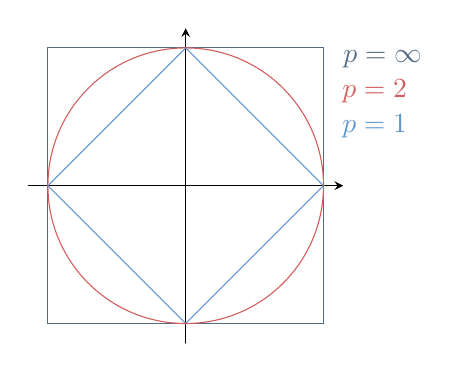
\begin{tikzpicture}[
      >=stealth,scale=1,line cap=round,
      bullet/.style={circle,inner sep=0.5pt,fill}
   ]
      \draw[->] (-2,0) -- (2,0);
      \draw[->] (0,-2) -- (0, 2);

      \draw[DarkBlue1] (-1.75,0)--(-1.75,1.75)--(0,1.75)--(1.75,1.75)--(1.75,0)--(1.75,-1.75)--(0,-1.75)--(-1.75,-1.75)--cycle;
      \draw[BrightBlue1] (-1.75,0)--(0,1.75)--(1.75,0)--(0,-1.75)--cycle;
      \draw[BrightRed1](0,0) circle (1.75);

      \draw[DarkBlue1] node at (2.5, 1.60) {$p = \infty$};
      \draw[BrightRed1] node at (2.4, 1.20) {$p = 2$};
      \draw[BrightBlue1] node at (2.4, 0.75) {$p = 1$};
   \end{tikzpicture}   
\end{center}

\pagebreak
\subsection*{\subsecstyle{Exemples de boules en dimension infinie {:}}}
On considère ici l'espace vectoriel des \textbf{fonction continues} sur l'intervalle \(\icc{a}{b}\), on peut alors étendre les \textbf{normes de Hölder} définies comme suit:
\[ 
   {||f||}_p = \left (\int_{a}^{b} |f(t)|^p dt \right)^{\frac{1}{p}}
\]

En particulier pour \(p=2\), c'est \textbf{la norme euclidienne standard}. On peut aussi définir \textbf{la norme infini} (aussi appelée \textbf{norme de la convergence uniforme}) par:
\[ 
   {||f||}_\infty = \underset{t\in \icc{a}{b}}{\sup}\{|f(t)|\}
\]

Graphiquement, la boule ouverte de centre la fonction \(\sin\) et de rayon \(1\) pour la norme infini est alors:\<

\begin{center}
   \begin{tikzpicture}[
      >=stealth,scale=1,line cap=round,
      bullet/.style={circle,inner sep=0.5pt,fill}
   ]
      \draw[->] (0,-2) -- (0, 3);
      \draw[] (-0.1,0) -- (0.1, 0) node at (-0.3, 0) {$0$};
      \draw[] (-0.1,1) -- (0.1, 1) node at (-0.3, 1) {$1$};
      \draw[] (-0.1,2) -- (0.1, 2) node at (-0.3, 2) {$2$};
      \draw[] (-0.1,-2) -- (0.1, -2) node at (-0.45, -2) {$-2$};
      \draw[] (-0.1,-1) -- (0.1, -1) node at (-0.45, -1) {$-1$};

      \draw[color=BrightRed1, domain=0:12, smooth]   plot (\x,{sin(\x r)}) node[right] {$\sin(t)$}; 
      \draw[color=BrightRed1!60,name path=A, domain=0:12, smooth, dashed]   plot (\x,{sin(\x r) + 1}); 
      \draw[color=BrightRed1!60,name path=B, domain=0:12, smooth, dashed]   plot (\x,{sin(\x r) - 1}); 
   \end{tikzpicture}   
\end{center}
\subsection*{\subsecstyle{Exemples de boules exotiques {:}}}
Si on considère maintenant l'ensemble des cases d'un échiquier et qu'on définit la distance entre deux cases comme étant le nombre de coup qu'un cavalier doit effectuer pour arriver à la seconde en partant de la première, on définit alors un espace métrique.

\chapter*{\chapterstyle{V --- Limite et continuité}}
\addcontentsline{toc}{section}{Limite et continuité}
L'intérêt fondamental de la topologie est de pouvoir définir le concept de \textit{proximité} entre points d'un espace topologie, et par la suite de définir le concept fondamental en analyse, celui de \textbf{limite} d'une suite ou d'une fonction, puis par la suite celui de \textbf{continuité} d'une fonction.\<

Une des idées principales à retenir de ce chapitre est que la notion de limite est \textbf{locale} au sens où elle nécessite que des propriétés soient vérifiées au voisinage de certains point. A contrario la notion de \textbf{continuité} est ambivalente, on peut à la fois la définir localement (propriété au voisinage d'un point) ou globalement (propriété sur les topologies des deux espaces).\<

Dans toute la suite, on considèrera que tout les espaces topologiques considérés sont \textbf{séparés}, ce qui nous permettra alors d'avoir unicité de la limite.

\subsection*{\subsecstyle{Limite d'une fonction{:}}}
On se donne une application \(f : (X, \mathcal{T}) \longmapsto (Y, \mathcal{T}')\), et on considère un point \(a\) \textbf{adhérent} à \(X\). On dira alors que la fonction \(f\) tends vers \(l \in Y\) en \(a\) si et seulement si:
\[
   \forall \; V_l \in \mathscr{V}_l \; , \; \exists  V_a \in \mathscr{V}_a \; ; \; f(X \cap V_a) \subset V_l 
\]
On notera alors \(\lim_{x \rightarrow a} f(x) = l\). Il est à noter que l'on a ici pris le parti-pris de définir la notion de limite via les voisinages, on aurait aussi pu la définir directement via les ouverts, il suffit de remplacer "voisinage de \(x\)" par "ouvert qui contient \(x\)".
\subsection*{\subsecstyle{Limite d'une suite{:}}}
Le cas d'une suite \(u : \N \longrightarrow X\) est similaire, en effet on veut alors une limite quand l'indice de la suite tends vers l'infini, on définit alors un voisinage de l'infini comme une partie qui continent un intervalle entier ouvert et infini à droite, et on obtient la définition suivante:
\[
   \forall \; V_l \in \mathscr{V}_l \; , \; \exists  V_\infty \in \mathscr{V}_\infty \; ; \; u({V_\infty}) \subset V_l 
\]
Néanmoins dans le cas des suites, la notion de limite est souvent trop contraignante et on peut vouloir s'intéresser aux valeurs qui sont prises \textbf{un infinité de fois} par la suite, on les appelera alors \textbf{valeurs d'adhérence} qu'on définit par:
\[
   \text{vadh}(u_n) := \{ x \in X \; ; \; \forall V_x \in \mathcal{V}_x , u_n \subseteq V_x \text{ pour une infinité d'indices} \}
\]
\subsection*{\subsecstyle{Continuité locale{:}}}
On peut définir une notion de continuité \textbf{locale} d'une fonction \(f: X \longrightarrow Y\) en un point \(a\) de son domaine de définition cette fois, qui ne nécessite donc que de vérifier des propriétés au voisinage d'un point, en effet on dira que \(f\) est \textbf{continue} en \(a\) si et seulement si on a:
\[
   \lim_{x \rightarrow a} f(x) = f(a)
\] 
On remarque alors la nuance entre la notion de limite et celle de continuité:
\begin{center}
   \textit{La limite est définie sur un point de l'adhérence du domaine de définition tandis que la continuité l'est sur un point du domaine de définition.}
\end{center}
En outre, on peut alors définir le \textbf{prolongement par continuité} d'une fonction \(f\) qui admet une limite \(l\) en \(a \in \text{adh}(X)\) par:
\[
   \begin{aligned}
      \widetilde{f}: X \cup \{a\} &\longrightarrow Y \\
      x &\longmapsto \begin{cases}
         f(x) \; ; \; x \in X\\
         \lim_{a} f(x) \; ; \; x = a
      \end{cases} 
   \end{aligned}
\]
\subsection*{\subsecstyle{Continuité globale{:}}}
On peut alors définir une notion de continuité \textbf{globale}, qui ne dépend que des topologies au départ et à l'arrivée, et on dira alors que \(f: X \longrightarrow Y\) est \textbf{continue} si et seulement si pour tout ouvert \(\mathcal{O} \in \mathcal{T}_Y\), on a:
\[
   f^{-1}(\mathcal{O}) \in \mathcal{T}_X  
\]
\begin{center}
   \textit{Une application est continue si la préimage de tout ouvert de l'arrivée est un ouvert du départ.}
\end{center}
On a peut alors relier les deux notions de continuité par la propriété suivante:
\begin{center}
   \textbf{Une application est (globalement) continue ssi elle est (localement) continue en tout ses points.}
\end{center}
Il est important de noter alors que si \(f\) est continue, cela \textbf{ne dit rien} de l'image direct d'un ouvert ou d'un fermé. On appelle application ouverte (resp. fermée) une application telle que l'image d'un ouvert (resp. fermé) est ouvert (resp. fermé).
\subsection*{\subsecstyle{Caractérisations métriques{:}}}
Dans le cas particulier des espaces métriques, on peut caractériser la définition de la limite de \(f\) en un point \(a\) par la métrique et les boules, et on a alors que \(\lim_{x \rightarrow a} f(x) = l\) si et seulement si:
\[
   \forall \epsilon > 0 , \exists \delta > 0 , \forall x \in X \; ; \; d(x, a) < \delta \implies d(f(x), l) < \epsilon
\]
Moralement on l'interprète par:
\begin{center}
   \textit{Il existe un \(\delta\) tel que si \(x\) est \(\delta\)-proche de \(a\) alors \(f(x)\) est arbitrairement proche de la limite.}
\end{center}
Dans le cas des suites c'est légérement différent, le voisinage de l'infini devient simplement un entier à partir duquel la propriété est vérifiée et on a que \(u_n \longrightarrow l\) si et seulement si:
\[
   \forall \epsilon > 0 , \exists N \in \N , \forall n \in \N \; ; \; n > N  \implies d(u_n, l) < \epsilon
\]
Enfin, on peut grandement simplifier la définition d'un valeur d'adhérence dans le cas métrique, en effet on obtient alors que \(l\) est une valeur d'adhérence si et seulement si:
\[
   \forall \epsilon > 0 , \forall N \in \N , \exists n \in \N \; ; \; n > N \implies d(u_n, l) < \epsilon
\]
Qui représente bien l'idée que la suite \(u_n\) de rapproche de \(l\) une infinité de fois.
\subsection*{\subsecstyle{Caractérisations séquentielles{:}}}
Dans le cadre des espaces \textbf{métriques}, on peut caractériser l'adhérence d'une partie par les suites:
\begin{center}
   L'adhérence de \(A\) est exactement \textbf{l'ensembles des limites des suites} à valeurs dans \(A\).
\end{center}
On a aussi la caractérisation séquentielle de la limite et on dira que \(\lim_{x \rightarrow a} f(x) = l\) si et seulement si pour toute suite\footnote[1]{En particulier si on trouve deux suites \(u_n, v_n\) qui tendent vers \(a\) telles que \(f(u_n), f(v_n)\) ont deux limites différentes, alors la limite de \(f\) en \(a\) ne peut pas exister.} \(u_n\) qui tends vers \(a\) on a:
\[
   \lim_{n \rightarrow +\infty} f(u_n) = l
\]
Et on peut alors aussi en déduire une caractérisation séquentielle de la continuité qui sous les mêmes hypothèses nous donne que:
\[
   \lim_{n \rightarrow +\infty} f(u_n) = f(\lim_{n \rightarrow +\infty}u_n) = f(a)
\]
\pagebreak

\subsection*{\subsecstyle{Homéomorphismes{:}}}
On considère deux espaces topologiques \(E\) et \(F\), ainsi qu'une fonction \(f : E \longrightarrow F\), alors on dit que \(f\) est \textbf{un homéomorphisme} si et seulement si elle est \textbf{bijective, continue et à réciproque continue}, on dira alors que \(E\) et \(F\) sont \textbf{homéomorphes}.\<

Les homéomorphismes sont les isomorphismes pour la structure d'espace topologique, on peut alors en déduire que toutes les propriétés intrinséquement topologiques sont conservées. Quelles sont alors les propriétés intrinséquement topologiques ? On peut alors montrer que les propriétés suivantes sont des propriétés topologiques:
\begin{itemize}
   \item La connexité.
   \item La connexité par arcs.
   \item La compacité.
\end{itemize}
Ces concepts fondamentaux en topologie sont définis dans les chapitres suivants.

\subsection*{\subsecstyle{Continuité uniforme {:}}}
\addcontentsline{toc}{subsection}{Continuité uniforme}
Dans les espaces métriques, il existe une propriété de régularité \textbf{plus forte que la continuité} appelée \textbf{continuité uniforme}\footnote[1]{Il est important de noter que la continuité uniforme n'est plus une propriété locale, mais globale.} définie comme:
\[
   \forall \epsilon > 0 , \exists \delta > 0 , \forall (x_1, x_2) \in E^2 \; ; \; d(x_1 - x_2) < \delta \implies d(f(x_1) - f(x_2)) < \epsilon 
\]

La différence fondamentale\footnote[2]{Ecrire la proposition "\(f\) est continue en tout point de \(\ioo{a}{b}\)" et "\(f\) est uniformément continue sur \(\ioo{a}{b}\)" pour le voir.} entre ces deux propriétés étant que \(\delta\) \textbf{ne dépend plus que de \(\epsilon\)}. En particulier on peut l'interpréter:
\begin{center}      
   \textit{Il existe un \(\delta\) tel que si \(x\) et \(y\) sont \(\delta\)-proches alors \(f(x)\) et \(f(y)\) soient arbitrairement proches.}
\end{center}
\subsection*{\subsecstyle{Lipschitzianité{:}}}
\addcontentsline{toc}{subsection}{Lipschitzianité}
Dans les espaces métriques, il existe une condition de régularité \textbf{encore plus forte} que la continuité uniforme qui est le caractère \(K\)-lipschitzien. On dit qu'une fonction est \(K\)-lipschitzienne pour \(K \in \R\) si et seulement si pour tout \(x, y\) distincts, on a:
\customBox{width=5cm}{
   \(d(f(x) - f(y)) \leq Kd(x - y)\)
}
\begin{center}
   \textit{
      Une telle fonction a donc la particularité de ne pas pouvoir croitre ou décroitre trop rapidement.
   }
\end{center}
La \(K\)-lipschitziannité étant une propriété plus forte que la continuité uniforme, plus précisément, on a la suite d'implications:
\[
   K\text{-Lipschitzienne} \implies \text{Uniformément continue} \implies \text{Continue}
\]


Par ailleurs si \(K \in \ico{0}{1}\), alors on dit que \(f\) est \textbf{contractante}, ce type de fonctions a souvent un trés bon comportement de convergence quand on le retrouve comme propriété de suites récurrentes par exemple.

\chapter*{\chapterstyle{V --- Connexité}}
\addcontentsline{toc}{section}{Connexité}
On considère un espace topologique \((E, \mathcal{T})\), on dira alors qu'un tel espace est \textbf{connexe} si et seulement si il ne peut \textbf{pas} s'écrire comme la réunion de \textbf{deux ouverts disjoints et non-vides}. Cela reflète alors la compréhénsion naturelle qu'on a du concept de connexité, ie que l'espace est "d'un seul tenant".\<

On peut alors définir la connexité d'une partie \( A \subseteq E \) par sa connexité en tant qu'espace muni de la topologie induite.
\subsection*{\subsecstyle{Caractérisations{:}}}
On peut alors montrer plusieurs caractérisations de la notion de connexité et on dira qu'un espace \( E \) est connexe ssi il vérifie une des conditions équivalentes suivantes:
\begin{itemize}
   \item Le seul \textbf{ouvert-fermé} non-vide de \( E \) est lui-même.
   \item Toute fonction continue \( f : E \longmapsto \left\{ 0, 1 \right\}  \) est \textbf{constante}.
\end{itemize}
La première caractérisation s'obtient directement par équivalences avec la définition, et la seconde démontre le fait qu'une fonction continue dans un espace discret est moralement une indicatrice des composantes connexes.
\subsection*{\subsecstyle{Connexité par arcs{:}}}
On peut alors définir une notion de connexité plus forte, qui utilise la notion de \textbf{chemin} que nous allons définir. On fixe deux points \(x, y \in E\), alors un chemin reliant \(x\) et \(y\) est une application \(\gamma: \icc{0}{1} \longrightarrow E\) qui est \textbf{continue} et qui vérifie:
\[
   \begin{cases}
      \gamma(0) = x \\
      \gamma(1) = y
   \end{cases}
\]
On peut alors définir la notion de connexité par arcs, en effet on dira qu'un espace est \textbf{connexe par arcs} si et seulement si \textbf{toute paire de points de \(E\) peut être réliée par un chemin.}\<

C'est une notion strictement plus forte que la connexité, en effet on peut montrer l'implication suivante:
\begin{center}
   \(E\) connexe par arcs \(\implies\) \(E\) connexe
\end{center}

\subsection*{\subsecstyle{Propriétés{:}}}
On peut alors montrer les propriétés suivantes:
\begin{itemize}
   \item L'union de parties connexes (resp. connexes par arcs) qui ont un point commun est connexe (resp. connexes par arcs).
   \item Le produit d'espaces connexes (resp. connexes par arcs) est connexe (resp. connexes par arcs).
   \item Tout partie \( B \) encadrée par un connexe \( A \) et son adhérence est connexe, ie si \( B \) est telle que:
   \[ 
      A \subseteq B \subseteq \text{adh}(A) 
   \]
   Alors \( B \) est connexe, en particulier l'adhérence d'un connexe est connexe.
\end{itemize}
\subsection*{\subsecstyle{Composantes connexes{:}}}
Si on considère un espace topologique \(E\) et un point \(x \in E\), alors toutes l'union des parties connexes qui contiennent \(x\) est connexe et c'est la plus grande partie connexe qui contient \(x\) pour l'ordre de l'inclusion, on l'appelle alors \textbf{composante connexe} de \(x\) dans \(E\) et on la note \(C_x\).\<

On peut alors partitionner l'espace en les composantes connexes de ses points, en particulier si l'espace est lui-meme connexe, il n'y a qu'une seule composante connexe. On peut de manière équivalente définir les \textbf{composantes connexes par arcs}.

\subsection*{\subsecstyle{Théorème des valeurs intermédiaires{:}}}
Les espaces connexes ont beaucoup de bonnes propriétés analytiques, tout d'abord on a la propriété suivante:
\begin{center}
   \textbf{L'image d'un connexe par une application continue est un connexe.}
\end{center}
On peut alors commencer à distinguer l'intéret de la notion de connexité, en effet on peut alors généraliser le théorème des valeurs intermidéaires à des fonctions définies sur une partie de \(\R^n\) et on a:
\begin{center}
   \textbf{L'image par une fonction continue à valeurs rélles définie sur un connexe est un intervalle.}
\end{center}

\subsection*{\subsecstyle{Passage du local au global{:}}}
Une des forces de la notion de connexité est qu'elle permet de \textbf{passer du local au global}, ie de considèrer une propriété vraie localement et de l'étendre à une propriété globale, par exemple on peut montrer la propriété suivante:
\begin{center}
   Si \( E \) est connexe et que la fonction \( f : E \longmapsto \R^n \) est \textbf{localement constante}, alors elle est \textbf{constante}.
\end{center}
\subsection*{\subsecstyle{Inversion des quantificateurs{:}}}
Une autre interprétation de la notion de connexité est qu'elle permet \textbf{d'inverser les quantificateurs d'une propriété}, par exemple supposons qu'une fonction \( f : E \longmapsto D \) soit continue et que \( D \) soit un espace discret, alors:
\[ 
   \forall t \in E \; ; \; \exists n \in D \; ; \; f(t) = n 
\]
Equivaut à:
\[ 
   \forall t \in E \; ; \; f(t) \in D
\]
Mais \( D \) est discret donc ses connexes sont les singletons et on a que \( f(E) \) est connexe donc elle est constante, ie:
\[ 
   \exists n \in D \; ; \; \forall t \in E \; ; \; f(t) = n
\]
Ce qui nous a bien permi d'inverser les quantificateurs.

\chapter*{\chapterstyle{V --- Compacité}}
\addcontentsline{toc}{section}{Compacité}
On considère un espace topologique \((E, \mathcal{T})\) et un \textbf{recouvrement ouvert} de cet espace, ie une famille quelconque \((A_i)_{i \in I}\) d'ouverts de \(E\) telle que:
\[
   E \subseteq \bigcup_{i \in I} A_i  
\]
On dira alors que l'espace est \textbf{compact} si il vérifie \textbf{la propriété de Borel-Lebesgue}, ie:
\customBox{width=12cm}{
   \begin{center}
      \textbf{De tout recouvrement, on peut extraire un recouvrement fini.}
   \end{center}
}
\subsection*{\subsecstyle{Séparation et fermeture{:}}}
Dans le cas où l'espace ambiant est séparé, on a une propriété trés forte sur les compacts, en effet on peut montrer que la topologie de \( E \) sépare les compacts et les points qui n'en font pas partie et par suite que \textbf{tout compact est fermé}.\<

Par la suite on s'intéressera surtout aux espaces séparés, donc on considérera que l'espace ambiant l'est toujours.

\subsection*{\subsecstyle{Propriétés{:}}}
On peut alors montrer les propriétés suivantes:
\begin{itemize}
   \item \textbf{Union:} Toute union \textbf{finie} de compacts est compacte.
   \item \textbf{Intersection:} Toute intersection de compacts est compacte.
   \item \textbf{Produit Cartésien:} Tout produit de compacts est compact.
   \item Tout fermé inclu dans un compact est compact.
\end{itemize}
\subsection*{\subsecstyle{Théorème de Bolzano-Weierstrass{:}}}
En considérant une suite d'un espace compact \( E \), on peut alors montrer (via le théorème des compact emboités) le théorème de Bolzano-Weierstrass:
\begin{center}
   Tout suite d'une espace compact admet \textbf{une valeur d'adhérence}.
\end{center}
En particulier dans un espace métrique, les valeurs d'adhérence sont exactement les limites de sous-suites, donc tout suite dans un compact admet une \textbf{sous-suite convergente}.

\subsection*{\subsecstyle{Caractérisation séquentielle{:}}}
Dans un espace métrique, on a même la réciproque et on peut donc caractériser les parties compactes par les suites, en effet on dira que \(K \subseteq E\) est compact si et seulement si:
\begin{center}
   \textbf{Toute suite à valeurs dans \(K\) admet une suite extraite convergente.}
\end{center}
Cette caractérisation permet alors parfois de démontrer plus facilement la compacité.

\subsection*{\subsecstyle{Théorème de Borel-Lebesgue {:}}}
Dans les espaces métriques, on peut alors obtenir d'autres propriétés des parties compactes, en effet on peut montrer qu'elles sont \textbf{bornées}, notamment en montrant que leur diamètre est fini. Dans \(\R^n\) et donc dans tout espace vectoriel normé, on a même l'équivalence entre fermé-borné et compact, appelé théorème de Borel-Lebesgue:
\begin{center}
   \textbf{Une partie de \(\R^n\) est compacte si et seulement si elle est fermée est bornée.}
\end{center}

\subsection*{\subsecstyle{Théorème des bornes atteintes{:}}}
Les espaces compacts ont beaucoup de bonnes propriétés analytiques, tout d'abord on a la propriété suivante:
\begin{center}
   \textbf{L'image d'un compact par une application continue est un compact.}
\end{center}
On peut alors commencer à distinguer l'intéret de la notion de compacité, en effet l'image de compacts par des applications continues est alors toujours bornée et fermée ce qui rends l'étude d'extrema trés simple, en particulier on peut montrer la généralisation du théorème des bornes atteintes:
\begin{center}
   \textbf{Tout fonction continue à valeurs rélles définie sur un compact est bornée et atteint ses bornes.}
\end{center}
\subsection*{\subsecstyle{Théorème de Heine{:}}}
Un résultat trés utile sur la compacité est le \textbf{théorème de Heine} qui nous permet d'affirmer que les fonctions continues définies sur des compacts sont plus régulières encore:
\begin{center}
   \textbf{Tout fonction continue définie sur un compact y est uniformément continue.}
\end{center}

\chapter*{\chapterstyle{V --- Complétude}}
\addcontentsline{toc}{section}{Complétude}
On s'intéresse dans ce chapitre à une structure plus riche que celle d'espace topologique, en effet on peut remarque que la notion d'homéomorphisme ne preserve certaines notions analytiques, comme l'équivalence entre distances, ou encore le concept que l'on définira plus loin apellé \textbf{suites de Cauchy}. On considère donc une version plus restricive d'homéomorphisme, appelée \textbf{homéomorphisme uniforme}, où l'on requiert que l'homéomorphisme soit uniformément continu.\<

C'est donc bien une notion purement métrique, et elle définit les transformation qui préservent les \textbf{invariants uniformes}, comme la complétude, le caractére de Cauchy d'une suite, qui ne sont donc pas des invariants topologiques.

\subsection*{\subsecstyle{Suites de Cauchy{:}}}
On se donne une suite \(u_n\), on dira que \(u_n\) est \textbf{de Cauchy} si et seulement si:
\[
   \forall \epsilon > 0 , \exists N \in \N , \forall p, q > N \; ; \; d(u_p - u_q) < \epsilon
\] 
\begin{center}
   \textit{
       Une suite de Cauchy est donc une suite telle que les termes de la suite sont arbitrairement proches \textbf{les uns des autres} à partir d'un certain rang\footnote[1]{Un corollaire immédiat est que \textbf{toute suite convergente est de Cauchy}.}.
   }
\end{center}
On peut alors trés facilement montrer que tout suite de Cauchy est bornée, et surtout une condition suffisante trés forte de convergence, en effet:
\begin{center}
   \textbf{Toute suite de Cauchy admettant une valeur d'adhérence converge.}
\end{center}
C'est le premier exemple d'invariant uniforme, en effet si on considère \( f : E \longmapsto F \) un homéomorphisme uniforme et \( (x_n) \) une suite de Cauchy de \( E \), alors \( (f(x_n)) \) est une suite de Cauchy.

\subsection*{\subsecstyle{Complétude{:}}}
On définit alors la structure principale de ce chapitre:
\begin{center}
   \textbf{On appelle alors espace complet tout espace métrique dans lequel toute suite de Cauchy converge.}
\end{center}
En particulier, si \( E \) est un espace vectoriel normé, on dira que c'est un \textbf{espace de Banach}. On peut alors montrer que \( \R \) est complet, en effet si on considère une suite de Cauchy de \( \R \), elle est bornée et donc incluse dans un compact, et d'aprés Bolzano-Weierstrass, elle admet une valeur d'adhérence donc elle converge.\<

On peut alors en déduire un lien entre compacité et complétude, gràce à Bolzano-Weierstrass, on montre directement que \textbf{tout espace compact est complet.}

\subsection*{\subsecstyle{Complétude et fermeture {:}}}
On peut alors montrer un lien fort entre la complétude et la fermeture, en effet gràce à la caractérisation séquentielle, on peut montrer qu'une partie complète est nécessairement \textbf{fermée}. La réciproque est partiellement vraie, en effet on a:
\begin{center}
   Une partie fermée \textbf{d'un espace complet} est complète.
\end{center}
\subsection*{\subsecstyle{Produit d'espaces complets {:}}}
On peut alors montrer que pour tout famille (finie) d'espaces métriques, alors le produit cartésien est \textbf{complet} (pour la distance produit). En particulier, \( \R^n \) et \( \C^n \) sont complets, et tout espace vectoriel de dimension finie est complet.
\subsection*{\subsecstyle{Caractérisation par les séries{:}}}
On peut alors montrer une caractérisation puissante de espaces de Banach, en effet:
\begin{center}
   \textbf{Un espace vectoriel normé est complet si et seulement si toute série absolument convergente est convergente.}
\end{center}

\subsection*{\subsecstyle{Théorème du point fixe de Banach-Picard{:}}}
Une application puissante de la complétude qui est utilisée dans beaucoup d'applications numériques est le théorème du point fixe de Banach-Picard, on considère une fonction \( f : E \longmapsto E \) où \( E \) est \textbf{complet} et telle que \( f \) soit \textbf{contractante}, ie:
\[ 
   \exists K \in \ioo{0}{1} \; , \; \forall x, y \in E \; ; \; d(f(x), f(y)) \leq K d(x, y) 
\]
Alors \( f \) admet \textbf{un unique point fixe} \( x^* \). Pour \( x_0 \in E \), on peut l'obtenir comme limite de la suite récurrente suivante:
\[ 
   x_{n+1} = f(x_n)
\]
En effet, on montre que cette suite est bien de Cauchy donc converge vers un point fixe. L'unicité est obtenue aisément par l'absurde.
   \pagebreak   
   
   \addcontentsline{toc}{chapter}{Analyse Réelle} % Pas mal
   \chapter*{\chapterstyle{VI --- Corps des Réels}} % 95% Fini
\addcontentsline{toc}{section}{Corps des Réels}
On peut construire successivement les différents ensembles \(\N, \Z, \Q\) et on souhaite maintenant construire le corps bien connu \(\R\), on peut alors construire les nombres réels comme \textbf{classes d'équivalence de suite de Cauchy de rationnels}, et on peut alors montrer la propriété caractéristique de \(\R\) qui est:
\begin{center}
   \textbf{C'est l'unique corps totalement ordonné complet qui vérifie la propriété d'Archimède.}
\end{center}
\subsection*{\subsecstyle{Propriété d'Archimède {:}}}
Un corps totalement ordonné est archimédien si et seulement si:
\[
   \forall (a, b) \in \R^*_+ \; , \; \exists n \in \N \; ; \; na > b
\]
Moralement,
\begin{center}
    \textit{
        Tout nombre de \(\R\) peut être dépassé par un multiple entier d'un autre nombre de \(\R\).
    }
\end{center}
Une autre interprétation est \textbf{qu'il n'existe pas de nombre infiniment grand ou petit} dans \(\R\), pour le voir il suffit de poser \(a = 1\) ou \(b = 1\).
\subsection*{\subsecstyle{Propriété de la borne supérieure {:}}}
On appelle alors majorant (resp. minorant) d'une partie \(A\) un réel qui est plus grand (resp. plus petit) que tout élément de \(A\), on s'intéresse alors à l'existence de \textbf{plus petit majorant} (ou de plus grand minorant), qu'on appelera alors \textbf{borne supérieure} (ou inférieure) de \(A\).
On peut alors montrer que le corps des réels vérifie \textbf{la propriété de la borne supérieure}, donnée par:
\begin{center}
   \textbf{Toute partie non-vide et majorée (resp. minorée) admet une borne supérieure (resp. inférieure)}
\end{center}
On les note alors respectivement \(\sup(A)\) et \(\inf(A)\).
\subsection*{\subsecstyle{Caractérisation séquentielle {:}}}
On peut montrer que \(M\) est la borne supérieure de \(A \subseteq \R\) si et seulement si:  
\[
   \exists (u_n) \in A^\N \; ; \; u_n \longrightarrow M
\]
\begin{center}
    \textit{
        Un majorant \(M\) est la borne supérieure de \(A\), si et seulement si il existe une suite à valeurs dans \(A\) qui tends vers \(M\).
    }
\end{center}
\subsection*{\subsecstyle{Caractérisation métrique {:}}}
Soit \(\epsilon > 0\), alors \(M\) est la borne supérieure de \(A \subseteq \R\) si et seulement si:  
\[
   \exists a \in A \; ; \; M - \epsilon \leq a \leq M
\]

\begin{center}
    \textit{
        Un majorant \(M\) est la borne supérieure de \(A\), si tout nombre plus petit n'est plus un majorant.
    }
\end{center}
\subsection*{\subsecstyle{Propriétés du corps des réels {:}}}
On introduit l'application valeur absolue qui sera très utile par la suite pour mesurer des écarts, elle est définie comme suit:
\[
    |x| := \max(x, -x)
\]
Cette application définit une norme et elle donne alors au corps des réels une structure d'espace vectoriel normé.
\subsection*{\subsecstyle{Partie entière {:}}}
Soit \(n \in \N\), on appelle \textbf{partie entière} d'un réel \(x\), et on note \(\lfloor x \rfloor\) \textbf{l'unique} entier relatif tel que:
\[
    \lfloor x \rfloor \leq x < \lfloor x \rfloor + 1
\]
La partie entière vérifie la propriété fondamentale suivante:
\customBox{width=3.5cm}{
    \(\lfloor x + n \rfloor = \lfloor x \rfloor + n\)
}
L'existence de la partie entière est garantie par \textbf{la propriété d'Archimède}.
\subsection*{\subsecstyle{Approximation décimale {:}}}
Soit \(n \in \N\), il peut être utile d'approximer un réel à \(n\) chiffres après la virgule, ie à \(10^{-n}\) près, la partie entière nous permet alors de le faire, et on l'obtient en exécutant l'algorithme suivant:
\[
    x \longrightarrow 10^n x \longrightarrow \lfloor 10^n x \rfloor \longrightarrow \frac{\lfloor 10^n x \rfloor}{10^n}
\]
On obtient alors une approximation à \textbf{n chiffre après la virgule} de \(x\) qu'on note \(d_n(x)\) et on a:
\customBox{width=3.5cm}{
    \[d_n(x) = \frac{\lfloor 10^n x \rfloor}{10^n}\]
}
\subsection*{\subsecstyle{Compactification {:}}}
On peut alors se rendre compte qu'une propriété manquante à \(\R\) est que ce n'est pas un espace compact, en effet on peut facilement construire des suites qui tendent vers \(\pm \infty\) et qui n'ont aucune suite extraite convergente dans \(\R\), la solution revient alors à definir la compactification de \(\R\) appellée \textbf{droite réelle achevée} par:
\[
   \overline{R} := \R \cup {-\infty, +\infty}
\]
Les opérations algébriques ne s'étendent alors pas parfaitement mais les symboles "infinis" ainsi ajoutés facilitent beaucoup l'énoncé de certains théorèmes et en particulier on a alors une meilleure propriété de la borne supérieure car on a que \textbf{toute partie non-vide admet une borne supérieure et inférieure}, éventuellement infinies.
\chapter*{\chapterstyle{VI --- Limites réelles}} % 95% Fini
\addcontentsline{toc}{section}{Limites réelles}
On sait déja étudier la convergence de fonctions et de suites depuis le chapitre sur la topologie et la définition du concept de limite, ici on étudiera plus précisément les application (et suites) dans \(\R\) ou \(\C\) et les conséquences des propriétés spécifiques de \(\R\) sur la convergence.\<

En effet la grande spécificité de \(\R\) est de pouvoir parler de fonctions \textbf{monotones} (croissantes ou décroissantes) et de fonctions \textbf{majorées ou minorées}.

\subsection*{\subsecstyle{Opérations générales sur les limites {:}}}
On considère que \(f\) et \(g\) deux applications qui admettent des limites \(l, l' \in K^*\) en \(a\).\+
Alors le passage à la limite est une opération \textbf{linéaire et multiplicative}, ie elle se comporte conformément à l'intuition par rapport aux opérations de \(\R\).\<

Dans le cas où les limites sont infinies ou nulles, des \textbf{formes indéterminées} peuvent apparaître et nécessitent les précautions usuelles pour conclure.
\subsection*{\subsecstyle{Limites latérales {:}}}
On peut définir un type spécifique de limite sur \(\R\) appelé \textbf{limites latérales} qui sont simplement des limites de restriction à droite ou a gauche de \(a\).\<

\uline{Exemple}: On dit que \(f\) admet une limite \textbf{par valeurs inférieures} et on note \(f(a^-) = \lim_{x \rightarrow a^-} f(x) = l\) si et seulement si:
\[
   \forall \epsilon > 0 , \exists \delta > 0 , \forall x \in X \; ; \; x - a < \delta \implies |f(x) - l| < \epsilon
\]
Et on peut alors caractériser l'existence d'une limite en un point par l'égalité des deux limites latérales en ce point.
\subsection*{\subsecstyle{Carcatére borné {:}}}
Une des principales conséquences du caractère métrique de \(\R\) sur les limites de fonctions est la suivante:
\begin{center}
   Toute fonction qui admet une limite en un point est \textbf{localement bornée} en ce point\footnote[1]{En particulier, si \(f\) est une suite, elle est \textbf{globalement bornée}.}.
\end{center}
\subsection*{\subsecstyle{Théorème de la limite monotone {:}}}
En utilisant à la fois la propriété de la borne supérieure et l'ordre total sur \(\R\), on peut alors montrer que:
\begin{itemize}
   \item  Si la fonction est \textbf{croissante et majorée} alors elle converge par valeurs inférieures vers \(f(x^-)\).
   \item  Si la fonction est \textbf{décroissante et minorée} alors elle converge par valeurs supérieures vers \(f(x^+)\).
   \item  Si la fonction est \textbf{croissante} et \textbf{non majorée} alors elle tends vers \(+ \infty\).
   \item  Si la fonction est \textbf{décroissante} et \textbf{non minorée} alors elle tends vers \(- \infty\).
\end{itemize}
En particulier si \(f\) est une \textbf{suite}, alors les deux premiers cas se simplifient en:
\begin{itemize}
   \item Si la suite \(u_n\) est \textbf{croissante et majorée} alors elle converge vers \(\sup(\{u_n\})\).
   \item Si la suite \(u_n\) est \textbf{croissante et majorée} alors elle converge vers \(\inf(\{u_n\})\)
\end{itemize}
\pagebreak
\subsection*{\subsecstyle{Théorème d'encadrement {:}}}
Aussi soit \(f, g, h\) trois fonction telles que \(f\) et \(g\) tendent vers une limite finie \(l \in \overline{\R}\) en \(a \in \overline{\R}\), alors on a aussi le \textbf{théorème d'encadrement}:
\customBox{width=10cm}{
    \(\Bigr[\forall x \in \R \; ; \; f(x) \leq g(x) \leq h(x) \Bigr] \implies g(x) \longrightarrow l\)
}
\subsection*{\subsecstyle{Suites adjacentes {:}}}
On appelle \textbf{suites adjacentes} deux suites \((u_n)\) et \((v_n)\) telles que l'une est \textbf{croissante} et l'autre \textbf{décroissante} et telles que \((u_n - v_n) \rightarrow 0\), alors on peut montrer que les deux suites convergent vers une même limite \(l \in K\) grâce aux théorèmes précédents.
\subsection*{\subsecstyle{Limite supérieure et inférieure {:}}}
On se donne une suite \((u_n)\) \textbf{bornée}, on considère les suites numériques suivantes:
\begin{align*}
   \sup_{k \geq n}\{ u_k \} = \sup\{ u_k \; ; \; k \geq n\}\\
   \inf_{k \geq n}\{ u_k \} = \inf\{ u_k \; ; \; k \geq n\}
\end{align*}
\begin{center}
    \textit{
      Ce sont simplement les bornes supérieures et inférieures des queues de la suite. 
    }
\end{center}
On peut alors remarquer que ces suites sont monotones et bornées, donc elles convergent nécessairement\footnote[1]{En effet si on prive \((u_n)\) de termes, sa borne supérieure ne peut que décroître, et \(u_n\) étant bornée, ces suite le sont aussi.} vers des limites qu'on appelle alors les \textbf{limites supérieure et inférieure} de \((u_n)\) qu'on définit formellement par:
\[
   \begin{cases}
      \lim_{n \rightarrow +\infty}\sup_{k \geq n}\{ u_k \}\\
      \lim_{n \rightarrow +\infty}\inf_{k \geq n}\{ u_k \}
   \end{cases}
\]
On calcule donc ici la plus petite borne supérieure possible, et la plus grande borne inférieure possible, on peut alors montrer que la suite \(u_n\) converse \textbf{exactement} si ces deux limites sont égales.

\subsection*{\subsecstyle{Comparaison Asymptotique {:}}}

On dit qu'une fonction \(f\) est \textbf{dominée} par la fonction \(g\) \textbf{au voisinage} de \(a \in \overline{\R}\) et on note alors \(f = O(g)\) si et seulement si il existe une fonction \textbf{bornée} \(\theta\) telle qu'on ait la propriété ci-dessous dans un voisinage de \(a\).\+
C'est une relation de \textbf{préordre} sur les fonctions, et elle est aussi \textbf{linéaire et multiplicative}.
\[
   f(x) = \theta(x)g(x)
\]

On dit qu'une fonction \(f\) est \textbf{négligeable} devant la fonction \(g\) \textbf{au voisinage} de \(a \in \overline{\R}\) et on note alors \(f = o(g)\) si et seulement si il existe une fonction \(\epsilon\) qui tends vers 0 en \(a\) telle qu'on ait la propriété ci-dessous dans un voisinage de \(a\).\+
C'est une relation \textbf{transitive, linéaire et multiplicative}.
\[
   f(x) = \epsilon(x)g(x)
\]

On dit qu'une fonction \(f\) est \textbf{équivalente} à la fonction \(g\) \textbf{au voisinage} de \(a \in \overline{\R}\) et on note alors \(f \sim o(g)\) si et seulement si il existe une fonction \(\eta\) qui tends vers 1 en \(a\) telle qu'on ait la propriété ci-dessous dans un voisinage de \(a\).\+
C'est une \textbf{relation d'équivalence} sur les suites, et elle est aussi \textbf{multiplicative}. 
\[
   f(x) = \eta(x)g(x)
\]
Ces relations sont évidemment aussi valables pour les suites en remplaçant partout le terme "fonction" par le terme "suite".
\pagebreak

De manière générale, quand les fonctions ne s'annulent pas au voisinage de \(a\), on caractérise ces relations par le tableau suivant:
\begin{center}
   \renewcommand{\arraystretch}{1.5}%
   \setlength\arrayrulewidth{0.8pt}
   \begin{tabular}{| c | c | c |}
   \hline
   \(f = O(g) \Longleftrightarrow \frac{f}{g}(x) \longrightarrow C\) &    \(f = o(g) \Longleftrightarrow \frac{f}{g}(x) \longrightarrow 0\) &    \(f \sim g \Longleftrightarrow \frac{f}{g}(x) \longrightarrow 1\)\\ [1.5ex]
   \hline
   \end{tabular}
\end{center}  

On peut notamment caractériser le fait qu'une limite existe par:
\[
   f \longrightarrow l \Longleftrightarrow f = l + o(1)
\]   
Aussi, une caractérisation trés utile des équivalents nous donne\footnote[1]{La démonstration est triviale et utilise simplement la caractérisation en terme de quotient}:
\[
   f \sim g \Longleftrightarrow f = g + o(g)
\]

Enfin, il est utile de connaître ces équivalents usuels, on considère le cas général d'une fonction \(u\) qui tends vers 0 en \(a\), alors on a les équivalents suivants (en \(a\)):

\begin{center}
   \renewcommand{\arraystretch}{1.5}%
   \setlength\arrayrulewidth{0.8pt}

   \begin{tabular}{| c | c | c |}
   \hline
   \(ln(1 + u) \sim u\) & \(e^u - 1 \sim u\) & \((1 + u)^\alpha - 1 \sim \alpha u\)\\ [0.5ex]
   \hline
   \(\sin(u) \sim u\) & \(\cos(u) \sim 1\) & \(\tan(u) \sim u\)\\ [0.5ex]
   \hline
   \end{tabular}
\end{center} 
\begin{center}
   \textit{
      On remarquera dans le chapitre sur les développements limités que la grande majorité de ces équivalents ne sont que le premier terme non-nul du développement limité d'une fonction.
   }
\end{center}
\chapter*{\chapterstyle{VI --- Continuité}} % 99% Fini
\addcontentsline{toc}{section}{Continuité}
On étudie ici les propriétés des fonctions réelles continues, dont on sait montrer la continuité depuis le chapitre de topologie, ici on s'intéteressera aux spécificités des fonctions continues réelles, notamment leurs comportement vis à vis des opérations et les différents raffinements de la notion de continuité que l'on pourrait développer.

\subsection*{\subsecstyle{Opérations générales sur les fonctions continues {:}}}
On note \(\mathscr{C}(D, \K)\) l'ensemble des fonctions continues sur \(D\) à valeurs dans \(\K\), alors on peut montrer que cet ensemble est stable par somme, multiplication externe et mulplication interne.
\begin{center}
   \textit{
      En d'autres termes cet ensemble est non seulement un \textbf{sous-espace vectoriel} de l'espace des fonctions, mais même une \textbf{sous-algèbre} de cet espace.
   }
\end{center}
De plus, l'inverse d'une fonction continue qui ne s'annule pas est aussi une fonction continue, et la composition de fonctions continues composables est aussi une fonction continue\footnote[1]{Attention pour la composition il faut bien considèrer les domaines de défintion manipulés.}.
\subsection*{\subsecstyle{Prolongement par continuité {:}}}
\addcontentsline{toc}{subsection}{Prolongement par continuité}

Considérons une fonction \(f\) continue sur un intervalle \(I \backslash \{a\}\), telle que sa limite en \(a\) existe, alors on peut considèrer la fonction \(\widetilde{f}\) définie par:
\[
   \begin{aligned}
      \widetilde{f}: I &\longrightarrow \R \; ; \; x &\longmapsto \begin{cases}
         \widetilde{f}(a) = \lim_{a} f(x) \text{ si } x = a\\
         \widetilde{f}(x) = f(x) \text{ sinon}
      \end{cases}
   \end{aligned}
\]
Alors par construction \(\widetilde{f}\) est bien continue sur tout \(I\) et on l'appelle \textbf{le prolongement par continuité} de \(f\) en \(a\).
\subsection*{\subsecstyle{Théorème des valeurs intermédiaires{:}}}
\addcontentsline{toc}{subsection}{Théorème des valeurs intermédiaires}
Le chapitre de topologie nous a permi de montrer que l'image d'un connexe par une application continue est un connexe, or dans les réels, on a que:
\begin{center}
   \textbf{Les connexes de \(\R\) sont exactements les intervalles.}
\end{center}
On en déduit donc le théorème des valeurs intermédiaires:
\begin{center}
   \textbf{L'image continue d'un intervalle est un intervalle.}
\end{center}
\subsection*{\subsecstyle{Théorème des bornes atteintes{:}}}
Le chapitre de topologie nous a aussi permi de montrer que l'image d'un compact par une application continue est un compact, or dans les réels, on a donc dans ce cas particulier deux conséquences:
\begin{itemize}
   \item L'image continue d'un compact est borné.
   \item Les bornes sont atteintes.
\end{itemize}
En particulier, l'image continue d'un segment est un segment.
\subsection*{\subsecstyle{Théorème de la bijection{:}}}
On déduis du théorème des valeurs intermédiaires que si \(f\) est continue sur \(\ioo{a}{b}\) et \textbf{strictement monotone} alors:
\begin{center}
   Elle réalise \textbf{un homéomorphisme} sur son image.
\end{center}
\chapter*{\chapterstyle{VI --- Dérivabilité}} % 99% Fini
\addcontentsline{toc}{section}{Dérivabilité}

\subsection*{\subsecstyle{Définition {:}}}
\addcontentsline{toc}{subsection}{Définition}

On dit qu'une fonction \(f\) est dérivable en un point \(a\) si et seulement si la limite ci-dessous existe et est \textbf{finie} et on définit alors le nombre dérivé \(f'(a)\):
\customBox{width=4.5cm}{
   \[f'(a) := \underset{x \rightarrow a}{\lim} \frac{f(x) - f(a)}{x - a}\]
}
On peut alors définir la dérivée de la fonction \(f\) qu'on note \(f'\)  qui est la fonction qui à chaque point où \(f\) est dérivable lui associe son nombre dérivé, ainsi que \textbf{la tangente à la courbe} de \(f\) en \(a\) comme étant la droite:
\customBox{width=5cm}{
   \(y := f(a) + f'(a)(x - a)\)
}

A nouveau, le lien clair entre le concept de limite et celui de dérivabilité nous permet de définir \textbf{la dérivabilité latérale} d'une fonction, qui est simplement la dérivabilité à droite ou à gauche qui découle directement de notre définition des limites latérales d'une fonction.\<

On peut étendre cette définition à la dérivabilité sur \textbf{un intervalle} \(I\), en la définissant comme la dérivabilité en \textbf{tout points de \(I\)}.\+
On note \(\mathscr{D}(D, \K)\) l'ensemble des fonctions dérivables sur \(D\) à valeurs dans \(\K\), par ailleurs il est important de noter que \textbf{la dérivabilité implique la continuité}, ie formellement on a \(\mathscr{D}(D, \K) \subset \mathscr{C}(D, \K)\).

\subsection*{\subsecstyle{Propriétés {:}}}
\addcontentsline{toc}{subsection}{Propriétés}

Une des propriétés fondamentales des fonctions dérivables et de l'ensemble \(\mathscr{D}(D, \K)\) est qu'il est stable par somme, multiplication externe et mulplication interne.
\begin{center}
   \textit{
      En d'autres termes cet ensemble est non seulement un \textbf{sous-espace vectoriel} de l'espace des fonctions (continues), mais même une \textbf{sous-algèbre} de cet espace.
   }
\end{center}
De plus, l'inverse d'une fonction dérivable qui ne s'annule pas est aussi une fonction dérivable, et la composition de fonctions dérivables composables est aussi une fonction dérivable.

\subsection*{\subsecstyle{Etudes des variations {:}}}
\addcontentsline{toc}{subsection}{Etudes des variations}

Si on considère une fonction dérivable, alors on appelle \textbf{point critique} tout point \(a\) où \(f'(a) = 0\).\+
En particulier, si une fonction est dérivable en un point \textbf{intérieur}\footnote[1]{Si le point n'est pas intérieur et est un extremum, la dérivée n'est pas nécessairement nulle. Par exemple la restriction (à l'arrivée) de ln(x) à \(\R^-\) est dérivable à gauche en 1, y admet un maximum, mais la dérivée n'est pas nulle.} et y admet un \textbf{extremum local}, alors c'est un point critique.\<

Enfin le signe de la dérivée nous permet de comprendre les variations de la fonction sur un \textbf{intervalle}, en particulier on a la propriété suivante:
\begin{center}
   \textit{Si \(f'\) conserve le même signe sur un intervalle, alors \(f\) est monotone sur cet intervalle\footnote[2]{En particulier elle est croissante dans le cas positif et décroissante sinon}.}
\end{center}
En particulier, si \(f'\) est nulle sur un intervalle, alors \(f\) est constante sur cet intervalle.
\pagebreak 

\subsection*{\subsecstyle{Classes de régularité {:}}}
\addcontentsline{toc}{subsection}{Classes de régularité}

Les classes de régularité des fonctions numériques constituent une classification des fonctions basées sur l'existence et la continuité des dérivées itérées.
Par exemple on note \(\mathscr{C}^0(D, \K)\) l'ensemble des fonctions continues, \(\mathscr{C}^1(D, \K)\) l'ensemble des fonctions dérivables à dérivée continue.\<

En généralisant ces notations, on note \(\mathscr{C}^k(D, \K)\) l'ensemble des fonctions \(k\) fois dérivables \textbf{et à dérivée continue}.\<

Ces ensembles \textbf{héritent des propriétés de stabilité} (par somme, produit interne et externe, composition et inverses) des ensembles de base définis précédemment. En particulier ce sont tous des sous-algèbres de l'espace des fonctions.

\subsection*{\subsecstyle{Dérivation {:}}}
\addcontentsline{toc}{subsection}{Dérivation}

Soit \(f\) une fonction dérivable, alors on peut appliquer à \(f\) l'opérateur de dérivation, en d'autres termes calculer sa dérivée \(f'\). Dans cette partie nous allons détailler les propriétés élémentaires de cet opérateur:
\begin{center}
   \renewcommand{\arraystretch}{1.5}%
   \setlength\arrayrulewidth{0.8pt}

   \begin{tabular}{| c | c | c |}
   \hline
   \((f + g)' = f' + g'\) & \((fg)' = f'g + fg'\)  & \((f \circ g)' = (f' \circ g) \cdot g'\) \\ [1ex]
   \hline
   \end{tabular}
\end{center}  
Soit \(f\) de classe \(\mathscr{C}^n\), alors dans le cas de dérivées successives, la propriété pour la somme ci dessus se généralise aisément et la formule du produit, appellée \textbf{formule de Liebniz} se généralise aussi en:
\customBox{width=5.5cm}{
   \[(fg)^{(n)} = \sum_{k=0}^{n}\binom{k}{n}f^{(k)}g^{(n - k)}\]
}
Par ailleurs, si on pose \(f\) une fonction dérivable sur \(I\) et que \(f'\) ne s'annule pas sur \(I\), alors la réciproque de \(f\) est dérivable\footnote[1]{Les deux hypothèses impliquent que \(f\) est bijective sur son image, puis on revient à la définition pour montrer que \(f^{-1}\) est dérivable en \(f(a)\), on peut effectuer un changement de variable dans le calcul de limite pour trouver la première identité. La seconde nécessite un second changement de variable évident.} pour tout \(y := f(a)\) sur cet intervalle et on a:
\customBox{width=6cm}{
   \[(f^{-1})'(y) = \frac{1}{f'(a)} = \frac{1}{f'(f^{-1}(y))}\]
}
On peut généraliser ce résultat\footnote[2]{Même début de preuve que ci-dessus, avec une récurrence pour conclure.} en montrant que si \(f\) est une fonction de classe \(\mathscr{C}^k\) et si \(f'\) \textbf{ne s'annule pas}, alors \(f^{-1}\) est aussi de classe \(\mathscr{C}^k\).\<

Cette propriété permet de prouver la dérivabilité d'une réciproque, ainsi que de trouver sa dérivée.\+
\underline{Exemple:} \(f: x \mapsto x^2\) est dérivable et sa dérivée ne s'annule pas sur cet \(\icc{1}{2}\), donc elle est bijective sur \(\icc{1}{4}\) et sa réciproque est dérivable de dérivée \(\frac{1}{2\sqrt{x}}\).

\subsection*{\subsecstyle{Théorème des accroissements finis {:}}}
\addcontentsline{toc}{subsection}{Théorème des accroissements finis}

Soit \(f\) une fonction continue sur un intervalle \(\icc{a}{b}\) et dérivable sur \(\ioo{a}{b}\), le \textbf{théorème des accroissements finis} assure l'existence d'un \(c \in \ioo{a}{b}\) tel que:
\customBox{width=4.5cm}{
   \[\frac{f(b) - f(a)}{b - a} = f'(c)\]
}
Intuitivement, on comprends alors que la quantité à droite est le taux d'acroissement global entre \(a\) et \(b\), et donc le théorème nous assure l'existence d'un point tel que \textbf{le taux d'acroissement en ce point soit égal au taux d'acroissement global}.
\pagebreak

Graphiquement, on voit sur le dessin ci-dessous que les deux taux d'accroissement sont égaux:
\begin{center}
   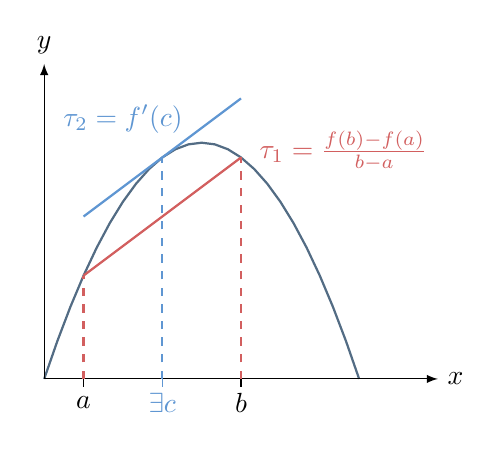
\begin{tikzpicture}[domain=0:4]
      \draw[color=DarkBlue1, thick] plot (\x,{3*\x - 0.75*\x^2});

      \draw[-latex] (0,0) -- (5,0) node [right] {$x$};
      \draw[-latex] (0, 0) -- (0,4) node [above] {$y$};


      \draw[] (0.5, -0.1) -- (0.5,0.1) node[] at (0.5, -0.3) {$a$};
      \draw[color=BrightRed1, thick, dashed] (0.5,0) -- (0.5, 1.3125);
      \draw[] (2.5, -0.1) -- (2.5,0.1) node[] at (2.5, -0.3) {$b$};
      \draw[color=BrightRed1, thick, dashed] (2.5,0) -- (2.5, 2.8125);

      \draw[color=BrightRed1, thick] (0.5, 1.3125) -- (2.5, 2.8125) node at (3.8, 2.9) {$\tau_1 = \frac{f(b) - f(a)}{b - a}$};

      \draw[color=BrightBlue1] (1.5, -0.1) -- (1.5,0.1) node[] at (1.5, -0.3) {$\exists c$};
      \draw[color=BrightBlue1, thick, dashed] (1.5, 0) -- (1.5, 2.8125);
      \draw[color=BrightBlue1, thick, domain=0.5:2.5] plot (\x,{1.6875 + 0.75*\x}) node[] at (1, 3.3) {$\tau_2 = f'(c)$};

   \end{tikzpicture}
\end{center}
Un cas particulier\footnote[1]{La preuve nécessite d'ailleurs de s'y ramener, en effet on considère la fonction \(\phi : x \mapsto \frac{f(b) - f(a)}{b-a}(x -a) + f(a)\), alors \(\phi(x) = \phi(y)\) et en sachant que la fonction est bornée et atteint ses bornes, on trouve des points critiques.} remarquable de ce théorème est le \textbf{théorème de Rolle} dans le cas où \(f(a) = f(b)\), donc dans le cas où le taux d'acroissement global est nul, alors on a l'existence d'un \(c \in \ioo{a}{b}\) tel que \(f'(c) = 0\).
\subsection*{\subsecstyle{Inégalité des accroissements finis {:}}}
\addcontentsline{toc}{subsection}{Inégalité des accroissements finis}

L'inégalité des accroissements finis donne une condition suffisante de lipschitziannité, en effet si \(f'\) est bornée, alors \(f\) est \(K\)-lipschitzienne avec \(K = \sup|f'|\), ie on a:
\[
   |f(b) - f(a)| \leq K|b-a|
\]
\underline{Exemple:} \(|\sin(x)'| = |\cos(x)| \leq 1\) donc sinus est une fonction \(1\)-lipschitzienne et donc on montre par exemple que \(|\sin(x) - \sin(0)| \leq |x - 0| \Longleftrightarrow |\sin(x)| \leq |x|\)

\subsection*{\subsecstyle{Théorème de la limite de la dérivée{:}}}
\addcontentsline{toc}{subsection}{Théorème de la limite de la dérivée}

Soit \(f\) une fonction continue sur \(I\) et dérivable sur \(I \; \backslash \; \{a\}\), alors on peut montrer que si \(\underset{x \rightarrow a}{\lim} f'(x) =  l\), alors \(f\) \textbf{est dérivable} en \(a\) de dérivée \(l\).\<

En particulier pour une fonction \(f \in \mathscr{C}^1(I \; \backslash \; \{a\}, \R)\), si \({\lim}f\) et \({\lim}f'\) existent, alors le prolongement à \(I\) tout entier est de classe \(\mathscr{C}^1\).\+
En général pour une fonction \(f \in \mathscr{C}^k(I \; \backslash \; \{a\}, \R)\), si les limites de toutes les dérivées intermédiaires existent, alors le prolongement à \(I\) tout entier est de classe \(\mathscr{C}^k\).
\chapter*{\chapterstyle{VI --- Convexité}} % 99% Fini
\addcontentsline{toc}{section}{Convexité}

\subsection*{\subsecstyle{Définition {:}}}
\addcontentsline{toc}{subsection}{Définition}

On dit que \(f\) est \textbf{convexe} sur \(I\) si et seulement si \textbf{son graphe est en dessous de toutes ses cordes}, ie elle vérifie la propriété:
\customBox{width=10cm}{
   \(\forall a, b \in I \; , \; \forall \lambda \in \icc{0}{1}\; ; \; f((1-\lambda)a + \lambda b) \leq (1-\lambda)f(a) + \lambda f(b)\)
}
Une fonction qui vérifie l'inégalité inverse est dite \textbf{concave} et son graphe est situé \textbf{au dessus de toutes ses cordes}.
Graphiquement, voici un exemple de fonction convexe:
\begin{center}
   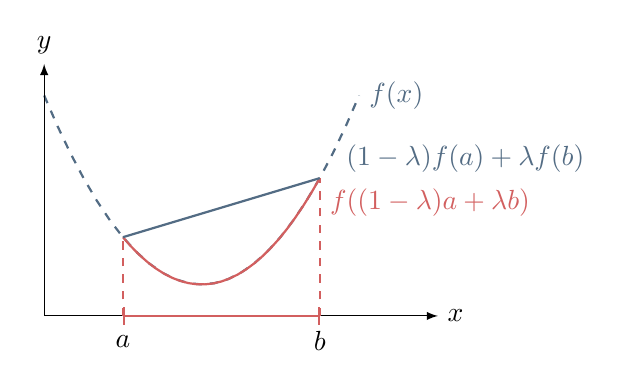
\begin{tikzpicture}[domain=0:4, yscale=0.8]
      \draw[color=DarkBlue1, thick, dashed] plot (\x,{-3*\x + 0.75*\x^2+3.5}) node [right] {$f(x)$};

      \draw[-latex] (0,0) -- (5,0) node [right] {$x$};
      \draw[-latex] (0, 0) -- (0,4) node [above] {$y$};

      \draw[|-|, thick, color=BrightRed1] (1, 0) -- (3.5,0);
      \draw node at (1, -0.4) {$a$};
      \draw node at (3.5, -0.4) {$b$};
      \draw[dashed, color=BrightRed1, thick] (1, 0) -- (1, 1.25);      
      \draw[dashed, color=BrightRed1, thick] (3.5, 0) -- (3.5, 2.1875);

      \draw[color=BrightRed1, thick, domain=1:3.5] plot (\x,{-3*\x + 0.75*\x^2+3.5}) node [below right] {$f((1-\lambda)a + \lambda b)$};

      \draw[color=DarkBlue1, thick] (1, 1.25) -- (3.5, 2.1875) node[] at (5.35, 2.5) {$(1-\lambda)f(a) + \lambda f(b)$};

   \end{tikzpicture}
\end{center}
\begin{center}
   \textit{
      En d'autres termes l'image d'un barycentre (à coefficient positif) est en dessous du barycentre des images.
   }
\end{center}
Par ailleurs il existe une caractérisation trés utile de la convexité, pour montrer qu'une fonction \textbf{dérivable} est convexe, il suffit de montrer que sa \textbf{dérivée est croissante}, ou alors, si elle est deux fois dérivable, que sa \textbf{dérivée seconde est positive}.\<

\underline{Exemple:}  La fonction logarithme est concave sur \(\R\) car sa dérivée seconde est négative, donc pour tous \(a, b > 0\), on a \(\ln(\frac{a + b}{2}) \leq \frac{1}{2}\ln(a) + \frac{1}{2}\ln(b)\).

\subsection*{\subsecstyle{Propriétés {:}}}
\addcontentsline{toc}{subsection}{Propriétés}

On peut noter deux grandes propriétés des fonctions convexes, tout d'abord pour tout \(a, b, c\) dans \(I\) tels que \(a < b < c\), on a \textbf{l'inégalité des pentes} qui nous donne:
\customBox{width=7.5cm}{
   \[\frac{f(b)-f(a)}{b-a} \leq \frac{f(c)-f(a)}{c-a} \leq \frac{f(c)-f(b)}{c-b}\]
}
Intuitivement, cela signifie que \textbf{les pentes des cordes sont croissantes}.\<

Finalement on peut généraliser l'inégalité de la définition par \textbf{l'inégalité de Jensen}, qui pour toute famille \((x_i)_{i \in \N}\) de points et famille \((\lambda_i)_{i \in \N}\) de coefficients positifs de somme 1, nous donne:
\customBox{width=5cm}{
   \[f\biggl(\sum_{i \in \N} \lambda_i x_i\biggl) \leq  \sum_{i \in \N} \lambda_i f(x_i)\]
}
Qui généralise l'intuition selon laquelle \textbf{l'image d'un barycentre est en dessous du barycentre des images}.
\chapter*{\chapterstyle{VI --- Développements limités}} % 99% Fini
\addcontentsline{toc}{section}{Développements limités}

Dans ce chapitre nous cherchons à approximer \textbf{localement} des fonctions par des polynômes au voisinage d'un point ou de l'infini.\<

Il est important de noter que la majorité des égalités de ce chapitre sont des égalités \textbf{au voisinage d'un point}, et non des égalités globales.
\subsection*{\subsecstyle{Définition {:}}}
\addcontentsline{toc}{subsection}{Définition}

Soit \(f\) une fonction de \(D\) dans \(\R\), et \(a\) un point adhérent à \(D\). On dit que \(f\) admet un \textbf{développement limité} d'ordre \(n\) \textbf{au voisinage de } \(a\) et on note \(DL_n(a)\) si il existe une famille de réels \((a_i)\) tels que:
\customBox{width=10cm}{
   \(f(x) = a_0 + a_1(x-a) + \ldots + a_n(x-a)^n + o((x-a)^n)\)
}
Si elle existe, alors cette famille est \textbf{unique}, par ailleurs plus l'ordre est grand, plus la précision est grande.\+

La partie polynomiale d'une développement limité est appellée \textbf{partie principale}.

\subsection*{\subsecstyle{Propriétés{:}}}
\addcontentsline{toc}{subsection}{Propriétés}

Soit \(f\) et \(g\) deux fonctions qui admettent un développement limité à l'ordre \(n\).\+
On appelle \textbf{troncature} à l'ordre \(k\) de \(f\), la partie principale de \(f\) privée de tout les coefficients de degré supérieurs à \(k\), et suivi d'un \(o(x^k)\). Il s'agit simplement ici de réduire la précision de notre approximation, en particulier, si on a un développement limité à l'ordre \(n\) alors on a un développement limité à tout ordre inférieur à \(n\) par troncature.\<

Aussi, les développements limités se comportent de manière intuitive par rapports aux opérations algébriques:
\begin{center}
   \textit{Pour calculer un développement limité d'une somme, il suffit de faire la somme des parties principales. \+
   Pour la multiplication (la composition), il suffit de faire le produit (la composée) des parties principales.\footnote[1]{\textbf{Attention:} Cette méthode produira dans la plupart des cas des termes inutiles, il faut donc tronquer et/ou anticiper le degré du produit final, pour faciliter les calculs, voir l'exemple.} }
\end{center}

\underline{Exemple:} Cherchons un \(DL_2(e^x\cos(x))\), on a \(e^x\cos(x) = [1 + x + \frac{x^2}{2}+o(x^2)] [1 - \frac{x^2}{2} + o(x^2)]  \) = \(1 + x + o(x^2)\)

\subsection*{\subsecstyle{Changement de voisinage {:}}}
\addcontentsline{toc}{subsection}{Changement de voisinage}

On peut ramener la recherche d'un déveoppement limité en un point à un développement limité en \(0\) par une translation.\footnote[2]{En effet, un DL\((a, f(x))\) est un DL\((0, f(x + a))\) à translation près (faire un dessin). Il suffit donc de chercher un DL\((0, f(x + a))\) puis de translater à nouveau sur la fonction originelle.}\<

On peut ramener la recherche d'un déveoppement asymptotique en \(\pm \infty\), à un développement limité en \(0\) par le changement de variable
\( X = \frac{1}{x}\).\<

\underline{Exemple:} La fonction \(e^\frac{1}{x}\) est définie au voisinage de \(+ \infty\), on pose \(X = \frac{1}{x}\), alors un \(DL_2(0)\) de \(f(X)\) est \(1 + X + \frac{X^2}{2}+o(X^2) = 1 + \frac{1}{x} + \frac{1}{2x^2} + o(\frac{1}{x^2})\) aprés substitution.
\pagebreak

\subsection*{\subsecstyle{Formules de Taylor {:}}}
\addcontentsline{toc}{subsection}{Formule de Taylor-Young}
Soit \(f\) une fonction de classe \(\mathscr{C}^n\) sur un intervalle \(I\), alors on peut montrer \textbf{l'existence} d'un développement limité à l'ordre \(n\) au voisinage d'un point \(a\) de \(I\) qui est donné par:
\customBox{width=7cm}{
   \[f(x) = \sum_{k=0}^{n} \frac{f^{(k)}(a)}{k!}(x - a)^k + o((x - a)^n)\]
}
La quantité négligeable appellée \textbf{reste}, qu'on note généralement \(R_n\), peut s'expliciter dans le cas où la fonction est de classe \(\mathscr{C}^{n+1}\) et pour un certain \(c \in \icc{a}{x}\), on a:
\customBox{width=11cm}{
   \[ R_n = \frac{f^{(k+1)}(c)}{k!}(x - a)^{k+1} 
   \quad\quad\quad\quad
   R_n = \int_{a}^{x} \frac{f^{(k+1)}(t)}{k!}(x - t)^{k} d t\]
}  
Ce sont respectivement les formules de \textbf{Taylor-Lagrange}\footnote[1]{Celle ci peut se comprendre comme une généralisation du théorème des accroissements finis qui en est un cas particulier (à l'ordre 1).} et de \textbf{Taylor avec reste intégral}.\+
Expliciter le reste permet alors d'obtenir des informations sur tout l'intervalle \(\icc{a}{x}\), en effet, ce ne sont alors plus des développements asymptotiques mais bien des formules \textbf{exactes}.\<

\underline{Exemple:} Pour un certain \(c\) sur l'intervale \(\icc{0}{x}\) , on a \(\cos(x) = 1 - \frac{x^2}{2!} + \frac{x^4}{4!} + \frac{x^5}{5!}\sin(c)\), cela nous permet alors d'avoir, par exemple, la majoration \(\cos(x) \leq 1 - \frac{x^2}{2!} + \frac{x^4}{4!} + \frac{x^5}{5!}\).
\<


Aussi, \(f\) est continue en \(a\) si et seulement si elle admet un \textbf{développement limité à l'ordre 0}.\+
De même, elle est dérivable en \(a\) si et seulement si elle admet un \textbf{développement limité à l'ordre 1}.\+
Néanmoins, au dela de l'ordre \(k = 1\), admettre un développement limité à l'ordre \(k\) n'implique \textbf{pas} d'être de classe \(\mathscr{C}^k\).

\subsection*{\subsecstyle{Intégration d'un développement limité{:}}}
\addcontentsline{toc}{subsection}{Intégration d'un développement limité}

Une propriété trés particulière nous permet de trouver le développement limité d'une fonction si l'on connaît le développement limité de sa dérivée.\+ 
Soit \(f\) une fonction dérivable tel que \(f'\) admet un développement limité à l'ordre \(n\), ie:
\[
   f'(x) \underset{0}{=} \sum_{k=0}^{n} a_kx^k + o(x^k)   
\]
Alors \(f\) admet un développement limité à l'ordre \(n + 1\) obtenu \textbf{en intégrant termes à termes}, ie on a:
\[
   f(x) \underset{0}{=} f(a) + \sum_{k=0}^{n} \frac{a_k x^{k+1}}{k+1} + o(x^{k+1})   
\]
Ici la constante d'intégration est le terme d'ordre 0 du développement limité, ie \(f(a)\).
\begin{center}
   \textit{
      Un développement limité de la dérivée nous donne donc \textbf{toujours}\+
      un développement limité de la fonction.
   }
\end{center}

\subsection*{\subsecstyle{Développements limités usuels {:}}}
\addcontentsline{toc}{subsection}{Développements limmités usuels}

Il est utile de connapitre les développements limités en \(0\) des fonctions usuelles:
\begin{center}
   \renewcommand{\arraystretch}{1.5}%
   \setlength\arrayrulewidth{0.8pt}

   \begin{tabular}{| c | c |}
   \hline
   \(e^x = 1 + x + \frac{x^2}{2} + \frac{x^3}{6} + \ldots + o(x^n)\) & \(\ln(1 + x) = x - \frac{x^2}{2} + \frac{x^3}{3} - \ldots + o(x^n) \)\\[1.5ex]
   \hline
   \((1+x)^\alpha = 1 + \binom{\alpha}{1} x + \binom{\alpha}{2}\frac{x^2}{2} + \binom{\alpha}{3}\frac{x^3}{6} + \ldots + o(x^n)\) & \(\frac{1}{1-x} = 1 + x + x^2 + x^3 + \ldots + o(x^n)\) \\[1.5ex]
   \hline
   \(\cos(x) = 1 - \frac{x^2}{2} + \frac{x^4}{24} - \ldots + o(x^n)\) & \(\sin(x) = x - \frac{x^3}{6} + \frac{x^5}{120} - \ldots + o(x^n)\) \\[1.5ex]   
   \hline
   \end{tabular}
\end{center} 
\chapter*{\chapterstyle{VI --- Intégration}} % 99% Fini
\addcontentsline{toc}{section}{Intégration}

On définira dans ce chapitre l'intégration d'une fonction \textbf{bornée définie sur un segment}.\<

On appelle \textbf{subdivision} du segment \(\icc{a}{b}\) qu'on note généralement \(\sigma\) toute suite finie \((x_i)_{i \in \N}\) strictement croissante de premier terme \(x_0 = a\) et de dernier terme \(x_n = b\), on appelle \textbf{pas de la subdivision} la distance maximale entre deux éléments consécutifs de la subdivision, qu'on note généralement \(|\sigma|\).

\subsection*{\subsecstyle{Définition {:}}}
\addcontentsline{toc}{subsection}{Définition}

Soit \(f\) une fonction définie sur un segment \(\icc{a}{b}\), et \(\sigma = (x_i)_{i \in \N}\) une subdivision de ce segment, on note \(M_i := \sup\{f(x) \; ; \; x \in \icc{x_i}{x_{i+1}}\}\) le supremum de la fonction sur chaque intervalle (qui existe car on ne considère bien que les fonctions \textbf{bornées}).\<

Alors on appelle \textbf{somme de Darboux supérieure\footnote[1]{On définit de même \textbf{la somme de Darboux inférieure} associée à la subdivision qui est analogue à la différence que la hauteur des rectangle est donnée par l'infimum de la fonction sur la subdivision.} associée à la subdivision} la somme:
\[
   ^+S(f, \sigma) = \sum_{k=0}^{n} (x_{k+1} - x_k) \cdot M_k 
\] 
Cette somme correspond à \textbf{la somme de rectangles} chacun de base \(x_{k+1} - x_k\) et de hauteur le supremum de la fonction sur cette intervalle. Graphiquement, on a:
\begin{center}
   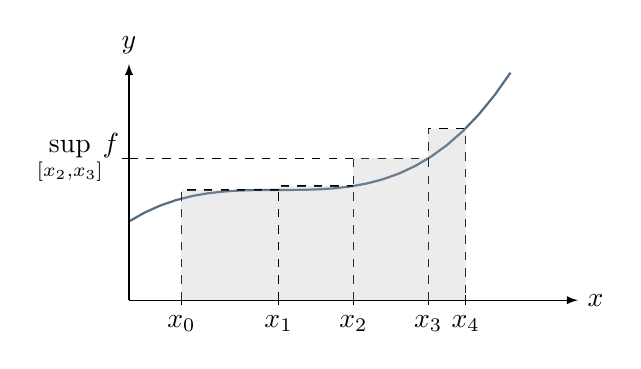
\begin{tikzpicture}[domain=0:2.55, xscale=1.9, yscale=0.6]
      \draw[color=DarkBlue1, thick] plot (\x,{((\x-1)^3 + 2)/1.5+1});
      \draw[-latex] (0,0) -- (3,0) node [right] {$x$};
      \draw[-latex] (0, 0) -- (0,5) node [above] {$y$};
      
      \draw[color = black] (0.35, 0.1) -- (0.35, -0.1) node[] at (0.35, -0.5) {$x_0$};
      \draw[dashed, color = black] (0.35, 0) -- (0.35, 2.3333) -- (1, 2.3333);
      \fill[black!30,nearly transparent] (0.35, 0) -- (0.35, 2.3333) -- (1, 2.3333) -- (1, 0) -- cycle;

      \draw[color = black] (1, 0.1) -- (1, -0.1) node[] at (1, -0.5) {$x_1$};
      \draw[dashed, color = black] (1, 0) -- (1, 2.417) -- (1.5, 2.417);
      \fill[black!30,nearly transparent] (1, 0) -- (1, 2.4166) -- (1.5, 2.4166) -- (1.5, 0) -- cycle;

      \draw[color = black] (1.5, 0.1) -- (1.5, -0.1) node[] at (1.5, -0.5) {$x_2$};
      \draw[dashed, color = black] (1.5, 0) -- (1.5, 3) -- (2, 3);

      \draw[dashed, color = black] (1.5, 3) -- (0, 3) node[color=black, left] {$\underset{\icc{x_2}{x_{3}}}{\sup}f$};
      \draw[color = black] (-0.05, 3) -- (0.05, 3);

      \fill[black!30,nearly transparent] (1.5, 0) -- (1.5, 3) -- (2, 3) -- (2, 0) -- cycle;

      \draw[color = black] (2, 0.1) -- (2, -0.1) node[] at (2, -0.5) {$x_3$};
      \draw[dashed, color = black] (2, 0) -- (2, 3.63) -- (2.25, 3.63) -- (2.25, 0);
      \fill[black!30,nearly transparent] (2, 0) -- (2,3.63) -- (2.25, 3.63) -- (2.25, 0) -- cycle;

      \draw[color = black] (2.25, 0.1) -- (2.25, -0.1) node[] at (2.25, -0.5) {$x_4$};

   \end{tikzpicture}
\end{center}
On appelle \textbf{l'intégrale supérieure}\footnote[2]{On définit de même \textbf{l'intégrale inférieure} qui est analogue à la différence que l'on considère l'aire \textbf{maximale} sur toutes les subdivisions possibles, ie on change l'infimum pour un supremum dans la définition.} de \(f\) la quantité:
\customBox{width=10cm}{
   \[^+S(f) = \inf\Bigl\{\,^+S(f, \sigma)\; ; \; \sigma \text{ est une subdivision de } \icc{a}{b}\Bigl\}\]
}
\begin{center}
   \textit{
      L'intégrale supérieure est la somme \textbf{minimale} obtenue en considérant \textbf{toutes les subdivisions possibles} du segment.
   }
\end{center}

Enfin on dit que \(f\) est \textbf{intégrable} si et seulement si \textbf{l'intégrale supérieure et inférieure} sont égales, et on la note:
\[
   \int_{a}^{b} f(t) d t  
\]
L'ensemble des fonctions intégrables sur \(\icc{a}{b}\) est noté \(\mathscr{I}(\icc{a}{b})\).
\pagebreak

\subsection*{\subsecstyle{Caractérisation {:}}}
\addcontentsline{toc}{subsection}{Caractérisation}

Pour la suite, nous aurons besoin d'une propriété des intégrales supérieures et inférieures qui découle de leur nature de borne inférieure et supérieure\footnote[1]{Une somme supérieure pour une subdivision fixée est toujours plus grande que la borne inférieure de ces sommes pour \textbf{toutes} les subdivisions.}, en effet on a:
\customBox{width=7cm}{
   \({}^{-}S(f, \sigma) \leq {}^{-}S(f) \leq {}^{+}S(f) \leq {}^{+}S(f, \sigma)\)
}   
De cette propriété on peut déduire une caractérisation trés utile de l'intégrabilité\footnote[2]{En pratique, c'est celle ci qui permet de prouver qu'une classe de fonction est intégrable ou non.}, en effet une fonction \(f\) est intégrable si et seulement si pour tout \(\epsilon\) positif, \textbf{il existe une subdivision} \(\sigma\) telle que:
\customBox{width=5cm}{
   \({}^{+}S(f, \sigma) - {}^{-}S(f, \sigma) < \epsilon\)
} 
De cette proposition, nous pouvons alors montrer que plusieurs classes de fonctions sont intégrables, en particulier:
\begin{center}
   \textit{Toute fonction continue est intégrable.}\+
   \textit{Toute fonction monotone est intégrable. }
\end{center}

\subsection*{\subsecstyle{Propriétés {:}}}
\addcontentsline{toc}{subsection}{Propriétés}

Aprés avoir défini l'espace \(\mathscr{I}(\icc{a}{b})\) des fonctions intégrables, on peut considérer ses propriétés, en particulier on peut remarquer que cet espace est stable par somme et multiplication externe, en particulier:
\begin{center}
   \textit{L'espace des fonctions intégrables est un \textbf{sous-espace vectoriel} de l'espace des fonctions}
\end{center}
L'application d'intégration sur les fonctions intégrables est donc \textbf{une forme linéaire} sur cet espace, elle est \textbf{croissante} et vérifie \textbf{relation de Chasles}\footnote[3]{Pour \(c \in \icc{a}{b}\)} :
\[
   \int_{a}^{b} f(t) d t = \int_{a}^{c} f(t) d t + \int_{c}^{b} f(t) d t
\]
  

L'intégrale vérifie aussi \textbf{l'inégalité triangulaire}, en effet on a:
\[ 
   \Bigl| \int_{a}^{b} f(t) d t \Bigl| \leq \int_{a}^{b} |f(t)| d t 
\]
  

\subsection*{\subsecstyle{Théorème fondamental du calcul intégral {:}}}
\addcontentsline{toc}{subsection}{Théorème fondamental du calcul intégral}

On peut maintenant énoncer le \textbf{théorème fondamental du calcul intégral}, on considère \(f\) une fonction continue sur un segment \(\icc{a}{b}\), et on définit la fonction \(F\) définie sur ce segment par:
\customBox{width=4cm}{
   \[F(x) = \int_{a}^{x} f(t) d t\]
}   
Alors \(F\) est de classe\footnote[4]{Si \(f\) est seulement intégrable, alors \(F\) est seulement continue, c'est une version plus faible de ce théorème.} \(\mathscr{C}^1\) et est une \textbf{primitive} de \(f\), en particulier, c'est la seule qui s'annule en \(a\).\+
Par ailleurs, si \(f\) est intégrable et que l'on en connaît une primitive \(F\), alors on a:
\customBox{width=5cm}{
   \[\int_{a}^{b} f(t) d t = F(b) - F(a)\]
}   

\underline{Exemple:} Calculons \(I = \int_{x}^{2x} f(t) d t\) pour \(f = \cos(3t)\). On a \(I = F(2x) - F(x)\) pour \(F = \frac{\sin(3x)}{3}\) une primitive de \(f\) donc \(I = \frac{\sin(3x) - \sin(6x)}{3}\)

\subsection*{\subsecstyle{{Formule de la moyenne:}}}
\addcontentsline{toc}{subsection}{Formule de la moyenne}
Si \(f\) est continue sur le segment \(\icc{a}{b}\), alors il existe un \(c\) dans cet intervalle\footnote[1]{La preuve est immédiate, \(f\) est continue donc \(\int_{a}^{b} f(t) d t = F(a) - F(b)\) et on conclut directement par le théorème des accroissements finis.} tel que:
\customBox{width=4.5cm}{
   \[f(c) = \frac{1}{b-a}\int_{a}^{b} f(t) d t\]
}   
La quantité \(f(c)\) est appellée \textbf{valeur moyenne de la fonction sur le segment.}
Dans un cas plus général\footnote[2]{Même idée de démonstration, en utilisant la croissance de l'intégrale}, on peut même montrer que pour \(g\) continue et positive, alors on a l'existence d'un \(c\) tel que:
\[
   f(c)\int_{a}^{b} g(t) d t = \int_{a}^{b} f(t)g(t) d t
\]

\subsection*{\subsecstyle{Sommes de Riemann {:}}}
\addcontentsline{toc}{subsection}{Sommes de Riemann}

Soit \(f\) une fonction intégrable sur \(\icc{a}{b}\), \(\sigma_n = (x_k)_{k \leq n}\) une subdivision \textbf{régulière} et \(h = \frac{b - a}{n}\) \textbf{le pas de la subdivision}, alors on définit la \textbf{somme de Riemann} comme suit:
\customBox{width=7.5cm}{
   \[S_n = \frac{b - a}{n} \sum_{k=1}^{n}f\Bigl(a + k\frac{b - a}{n}\Bigl) = h \sum_{k=1}^{n}f(x_k)\]
}   

Alors la suite \((S_n)\) \textbf{converge} vers \(\int_{a}^{b} f(t) d t\).\<

Une somme de Riemann représente la somme d'aires de rectangles dans le cas particulier d'une subdivision régulière et dans le cas où la hauteur des rectangle est simplement \(f(x_k)\). Cette propriété de convergence nous permet d'évaluer des séries gràce à des intégrales.\<

\underline{Exemple:} Dans le cas le plus courant où on est dans l'intervalle \(\icc{0}{1}\). Calculons la somme \(S := \sum_{k=0}^{+\infty} \frac{1}{n + k}\). On a:
\[
   S =  \frac{1}{n}\sum_{k=0}^{+\infty} \frac{1}{1 + \frac{k}{n}} = \frac{1}{n}\sum_{k=0}^{+\infty} f\Bigl(\frac{k}{n}\Bigl) = \int_{0}^{1} f(t) d t = \ln(1 + x) \Bigl|_{0}^{1} = \ln(2)
\]

\subsection*{\subsecstyle{Techniques de calcul générales{:}}}
\addcontentsline{toc}{subsection}{Techniques de calcul générales}

Du théorème fondamental on peut déduire plusieurs formules utiles pour calculer des intégrales, dans toute cette section, \(f, g\) sont \textbf{continues} et \(\phi\) est \textbf{continue, dérivable à dérivée continue}\footnote[3]{De telle sorte que toutes les intégrales soient bien définies.}.\< 

En premier lieu on montre facilement la formule \textbf{d'intégration par parties} qui nous permet de caculer \textbf{l'intégrale d'un produit}\footnote[4]{On peut souvent trouver une relation de récurrence par IPP successives, ou alors annuler un facteur polynomial par les dérivations successives que permettent les IPP.} dans certains cas:
\customBox{width=8cm}{
   \[\int_{a}^{b} f(t)g'(t) d y = f(t)g(t) \Bigl|_{a}^{b} \; - \int_{a}^{b} f'(t)g(t) d t\]
}  

On montre par ailleurs la formule du \textbf{changement de variable}, elle nous permet de calculer \textbf{l'intégrale d'une composée}\footnote[5]{De gauche à droite, elle nous permet de poser \textbf{une nouvelle variable} comme fonction de la variable d'intégration, de droite à gauche on pose alors notre variable d'intégration comme \textbf{l'image d'une nouvelle variable par une fonction} (nécéssite alors la surjectivé sur le segment).} dans certains cas:
\customBox{width=6.5cm}{
   \[\int_{a}^{b} f(\varphi(t))\varphi'(t) d t = \int_{\varphi(a)}^{\varphi(b)} f(x) d x\]
}  


\subsection*{\subsecstyle{Intégration de fonctions complexes{:}}}
\addcontentsline{toc}{subsection}{Intégration de fonctions complexes}

Si on considère les fonctions trigonométriques et exponentielles, il est clair que l'on peut les voir comme la partie réelle ou imaginaire d'une fonction à valeur complexe.\+
Alors on peut utiliser les propriétés suivantes et profiter des propriétés de l'exponentielle:
\customBox{width=12.5cm}{
   \[   \int_{a}^{b} \mathscr{R}(f(t)) d t = \mathscr{R}\Bigl(\int_{a}^{b} f(t) d t\Bigl) 
   \quad\quad\quad\quad
   \int_{a}^{b} \mathscr{I}(f(t)) d t = \mathscr{I}\Bigl(\int_{a}^{b} f(t) d t\Bigl) \]
}  

\underline{Exemple:} Calculons \(I := \int e^{-x}\cos(x) d x\)
\[
   I = \int e^{-x}\mathscr{R}(e^{ix}) d x = \int \mathscr{R}(e^{x(i- 1)}) d x = \mathscr{R}(\int e^{x(i - 1)} d x) = \mathscr{R}(\frac{1}{i - 1}e^{x(i - 1)}) = \frac{e^{-x}}{2}(\sin(x) - \cos(x))
\]
On remarque ici que l'intégrale \(\int e^{\alpha x} d x\) se comporte de manière identique si \(\alpha\) est réel ou complexe.

\subsection*{\subsecstyle{Décomposition en éléments simples{:}}}
\addcontentsline{toc}{subsection}{Décomposition en éléments simples}

Si on considère les primitives de fractions rationnelles de la forme \(\frac{P}{Q}\), on peut montrer qu'elles peuvent se décomposer en une somme \textbf{d'éléments simples} particulièrement faciles à intégrer. Cette partie se consacre à la décomposition d'une fraction \(\frac{P}{Q}\) en éléments simples\footnote[1]{On considère \(d^{\circ}(P) < d^{\circ}(Q)\), dans le cas opposé, on peut s'y ramener par division euclidienne.}.
\begin{center}
   \begin{itemize}
      \item La première étape de la décomposition consiste à \textbf{factoriser} \(Q\) en polynômes irréductibles.
      \item Tout facteur \((aX + b)^n\) produira alors une somme de \(n\) éléments simples de première espèce:
      \[
         \frac{\lambda_1}{aX+b} + \frac{\lambda_2}{(aX+b)^2} + \ldots + \frac{\lambda_n}{(aX+b)^n}
      \] 
      \item Tout facteur \((aX^2 + bX + c)^n\) produira alors une somme de \(n\) éléments simples de seconde espèce:
      \[
         \frac{\lambda_1X+\beta_1}{aX^2+bX+c} + \frac{\lambda_2X+\beta_2}{(aX^2+bX+c)^2} + \ldots + \frac{\lambda_nX+\beta_n}{(aX^2+bX+c)^n}
      \]
   \end{itemize}
\end{center}

Finalement, on obtient une somme d'éléments simples avec des coefficients indéterminés aux numérateurs. Pour déterminer ces coefficients, plusieurs méthodes sont possibles, réduire au même dénominateur et identifier, évaluer en des valeurs annulatrices ou encore utiliser \textbf{la méthode du cache}\footnote[2]{Cette méthode permet de calculer les coefficients d'un élément dont le dénominateur est de plus haut degré de son groupe, elle consiste à multiplier l'égalité obtenue par le dénominateur en question, puis à évaluer en une de ces racines, annulant ainsi \textbf{tout les éléments simples} sauf celui dont on a choisi le dénominateur, cette procédure permet alors de trouver les coefficients de cet élémént.}.\< 

\underline{Exemple:} Décomposons \(\frac{2X+1}{(X-1)(X+1)^2(X^2+1)}\)\+
On a:
   \begin{align*}
      \frac{2X+1}{(X-1)(X+1)^2(X^2+1)} &= \frac{\lambda_1}{X-1} + \frac{\lambda_2}{X+1}+ \frac{\lambda_3}{(X+1)^2} + \frac{\lambda_4X+ \lambda_5}{X^2+1}
   \end{align*}
Utilisons la méthode du cache sur l'élement en \(X-1\), on multiplie par \(X-1\) de chaque coté et on évalue en la racine \(1\) ce qui nous donne \(\lambda_1 = \frac{3}{8}\).\+
Utilisons la méthode du cache sur l'élement en \((X+1)^2\), on multiplie par \((X+1)^2\) de chaque coté et on évalue en la racine \(-1\) ce qui nous donne \(\lambda_3 = \frac{1}{4}\).\+
Utilisons la méthode du cache sur l'élement en \(X^2+1\), on multiplie par \(X^2+1\) de chaque coté et on évalue en la racine \(i\) ce qui nous donne \(\lambda_4i+\lambda_5 = \frac{-1}{4}i - \frac{3}{4}\) donc \(\lambda_4=\frac{-1}{4}\) et \(\lambda_5=\frac{-3}{4}\).\<

Pour finir pour trouver le dernier coefficient, on peut par exemple réduire au même dénominateur et identifier, pour conclure on a:
\begin{align*}
   \frac{2X+1}{(X-1)(X+1)^2(X^2+1)} &= \color{BrightRed1}\underbrace{\color{black}\frac{3}{8(X-1)} + \frac{-1}{8(X+1)}+ \frac{1}{4(X+1)^2}}_\text{Première espèce} \color{black}+\color{BrightRed1}\underbrace{\color{black} \frac{-X - 3}{4(X^2+1)}}_\text{Seconde espèce} 
\end{align*}

\subsection*{\subsecstyle{Intégration des éléments simples{:}}}
\addcontentsline{toc}{subsection}{Intégration des éléments simples}

Les éléments simples \textbf{de première espèce} sont ceux de la forme ci-dessous, ie dont le dénominateur est \textbf{une puissance de polynôme irreductible de premier degré}, pour les intégrer, un changement de variable affine conclut:
\customBox{width=3.5cm}{
   \[\int_{a}^{b} \frac{1}{(at+b)^n}  d t \]
}  

Les éléments simples \textbf{de seconde espèce}, sont ceux dont le dénominateur est \textbf{une puissance de polynôme irreductible de second degré}, pour les intégrer, on se ramène à la forme ci-dessous, et un calcul par récurrence ou un changement de variable trigonométrique conclut\footnote[1]{On peut faire le changement de variable \(u = \tan(x)\) ou alors trouver une relation de récurrence en faisant une IPP à partir de \(I_{n+1}\).}:
\customBox{width=3.5cm}{
   \[\int_{a}^{b} \frac{1}{(1+t^2)^n}  d t \]
}  

Pour se ramener à la forme ci-dessus, pour \(E = \frac{P}{Q^n}\) un élément de seconde espèce, on suit la méthode suivante:\+
\begin{description}
   \item[$\bullet$] On fait \textbf{la division euclidienne de \(P\) par \(Q'\)\footnote[2]{\(Q'\) sera nécessairement de degré 1.}}.
   \item[$\bullet$] On obtient alors une intégrale simple et un reste de la forme \(\frac{1}{Q^n}\).
   \item[$\bullet$] On ramene le reste à la forme souhaitée en mettant \(Q\) sous \textbf{forme canonique}.
\end{description}
\underline{Exemple:} L'élément de seconde espèce de l'exemple précédent est \(E = \frac{-X - 3}{4(X^2+1)}\), on fait la division euclidienne du numérateur par la dérivée du dénominateur \(8X + 4\) et on a:
\[
   E = \frac{\frac{-1}{8}(8X - 4) + \frac{-5}{2}}{4(X^2+1)} =  \frac{-1}{8} \cdot \frac{2X - 1}{X^2+1} - \frac{-5}{8(X^2 +1)}
\]
Puis on peut intégrer:
\[
   \int E(x) d x = \frac{-1}{8}  \color{DarkBlue1}\underbrace{\color{black} \int \frac{2x - 1}{x^2+1} d x}_\text{Facile}\color{black}  - \frac{-5}{8} \color{DarkBlue1}\underbrace{\color{black}\int \frac{1}{(x^2 +1)} d x}_\text{Forme souhaitée}
\]

\subsection*{\subsecstyle{Parité{:}}}
\addcontentsline{toc}{subsection}{Parité}

Soit \(a \in \R^+\), il est possible d'exploiter la parité de la fonction\footnote[3]{Par ailleurs, on remarque qu'il est possible de décomposer une fonction en somme d'une fonction paire et d'une fonction impaire, en effet on a:
\(f(x) = \frac{f(x) + f(-x)}{2} + \frac{f(x) - f(-x)}{2}\)} à intégrer pour faciliter les calculs, en effet on a:
\begin{itemize}
   \item Si la fonction est \textbf{paire}, on a:
   \customBox{width=5cm}{
      \[\int_{-a}^{a} f(t) d t = 2\int_{0}^{a} f(t) d t\]
   }  
   \item Si la fonction est \textbf{impaire}, on a:
   \customBox{width=3.5cm}{
      \[\int_{-a}^{a} f(t) d t = 0\]
   }  
\end{itemize}


\chapter*{\chapterstyle{VI --- Intégrales Généralisées}}
\addcontentsline{toc}{section}{Intégrales Généralisées}
Aprés avoir défini précédemment l'intégrale de fonctions intégrables sur \textbf{sur un segment}, nous allons définir l'intégrale de fonction sur des intervalles \textbf{ouvert ou semi-ouvert}, ou encore les integrales de fonctions \textbf{non-bornées}, on les appellera alors \textbf{intégrales généralisées}.
\subsection*{\subsecstyle{Définition {:}}}
Soit \(I\) un intervalle \(\ioc{a}{b}\), et \(f\) une fonction intégrable sur \textbf{tout sous-segment} de \(\icc{a}{b}\), alors on dira que \(f\) est \textbf{localement intégrable} et on définit alors une fonction auxiliaire \(\phi\) telle que :
\[
   \phi(x) = \int_{x}^{b} f(t) d t
\]
Alors on peut définir l'intégrale généralisée, si elle existe, de \(f\) par:
\customBox{width=3cm}{
   \(\underset{x \rightarrow 0}{\lim} \; \phi(x)\)
}
Si cette limite existe, on dira alors que l'intégrale généralisée existe.\+ 
Dans le cas où \(f\) est \textbf{non-bornée} sur un intervalle \(I\), on peut alors séparer l'intégrale en deux sous-intégrales (ou plusieurs si les discontinuités sont multiples), qui pourront être étudiées de cette manière.\<

\underline{Exemple :} Etudions l'intégrale sur \(\ioc{0}{1}\) du logarithme. Cette fonction est bien localement intégrale sur l'intervalle, posons:
\[
   \phi(x) = \int_{x}^{1} \ln(t) d t = - 1 - x\ln(x) + x 
\]
Or la limite quand \(x\) tends vers \(0\) existe et vaut \(-1\), et donc le logarithme est intégrable sur \(\ioc{0}{1}\) et on a \(\int_{x}^{1} \ln(t) d t = -1\).
\subsection*{\subsecstyle{Intégrales de référence{:}}}
Dans cette section, on considère des intégrales sur un intervalle de \(\R_+\) ayant soit une borne supérieure infinie, soit un borne inférieure en 0.\+
Il existe alors plusieurs intégrales généralisées de référence, une des plus importante étant \textbf{l'intégrale de Riemann}:
\[
   \int \frac{1}{t^\alpha} d t   
\]
Par une simple intégration directe suivie d'une disjonction de cas sur la limite de la primitive, on en déduit des propriétés importantes pour la suite:
\begin{align*}
   &\bullet \;\; \text{Elle \textbf{converge} en \(+\infty\) si et seulement si \(\alpha > 1\).} \\
   &\bullet \;\; \text{Elle \textbf{converge} en \(0\) si et seulement si \(\alpha < 1\).} \\
   &\bullet \;\; \text{Si \(\alpha = 1\), elle \textbf{diverge toujours}}
\end{align*}

Une autre intégrale de référence est \textbf{l'intégrale de Bertrand}:
\[
   \int \frac{1}{t^\alpha \ln(t)^\beta} d t   
\]
Par comparaison avec l'intégrale de Riemann ci-dessus, on peut alors en déduire les propriétés suivantes:
\begin{align*}
   &\bullet \;\; \text{Elle \textbf{converge} en \(+\infty\) si et seulement si \(\alpha > 1\).} \\
   &\bullet \;\; \text{Elle \textbf{converge} en \(0\) si et seulement si \(\alpha < 1\).} \\
   &\bullet \;\; \text{Si \(\alpha = 1\), elle \textbf{converge} si et seulement si \(\beta > 1\).}
\end{align*}
\subsection*{\subsecstyle{Théorèmes de comparaison {:}}}
Soit \(f, g\) des fonctions \textbf{positives} sur l'intervalle considéré telles que \(f \leq g\), alors on a la propriété\footnote[1]{Ce cas découle directement de la positivité des fonctions considérées, en effet si \(f\) est positive, l'intégrale de \(f\) est \textbf{croissante}.} suivante:
\begin{align*}
   &\bullet \;\; \text{Si l'intégrale de \(g\) converge, alors l'integrale de \(f\) converge.} \\
   &\bullet \;\; \text{Si l'intégrale de \(f\) diverge, alors l'integrale de \(g\) diverge.}
\end{align*}
En particulier, cette propriété s'étend aux relations de négligeabilité\footnote[2]{Découle du fait que ce sont des majorations à partir d'un certain rang.}, en effet si \(f = o(g)\), alors:
\begin{align*}
   &\bullet \;\; \text{Si l'intégrale de \(g\) converge, alors l'integrale de \(f\) converge.} \\
   &\bullet \;\; \text{Si l'intégrale de \(f\) diverge, alors l'integrale de \(g\) diverge.}
\end{align*}
Enfin, on peut aussi considérer le cas de deux fonction \(f, g\) \textbf{équivalentes}\footnote[3]{En particulier, ce théorème nous permet d'utiliser tout l'arsenal des développements limités.} au point de discontinuité, et alors on a le théorème fondamental suivant:
\customBox{width=9cm}{
   Les intégrales de \(f\) et \(g\) sont \textbf{de même nature}.
}
\begin{center}
   \textit{Munis de ces théorèmes de comparaison et des intégrales de référence, on peut alors étudier efficacement la convergence des intégrales de fonctions de signe constant.}
\end{center}
\subsection*{\subsecstyle{Absolue convergence {:}}}
Dans le cas de fonction qui ne sont pas à signe constant sur l'intervalle étudié, on peut alors montrer le théorème suivant:
\customBox{width=9cm}{
   \(\text{Si } \int |f(t)| d t \text{ converge, alors }  \int f(t) d t \text{ converge}\)
}
On dira alors que \(f\) est \textbf{absolument convergente}\footnote[4]{La preuve utilise le fait que \(|f(t)| = f^+ + f^-\) avec \(f^+(t) = \max(f(t), 0)\) et \(f^+(t) = \max(-f(t), 0)\)}.
\begin{center}
   \textit{Cette propriété nous permet donc d'étendre nos théorèmes de comparaison aux fonctions qui changent de signe sur l'intervalle.}
\end{center}
\subsection*{\subsecstyle{Fonctions définies par une intégrale {:}}}
On peut alors définir des nouvelles fonctions par des intégrales, et dont le domaine de définition sera donc le domaine de convergence de l'intégrale. Une telle fonction sera de la forme:
\customBox{width=6cm}{
   \(f(x): x \mapsto \int_{a}^{b} g_x(t) d t\)
}
\underline{Exemple:} On peut définir la \textbf{fonction gamma}, définie sur \(\R \backslash \Z_-\) telle que:
\[
   \Gamma(x): x \mapsto \int_{0}^{+\infty} e^{-t}t^{x-1} d t   
\]
\chapter*{\chapterstyle{VI --- Séries Numériques}}
\addcontentsline{toc}{section}{Séries Numériques}
Soit \((u_n)_{n\in\N}\) une suite, on appelle \textbf{série numérique de terme général \(u_n\)} la suite \(S_n\) des \textbf{sommes partielles} des termes de \((u_n)_{n\in\N}\), plus formellement, on a:
\[
   S_n = \sum_{k=0}^{n} u_k   
\]
Ce chapitre consistera en l'étude de la convergence ou de la divergence de telles séries. 
\subsection*{\subsecstyle{Propriétés{:}}}
Il est tout d'abord important de remarquer que la fonction qui à une suite associe sa série est \textbf{linéaire}, aussi on peut remarquer une propriété élémentaire:
\[
   u_n = S_{n} - S_{n-1}   
\]
Cette propriété nous permet alors de montrer la propriété fondamentale suivante:
\customBox{width=10cm}{
   Si la série \textbf{converge} alors son terme général tends vers \(0\).
}
Enfin dans certains cas, on peut exprimer le terme général \(u_n\) sous la forme \(a_{n+1} - a_n\) pour \((a_n)\) une autre suite. On appelera une telle série \textbf{série téléscopique} et on a la simplification suivante par linéarité:
\[
   \sum_{k=0}^{n} u_k = \sum_{k=0}^{n} (a_{k+1} - a_k) = a_{n+1} - a_0   
\]
On peut aussi remarquer que les fonctions exponentielle et logarithme étant continues, on peut définir de manière analogue la \textbf{suite des produits partiels} d'une suite, qui se ramène alors par passage au logarithme à l'étude d'une série.
\subsection*{\subsecstyle{Séries de référence{:}}}
Le cas le plus élémentaire de série est le cas des \textbf{séries géométriques}:
\[
   S_n = \sum_{k=0}^{n} q^k
\]
\begin{center}
   \textit{Cette série converge si et seulement si sa raison est inférieure à 1 en valeur absolue.}
\end{center}

Un second exemple remarquable est celui des \textbf{séries de Riemann} qui est analogue aux intégrales du même nom:
\[
   S_n = \sum_{k=0}^{n} \frac{1}{k^\alpha}
\]
\begin{center}
   \textit{Cette série converge si et seulement si \(\alpha\) est strictement supérieur à \(1\).}
\end{center}

Enfin un dernier exemple remarquable est celui des \textbf{séries de Bertrand} qui est aussi analogue aux intégrales du même nom:
\[
   S_n = \sum_{k=0}^{n} \frac{1}{k^\alpha \ln(k)^\beta}
\]
\begin{center}
   \textit{Cette série converge si et seulement si \(\alpha > 1\) ou si \(\alpha = 1\) et \(\beta > 1\).}
\end{center}
\subsection*{\subsecstyle{Théorèmes de comparaison {:}}}
Soit \((u_n),(v_n)\) des suites \textbf{positives}, telles que \((u_n) \leq (v_n)\) alors de manière analogue aux intégrales généralisées, alors on a la propriété\footnote[1]{Ce cas découle directement de la positivité des suites considérées, en effet si \((u_n)\) est positive, sa série associée est \textbf{croissante}.} suivante:
\begin{align*}
   &\bullet \;\; \text{Si la série associée à \(v_n\) converge, alors la série associée à \(u_n\) converge.} \\
   &\bullet \;\; \text{Si la série associée à \(u_n\) diverge, alors la série associée à \(v_n\) diverge.}
\end{align*}
En particulier, cette propriété s'étend aux relations de négligeabilité\footnote[2]{Découle du fait que ce sont des majorations à partir d'un certain rang.}, en effet si \(u_n = o(v_n)\), alors:
\begin{align*}
   &\bullet \;\; \text{Si la série associée à \(v_n\) converge, alors la série associée à \(u_n\) converge.} \\
   &\bullet \;\; \text{Si la série associée à \(u_n\) diverge, alors la série associée à \(v_n\) diverge.}
\end{align*}
Enfin, on peut aussi considérer le cas de deux suites \((u_n), (v_n)\) \textbf{équivalentes}\footnote[3]{En particulier, ce théorème nous permet d'utiliser tout l'arsenal des développements limités.}, et alors on a le théorème fondamental suivant:
\customBox{width=10cm}{
   Les séries associées à \(u_n\) et \(v_n\) sont \textbf{de même nature}.
}
\begin{center}
   \textit{Munis de ces théorèmes de comparaison et des séries de référence, on peut alors étudier efficacement la convergence des séries dont le terme général est de signe constant.}
\end{center}
\subsection*{\subsecstyle{Absolue convergence {:}}}
Dans le cas de séries dont le terme général n'est pas à signe constant, on peut alors montrer le théorème suivant:
\customBox{width=9cm}{
   \(\text{Si } \sum_{k=0}^{n} |u_k| \text{ converge, alors }  \sum_{k=0}^{n} u_k \text{ converge}\)
}
On dira alors que \(S_n\) est \textbf{absolument convergente}\footnote[4]{La preuve utilise le fait que \(|(u_k)| = (u_k)^+ + (u_k)^-\) avec \((u_k)^+ = \max(u_k, 0)\) et \((u_k)^+ = \max(-u_k, 0)\)}.
\begin{center}
   \textit{Cette propriété nous permet donc d'étendre nos théorèmes de comparaison aux séries dont le terme général change de signe.}
\end{center}
\subsection*{\subsecstyle{Critères spécifiques {:}}}
Soit \((u_n)\) une suite à termes \textbf{non-nuls}, alors si \(|\frac{u_{n+1}}{u_n}|\) admet une limite \(l\), alors\footnote[5]{\label{1}La preuve s'obtient en comparant \(u_n\) à une série géométrique} on a la \textbf{règle de d'Alembert}:
\begin{align*}
   &\bullet \;\; \text{Si \(l < 1\), la série associée converge.} \\
   &\bullet \;\; \text{Si \(l > 1\), la série associée diverge.} \\
   &\bullet \;\; \text{Sinon on ne peut pas conclure.}
\end{align*}
Soit \((u_n)\) une suite quelconque, alors si \(\sqrt[n]{|u_{n}|}\) admet une limite \(l\), alors\footref{1} on a la \textbf{règle de Cauchy}:
\begin{align*}
   &\bullet \;\; \text{Si \(l < 1\), la série associée converge.} \\
   &\bullet \;\; \text{Si \(l > 1\), la série associée diverge.} \\
   &\bullet \;\; \text{Sinon on ne peut pas conclure.}
\end{align*}
\begin{center}
   \textit{Ces règles spécifiques permettent d'obtenir la nature d'une série en étudiant simplement le terme général.}
\end{center}

\pagebreak
\subsection*{\subsecstyle{Familles sommables {:}}}
On s'intéresse maintenant à la possiblité d'étendre les propriétés de l'addition et de la multiplication aux sommes infinies. En particulier, est-il possible de donner une condition pour que la somme d'une série soit \textbf{invariante par permutation des termes}, \textbf{associative}, ou encore que le \textbf{produit de Cauchy} de deux séries convergentes soit convergente ?\<

On peut répondre affirmativement à ces question en introduisant le concept de \textbf{famille sommable}, et on peut alors montrer\footnote[6]{Hautement non trivial ...} que si la série associée à \(u_n\) est \textbf{absolument convergente}, alors:
\begin{align*}
   &\bullet \;\; \text{L'ordre des termes dans la somme ne change pas la somme} \\
   &\bullet \;\; \text{L'ordre des termes dans la somme ne change pas la somme}
\end{align*}
\chapter*{\chapterstyle{VI --- Suites de fonctions}}
\addcontentsline{toc}{section}{Suites de fonctions}
Soit \(E \subseteq F\), on appelle \textbf{suite de fonctions} une suite \((f_n)_n\in\N\) dont les éléments sont des fonctions de \(E\) dans \(F\). Dans ce chapitre, on cherchera à définir une notion de convergence de telle suites.

\subsection*{\subsecstyle{Convergence simple{:}}}
Une première approche serait de définir la convergence de la suite \((f_n)\) vers une fonction limite \(f\) comme:
\[
   \forall x \in \R \; , \; \forall \epsilon > 0 \; , \; \exists N \in \N \; , \; \forall n > N \; ; \; |f_n(x) - f(x)| < \epsilon
\]
Cela signifirait que pour un \(x_0\) fixé, la suite de \textbf{réels} \((f_n(x_0))\) converge vers \(f(x)\).\<

Par exemple si on considère la suite de fonctions définie par \(f_n(x) = x^n\) sur \(\icc{0}{1}\) et qu'on fixe \(x_0 \in \icc{0}{1}\) on a:

\begin{center}
   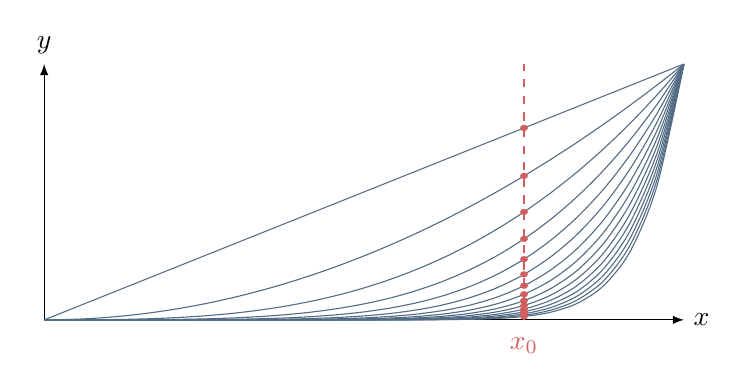
\begin{tikzpicture}[domain=0:1, scale=3.25, xscale=2.5]
      \draw[-latex] (0,0) -- (1,0) node [right] {$x$};
      \draw[-latex] (0, 0) -- (0,1) node [above] {$y$};
      \foreach \n in {1,...,15}
      {
         \draw[color=DarkBlue1] plot[smooth] (\x, {\x^\n});
         \fill[color=BrightRed1] (0.75, 0.75^\n) circle[radius=0.35pt, xscale=0.5];  
      }
      \draw[dashed, color = BrightRed1] (0.75, 0) -- (0.75,1);
      \draw[color=BrightRed1] node at (0.75, -0.1) {$x_0$}; 
   \end{tikzpicture}
\end{center}

Alors cette suite converge vers la fonction:
\[
   \begin{aligned}
      f : \icc{0}{1} &\longrightarrow \R\\
      x &\longmapsto \begin{cases}
         0 \text{ si } x < 1 \\
         1 \text{ sinon}
      \end{cases} 
   \end{aligned}
\]
On remarque un premier problème venant de cette définition, en effet les fonctions \(f_n\) sont toutes continues mais la limite n'est plus continue. Cela motive une notion de convergence plus \textbf{forte}.
\subsection*{\subsecstyle{Convergence uniforme{:}}}
On dit que \((f_n)\) \textbf{converge uniformément} vers \(f\) sur \(\R\) et on note \((f_n) \rightrightarrows f\) si et seulement si:
\[
   \forall \epsilon > 0 \; , \; \exists N \in \N \; , \; \forall n > N \; , \; \forall x \in \R \; ; \; |f_n(x) - f(x)| < \epsilon
\]
L'inversion des quantificateurs nous donne alors un unique seuil à partir duquel \(|f_n(x) - f(x)| < \epsilon\), en particulier, on peut alors montrer que cette notion de convergence équivaut à un criète plus pratique. En effet \((f_n)\) converge uniformément vers \(f\) si et seulement si:
\customBox{width = 4cm}{
   \(
      \vectNorm{f_n - f}_\infty^\R \rightarrow 0
   \)
}
On rapelle que la norme infini est définie par:
\[
   \vectNorm{f_n - f}_\infty^\R = \underset{x \in \R}{\sup}\left\{\left|f_n(x) - f(x)\right|\right\}
\]
Géométriquement, les boules pour cette norme consistent en des "tunnels" autour de la fonction centrale, et la convergence pour cette norme implique donc qu'à partir d'un certain rang, la suite de fonction se trouve toujours dans un tunnel arbitrairement petit.
\pagebreak

Par exemple la suite de fonctions \(f_n(x) = \frac{n + 2}{n}\sin(x)\) converge uniformément vers \(f: x \mapsto \sin(x)\) et graphiquement on a:

\begin{center}
   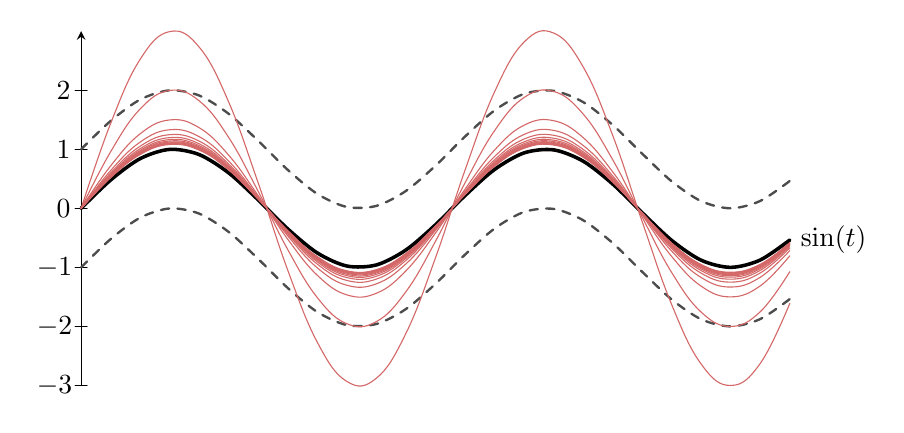
\begin{tikzpicture}[
      >=stealth,scale=0.75,line cap=round,
      bullet/.style={circle,inner sep=0.5pt,fill}
   ]
      \draw[->] (0,-3) -- (0, 3);
      \draw[] (-0.1,-3) -- (0.1, -3) node at (-0.45, -3) {$-3$};
      \draw[] (-0.1,0) -- (0.1, 0) node at (-0.3, 0) {$0$};
      \draw[] (-0.1,1) -- (0.1, 1) node at (-0.3, 1) {$1$};
      \draw[] (-0.1,2) -- (0.1, 2) node at (-0.3, 2) {$2$};
      \draw[] (-0.1,-2) -- (0.1, -2) node at (-0.45, -2) {$-2$};
      \draw[] (-0.1,-1) -- (0.1, -1) node at (-0.45, -1) {$-1$};

      \draw[color=black, domain=0:12, smooth, line width=0.45mm]   plot (\x,{sin(\x r)}) node[right] {$\sin(t)$}; 
      \draw[color=black!70,name path=A, domain=0:12, smooth, dashed, line width=0.3mm]   plot (\x,{sin(\x r) + 1}); 
      \draw[color=black!70,name path=B, domain=0:12, smooth, dashed, line width=0.3mm]   plot (\x,{sin(\x r) - 1}); 
      \foreach \n in {1, 2, 4, 6, 8, 10, 12, 14, 16, 18, 20, 22, 24}
      {
         \draw[color=BrightRed1!95, domain=0:12] plot[smooth, tension=0.70] (\x, {(\n+2)/\n*sin(\x r)});
      }
   \end{tikzpicture}   
\end{center}
\subsection*{\subsecstyle{Propriétés de régularité conservées{:}}}
Soit \((f_n)\) une suite de fonction qui converge uniformément vers \(f\), la valeur de notre définition est mise en lumière par les propriétés suivantes:
\begin{itemize}
   \item Si chaque \(f_n\) est \textbf{bornée}, alors \(f\) est \textbf{bornée}.
   \item Si chaque \(f_n\) est \textbf{continue}, alors \(f\) est \textbf{continue}.   
   \item Si chaque \(f_n\) est \textbf{uniformément continue}, alors \(f\) est \textbf{uniformément continue}.
\end{itemize}
\begin{center}
   \textit{Beaucoup de propriétés de régularité passent à la limite uniforme.}
\end{center}
Néanmoins le cas de la dérivabilité est plus subtil, en effet considéront la suite \((f_n)\) définie par \(f_n(x) = x^{1+\frac{1}{2n+1}}\), alors elle est bien définie et dérivable\footnote[1]{Remarquer que \(2n+1\) est toujours impair, donc on prends des racines n-ièmes impaires.} sur \(\R\), mais on a:
\begin{center}
   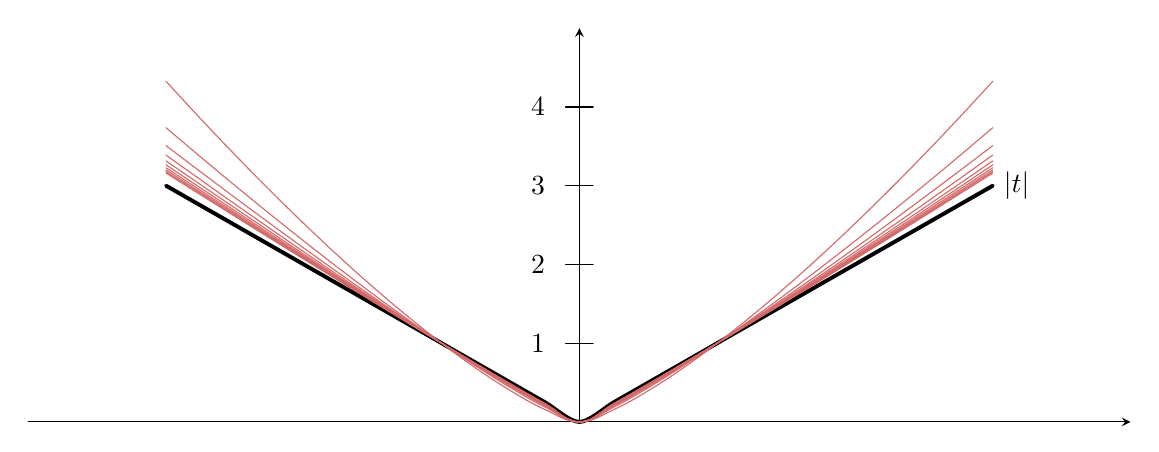
\begin{tikzpicture}[
      >=stealth,xscale=1.75, yscale=1,line cap=round,
      bullet/.style={circle,inner sep=0.5pt,fill}
   ]
      \draw[->] (0,0) -- (0, 5);
      \draw[->] (-4,0) -- (4,0);
      \draw[] (-0.1,1) -- (0.1, 1) node at (-0.3, 1) {$1$};
      \draw[] (-0.1,2) -- (0.1, 2) node at (-0.3, 2) {$2$};      
      \draw[] (-0.1,3) -- (0.1, 3) node at (-0.3, 3) {$3$};
      \draw[] (-0.1,4) -- (0.1, 4) node at (-0.3, 4) {$4$};

      \draw[color=black, domain=-3:3, smooth, line width=0.5mm]   plot (\x,{abs(\x)}) node[right] {$|t|$}; 
      \foreach \n in {1,..., 10}
      {
         \draw[color=BrightRed1!95, domain=-3:3] plot[smooth, tension=0.70] (\x, {\x*\x^(1/(2*\n+1))});
      }
   \end{tikzpicture}   
\end{center}
\[
   (f_n) \rightrightarrows f \text{ pour } f : x \mapsto |x|
\]
Et donc en particulier on a exhibé une suite de fonctions dérivables donc la limite uniforme \textbf{n'est pas dérivable} en un point.
\subsection*{\subsecstyle{Limites en un point{:}}}
On peut généraliser le résultat sur la continuité à un résultat sur les limites, en effet si \((f_n)\) est une suite de fonctions qui converge uniformément vers \(f\) et telles que \(f_n(x)\) admette une limite un un point \(a\), alors on a \textbf{le théorème d'interversion} suivant:
\customBox{width=7.5cm}{
   \[
      \lim_{n \rightarrow +\infty}\left(\lim_{x \rightarrow a} f_n(x)\right) = \lim_{x \rightarrow a}\left(\lim_{n \rightarrow +\infty} f_n(x) \right)
   \]
}
\subsection*{\subsecstyle{Intégrabilité{:}}}
On peut alors aussi montrer que si \((f_n)\) est une suite de fonction intégrables qui convergent uniformément vers \(f\), alors \(f\) est intégrable et on a \textbf{le théorème d'interversion} suivant:
\customBox{width=7cm}{
   \[
      \lim_{n \rightarrow +\infty}\int_{a}^{b} f_n(t) d t = \int_{a}^{b} \lim_{n \rightarrow +\infty} f_n(t) d t
   \]
}
\subsection*{\subsecstyle{Retour sur la dérivabilité{:}}}
Aprés avoir montré que la dérivabilité ne passe pas à la limite uniforme, on veut néanmoins trouver des critères permettant de trouver la dérivée d'une limite d'une suite de fonctions, on considère alors une suite de fonctions \((f_n)\) toutes dérivables qui converge simplement vers une fonction \(f\), et on suppose en outre que \textbf{la suite des dérivées \((f_n')\) converge uniformément}.\<

Alors \((f_n)\) converge uniformément vers \(f\) et cette dernière est dérivable de dérivée:
\[
   f'(x) = \lim_{n \rightarrow +\infty} f_n'(x)
\] 
On note alors que pour que la dérivabilité passe à la limite, il nous faut la convergence uniforme de la suite des dérivées \footnote[1]{Les conditions présentées sont suffisantes mais pas nécessaires pour permettre de gagner en clarté d'exposition. Pour être plus précis, il suffit que la suite converge simplement en un seul point}.
\subsection*{\subsecstyle{Approximations uniformes{:}}}
On se demande maintenant quand peut-on dire qu'une fonction continue est limite uniforme d'une suite de fonctions. Le \textbf{théorème de Weierstrass} nous donne alors une réponse forte:
\begin{center}
   \textbf{Toute fonction continue sur un segment est limite uniforme d'une suite de fonctions polynomiales.}
\end{center}
\chapter*{\chapterstyle{VI --- Séries de fonctions}}
\addcontentsline{toc}{section}{Séries de fonctions}
On appelle série de fonctions de terme général \(f_n\) la suite \(S_n\) des \textbf{sommes partielles} des termes de la suite de fonctions \((f_n)_{n\in\N}\), plus formellement, on a:
\[
   S_n = \sum_{k=0}^{n} f_k   
\]
Ce chapitre consistera en l'étude de la convergence de ces cas particuliers de suite de fonctions, ansi que de la qualité de cette convergence, comme dans le cas des suites de fonctions usuelles. 
\subsection*{\subsecstyle{Convergence simple{:}}}
On définit de la même manière que pour une suite de fonctions classiques la \textbf{convergence simple} d'une série de fonctions, il suffit alors, comme dans le cas d'une suite de fonction classique, d'effectuer la même étude en \textbf{fixant} \(x_0 \in \R\) et en étudiant la limite de la série \textbf{numérique}:
\[
   S_n(x_0) = \sum_{k=0}^{n} f_k(x_0)   
\]
On remarquera alors le même défaut de perte de régularité à la limite que dans le cas des suites de fonctions, cela était prévisible, les séries ne sont en effet qu'un cas particulier des suites. Cela motive à nouveau la notion de convergence uniforme.

\subsection*{\subsecstyle{Convergence uniforme{:}}}
On définit de la même manière que pour une suite de fonctions classiques la \textbf{convergence uniforme} d'une série de fonctions, il suffit alors, comme dans le cas d'une suite de fonction classique, ie il suffit de montrer que:
\[
   \vectNorm{S_n - S}_\infty^\R \longrightarrow 0
\]
Alors pour les mêmes interprétations que dans le cas des suites de fonctions, on aura une notion de convergence plus forte.

\subsection*{\subsecstyle{Propriétés de régularité conservées{:}}}
Soit \((S_n)\) une série de fonction qui converge uniformément vers \(S\), alors comme cas particulier de suite de fonction, on a évidemment à nouveau:
\begin{itemize}
   \item Si chaque \(S_n\) est \textbf{bornée}, alors \(S\) est \textbf{bornée}.
   \item Si chaque \(S_n\) est \textbf{continue}, alors \(S\) est \textbf{continue}.   
   \item Si chaque \(S_n\) est \textbf{uniformément continue}, alors \(S\) est \textbf{uniformément continue}.
\end{itemize}
\begin{center}
   \textit{Beaucoup de propriétés de régularité passent à la limite uniforme.}
\end{center}
Néanmoins comme précédemment, on montre facilement que la dérivabilité ne passe pas si simplement à la limite uniforme, et on a alors la même condition de dérivabilité de la limite que pour les suites donnée au chapitre précédent.\<

On peut aussi à nouveau généraliser la conservation de la continuité par la conservation de la limite, comme dans le chapitre précédent ainsi que la conservation de l'intégrabilité et on a donc:
\[
   \lim_{n \rightarrow +\infty}\int_{a}^{b} S_n(t) d t = \int_{a}^{b} \lim_{n \rightarrow +\infty} S_n(t) d t
\]
\pagebreak
\subsection*{\subsecstyle{Convergence normale{:}}}
Finalement, dans le cas des séries de fonctions, on définit un dernier mode de convergence plus fort appelé \textbf{convergence normale} et on dira qu'une série de fonction converge normalement si et seulement si la série numérique suivante converge:
\[
   \sum_{k=0}^{n} \vectNorm{f_k}_\infty^\R   
\]
L'intérèt de cette nouvelle définition et que la convergence normale implique la convergence uniforme, ce qui nous donne donc une condition suffisante trés pratique pour montrer la convergence uniforme d'une série de fonctions.

\subsection*{\subsecstyle{Fonctions définies par une série{:}}}
On peut alors définir des nouvelles fonctions par la limite de séries de fonctions, et dont le domaine de définition sera donc le domaine de convergence de la série. Une telle fonction sera de la forme:
\customBox{width=6cm}{
   \(f(z): z \mapsto \sum_{n=0}^{+\infty} f_n(z)\)
}
\underline{Exemple:} On peut définir la \textbf{fonction exponentielle}, définie sur \(\R\) par:
\[
   \exp: x \mapsto \sum_{n=0}^{+\infty} \frac{x^k}{k!}
\]
C'est d'ailleurs même un exemple de \textbf{série entière} qui seront les objets d'étude du chapitre suivant.
\chapter*{\chapterstyle{VI --- Séries Entières}}
\addcontentsline{toc}{section}{Séries Entières}
On se propose dans ce chapitre d'étudier des séries de fonctions particulières au comportement particulièrement intéressant, qui s'appeleront \textbf{séries entières} et on appelle série entière de terme général \(a_nz^n\) une série de fonctions \(S_n\) de variable complexe\footnote[1]{On définit ici les séries entières dans la plus grande généralité mais on se restreindra assez vite au cas réel.} \(z\) de la forme:
\[
   S_n(z) = \sum_{k=0}^{n} a_nz^n 
\]
L'étude de ce type de série permet alors de généraliser le concept de \textbf{polynôme} (définis comme sa suite (finie) de coefficients), en une notion de polynôme dont la suite de coefficients est infinie. Il faut alors déterminer dans quels cas ces séries convergent (si elle convergent) et étudier la qualité de cette convergence.

\subsection*{\subsecstyle{Convergence{:}}}
On s'intéresse tout d'abord à la convergence simple de ces séries, et le premier résultat particulièrement intéressant est le suivant, si on suppose que la série converge pour un certain \(z_0\), alors on peut montrer que:
\[
   \forall z \in \mathcal{D}(0, z_0) \; ; \; S_n(z) \textbf{ converge aussi }.
\]
Géométriquement, cela signifie que les domaines de convergence de ces séries ont des propriétés de symétries trés intéressantes, elle convergent sur ce qu'on appelera \textbf{un disque de convergence} centré en \(0\) et dans le cas réel qui nous intéressera, sur un intervalle de la forme \(\ioo{-R}{R}\) pour un certain réel \(R\) qu'on appelera alors \textbf{rayon de convergence de la série}.

\subsection*{\subsecstyle{Rayon de convergence{:}}}
Il reste alors à caractériser ce rayon de convergence pour savoir exactement sur quel domaine une série entière donnée converge, on précise tout d'abord la forme du rayon de convergence, c'est le réel donné par:
\[
   R := \sup \Bigl\{ |z| \; ; \; \sum_{k=0}^{n} a_nz^n \text{ converge } \Bigl\}   
\]
On simplifie ici l'étude en considérant le cas commun de séries telles que la limite de d'Alembert ou de Cauchy existe ou est infinie\footnote[2]{Dans le cas contraire (par exemple penser à \(a_n = sin(n)\)), on doit utiliser le "vrai" critère de Cauchy donné par:\[R:= \frac{1}{\limsup{\sqrt[n]{|a_n|}}}\]}, alors on applique le critère de Cauchy à la série et on obtient alors des informations sur le rayon de convergence:
\[
   |x| < \lim_{n \rightarrow +\infty}\sqrt[n]{|a_n|}^{-1} = \lim_{n \rightarrow +\infty} \frac{|a_n|}{|a_{n+1}|} = l
\]
Alors dans ce cas on a \(R := l\) et on a aussi la propriété de régularité trés forte suivante:
\begin{center}
   \textbf{Une série entière converge normalement sur tout compact strictement inclu dans le disque de convergence.}
\end{center}
\subsection*{\subsecstyle{Propriétés algébriques{:}}}
On se donne deux séries entières \(\sum a_nz_n, \sum b_nz_n\) de rayons de convergences respectifs \(R_a, R_b\), alors pour tout \(|z| < \min\{R_a, R_b\}\), on a:
\[
   \begin{cases}
      \left(\sum a_nz_n\right) + \left(\sum a_nz_n\right) \textbf{ converge }\\
      \left(\sum a_nz_n\right)\left(\sum b_nz_n\right) \textbf{ converge }
   \end{cases}
\]
Ce qui signifie simplement que le rayon de convergence de la somme ou du produit est \textbf{au moins supérieur} au minimum des rayons de convergence.

\subsection*{\subsecstyle{Régularité{:}}}
On s'intéresse maintenant à la régularité d'une fonction \(f\) définie par une série entière sur son disque de convergence, alors on peut montrer par les propriétés sur la convergence uniforme qu'elle est de classe \(\mathcal{C}^\infty\) sur son disque de convergence et on a donc:
\[
   f'(x) = \sum_{n=1}^{+\infty} na_nx^{n-1}  
\]
Et plus généralement, on peut \textbf{dériver termes à termes} une série entière et on a:
\[
   f^{(k)}(x) = \sum_{n=k}^{+\infty} n(n-1)\ldots(n-(k-1))a_nx^{n-k}  
\]
Par ailleurs, on peut alors montrer une condition nécéssaire sur les coefficients de la série, en effet on a:
\[
   a_n = \frac{f^n(0)}{n!}   
\]
Ce qui permet alors de démontrer que si une fonction donnée peut s'écrire comme une série entière alors, cette écriture est bien \textbf{unique}. 
\subsection*{\subsecstyle{Fonctions analytiques{:}}}
On considère maintenant le problème inverse, on se donne une fonction \(f\) et on se demande si elle peut s'écrire comme une série entière centrée en un point \(a \in \C\), ie si il existe une série entière \(\sum_{n=0}^{+\infty} a_nz^n\) et un rayon de convergence \(R\) tels\footnote[1]{Cela revient par translation à trouver une série entière au sens défini plus haut telle que:
\[
   g(z) = f(z + a) = \sum_{n=0}^{+\infty} a_nz^n
\]} que:
\[
   \forall z \in \mathcal{D}(a, R) \; ; \; f(z) = \sum_{n=0}^{+\infty} a_n(z - a)^{n}  
\]
Si c'est le cas, on dira alors que la fonction est \textbf{analytique} en \(a\), et on dira simplement qu'elle est analytique si elle est analytique en tout points de son domaine de définition. Par exemple la fonction exponentielle est analytique.\<

Cette propriété est plus forte encore que d'être de classe \(\mathcal{C}^\infty\), en effet il existe des fonctions de cette classe qui ne sont pas analytiques, l'exemple canonique étant \(x \mapsto \exp(-\frac{1}{x^2})\)

\subsection*{\subsecstyle{Applications{:}}}
L'application principale des fonctions analytiques est la résolution des équations fonctionelles, différentielles par exemple. En effet, étant donnée un équation différentielle \(E\), on peut tenter de chercher des solutions sous la forme d'une fonction analytique, ce qui permet souvent de simplifier les calculs par unicité du développement en série entière. En effet, il suffit alors souvent d'identifier les coefficients.\<

\uline{Exemple:} On cherche à résoudre l'équation \(f(x) = f'(x)\), en particulier on va chercher ses solutions analytiques, on a donc l'équation:
\[
   \sum_{n=0}^{+\infty}a_nx^n = \sum_{n=1}^{+\infty}na_nx^{n-1} = \sum_{n=0}^{+\infty}(n+1)a_{n+1}x^{n}
\]
Par identification des coefficients, on trouve donc que \(a_0\) est un réel quelconque et que \(a_n = na_{n-1}\), ie que \(a_n = \frac{a_0}{n!}\), et finalement on peut donc identifier les fonctions de la forme \(f(x) = ce^x\) avec la série entière obtenue.
\chapter*{\chapterstyle{VI --- Séries de Fourier}}
\addcontentsline{toc}{section}{Séries de Fourier}
On se propose dans ce chapitre d'étudier des séries de fonctions particulières, qui sont à la base de \textbf{l'analyse harmonique} qui vise à étudier les signaux périodiques ou non et à le représenter comme \textbf{superpositions de signaux élémentaires}.

\subsection*{\subsecstyle{Polynômes trigonométriques{:}}}
On définit pour se faire les \textbf{polynômes trigonométriques} à coefficients complexes\footnote[1]{On peut alors les définir algébriquement comme étant \(\C[exp(it)]\) et montrer que ces polynômes on bien une structure d'anneau (et même d'algèbre) de manière analogue aux polynômes usuels.}, qui sont les fonctions de la forme suivante:
\[
   f(x) = \sum_{k=-n}^{n} e^{ik\omega t} \underset{not.}{=} \sum_{k = 0}^{n} c_k e^{ik\omega t} + c_{-k}e^{-ik\omega t}    
\]
On a ici \(c_n\) deux suites de coefficients complexes et \(\omega\) un réel. Plus généralement, gràce\footnote[2]{En exprimant \(e^{ik\omega x}\) sous forme trigonométrique, on montre facilement que \(\begin{cases} a_n = c_n + c_{-n} \\ b_n = i(c_n - c_{-n}) \end{cases}\)} aux formules d'Euler, on peut montrer que tout polynôme trigonométrique peut s'écrire graàce aux fonctions trigonométriques classiques par:
\[
   S = \frac{a_0}{2} + \sum_{k=1}^{n} a_kcos(k\omega t) + b_ksin(k\omega t)   
\]
On peut alors facilment voir que ces polynômes sont \(\frac{2\pi}{\omega}\)-périodiques. On généralise alors à nouveau ce concept de polynômes trigonométriques au concept de \textbf{séries trigonométriques} qui, sous réserve d'existence, seront de la forme:
\[
   S = \sum_{k=-\infty}^{\infty} e^{ik\omega t} = \frac{a_0}{2} + \sum_{k=1}^{\infty} a_kcos(k\omega t) + b_ksin(k\omega t)
\]
La grande idée de Fourier est de considérer une fonction périodique \(f\) et d'essayer de décomposer cette fonction en une série trigonométrique, et donc de déterminer les suites de coefficients \(a_n, b_n, c_n\) adaptées à \(f\).

\subsection*{\subsecstyle{Coefficients de Fourier{:}}}
On considère maintenant une fonction \(2\pi\)-périodique \(f\) telle qu'elle soit développable en série de Fourier, ie que la série trigonométrique suivante converge uniformément:
\[
   f(x) = \sum_{n = -\infty}^{+\infty} c_n e^{inx}   
\]
Alors on cherche la forme du coefficient \(c_m\) de cette décomposition pour \(m \in \Z\), on transforme alors l'égalité en:
\[
   f(x)e^{-imx} = \sum_{n = -\infty}^{+\infty} c_n e^{ix(n - m)}
\]
L'idée étant alors de remarquer que si on intègre cette relation sur une période, on obtient:
\begin{align*}
   \int_{0}^{2\pi} f(x)e^{-imx} d x &= \int_{0}^{2\pi} \sum_{n = -\infty}^{+\infty} c_n e^{ix(n - m)} d x \\
   & = \sum_{n = -\infty}^{+\infty} c_n \int_{0}^{2\pi} e^{ix(n - m)} d x\\
   & = 2\pi c_m
\end{align*}
En effet toutes les intégrales sont nulles pour \(n \neq m\), ce qui nous donne donc l'expression générale des coefficients \footnote[1]{Avec le premier coefficient donné par \(c_0\), c'est la valeur moyenne de la fonction sur une période.} de Fourier de \(f\):
\[
   c_n(f) = \frac{1}{2\pi} \int_{0}^{2\pi} f(x)e^{-inx} d x
\]
On note souvent \(c_n(f)\) simplement \(c_n\) quand il n'y a pas de confusions possibles. Alors gràce aux relations explicitées dans la note de bas de page ci-dessus, on peut retrouver les coefficients \(a_n, b_n\) si nécéssaires.

\subsection*{\subsecstyle{Propriétés des coefficients{:}}}
On peut alors montrer plusieurs propriétés trés pratiques des coefficients de Fourier:
\begin{itemize}
   \item Si \(f\) est \textbf{paire} alors on a pour tout \(n\) que \(c_n = c_{-n}\)
   \item Si \(f\) est \textbf{impaire} alors on a pour tout \(n\) que \(c_n = -c_{-n}\).
\end{itemize}
Ces propriétés permettent souvent de calculer plus facilement les coefficients de Fourier.

\subsection*{\subsecstyle{Théorème de Jordan-Dirichlet{:}}}
Il reste maintenant à comprendre quelles sont les conditions pour qu'une fonction \(2\pi\)-périodique soit développable en série de Fourier on considère donc les coefficients construits plus haut et on s'intéresse à la convergence de la série :
\[
   \sum_{n = 1}^{+\infty} a_n\cos(nx) + b_n\sin(nx) = \sum_{n = -\infty}^{+\infty} c_ne^{inx}   
\]
C'est l'objet du \textbf{théorème de Jordan-Dirichlet} qui affirme que:
\begin{itemize}
   \item Si \(f\) est \(C^1\) par morceaux, alors sa série de Fourier converge vers \(\frac{f(x^+) + f(x^-)}{2}\).
   \item Si \(f\) est de plus \textbf{continue} alors sa série de Fourier converge \textbf{normalement} vers \(f\).
\end{itemize}
Ceci signifie alors informellement le résultat principal de ce chapitre:
\begin{center}
   \textit{Si une fonction périodique est suffisement régulière, elle est décomposable en série de Fourier.}
\end{center}

\subsection*{\subsecstyle{Harmoniques{:}}}
Pour une fonction périodique donnée qui serait développable en série de Fourier, on définit sa \textbf{fréquence} par la quantité \(F = \frac{1}{T}\) on remarque alors qu'elle se décompose sous la forme d'une somme de fonctions trigonométriques telles que \textbf{leurs fréquences est multiple de la fréquence de la fonction}, on appelle alors la fréquence de la fonction \textbf{fréquence fondamentale} ou \textbf{première harmonique}, et on définit la \textbf{n-ième harmonique} par:
\[
   H_n(f) : x \longmapsto c_n(f)e^{in\omega x} + c_{-n}(f)e^{-in\omega x}  
\]
On trouve alors directement une autre expression de la série de Fourier équivalente aux précédentes:
\[
   S_n(f) = c_0(f) + \sum_{k=1}^{n} H_k(f)
\] 
Cette expression peut être pratique car elle permet de passer rapidement de la série de Fourier complexe à la série de Fourier réelle, en appairant les termes d'indices opposés et en utilisant les formules d'Euler.
\pagebreak
\subsection*{\subsecstyle{Formule de Parseval{:}}}
Enfin, une formule fondamentale de la théorie des séries de Fourier est celle de \textbf{Parseval}, on définit d'abord le produit scalaire suivant sur l'espace des fonctions \(T\)-périodiques:
\[
   \dotproduct{f}{g} := \frac{1}{T}\int_T f(t)\overline{g(t)} d t   
\]
On considère alors la famille suivante de vecteurs suivante:
\[
   \mathscr{B} = (e^{in\omega x})_{n \in \Z}
\]
Alors cette famille est \textbf{orthogonale} donc libre, et elle engendre l'espace des polynômes trigonométriques, gràce à cette approche, on a alors que:
\[
   c_n(f) = \dotproduct{f}{e_n}
\]
On peut alors montrer une généralisation du \textbf{théorème de Pythagore} dans les espaces de dimension infinie dotés d'une base \(\mathscr{B}\) par:
\[
   \vectNorm{x}^2 = \sum_{e_i \in \mathscr{B}}\dotproduct{x}{e_i}^2
\]
Et donc dans ce cas particulier, on obtient l'égalité suivante:
\[
   \frac{1}{T} \vectNorm{f}^2 = \frac{1}{T} \int_{0}^{2\pi} |f(t)|^2 d t = \sum_{n=-\infty}^{+\infty} |c_n|^2 = \frac{a_0^2}{4} + \frac{1}{2} \sum_{n=1}^{+\infty} a_n^2 + b_n^2
\]
On peut en donner une interprétation physique assez évocatrice, en effet ce théorème se résume à dire que:
\begin{center}
   \textit{L'énergie de la fonction periodique est exactement décrite par la somme des énérgies des différentes harmoniques.}
\end{center}
Cette formule permet alors de calculer de nouvelles sommes si l'intégrale est facile à calculer, par exemple on peut facilement\footnote[1]{Il faut considèrer la fonction \(2\pi\) périodique égale à \(x\) sur \(\ico{-\pi}{\pi}\) puis appliquer Parseval} résoudre le problème de Bâle et montrer:
\[
   \sum_{n=1}^{+\infty}\frac{1}{n^2} = \frac{\pi^2}{6}   
\]
\pagebreak

\subsection*{\subsecstyle{Exemples d'un développement {:}}}
On considère la fonction \(2-\pi\) périodique telle que:
\[
   f(x) = x^2-\pi^2 \text{ sur } \inticc{-\pi}{\pi}
\]
On remarque rapidement qu'elle est périodique et continue, elle est donc décomposable en série de Fourier, calculons ses coefficients:
\begin{flalign*}
   c_n(f) &= \frac{1}{2\pi} \int_{-\pi}^{\pi} f(t)e^{-int} d t\\
   &= \frac{1}{2\pi} \int_{-\pi}^{\pi} (t^2 - \pi^2)e^{-int} d t\\
   &= \frac{1}{2\pi} \left(\int_{-\pi}^{\pi} t^2e^{-int} d t - \pi^2\int_{-\pi}^{\pi}e^{-int} d t\right)\\
   &= \frac{1}{2\pi} \left(\int_{-\pi}^{\pi} t^2e^{-int} d t\right)\shorteqnote{(Intégrale d'une fonction impaire sur un intervalle symétrique.)} \\ 
   &= \frac{1}{-2n\pi i} \left(-2\pi^2i\sin(n\pi) - \frac{4\pi}{in}\cos(n\pi) + \frac{4}{in^2}\sin(n\pi)\right) \shorteqnote{(Aprés 2 IPP et utilisation des formules d'Euler.)}\\
   &= \frac{2\cos{n\pi}}{n^2} \shorteqnote{(Car \(\sin(n\pi)\) est nul)}\\
   &= \frac{2(-1)^n}{n^2}
\end{flalign*}
Aussi le premier coefficient est donné par:
\begin{flalign*}
   c_0(f) &= \frac{1}{2\pi} \int_{-\pi}^{\pi} t^2 - \pi^2 d t \\
   &= \frac{-2\pi^2}{3}
\end{flalign*}

Finalement, on calcule les harmoniques:
\[
   H_n(f) : x \longmapsto c_n(f)e^{inx} + c_{-n}(f)e^{-inx} = \frac{2(-1)^n}{n^2} (e^{inx} + e^{-inx}) = \frac{4(-1)^n}{n^2}cos(nx)
\]
Enfin on a donc le développement en série de Fourier donné par:
\[
   S(f) = \frac{-2\pi^2}{3} + \sum_{n=1}^{+\infty} \frac{4(-1)^n}{n^2}cos(nx)
\]
\subsection*{\subsecstyle{Application au calcul d'une somme {:}}}
D'aprés l'égalité de Parseval, on a alors que:
\[
   \frac{1}{2\pi}\int_{-\pi}^{\pi}|f(t)|^2 d t = \sum_{-\infty}^{+\infty} |c_n(f)|^2 = \frac{4\pi^4}{9} + 2\sum_{n=1}^{+\infty} |c_n(f)|^2 = \frac{4\pi^4}{9} + 2\sum_{n=1}^{+\infty} \frac{4}{n^4}
\]
Aussi on a:
\[
   \frac{1}{2\pi}\int_{-\pi}^{\pi}|f(t)|^2 d t = \frac{1}{2\pi}\int_{-\pi}^{\pi}(x^2 - \pi^2)^2 d t = \frac{8\pi^4}{15}
\]
Donc finalement on trouve que:
\[
   \sum_{n=1}^{+\infty} \frac{8}{n^4} = \frac{8\pi^4}{15} - \frac{8\pi^4}{9} = \frac{4\pi^4}{45}
\]
Et donc on a réussi à calculer la somme suivante:
\[
   \sum_{n=1}^{+\infty} \frac{1}{n^4} = \frac{\pi^4}{90}
\]

   \pagebreak   
   
   \addcontentsline{toc}{chapter}{Analyse Vectorielle} % REVAMP vu que j'ai refactor les limites abstraites
   \chapter*{\chapterstyle{VII --- Fonctions Vectorielles}} % 95 Fini
\addcontentsline{toc}{section}{Fonctions Vectorielles}

Dans ce chapitre nous étudions les propriétés analytiques et de régularité d'un ensemble plus général de fonctions, les \textbf{fonctions d'une variable à valeurs vectorielles} et plus précisément, on se concentrera principalement sur le cas des fonctions de \(\R\) dans \(\R^n\) muni de sa structure euclidienne si nécessaire.

\subsection*{\subsecstyle{Définition{:}}}
Soit \(A \subset \R\) une partie de \(\R\) et \((f_1, f_2, \ldots, f_n)  \in \mathcal{F}(A, \R)\) des fonctions réelles, alors on appelle \textbf{fonction vectorielle} les fonctions de la forme:
\[
   \begin{aligned}
      f: A &\longrightarrow \R^n\\
      t &\longmapsto (f_1(t), f_2(t), \ldots, f_n(t))
   \end{aligned}
\]
Dans le cas ou \(n = 2\) et si \(\)
\subsection*{\subsecstyle{Limites{:}}}
On caractérise alors \textbf{la limite d'une fonction vectorielle} \(f\) en un point \(a \in A\), par la limite par composante, ie on a:
\[
   \lim_{x \rightarrow a} f(t) = l \Longleftrightarrow \forall i \in \inticc{1}{n} \; ; \; \lim_{x \rightarrow a} f_i(t) = l_i  
\]
En particulier on remarque alors la simplicité de cette généralisation, les limites se calculent simplement composantes par composantes. On verra par la suite que cette définition permet bien d'étendre toutes les notions analytiques classiques.
\subsection*{\subsecstyle{Propriétés de régularité{:}}}
La limite étant caractérisée composantes par composantes, la notion de continuité s'étend naturellement composantes par composantes. Par ailleurs, on étends aussi la notion de dérivabilité et on dit qu'une fonction vectorielle \(f\) est \textbf{dérivable en a} si et seulement si la limite suivante existe:
\[
   \lim_{x \rightarrow a} \frac{f(x) - f(a)}{x - a}
\]
Ce qui équivaut alors à l'existence des limites correspondantes pour les composantes, et \(f\) est donc dérivable en \(a\) (par extension de classe \(\mathcal{C}^k\)) si chacune de ses composantes sont dérivables en \(a\) (ou de classe \(\mathcal{C}^k\) en \(a\)) et on note alors \(f'\) sa \textbf{dérivée} qui s'obtient simplement en dérivant composante par composante.\<

Géométriquement \(f'(t)\) représente \textbf{le vecteur tangent} (aussi appellé vecteur vitesse) à la courbe au temps \(t\). Dans \(\R^2\) par exemple:
\begin{center}
   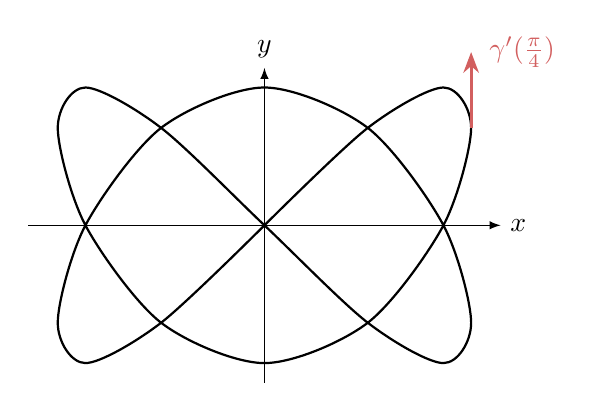
\begin{tikzpicture}[domain=-2:2, xscale=1.5]
      \tkzInit[xmin=-2,xmax=2,ymin=-2,ymax=2]
      \draw[-latex] (-2,0) -- (2,0) node [right] {$x$};
      \draw[-latex] (0, -2) -- (0,2) node [above] {$y$};
      \draw [thick] plot[color=DarkBlueX, variable=\t, domain=0:2*pi,smooth,thick] ({1.75*sin(2*\t r)},{1.75*sin(3*\t r)});   
      \draw[-Stealth, color=BrightRed1, line width=0.35mm] (1.75, 1.23) -- (1.75,2.2) node [right] {$\;\gamma'(\frac{\pi}{4})$};
   \end{tikzpicture}
\end{center}
\pagebreak
\subsection*{\subsecstyle{Propriétés non-conservées{:}}}
Néanmoins pour l cas de fonctions vectorielles, certaines propriétés ne sont pas conservées. En particulier, \textbf{le théorème de Rolle} n'est plus valable ainsi que le \textbf{le théorème des accroissements finis}.\footnote[1]{Evident aprés un dessin.}
Néanmoins, l'inégalité des accroissement finis reste valide et s'intérprète facilement cinématiquement:
\begin{center}
   \textit{Un point mobile qui se déplace à une vitesse instantanée inférieure à \(K\) sur un temps \(T\), se trouve au maximum à une distance \(KT\) de son point de départ.}
\end{center}
\subsection*{\subsecstyle{Dérivées de composées {:}}}
Soit \(f\) une fonction vectorielle dérivable, on peut alors se demander comment, étant donnée une application linéaire \(L\), se comporte la dérivée de la composée \(L \circ f\) et on montre alors à partir de la définition que:
\[
   (L(f))' = L(f')
\] 
On veut alors généraliser, et on considère deux fonctions vectorielles \(f, g\) dérivables, et une application bilinéaire \(B\), alors de la meme manière on peut montrer que:
\[
   B(f, g)' = B(f', g) + B(f, g')
\]
On peut alors y voir un analogue de la \textbf{règle du produit} pour la dérivation classique, en particulier si \(B = \dotproduct{\cdot}{\cdot}\), on a:
\[
   \dotproduct{f}{g}' = \dotproduct{f'}{g} + \dotproduct{f}{g'}
\]
Finalement, si on a une famille \(f_1, \ldots, f_n\) de fonctions vectorielles dérivables et une application multilinéaire \(M\), alors:
\[
   M(f_1, \ldots, f_n)' = M(f_1', \ldots, f_n) + \ldots + M(f_1, \ldots, f_n')
\]
En particulier si \(M = \det\), et pour les fonctions \(f, g, h\) on a:
\[
   \det(f, g, h)' = \det(f', g, h) + \det(f, g', h) + \det(f, g, h')  
\]
\subsection*{\subsecstyle{Intégration{:}}}
On peut alors raisonnablement penser que l'intégration sur un segment \(\icc{a}{b}\) se généralisera de la meme manière, et c'est le cas ! Si toutes les fonctions \((f_i)\) sont Riemann-intégrables sur le segment, alors on dira que la fonction \(f\) est Riemann-intégrable et on définit:
\[
   \int_{a}^{b} f(t) \d t = \left(\int_{a}^{b} f_1(t) \d t, \ldots, \int_{a}^{b} f_n(t) \d t\right)   
\]
En particulier cela donne lieu à une interprétation cinématique :
\begin{center}
   \textit{Si \(f\) est une fonction qui donne le vecteur vitesse d'un point mobile à un temps \(t\), alors son intégrale est le vecteur position associé.}
\end{center}
\subsection*{\subsecstyle{Points remarquables{:}}}
On peut par la suite définir plus d'outils analytiques sur cet ensemble de fonctions, mais pour cela il faut définir la notion d'arcs paramétré qui nécessite les définitions suivantes qui se ne sont que terminologie:
\begin{itemize}
   \item On appelle \textbf{point régulier} un point \(f(t)\) tel que \(f'(t) \neq 0\)
   \item On appelle \textbf{point critique} un point \(f(t)\) tel que \(f'(t) = 0\)
\end{itemize}
On appelle \textbf{point multiple} un point \(P\) de \(E\) tel qu'il existe \((t_0, \ldots, t_k)\) deux à deux distincts tels que \(\forall i \in \inticc{1}{k} \; f(t_i) = P\) et on appelle alors \textbf{multiplicité} l'entier \(k\).

\chapter*{\chapterstyle{VII --- Fonctions à plusieurs variables}}
\addcontentsline{toc}{section}{Fonctions à plusieurs variables}

Dans ce chapitre nous étudions les propriétés analytiques et de régularité d'un ensemble plus général de fonctions, les \textbf{fonctions d'un espace vectoriel normé dans un autre} et plus précisément, on se concentrera principalement sur le cas des fonctions de \(\R^n\) dans \(\R^p\).\<

Soit \(\mathcal{D}\) une partie de \(\R^n\) et \((x_1, \ldots, x_n) \in \mathcal{D}\), on considère alors la fonction:
\[
   \begin{aligned}
      f : \mathcal{D} \subseteq \R^n &\longrightarrow \R^p \\
      (x_1, \ldots, x_n) &\longmapsto (f_1(x), \ldots, f_p(x))
   \end{aligned}
\]
On dira alors que la fonction \(f_i\) est la i-ème application \textbf{composante} de \(f\).\+

\subsection*{\subsecstyle{Définitions{:}}}
On peut alors définir quelques notions de vocabulaire:
\begin{itemize}
   \item Si la fonction est à valeur scalaire, on dira que c'est \textbf{un champ de scalaires}.
   \item Si la fonction est à valeur vectorielles, on dira que c'est \textbf{un champ de vecteurs}.
\end{itemize}

\subsection*{\subsecstyle{Représentations{:}}}
On cherche alors à représenter de telles fonctions, on sait que dans le cas élémentaire des fonctions à une seule variable, on peut représenter le \textbf{graphe} d'une fonction \(f\) donné par:
\[
   \mathcal{G}_f := \bigl\{ (x, f(x)) \in \R^2 \; ; \; x \in \R \bigl\}   
\]
Dans le cas d'une fonction de plusieurs variables, on peut alors généraliser cette définition par:
\[
   \mathcal{G}_f := \bigl\{ (x, f(x)) \; ; \; x \in \R^n \bigl\}  
\]

De façon générale, le graphe d'une fonction de \(\R^n\) dans \(\R^p\) est un objet à \(n\) dimensions dans l'espace à \((n + p)\) dimensions (les points sont caractérisés par \(n\) paramètres, en termes
savants on dira qu'il s'agit d'une sous-variété de \(\R^{(n + p)}\) de dimension \(n\).\<

Si on considère par exemple une fonction de \(\R^2\) dans \(\R\), c'est alors une fonction qui à chaque point du plan associe une valeur numérique, qu'on peut alors représenter comme \textbf{une hauteur} et on obtient alors \textbf{une surface}, par exemple:

\begin{figure}
   \centering
   \vspace*{-0.5cm}
   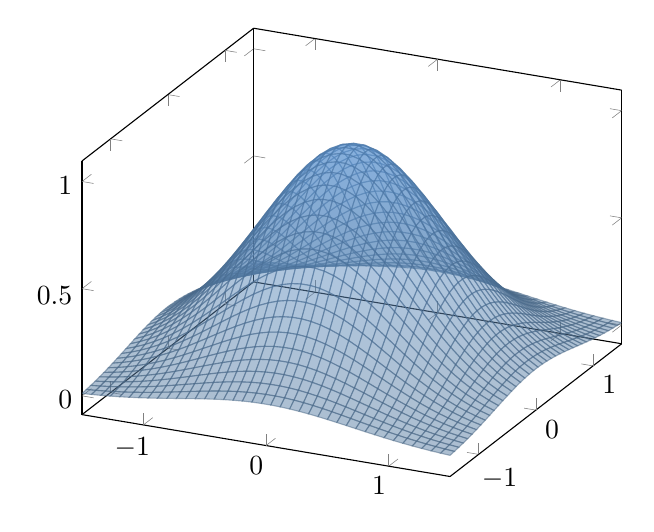
\begin{tikzpicture}
      \begin{axis}[domain=-1.5:1.5,y domain=-1.5:1.5, scale=1, colormap={custom}{color(0)=(DarkBlue3) color(1)=(BrightBlue1)}]
        \addplot3[draw=black, opacity=0.5, surf, samples=40] {exp(-x^2-y^2)};
      \end{axis}
    \end{tikzpicture}
   \captionsetup{labelformat=empty}
   \caption{Graphe de la fonction \(f : (x, y) \mapsto \exp(-x^2 - y^2)\)}
\end{figure}
\pagebreak

Dans le cas général néanmoins, il est plus difficile de représenter ce type de fonctions mais on peut par exemple s'inspirer des fonctions \(\C \rightarrow \C\) et utiliser la \textbf{couleur} comme 4-ème dimension de l'image. On peut aussi de manière heuristique représenter simplement le domaine de départ et/ou d'arrivée pour étudier le comportement de la fonction.

\subsection*{\subsecstyle{Cas des champs de vecteurs{:}}}
De manière générale, le caractère multidimensionnel de l'espace d'arrivée importe peu dans tout le chapitre qui va suivre, les notions analytiques étant définies à partir d'une limite, elles passeront aux composantes comme les notions évoquées au chapitre précédent.\<

Dans toute la suite on considèrera alors souvent le cas épuré de champs de scalaires et il est attendu d'adapter les résultat élémentaires aux cas à valeurs vectorielles.

\subsection*{\subsecstyle{Lignes de niveaux{:}}}
On considère une fonction \(f : \R^2 \rightarrow \R\), alors on appelle \textbf{ligne de niveau} associé à la valeur \(\lambda\) l'ensemble suivant:
\[
   L_\lambda := \Bigl\{ (x, y) \in \R^2 \; ; \; f(x, y) = \lambda \Bigl\}   
\]
C'est une courbe plane qui représente l'ensemble des points du plan ou la fonction prends une valeur fixée, tracer plusieurs lignes de niveaux permet alors d'obtenir des informations sur la fonction, par exemple:
\begin{figure}[h]
   \centering
   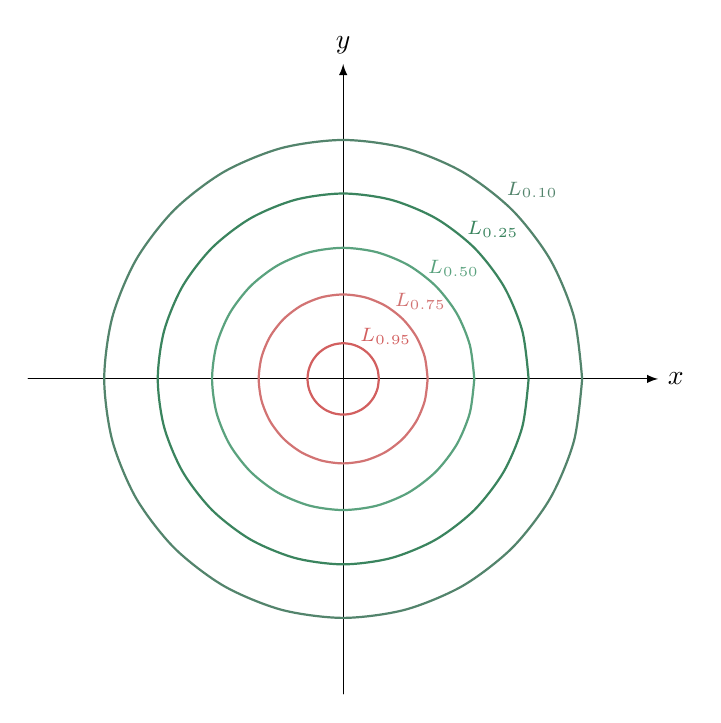
\begin{tikzpicture}[line cap=round, scale=2]
      \tkzInit[xmin=-2,xmax=2,ymin=-2,ymax=2]
      \draw[-latex] (-2,0) -- (2,0) node [right] {$x$};
      \draw[-latex] (0, -2) -- (0,2) node [above] {$y$};

      \draw [thick, color=BrightRed1] plot[domain=0:2*pi,variable=\t, line width=0.3mm, smooth] ({0.226480229573*cos(\t r)}, {0.226480229573*sin(\t r)});   
      \draw [thick, color=BrightRed2] plot[domain=0:2*pi,variable=\t, line width=0.3mm, smooth] ({0.536360021303*cos(\t r)}, {0.536360021303*sin(\t r)});   
      \draw [thick, color=DarkGreen1] plot[domain=0:2*pi,variable=\t, line width=0.3mm, smooth] ({0.83255461115*cos(\t r)}, {0.83255461115*sin(\t r)});   
      \draw [thick, color=DarkGreen2] plot[domain=0:2*pi,variable=\t, line width=0.3mm, smooth] ({1.17741002252*cos(\t r)}, {1.17741002252*sin(\t r)});   
      \draw [thick, color=DarkGreen3] plot[domain=0:2*pi,variable=\t, line width=0.3mm, smooth] ({1.51742712939*cos(\t r)}, {1.51742712939*sin(\t r)});    
      \draw node[color=BrightRed1] at (0.27, 0.27) {\scriptsize $L_{0.95}$};
      \draw node[color=BrightRed2] at (0.49, 0.49) {\scriptsize $L_{0.75}$};
      \draw node[color=DarkGreen1] at (0.7, 0.7) {\scriptsize $L_{0.50}$};
      \draw node[color=DarkGreen2] at (0.95, 0.95) {\scriptsize $L_{0.25}$};
      \draw node[color=DarkGreen3] at (1.2, 1.2) {\scriptsize $L_{0.10}$};
   \end{tikzpicture}
   \captionsetup{labelformat=empty}
   \caption{Lignes de niveau de la fonction \(f : (x, y) \mapsto \exp(-x^2 - y^2)\)}
\end{figure}

\subsection*{\subsecstyle{Changements de variables{:}}}
L'étude des fonctions à plusieurs variables va nous amener à étudier les \textbf{changements de variables} que nous allons définir:
\begin{center}
   \textbf{On appelle changement de variable tout \(\mathcal{C}^k\) difféomorphisme entre deux espaces.}
\end{center}
En particulier, on verra que le passage en coordonées polaires défini comme suite est bien un changement de variable et en tant que tel, il préserve les propriétés différentielles:
\[
   \begin{aligned}
      \phi : \R_+^* \times \ioo{-\pi}{\pi} &\longrightarrow \R^2 \backslash (\R_- \times \{0\})\\
      (r, \theta) &\longmapsto (r\cos(\theta), r\sin(\theta))
   \end{aligned}
\]

\chapter*{\chapterstyle{VII --- Limite \& Continuité}}
\addcontentsline{toc}{section}{Limite \& Continuité} 
Dans ce chapitre et comme vu dans le chapitre de Topologie, nous étudirons le concept de limite dans le cas d'une fonction à plusieurs variables, plus précisément, sauf exceptions, dans le cas d'un champ de scalaire. Dans les cas ou les généralités sont triviales, on utilisera sans vergogne l'exemple canonique d'une fonction \(f : \R^2 \rightarrow \R\). On rapelle qu'une limite d'une telle fonction se caractérise métriquement par la propriété:
\[
   \forall \epsilon >0 \; , \; \exists \lambda > 0 \; , \; \forall x \in \R^n \; , \; \vectNorm{x - a} < \lambda \implies |f(x) - l| < \epsilon
\]

\subsection*{\subsecstyle{Limites suivant une restriction{:}}}
Cette définition correspond bien à l'intuition \textit{topologique} de la notion de limite. En particulier, on peut alors montrer que si \(f\) tends vers \(l\) en \((a, b)\), alors en particulier si on considère un \textbf{chemin} de la forme:
\[
   \gamma : t \mapsto (\gamma_1(t), \gamma_2(t))   
\]
Et si ce chemin est tel qu'il passe par \((a, b)\) en \(t_0\), alors on a nécessairement:
\[
   \lim_{(x, y) \rightarrow (a, b)} f(x, y) = l \implies \lim_{t \rightarrow t_0} f(\gamma(t)) = l
\]
En particulier cela nous permet de construire une méthode pour démontrer la \textbf{non-existence de limite}, ie:
\begin{center}
   \textit{Si il existe deux chemins différents suivant lesquels la fonction admets deux limites différentes, alors elle n'admet pas de limite en ce point.}
\end{center}
\subsection*{\subsecstyle{Erreurs communes{:}}}
Cette définition correspond bien à l'intuition \textit{topologique} de la notion de limite. Néanmoins il faut remarquer les propriétés suivantes spécifiques aux fonctions à plusieurs variables:
\begin{itemize}
   \item Il est possible qu'une fonction admette une limite suivant plusieurs chemins, mais pas de limite.
   \item Il est meme possible qu'une fonction admette une limite suivant toutes les droites, mais pas de limite.
   \item De manière générale, admettre une limite sur plusieurs restrictions ne permet pas d'affirmer l'existence d'une limite.
\end{itemize}
\subsection*{\subsecstyle{Opérations{:}}}
Comme dans le cas des fonctions réelles, on peut alors démontrer les propriétés opératoires de la limite, en effet si on considère \(f, g\) deux champs scalaires qui admettent deux limites \(l_1, l_2\) en \(A \in \R^p\),alors on a les propriétés suivantes:
\begin{itemize}
   \item Le passage à la limite est \textbf{linéaire}.
   \item Le passage à la limite est \textbf{multiplicatif}.
   \item Le passage à la limite (non-nulle) d'une fonction localement non-nulle est \textbf{inversible}.
\end{itemize}
La première propriété se généralise aux champs vectoriels, mais pas les deux secondes bien évidemment, car les opérations en jeu (effectuées à l'arrivée) ne sont pas définies pour des vecteurs.\<

Enfin pour deux fonction qui sont composables, on a la propriété fondamentale suivante:
\begin{itemize}
   \item Le passage à la limite est compatible avec la \textbf{composition}.
\end{itemize}
\subsection*{\subsecstyle{Théorème d'encadrement {:}}}
On peut généraliser le théorème des gendarmes aux fonctions à plusieurs variables, en effet si on considère \(f, g, h\) trois fonctions telles que \(f(x, y) \leq g(x, y) \leq h(x, y)\) dans un voisinage de \((a, b)\) alors on a:
\[
   \lim_{(x, y) \rightarrow (a, b)} f(x, y) = \lim_{(x, y) \rightarrow (a, b)} h(x, y) = l \implies \lim_{(x, y) \rightarrow (a, b)} g(x, y) = l
\] 
\pagebreak
\subsection*{\subsecstyle{Passage en polaire {:}}}
Si on considère une fonction à deux variables, on peut exprimer \((x, y)\) en coordonées polaires, ie considérer la composée \(f(x, y) = f(r\cos(\theta), r\sin(\theta))\) et alors \(f\) tends vers \(0\) en \((0, 0)\) si et seulement si il existe une fonction \(g(r)\) telle que:
\[
   |f(r\cos(\theta), r\sin(\theta))| \leq g(r)
\]
Avec \(g(r)\) qui tends vers \(0\) quand \(r\) tends vers \(0\). \textbf{Attention} la fonction \(g\) ne doit plus dépendre de \(\theta\).
\subsection*{\subsecstyle{Continuité {:}}}
En tant que conséquence directe de la définition topologique, on dira alors qu'une fonction est \textbf{continue} en un point \(A\) si et seulement si:
\[
   \lim_{(x, y) \rightarrow A} f(x, y) = f(A)   
\]
Et toute les propriétés opératoires usuelles sont alors aisément démontrées. En particulier, on peut montrer que toutes les fractions rationnelles sont continues sur leur ensemble de définition, et donc tout les polynomes.

\chapter*{\chapterstyle{VII --- Cas des applications linéaires}}
\addcontentsline{toc}{section}{Cas des applications linéaires}
On s'intéresse dans ce chapitre à l'espace des applications linéaires \(\mathcal{L}(E, F)\) sur des espaces de dimensions finies. \<

C'est un exemple fondamental en analyse numérique et en mathématiques en général car les problèmes non-linéaires étant complexes, on se ramène souvent à la linéarisation d'un problème pour sa résolution. On cherche donc à affiner notre compréhension de la continuité de ces applications et poser quelques bases de topologie sur cet espace.
\subsection*{\subsecstyle{Continuité des applications linéaires {:}}}
Soit \(f : E \rightarrow F\) une application linéaire, alors on a le théorème fondamental suivant qui énonce que \(f\) est continue sur son domaine de définition si et seulement si elle vérifie une des conditions équivalentes suivantes:
\begin{itemize}
   \item Elle est continue en 0.
   \item Elle est bornée sur la boule unité.
   \item Elle est uniformément continue.
   \item Elle est lipschitzienne.
\end{itemize}
En particulier, muni des ces équivalences, on peut démontrer la propriétés fondamentale suivante:
\begin{center}
   \textbf{En dimension finie, toutes les applications linéaires sont continues.}
\end{center}

\subsection*{\subsecstyle{Normes d'opérateur {:}}}
On se donne une application linéaire et on munit \(E, F\) de deux normes \(\vectNorm{\cdot}_p, \vectNorm{\cdot}_q\), alors on apelle \textbf{norme d'opérateur} de \(f\) la quantité suivante:
\[
   \opNorm{f}_{p, q} = \sup_{\vectNorm{v}_p = 1} \vectNorm{f(v)}_q
\]
En outre par l'isomorphisme usuel entre l'espace des application linéaires et celui des matrices, on définit de même la \textbf{norme d'opérateur d'une matrice} par:
\[
   \opNorm{M}_{p, q} = \sup_{\vectNorm{V}_p = 1} \vectNorm{MV}_q
\]
On notera alors \(\opNorm{f}_{p}\) si la norme est la même au départ et à l'arrivée. On peut alors caractériser la continuité d'un opérateur par le fait que sa norme d'opérateur soit \textbf{finie}.


\subsection*{\subsecstyle{Normes matricielles {:}}}
On appelle \textbf{norme matricielle} toute norme sur un espace de matrice qui est aussi une \textbf{norme d'algèbre}, ie telle que:
\[
   \vectNorm{AB} \leq \vectNorm{A}\vectNorm{B}
\]
Par exemple, la norme de Frobenius est une norme matricielle. On a alors la propriété\footnote[1]{Pour montrer ceci il faut remarquer que pour tout \(x \in E\), on a \(\vectNorm{f(x)} = \opNorm{f}\vectNorm{x}\).} suivante:
\begin{center}
   \textbf{Toute norme d'opérateur est une norme matricielle.}
\end{center}

\subsection*{\subsecstyle{Normes usuelles {:}}}
On peut alors chercher à savoir à quoi correspondent les normes d'opérateurs induites par les normes usuelles, on peut montrer qu'elles vérifient:
\begin{itemize}
   \item La norme 1: \(\opNorm{A}_{1} = \max_{1 \leq j \leq n} \sum_{1 \leq i \leq n} |a_{i,j}|\), c'est le \textbf{maximum de la somme des colonnes.}
   \item La norme infinie: \(\opNorm{A}_{\infty} = \max_{1 \leq i \leq n} \sum_{1 \leq j \leq n} |a_{i,j}|\), c'est le \textbf{maximum de la somme des lignes.}
   \item La norme 2: \(\opNorm{A}_{2} = \sqrt{\rho({}^tAA)}\) où \(\rho(M)\) est le \textbf{rayon spectral} de \(M\).
\end{itemize}



\chapter*{\chapterstyle{VII --- Dérivées Directionnelles}}
\addcontentsline{toc}{section}{Dérivées Directionnelles} 
Dans ce chapitre nous essaierons de construire un concept de \textbf{dérivée} dans le cas d'une fonction à plusieurs variables, plus précisément, sauf exceptions, dans le cas d'un champ de scalaire. Dans les cas ou les généralités sont triviales, on utilisera sans vergogne l'exemple canonique d'une fonction \(f : \R^2 \rightarrow \R\)

\subsection*{\subsecstyle{Applications Partielles {:}}}
On considère une fonction de \(A \subseteq \R^p \rightarrow \R\) et un point \(a = (a_1, \ldots, a_n)\) \textbf{intérieur} à \(A\). Alors il existe un voisinage de \(a\) ou la fonction \textbf{réelle} suivante est bien définie, on l'appelle alors \textbf{i-ème application partielle} au point \(a\):
\[
   \begin{aligned}
      f_{x_i} : \R &\longrightarrow \R\\
      t &\longmapsto f(a_1, \ldots, t, \ldots, a_n)
   \end{aligned}
\]
\begin{center}
   \textit{Considèrer la i-ème application partielle, c'est fixer une direction et considèrer la courbe de \(f\) suivant cette direction.}
\end{center}
Géométriquement, on peut le voir comme l'interesection d'un plan parallèle à l'axe considéré et passant par \(a\), et l'application partielle est alors l'intersection de la courbe et du plan:
\begin{figure}[h]
   \centering
   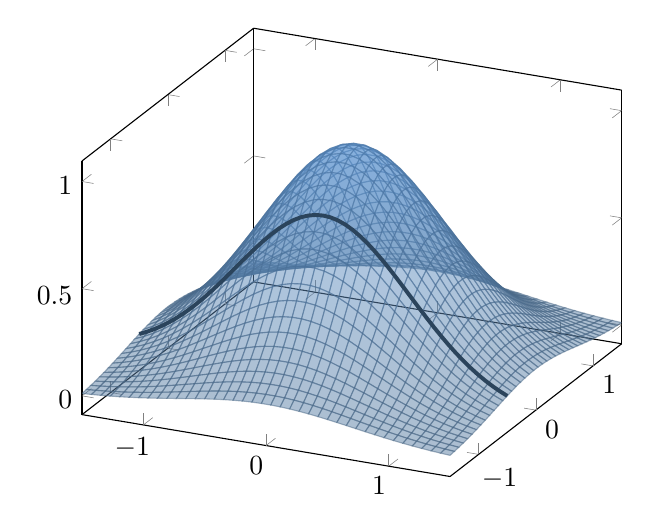
\begin{tikzpicture}
      \begin{axis}[domain=-1.5:1.5,y domain=-1.5:1.5, scale=1, colormap={custom}{color(0)=(DarkBlue3) color(1)=(BrightBlue1)}]
         \addplot3[draw=black, opacity=0.5, surf, samples=40] {exp(-x^2-y^2)};
         \addplot3[draw=DarkBlueX, line width = 0.5mm, samples=51, samples y=0,domain=-1.5:1.5,variable=\t]
         ({\t},{-0.5},{exp(-\t^2 - 0.5^2)});         
      \end{axis}
    \end{tikzpicture}
   \captionsetup{labelformat=empty}
   \caption{Application partielle \(f_x\) en \((0, -0.5)\) de \(f : (x, y) \mapsto \exp(-x^2 - y^2)\)}
\end{figure}
\subsection*{\subsecstyle{Dérivées Partielles {:}}}
On dira alors qu'une telle fonction \textbf{admet une i-ème dérivée partielle} au point \(a\) si et seulement si sa i-ème application partielle en \(a\) est dérivable en \(a_i\). On se ramène alors à l'étude de la dérivabilité d'une fonction \textbf{réelle}, ce qui ne pose pas de problème théorique. Dans ce cas, on notera alors:
\[
   \frac{\partial f}{\partial x_i}(a) = f_{x_i}'(a_i)   
\]
Si \(f\) admet une i-ème dérivée partielle sur un ouvert \(\mathcal{U}\) si et seulement si elle en admet en tout points de \(\mathcal{U}\) et on définit alors:
\[
   \begin{aligned}
      \frac{\partial f}{\partial x_i} : \mathcal{U} &\longrightarrow \R\\
      a &\longmapsto \frac{\partial f}{\partial x_i}(a_i)
   \end{aligned}
\]
On dira alors qu'un fonction à plusieurs variables est de classe \(\mathcal{C}^k\) en un point si elle admet toutes ses dérivées partielles en ce point et qu'elles y sont continues.
\pagebreak
\subsection*{\subsecstyle{Propriétés opératoires{:}}}
On peut montrer que la dérivation partielle est un \textbf{opérateur différentiel} agissant sur un espace de fonctions qui admettent des dérivées partielles, en particulier en utilisant les définitions précédentes et en notant \(\mathcal{D}_i(\R^n)\) l'espace des fonctions admettant une i-ème dérivée partielle, alors on peut définir:
\[
   \begin{aligned}
      \frac{\partial}{\partial x_i} : \mathcal{D}_i(\R^n) &\longrightarrow \mathcal{F}(\mathcal{U}, \R)\\
      f &\longmapsto \frac{\partial f}{\partial x_i}
   \end{aligned}
\]

C'est donc cet opérateur que nous appliquons à une fonction qui admet des dérivées partielles. En particulier, l'intéret de cette définition est alors de pouvoir affirmer les propriétés suivantes:
\begin{itemize}
   \item La dérivation partielle est \textbf{linéaire}.
   \item La dérivation partielle suit \textbf{la règle du produit}.
\end{itemize}
La première propriété se généralise aux champs vectoriels, mais pas la seconde bien évidemment, car les opérations en jeu (effectuées à l'arrivée) ne sont pas définies pour des vecteurs.\<

\underline{Exemple:} On considère les fonctions suivantes en un point \((x, y)\):
\[
   \begin{aligned}
      f : (x, y) &\longmapsto xy \quad\quad\quad g : (x, y) &\longmapsto x^2y
   \end{aligned}
\]
Alors on a\footnote[1]{\textbf{Attention:} Ici on fait l'abus de notation usuel d'utiliser deux fois la variable \(x\) qui ont deux sens différents, l'expression \(\partialD{fg}{x}\) signifie simplement qu'on dérive par rapport à la première variable (penser \(\partial_1(fg)\)) et \((x, y)\) représente le point d'évaluation de la dérivée partielle.)}:
\[
   \partialD{(fg)}{x}(x, y) = \partialD{f}{x}(x, y)g(x, y) + \partialD{g}{x}(x, y)f(x, y) = yx^2y + 2xyxy = 3x^2y^2
\]
On voit bien ici que la dérivée d'un produit n'a de sens que si on est dans le cas de (au moins un) champs scalaires !
\subsection*{\subsecstyle{Dérivée partielle d'une composée{:}}}
Le cas de la composée est plus subtil et on reviens temporairement au cas général des deux champs vectoriels suivants dont on supposera qu'ils admettent toutes leurs dérivées partielles partout:
\[
   \begin{aligned}
      g : \R^m &\longmapsto \R^n \quad\quad\quad f : \R^n &\longmapsto \R^p
   \end{aligned}
\]
On cherche à caculer la dérivée partielle par rapport à la \(i\)-ème variable de la fonction \(f \circ g\) au point \(a\), on peut alors montrer la formule suivante, appellée \textbf{chain rule}: 
\[
   \partialD{(f \circ g)}{x_i}(a) = \sum_{k=1}^{n} \partialD{g_k}{x_i}(a)\partialD{f}{x_k}(g(a))
\]
\underline{Exemple:} On considère un fonction \(f : \R^2 \rightarrow \R\) de classe \(\mathcal{C}^1\) et la fonction \(g\) de passage en polaire:
\[
   \begin{aligned}
      g : (r, \theta) &\longmapsto (r\cos(\theta), r\sin(\theta))
   \end{aligned}
\]
On se propose de calculer la première dérivée partielle de \(f \circ g\) au point \((r, \theta)\), on a alors:
\begin{flalign*}
   \partialD{(f \circ g)}{r}(r, \theta) 
   &= \partialD{g_1}{r}(r, \theta)\partialD{f}{x}(r\cos(\theta), r\sin(\theta)) + \partialD{g_2}{r}(r, \theta)\partialD{f}{y}(r\cos(\theta), r\sin(\theta))\\ 
   &= cos(\theta)\partialD{f}{x}(r\cos(\theta), r\sin(\theta)) + sin(\theta)\partialD{f}{y}(r\cos(\theta), r\sin(\theta))
\end{flalign*}
\subsection*{\subsecstyle{Dérivées partielles d'ordre supérieur {:}}}
La i-ème dérivée partielle de \(f\) étant à nouveau une fonction de \(n\) variables, on peut alors considèrer ses dérivées partielles. On définit les dérivées partielles secondes de \(f\) (si elles existent), notées:
\[
   \frac{\partial^2 f}{\partial x_i \partial x_j}(a)   
\]
Et par récurrence les dérivées partielles d'ordre \(k\) par:
\[
   \frac{\partial^k f}{\partial x_{i_1} \ldots \partial x_{i_k}}(a)
\]
Et on se pose alors la question de l'importance de \textbf{l'ordre de dérivation} et de manière générale, on peut alors montrer que l'ordre d'application de l'opérateur compte, ie que:
\[
   \frac{\partial^2 f}{\partial x_j \partial x_i}(a) \neq \frac{\partial^2 f}{\partial x_i \partial x_j}(a)
\]
Mais le théorème de Schwarz donne alors une condition suffisante pour que l'ordre ne compte pas:
\begin{center}
   \textbf{Si les dérivées partielles sont toutes continues en un point, alors l'ordre de dérivation n'importe pas.}
\end{center}
\subsection*{\subsecstyle{Dérivées Directionnelles {:}}}
Si on considère les dérivées partielles d'une fonction \(f\), qu'on note \(a = (x_1, \ldots, x_n)\) le point d'étude et \((e_i)\) la base canonique, on peut alors les caractériser par:
\[
   \frac{\partial f}{\partial x_i}(a) = \lim_{h \rightarrow 0} \frac{f(a + he_i) - f(a)}{h}
\] 
En effet ce sont par définition les dérivées des applications partielles, donc des limites de taux d'accroissement\footnote[1]{Cette limite n'étant pas trés pratique pour des calculs concrets, on verra au chapitre suivant une caractérisation plus utile dans le cas de fonctions différentiables.} qui correspondent à la limite ci-dessus.\+
Ce sont en fait des \textbf{dérivées directionnelles} dans des directions canoniques, mais on souhaite alors généraliser cette notion à tout vecteur unitaire \(v\), on pose alors simplement:
\[
   D_vf(a) = \lim_{h \rightarrow 0} \frac{f(a + hv) - f(a)}{h}
\]
\begin{center}
   \textit{C'est alors intuitivement la dérivée de la courbe obtenue par intersection avec le plan vertical suivant le vecteur choisi.}
\end{center}

\subsection*{\subsecstyle{Inconvénients de cette définition{:}}}
On aimerait alors que cette définition remplisse les memes roles que ceux remplis par la dérivée usuelle, mais ce n'est pas du tout le cas, en particulier, on a les problèmes suivants:
\begin{itemize}
   \item Un fonction qui admet des dérivées partielles en un point peut ne pas etre continue en ce point.
   \item Un fonction qui admet toute ses dérivées directionnelles en un point peut ne pas etre continue en ce point.
   \item Elles ne permettent pas directement de définir une application affine tangente à la courbe.
   \item Elles ne permettent pas d'étudier les extrema de la fonction.
\end{itemize}
\begin{center}
   \textit{En résumé, le concept de dérivée directionnelle manque de puissance.}
\end{center}

\chapter*{\chapterstyle{VII --- Différentielle}}
\addcontentsline{toc}{section}{Différentielle} 
Nous allons à présent définir le vrai concept équivalent à la dérivée usuelle, qui nous permettra de généraliser l'idée d'application tangente en un point, d'étudier les extrema d'une fonction et d'étudier toutes les propriétés différentielles d'une fonction à plusieurs variables de manière générale.\<

Dans toute la suite, on s'appropriera la notation suivante des vecteurs de la \textbf{base duale}\footnote[1]{Formellement, il s'agit d'un \textbf{champ de formes 1-linéaire} (on dira aussi \textbf{1-forme différentielle}) qui à chaque point \(a\) de \(\R^n\) associe la projection canonique sur la i-ème coordonée de "l'espace tangent" en \(a\), mais dans ce cas, \(T\R^n = \R^n\), donc le champ de forme linéaire se réduit simplement en une simple forme linéaire (ou plutot un champ constant).} de \(\R^n\):
\[
   \begin{aligned}
      dx_i : (x_1, \ldots, x_n) &\longmapsto x_i 
   \end{aligned}
\]
\subsection*{\subsecstyle{Cas réel{:}}}
On rappelle qu'on dit qu'une fonction réelle \(f\) est dérivable en \(a\) de nombre dérivé \(f'(a)\) si et seulement si\footnote[2]{Ce qui est équivalent à dire que \(f(a + h) - f(a) - f'(a)h = o(|h|)\) au voisinage de \(0\)}:
\[
   \forall h \in \R \; ; \; \frac{f(a + h) - f(a) - f'(a)h}{h} \underset{h \rightarrow 0}{\longrightarrow} 0
\]
Cette definition revient alors à dire que l'application linéaire qui approxime le mieux \(f\) en \(a\) est donnée par:
\[
   \begin{aligned}
      df_a : \R &\longrightarrow \R\\
      x &\longmapsto f'(a)dx(x) = f'(a)x 
   \end{aligned}  
\]
Ce qui correspond à dire que la fonction \(df_a(x) = f'(a)x\) est \textbf{l'application linéaire tangente} à \(f\) au point \(a\). Attention, ici on dit bien linéaire, et donc ce n'est pas une tangente géométrique à la courbe, mais son pendant affine l'est.\<

On définit alors la \textbf{différentielle} de \(f\) comme la fonction qui a tout point ou \(f\) est dérivable, lui associe son application linéaire tangente, ie:
\[
   \begin{aligned}
      df : \R &\longrightarrow \mathcal{L(\R, \R)}\\
      a &\longmapsto f'(a)dx
   \end{aligned}  
\]
\begin{center}
   \textit{C'est cette notion de différentiabilité et d'application linéaire tangente qui va se généraliser dans tout sa force au cas général.}
\end{center}
\subsection*{\subsecstyle{Définition{:}}}
Soit \(f : \R^n \rightarrow \R^p\), on dira que \(f\) est \textbf{différentiable} en un point \(a\) si et seulement si il existe une application linéaire \(df_a : \R^n \rightarrow \R^p\) telle que:
\[
   \forall h \in \R^n \; ; \; \frac{f(a + h) - f(a) - df_a(h)}{\vectNorm{h}} \underset{h \rightarrow 0}{\longrightarrow} 0
\]
Ou en d'autre termes qu'il existe \(\epsilon_a\) une fonction définie sur un voisinage de \(0\), telle que \(\epsilon_a(h) \underset{h \rightarrow 0}{\rightarrow} 0\) et que: 
\[
   \forall h \in \R^n \; ; \; f(a + h) - f(a) - df_a(h) = \vectNorm{h}\epsilon_a(h)
\]
En outre, si \(f\) est différentiable sur un ouvert \(U\), alors on définit sa différentielle de la meme manière que dans le cas réel par:
\[
   \begin{aligned}
      df : \R^n &\longrightarrow \mathcal{L}(\R^n, \R^p)\\
      a &\longmapsto df_a
   \end{aligned}  
\]
Mais cette définition ne nous permet pas de connaitre la \textbf{forme} de la différentielle, et donc de la calculer, on doit donc chercher des conditions nécessaires sur cette fonction dans la section suivante. 

\subsection*{\subsecstyle{Forme nécessaire de la différentielle{:}}}
En exprimant les applications partielles de \(f\) et en utilisant la définition de la différentielle appliqué au quotient obtenu, on montre tout d'abord que \(f\) admet nécessairement toutes ses dérivées partielles en \(a\) et on a:
\[
   \partialD{f}{x_i}(a) = df_a(e_i)   
\]
Alors, en exprimant un vecteur \(x \in \R^n\) dans la base canonique et en utilisant la linéarité de la différentielle, on obtient l'expression:
\[
   df_a(x) = \sum_{k=1}^{n}x_i df_a(e_i) = \sum_{k=1}^{n} \partialD{f}{x_i}(a) x_i = \sum_{k=1}^{n} \partialD{f}{x_i}(a) dx_i
\]
Finalement, on a bien donné une forme nécessaire à la différentielle de \(f\) et on a:
\[
   \begin{aligned}
      df : \R^n &\longrightarrow \mathcal{L}(\R^n, \R^p)\\
      a &\longmapsto \sum_{k=1}^{n} \partialD{f}{x_i}(a) dx_i
   \end{aligned}  
\]
C'est bien une application linéaire à valeurs dans \(\R^p\) car par composantes \(\partialD{f}{x_i}(a)\) est un vecteur et le produit \(vdx\) est bien défini car \(dx\) est une forme linéaire.\<

\underline{Exemple:} On considère la fonction \(f : (x, y) \mapsto (xy, x + y)\), dont on souhaite calculer la différentielle en \(a = (1, 1)\) alors on a:
\[
   \begin{cases}
      \partialD{f}{x}(x, y) = (y, 1)\\
      \partialD{f}{y}(x, y) = (x, 1)
   \end{cases}   
\]
Donc la différentielle est donnée par:
\[
   df : (a, b) \mapsto (b, 1)dx + (a, 1)dy
\]
Et donc la différentielle en \(a\) est donnée par:
\[
   df_a : (x, y) \mapsto (1, 1)x + (1, 1)y = (x + y, x + y)
\]

\subsection*{\subsecstyle{Propriétés opératoires{:}}}
Tout d'abord, on peut montrer que \textbf{l'opérateur de différentiation} sur les applications différentiables sur un ouvert \(\mathcal{U}\), qu'on notera \(\mathscr{D}_\mathcal{U}\), est un opérateur différentiel:
\[
   \begin{aligned}
      d : \mathscr{D}_\mathcal{U} &\longrightarrow \mathcal{F}(\mathcal{U}, \mathcal{L}(\R^n, \R^p))\\
      f &\longmapsto df
   \end{aligned}
\]
C'est donc cet opérateur que nous appliquons à une fonction qui admet une différentielle. En particulier, l'intéret de cette définition est alors de pouvoir affirmer les propriétés suivantes:
\begin{itemize}
   \item La différentiation est \textbf{linéaire}.
   \item La différentiation suit \textbf{la règle du produit}.
\end{itemize}
La première propriété se généralise aux champs vectoriels, mais pas la seconde bien évidemment, car les opérations en jeu (effectuées à l'arrivée) ne sont pas définies pour des vecteurs.

\subsection*{\subsecstyle{Différentielle d'une composée{:}}}
On a aussi pour \(f : \R^n \rightarrow \R^m\) différentiable en \(a\) et \(g : \R^m \rightarrow \R^p\) différentiable en \(f(a)\) la formule de différentielle d'une composée:
\[
   d(g \circ f)_a = dg_{f(a)} \circ df_a   
\]
Une autre interpretation de cette propriété sera possible plus tard via l'introduction de la Jacobienne.

\subsection*{\subsecstyle{Différentielle d'une réciproque{:}}}
Si on a \(f : \R^n \rightarrow \R^m\) un \textbf{homéomorphisme} différentiable en \(a\) et si \(df_a\) est bijective alors \(f^{-1}\) est différentiable en \(f(a)\) et on a:
\[
   d(f^{-1})_{f(a)} = (d(f)_a)^{-1}   
\]
Une autre interpretation de cette propriété sera possible plus tard via l'introduction de la Jacobienne.

\subsection*{\subsecstyle{Propriétés de régularité{:}}}
Nous nous devons maintenant de confirmer que cette définition est bien celle qui étends l'idée de dérivabilité classique. Et en effet c'est le cas et on a les propriétés suivantes:
\begin{center}
   \textbf{Si une application est différentiable, elle est continue.}
\end{center}
La réciproque est bien évidemment fausse.
\subsection*{\subsecstyle{Condition nécessaire de différentiabilité{:}}}
On aimerait maintenant réussir à trouver une condition nécessaire de différentiabilité, en effet, étudier la limite donnée par la définition est pénible et souvent complexe.\+
On montre alors la propriété fondamentale suivante:
\begin{center}
   \textbf{Si une application est de classe \(\mathcal{C}^1\), alors elle est différentiable.}
\end{center}
Ce qui nous permet simplement de calculer les dérivées partielles de \(f\) et d'étudier leur continuité pour en déduire la différentiabilité (dans les cas simples). Attention, ce n'est qu'une condition \textbf{suffisante}.
\subsection*{\subsecstyle{Plan Tangent{:}}}
Si on revient à des problématiques plus pratiques, et notamment dans le cas d'une fonction \(f : \R^2 \rightarrow \R\), alors on sait que la différentielle est l'application linéaire tangente au point \(a\), et on aimerait avoir une expression de l'application \textbf{affine} tangente en \((a, b)\), et de manière analogue au cas réel, on peut définir:
\[
   \tau_{(a, b)} := \Bigl\{ (x, y, z) \in \R^3 \; ; \; z = df_a(x - a, y - b) + f(a, b) \Bigl\}    
\]
C'est le \textbf{plan affine tangent} à la courbe de \(f\) au point \((a, b)\).

\begin{figure}[h]
   \centering
   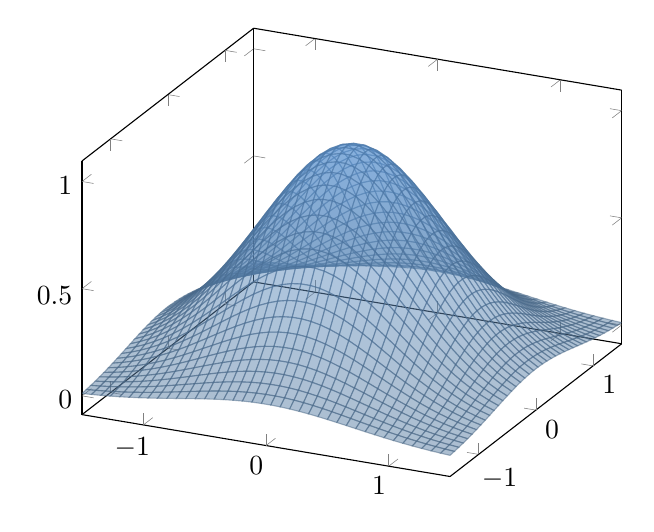
\begin{tikzpicture}
      \begin{axis}[domain=-1.5:1.5,y domain=-1.5:1.5, scale=1, colormap={custom}{color(0)=(DarkBlue3) color(1)=(BrightBlue1)}]
        \addplot3[draw=black, opacity=0.5, surf, samples=40] {exp(-x^2-y^2)};
      \end{axis}
    \end{tikzpicture}
   \captionsetup{labelformat=empty}
   \caption{Graphe de la fonction \(f : (x, y) \mapsto \exp(-x^2 - y^2)\)}
\end{figure}
On définit de meme \textbf{l'espace affine tangent} à la courbe de \(f\) au point \((a_1, \ldots, a_n)\) par:
\[
   \tau_{(a_1, \ldots, a_n)} := \Bigl\{ (x_1, \ldots, x_n, z) \in \R^{n+1} \; ; \; z = df_a(x_1 - a_1, \ldots, x_n - a_n) + f(a_1, \ldots, a_n) \Bigl\}    
\]

\subsection*{\subsecstyle{Gradient{:}}}
On va maintenant définir un autre opérateur différentiel sur l'ensemble des fonctions de classe \(\mathcal{C}^1(\R^n, \R)\), attention, ici il s'agit bien du cas particulier des champs de scalaires. On définit alors \textbf{l'opérateur gradient}:
\[
   \begin{aligned}
      \nabla : \mathcal{C}^1(\R^n, \R) &\longrightarrow \mathcal{L}(\R^n, \R^n)\\
      f &\longmapsto \nabla f = \left(\partialD{f}{x_1}, \ldots, \partialD{f}{x_n}\right)
   \end{aligned}
\]
Le gradient de \(f\) est donc un \textbf{champ de vecteurs}, dont on verra une interprétation ci-dessous, mais tout d'abord, on peut remarquer l'identité suivante en un point \(a\), qui le lie avec la différentielle:
\[
   \forall h \in \R^n \; ; \; \dotproduct{\nabla f(a)}{h} = \dotproduct{\left(\partialD{f}{x_1}(a), \ldots, \partialD{f}{x_n}(a)\right)}{h} = df_a(h)
\]

On cherche maintenant à interpréter ce que représente le gradient par rapport au champs scalaire \(f\), et on peut alors montrer la propriété géométrique suivante:
\begin{center}
   \textit{Le gradient est le champ de vecteurs qui donne la direction de la plus grand pente ascendante à la surface de la courbe de \(f\).}
\end{center}
\begin{figure}[h]
   \centering
   \vspace*{-0.5mm}
   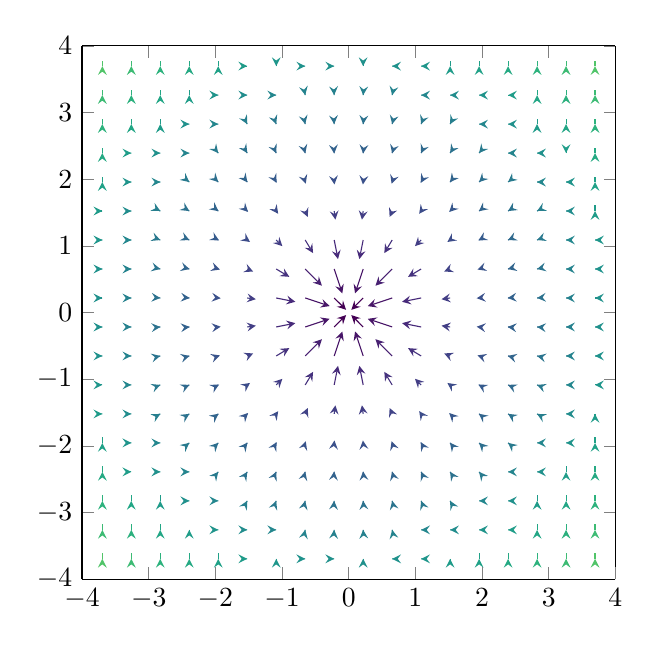
\begin{tikzpicture}
      \begin{axis}[%
         xmin = -4, xmax = 4,
         ymin = -4, ymax = 4,
         zmin = 0, zmax = 1,
         axis equal image,
         xtick distance = 1,
         ytick distance = 1,
         view = {0}{90},
         scale = 1.25,
         height=7cm,
         colormap/viridis,
      ]
      \addplot3[point meta = {sqrt(x^2+y^2)}, quiver={u=-2*x*exp(-x^2-y^2), v=-2*y*exp(-x^2-y^2), scale arrows=0.45}, quiver/colored = {mapped color}, samples=24, -stealth] (x,y,0);
     \end{axis}
   \end{tikzpicture}
   \captionsetup{labelformat=empty}
   \caption{Gradient de la fonction \(f : (x, y) \mapsto \exp(-x^2 - y^2)\)}
\end{figure}
Une autre propriété remarquable du gradient est qu'il est toujours \textbf{orthogonal} aux lignes de niveaux.

\subsection*{\subsecstyle{Caractérisation des dérivées directionnelles{:}}}
Pour un vecteur unitaire \(v\) donné, on peut alors montrer la caractérisation trés utile de la dérivée directionelle de \(f\) dans la direction de \(v\), en effet on a:
\[
   D_vf(a) = df_a(v) = \dotproduct{\nabla f(a)}{v}  
\]
En effet, il suffit alors d'écrire la formule de Taylor à l'ordre 1 sur la quantité ci-dessous et utiliser les différentes propriétés des objets considérés:
\[
   f(a + hv) - f(a) = df_a(hv) + o(\vectNorm{hv})
\]
\uline{Exemple:} Pour \(f(x,y) = xy + x\) et  \(v = \frac{1}{\sqrt{2}}(1, 1)\) alors on a:
\[
   df_{(x, y)} = (y+1)dx + xdy   
\]
Et donc finalement:
\[
   D_vf(x, y) = \frac{1}{\sqrt{2}}(y + x + 1)
\]
On peut remarque que si on prends \(v = e_i\), on retombe évidemment sur les dérivées partielles.
\pagebreak

\subsection*{\subsecstyle{Jacobienne{:}}}
On considère maintenant plus généralement l'espace des fonctions de classe \(\mathcal{C}^1(\R^n, \R^p)\), et on définit alors l'opérateur suivant:
\[
   \begin{aligned}
      J : \mathcal{C}^1(\R^n, \R^p) &\longrightarrow \mathcal{M}_{p, n}(\mathcal{F}(\R^n, \R^p))\\
      f &\longmapsto \begin{pmatrix}
         \partialD{f_1}{x_1} &\ldots &\partialD{f_1}{x_n}\\
         \vdots &\ddots &\vdots \\ 
         \partialD{f_p}{x_1} &\ldots &\partialD{f_p}{x_n}
      \end{pmatrix}
   \end{aligned}
\]
On appellera alors \textbf{jacobienne} de \(f\) la matrice \(Jf\), et on remarque que c'est simplement la matrice\footnote[1]{A coefficients dans l'anneau des fonctions.} constituée des dérivées partielles de \(f\).\<

En particulier, on a donc l'identité suivante:
\[
   Jf = \begin{pmatrix}
      \nabla f_1\\
      \vdots\\ 
      \nabla f_n
   \end{pmatrix}
\]
\begin{center}
   \textit{C'est aussi la matrice des gradients des applications partielles de \(f\).}
\end{center}
Si on l'évalue maintenant en un point \(a \in \R^n\), on obtient alors une matrice réelle et on a la caractérisation fondamentale suivante:
\begin{center}
   \textbf{La jacobienne prise en un point est la matrice de la différentielle en ce point.}
\end{center}
En particulier on retrouve donc la règle de la composition de la différentielle vu sous l'angle matriciel:
\[
   J(f \circ g)_a = Jf_{g(a)} \times Jg_{g(a)}
\]
Ainsi que la règle de l'inversion d'une fonction inversible:
\[
   (Jf_{a})^{-1} = J(f^{-1})_{f(a)}
\]

\chapter*{\chapterstyle{VII --- Etude d'Extrema}}
\addcontentsline{toc}{section}{Etude d'Extrema} 
Un des intérets de la notion de dérivée d'une fonction réelle est de pouvoir étudier les extrema de cette fonction, en particulier, un point capital du cours d'analyse réelle est la définition de \textbf{point critique}, qui sont les points d'annulation de la dérivée, et on a alors la condition nécessaire suivante:
\begin{center}
   \textbf{Si un point est un extremum, alors c'est un point critique.}
\end{center}
On veut généraliser cette notion au cas des \textbf{champs scalaires}

\subsection*{\subsecstyle{Points critiques{:}}}
De manière parfaitement analogue, si \(f\) est une fonction définie sur un ouvert \(\mathcal{U}\), alors on définit les \textbf{points critiques}, qui sont les points d'annulation de la différentielle, et on a alors la condition nécessaire suivante:
\begin{center}
   \textbf{Si un point est un extremum, alors c'est un point critique.}
\end{center}
Informellement, on comprends naturellement que les seuls extrema possibles seront ceux où l'application linéaire tangente est nulle, donc un plan horizontal. Néanmoins la condition n'est que nécessaire, en effet on considère la fonction:
\[
   f : (x, y) \mapsto xy   
\]
Alors sa différentielle est nulle en \((0, 0)\), mais ce point n'est pas un extremum, il suffit d'étudier quelques restrictions pour le montrer. On a donc besoin d'outils plus puissants pour trouver ces extrema. 

\subsection*{\subsecstyle{Hessienne{:}}}
On suppose maintenant que \(f \in \mathcal{C}^2(\R^n)\), alors elle admet toutes ses dérivées partielles secondes et elle vérifie le \textbf{théorème de Schwarz}. On définit alors la \textbf{matrice Hessienne} de \(f\) par:
\[
   \mathcal{H}f_{(x, y)} = \left(\partialD{{}^2f}{x_ix_j}\right)_{i ,j \in \inticc{1}{n}} = 
   \begin{pmatrix}
      \partialD{{}^2f}{x_1^2} & \ldots & \partialD{{}^2f}{x_1x_{n}}\\ 
      \vdots & \ddots & \vdots\\ 
      \partialD{{}^2f}{x_{1}x_n} & \ldots & \partialD{{}^2f}{x_{n}^2}\\   
   \end{pmatrix}   
\]
Cette matrice est \textbf{symétrique} d'aprés le théorème de Schwarz, elle définit donc une forme bilinéaire symétrique et une forme quadratique, qu'on appelera forme hessienne, qui jouera un rôle important pour la suite.
\subsection*{\subsecstyle{Classification des points critiques{:}}}
Dans le cas réel, pour classifier les points critiques d'une fonction, on étudiait la convexité de cette fonction, et en particulier le signe de la dérivée seconde, ceci permettait de différencier les maxima, minima et point cols (ou point d'inflexions). D'une certaine manière, on généralise cette approche au cas général en étudiant \textbf{le signe de la Hessienne} au sens du signe d'une forme quadratique, et on a les cas suivants:
\begin{itemize}
   \item Si la forme hessienne n'est \textbf{ni positive ni négative} en un point critique, alors le point est un \textbf{point col}.

   \item Si la forme hessienne est \textbf{définie positive} en un point critique, alors la fonction est localement convexe et le point est un \textbf{minimum}.
   \item Si la forme hessienne est \textbf{définie négative} en un point critique, alors la fonction est localement concave et le point est un \textbf{maximum}.
   \item Sinon la méthode ne permet pas de conclure.
\end{itemize}
On se ramène donc à l'étude des valeurs propres de la Hessienne, et de leurs signes ou dit autrement, de la signature de la forme quadratique Hessienne.

\chapter*{\chapterstyle{VII --- Théorèmes généraux}}
\addcontentsline{toc}{section}{Théorèmes généraux} 
Dans cette section, nous allons utiliser toutes les notions construites au chapitre précédent pour essayer de généraliser les grands théorèmes sur les fonctions réelles dérivables, en particulier les deux théorèmes suivants:
\begin{itemize}
   \item Le théorème de la bijection
   \item Le théorèmes des accroissements finis
\end{itemize}
Le problème principal pour obtenir un analogue au premier théorème est le suivant:
\begin{center}
   \textit{Il existe des fonctions non-injectives telles qu'en tout point leur différentielle soit inversible !}
\end{center}
Ce qui implique alors que nous ne pouvons pas prouver l'injectivité \textbf{globale} d'une fonctions à plusieurs variables avec le critère simple de la non-annulation de la différentielle. Ceci nous menera donc à la recherche de théorème permettant de montrer la bijectivité de ces fonctions autrement.

\subsection*{\subsecstyle{Théorème d'inversion locale{:}}}
On considère \(f : \R^n \longrightarrow \R^p\) de classe \(\mathcal{C}^1\) et un point \(a \in \R^n\), alors si sa différentielle est \textbf{inversible} en \(a\), on a:
\begin{center}
   \textbf{La fonction induit un \(\mathcal{C}^1\)-difféomorphisme d'un voisinage \(V_a\) dans \(f(V_a)\).}
\end{center}
On peut interpréter ce théorème de manière plus naturelle sous la forme:
\begin{center}
   \textit{Si la différentielle ne s'annule pas en un point, alors la fonction est localement inversible en ce point.}
\end{center}

\subsection*{\subsecstyle{Théorème d'inversion globale{:}}}
On considère \(f : \R^n \longrightarrow \R^p\) une fonction \textbf{injective} et de classe \(\mathcal{C}^1\), alors si en tout point d'un ouvert \(\mathcal{U}\) sa différentielle est \textbf{inversible}, on a:
\begin{center}
   \textbf{La fonction induit un \(\mathcal{C}^1\)-difféomorphisme de \(\mathcal{U}\) sur \(f(\mathcal{U}).\)}
\end{center}
On peut interpréter ce théorème de manière plus naturelle sous la forme:
\begin{center}
   \textit{Sous réserve d'injectivité, si la différentielle ne s'annule pas sur un ouvert, alors la fonction est inversible sur cet ouvert.}
\end{center}

\subsection*{\subsecstyle{Théorème des fonctions implicites{:}}}
On considère une fonctions \(f : \R^n \rightarrow \R\) de classe \(\mathcal{C}^1(\R^n)\) et on s'intéresse aux courbes \(\Gamma\) d'équation:
\[
   f(x_1, \ldots, x_n) = 0   
\]
Si il est possible d'exprimer une variable en fonction des autres, ie d'isoler une variable \(x_i\), alors on dira que l'équation \(E\) définit \(x_i\) comme \textbf{une fonction implicite} des \(n-1\) autres variables. On s'intéresse ici à des condition suffisantes sur \(f\) pour que de telles fonctions implicites existent.\<

On peut alors montrer gràce au \textbf{théorème d'inversion locale} que si \((x_1, \ldots, x_n) \in \Gamma\), et que la \(i\)-ème dérivée partielle ne s'annule pas, alors \textbf{localement} l'équation définit bien \(x_i\) comme fonction implicite des \(n-1\) autres variables pour un certaine fonction \(\phi\) de classe \(\mathcal{C}^1(\R^{n-1})\), ie on a:
\[
   x_i = \phi(x_1, \ldots, x_{i-1}, x_{i+1}, \ldots, x_n)   
\]
Prenons un exemple simple pour illustrer le propos
\pagebreak

On considère la courbe \(\Gamma\) suivante:
\[
   f(x,y) = x^2 + y^2 - 1 =0
\]
On reconnaît immédiatement le cercle unité, le théorème des fonctions implicites affirme alors qu'à l'exception des points \((\pm 1, 0)\), cette équation définit implicitement \(y\) comme une fonction de \(x\) et en effet, on sait que par exemple dans le demi-plan supérieur, on a:
\[
   y = \sqrt{1 - x^2}   
\]
Ce théorème justifie une technique courante dans la littérature anglo-saxonne nommé \textbf{différentiation implicite}, en effet si on considère une équation d'un fonction à deux variables (par exemple), alors on peut "voir"\footnote[1]{Sous les hypothèses de régularité du théorème bien évidemment.} une des variables comme fonction de l'autre et simplement différentier, et par exemple on peut de cette manière trouver les dérivées des fonctions réciproques:
\begin{flalign*}
   y = \cos^{-1}(x) &\Longleftrightarrow \cos(y) = x\\
   &\Longleftrightarrow \sin(y)y' = -1  \shorteqnote{(On "voit" \(y\) comme fonction de \(x\) et on différentie.)}\\
   &\Longleftrightarrow y' = \frac{-1}{\sin(y)}\\
   &\Longleftrightarrow y' = \frac{-1}{\sin(\cos^{-1}(x))}\\
   &\Longleftrightarrow y' = \frac{1}{-\sqrt{1-x^2}}
\end{flalign*}

\subsection*{\subsecstyle{Théorème des accroissements finis{:}}}
On considère ici un champs scalaire\footnote[2]{Il n'existe pas d'équivalent au théorème des accroissements finis dans le cas de fonctions à valeurs vectorielles, considérer par exemple la courbe \(t \mapsto (\cos(t), \sin(t))\).} défini et différentiable sur un ouvert \(\mathcal{U}\), alors pour tout point \(a, b \in \mathcal{U}\) tel que le segment \([a, b]\) les reliant soit dans \(\mathcal{U}\), on a\footnote[3]{La démonstration de cette propriété revient à se ramener au cas réel en posant \(g(t) = f((1 - t)a + tb)\)}:
\[
   \exists c \in \mathcal{U} \; ; \; f(b) - f(a) = df_c(b - a)   
\]
En particulier si \(\mathcal{U}\) est convexe, cette propriété est vrai pour tout couple \((a, b)\).

\subsection*{\subsecstyle{Corollaire 1 : Inégalité des accroissements finis{:}}}
En particulier, si la différentielle \(df_x\) est \textbf{bornée} par un réel \(M\) sur \(\mathcal{U}\), alors on a aussi:
\[
   |f(b) - f(a)| \leq M(b - a)
\]
Cette majoration reste vraie, contrairement au théorème, dans le cas de champs de vecteurs et on a alors pour des normes bien choisies:
\[
   \vectNorm{f(b) - f(a)} \leq M\vectNorm{b - a}
\]
En particulier, cela montre donc que les applications différentiables sont toutes \textbf{localement} lipschitziennes, et même globablement lipschitziennes si la différentielle est bornée.

\subsection*{\subsecstyle{Corollaire 2 : Applications constantes {:}}}
On peut alors généraliser le critère des fonctions réelles qui nous affirme que si la dérivée d'une fonction est nulle, elle est constante. En effet, si \(f : \mathcal{U} \rightarrow \R\) différentiable sur \(\mathcal{U}\) ouvert et \textbf{connexe}\footnote[4]{La preuve est directe si \(\mathcal{U}\) est convexe, pour passer à la connexité, il faut alors remarque que toutes les boules sont convexes.}, alors:
\begin{center}
   Si la différentielle de \(f\) est \textbf{nulle} sur \(\mathcal{U}\), alors \(f\) est \textbf{constante} sur \(\mathcal{U}\).
\end{center}

\subsection*{\subsecstyle{Corollaire 3 : Applications constantes par rapport à une variable {:}}}
On s'intéresse alors à ce qu'on peut déduire de l'annulation d'une seule des dérivées partielles, et en se ramenant à l'étude des application partielles on peut alors montrer que si \(f : \mathcal{U} \rightarrow \R\) différentiable sur \(\mathcal{U}\) ouvert et \textbf{convexe}\footnote[2]{\textbf{ATTENTION:} Ce résultat est faux sur un domaine juste connexe. Prendre la fonction qui définie sur \(\R^2\) privée d'un axe bien choisi qui vaut \(0\) sur \(\{ (x, y), xy < 0\}\) et \(x^2\) ailleurs.} et que \(\partialD{f}{x_i}\) est \textbf{nulle} sur \(\mathcal{U}\), alors il existe une fonction \(g\) telle que:
\[
   \forall (x_1, \ldots, x_n) \in \mathcal{U} \; f(x_1, \ldots, x_n) = g(x_1, \ldots, x_{i-1}, x_{i+1}, \ldots, x_n) 
\]
\begin{center}
   \textit{Intuitivement, on l'interprète simplement par le fait que \(f\) ne dépends pas de la variable \(x_i\) sur cet ouvert.}
\end{center}
C'est ce corollaire qui nous permettra de résoudre nos premières équations aux dérivées partielles. Voici un exemple élementaire, on considère une fonction \(f\) de classe \(\mathcal{C}^1(\R^2)\) qui vérifie:
\[
   \partialD{f}{x}(x, y) = 0   
\]
Alors d'aprés ce corollaire, on a directement, pour \(g \in \mathcal{C}^1(\R)\) une certaine fonction réelle:
\[
   f(x, y) = g(y)   
\]

\chapter*{\chapterstyle{VII --- Formes différentielles}}


\chapter*{\chapterstyle{VII --- Intégrales Curvilignes}}
\addcontentsline{toc}{section}{Intégrales Curvilignes} 

Dans cette partie, nous allons généraliser l'intégrale de Riemann, c'est à dire l'intégrale d'une fonction le long d'un segment, aux \textbf{champs scalaires et vectoriels}, avec en tête l'idée suivante:
\begin{center}
   \textit{On veut pouvoir intégrer un champ le long d'une courbe lisse donnée.}
\end{center}
Nous verrons alors qu'il existe en fait trois constructions différentes qui mesurent différents phénomênes sur les champs considérés:
\begin{itemize}
   \item L'intégrale d'un \textbf{champ scalaire} qui quantifie l'aire entre la courbe et le plan des paramétres.
   \item L'intégrale de \textbf{travail} d'un \textbf{champ vectoriel} qui quantifie la contribution du champ vectoriel au trajet de la courbe.
   \item L'intégrale de \textbf{flux} d'un \textbf{champ vectoriel} qui quantifie la tendance au champ de vecteurs à traverser la courbe.
\end{itemize}
Dans toute la suite, on considèrera un \textbf{arc orienté} \(\Gamma\) paramétré par une fonction \(\gamma : t \mapsto \gamma(t)\) définie sur \(\icc{a}{b}\) et de classe \(\mathcal{C}^1\). On rapelle à toutes fins utiles:
\begin{itemize}
   \item L'abcisse curviligne de \(\gamma\) est donnée par: \(ds = \vectNorm{\gamma'(t)} \d t  \)
   \item Le vecteur normal à \(\gamma'\) est donnée par: \(dn = (\gamma_2'(t), -\gamma_1'(t))\d t  \)
\end{itemize}
\subsection*{\subsecstyle{Intégrale d'un champ scalaire{:}}}
On se donne un champ scalaire lisse \(f : \Gamma \rightarrow \R\) et on cherche à quantifier l'aire située entre la courbe et le graphe \(\mathscr{G}_f\), on peut alors écrire cette aire comme une somme de Riemann, qui tends alors vers une intégrale et on définit:
\[
   \int_{\gamma} f \d s = \int_{a}^{b}f(\gamma(t))\vectNorm{\gamma'(t)}\d t
\]
\subsection*{\subsecstyle{Intégrale de travail d'un champ vectoriel{:}}}
On se donne un champ vectoriel lisse \(f : \Gamma \rightarrow \R^n\) et on cherche à quantifier la \textbf{contribution du champ vectoriel au trajet de la courbe}, ie au travail que le champ effectuerais sur une particule qui se déplacerait le long de la courbe, à nouveau gràce aux sommes de Riemann, on peut définir:
\[
   \int_{\gamma} F \d \gamma = \int_{a}^{b} \dotproduct{F(\gamma(t))}{\gamma'(t)}\d t
\]
\subsection*{\subsecstyle{Intégrale de flux d'un champ vectoriel{:}}}
On se donne un champ vectoriel lisse \(f : \Gamma \rightarrow \R^n\) et on cherche à quantifier la \textbf{tendance au champ de vecteurs à traverser la courbe}, ie si le champ de vecteurs représenterais un fluide, à la quantité d'eau qui traverse la courbe en un instant donné. A nouveau gràce aux sommes de Riemann, on peut définir:
\[
   \int_{\gamma} F \d n = \int_{a}^{b} \dotproduct{F(\gamma(t))}{n'(t)}\d t
\]
\subsection*{\subsecstyle{Intprétation du produit scalaire{:}}}
On remarque que les intégrales curviligne d'un champ de vecteur font apparaître un produit scalaire, en effet cela déocule directement des quantités géométriques que l'on cherche à calculer:
\begin{itemize}
   \item Dans le cas d'une intégrale de travail, on considère la projection d'un vecteur du champ sur un vecteur tangent, c'est \textbf{la composante tangentielle} du champ, et on somme toutes ses composantes pour obtenir une contribution totale.
   \item Dans le cas d'une intégrale de flux, on considère la projection d'un vecteur du champ sur un vecteur normal, c'est \textbf{la composante normale} du champ, et on somme toutes ses composantes pour obtenir une contribution totale mais dans un autre sens.
\end{itemize}
\subsection*{\subsecstyle{Théorème du gradient{:}}}
On s'attarde un peu sur le cas vectoriel, et on se donne un champ vectoriel \(X\) tel que \(X = \nabla F\) pour un certain champ scalaire \(F\), on dira alors que \(X\) \textbf{dérive du potentiel} \(F\), on se donne un chemin paramétré par \(\gamma\) sur \(\icc{a}{b}\) et on cherche à calculer le travail de \(X\) sur ce chemin, on trouve alors que:
\begin{flalign*}
   \int_{\gamma} X \d \gamma &:= \int_{a}^{b} \dotproduct{\nabla F(\gamma(t))}{\gamma'(t)}\d t \\
   &= \int_{a}^{b} dF_{\gamma(t)}(\gamma'(t)) \d t \shorteqnote{(On utilise le lien gradient / différentielle.)} \\ 
   &= \int_{a}^{b} d(F \circ \gamma)_t \shorteqnote{(Par la règle de la chaîne, ou en passant en composantes.)}  \\ 
   &= \int_{a}^{b} (F \circ \gamma)'(t) \d t \shorteqnote{(Par le lien diférentielle / dérivée.)}  \\ 
   &= F(\gamma(b)) - F(\gamma(a)) \shorteqnote{(Théorème fondamental de l'analyse.)}  \\ 
\end{flalign*}
En particulier, on a montré le théorème suivant, généralisation du théorème fondamental de l'analyse, appelé souvent \textbf{théorème du gradient}:
\begin{center}
   \textbf{Le travail le long d'un chemin d'un champ qui dérive d'un potentiel ne dépends que des bords du chemin choisi.}
\end{center}
C'est en fait même un cas particulier d'un théorème trés général qu'on verra plus tard apellé \textbf{théorème de Stokes} qui affirme que pour une forme différentielle \textbf{exacte}, ie qui s'écrive \(\d\omega\) pour \(\omega\) une autre forme différentielle, alors on a que l'intégrale ne dépends que des bords:
\[
   \int_{A} \d \omega = \int_{\partial A} \omega
\]
\subsection*{\subsecstyle{Généralisations{:}}}
On imagine alors qu'il doit être possible de généraliser ces concepts d'intégrales sur une courbe (espace de dimension 1) à des intégrales sur des \textbf{surfaces, volumes ...}. On aurait alors les deux\footnote[1]{Le concept d'intégrale de travail ne se généralise pas conceptuellement aux dimensions plus grandes pour des raisons évidentes.} concepts géométriques suivants:
\begin{itemize}
   \item L'intégrale sur une surface d'un \textbf{champ scalaire} qui quantifierait le volume entre la courbe et le plan des paramétres.
   \item L'intégrale sur une surface d'un \textbf{champ vectoriel} qui quantifierait la tendance au champ de vecteurs à traverser la surface.
\end{itemize}

\chapter*{\chapterstyle{VII --- Intégrales Multiples}}
\addcontentsline{toc}{section}{Intégrales Curvilignes} 
Dans ce chapitre on cherche à généraliser la notion d'intégrale d'une fonction d'une seule variable sur un segment à la notion d'intégrale d'une fonction réelle \textbf{de plusieurs variables qu'on supposera bornée}, ici on considérera principalement \(f : \R^2 \rightarrow \R\) pour simplifier l'exposition. On a alors deux nouveaux concepts d'intégrales qui se présentent:
\begin{itemize}
   \item La notion d'intégrale \textbf{curviligne} qui se propose d'intégrer à nouveau sur un chemin (donc toujours sur un espace de dimension 1).
   \item La notion d'intégrale \textbf{multiple} qui se propose d'intégrer sur une surface (donc sur un espace de dimension plus grande).
\end{itemize}
Ces deux notions différentes coexistent et permettent de résoudre des problèmes trés différents, nous nous proposons ici tout d'abord de définir la notion d'intégrale multiple. Moralement, l'idée consiste à se donner un domaine raisonnable \(\mathcal{D}\) de \(\R^2\), et de chercher à calculer le \textbf{volume} au dessus \(\mathcal{D}\) et contenu sous la nappe définie par l'image de \(f\). 

Graphiquement, voila ce que l'on cherche à réaliser, ici le domaine d'intégration étant un simple rectangle:
\begin{center}
   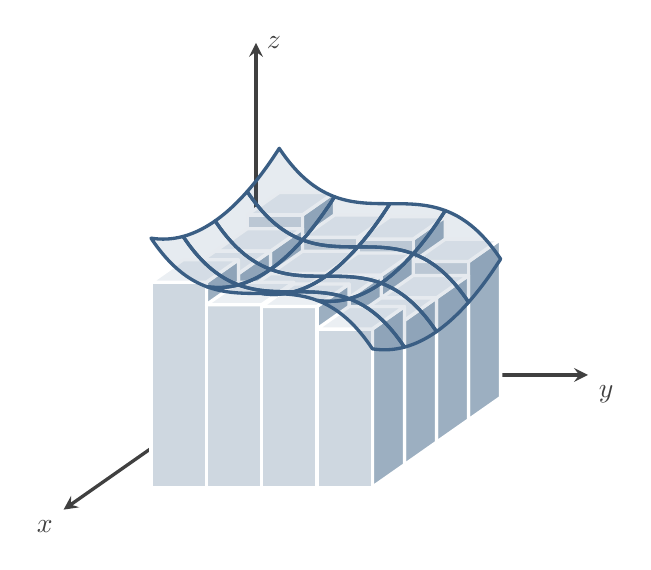
\begin{tikzpicture}[
      x=(215:2em/sqrt 2), y=(0:2em), z=(90:2em),
      declare function={f(\x,\y)=((\x-3)^2+(-\y+3)^3)/8+3;}, 
      very thick, line join=round]
    \draw [-stealth, black!75] (0,0,0) -- (6,0,0) node [below left] {$x$};
    \draw [-stealth, black!75] (0,0,0) -- (0,6,0) node [below right] {$y$};
    \draw [-stealth, black!75] (0,0,0) -- (0,0,6) node [right] {$z$};
    \foreach \x in {1,...,4}
      \foreach \y [evaluate={\j=\x+.5; \i=\y+.5; \k=f(\j,\i);}] in {1,...,4}{
        \path [fill=DarkBlue2!50, draw=white] (\x, \y+1, 0) -- (\x+1, \y+1, 0) -- 
          (\x+1, \y+1, \k) -- (\x, \y+1, \k) -- cycle;
        \path [fill=DarkBlue2!25, draw=white] (\x+1, \y, 0) -- (\x+1, \y+1, 0) -- 
          (\x+1, \y+1, \k) -- (\x+1, \y, \k) -- cycle;
        \path [fill=DarkBlue2!10, draw=white] (\x, \y, \k)  -- (\x+1, \y, \k) -- 
          (\x+1, \y+1, \k) -- (\x, \y+1, \k) -- cycle;
      }
     \foreach \x in {1,...,4}
       \foreach \y in {1,...,4}{
     \draw [DarkBlue2, fill=DarkBlue2, fill opacity=0.125, 
        domain=0:1, samples=20, variable=\t] 
        plot (\x+\t, \y, {f(\x+\t,\y)}) -- 
        plot (\x+1, \y+\t, {f(\x+1,\y+\t)}) -- 
        plot (\x+1-\t, \y+1, {f(\x+1-\t,\y+1)}) --
        plot (\x, \y+1-\t, {f(\x,\y+1-\t)}) -- cycle;
      }


    \end{tikzpicture}
\end{center}

\subsection*{\subsecstyle{Outils préliminaires{:}}}
On souhaite intégrer \(f\) sur le rectangle \(R = [a, b] \times [c, d]\), on considère alors une \textbf{subdivision} de \(R\) c'est à dire un couple de subdivisions de \([a, b] \text{ et } [c, d]\) respectivement, ie on se donne \((a = t_0, t_1, \ldots, t_{n-1}, t_n = b)\) et \((c = t'_0, t'_1, \ldots, t'_{n-1}, t'_n = d)\), alors ces subdivisions définissent des \textbf{sous-rectangles} par:
\[
   R_ij = [t_i, t_{i+1}] \times [t'_j, t'_{j+1}]   
\]
On appellera la collection de ces sous-rectangles une \textbf{subdivision} du rectangle \(R\). On définit de manière évidente le \textbf{volume} (ici une aire) d'un rectangle \(R\) par:
\[
   \text{Vol}(R) = (b - a)(d - c) 
\]
Finalement on définit aussi les deux quantités suivantes pour tout rectangle \(R\):
\[
   \begin{cases}
      m_R(f) &:= \left\{ \inf(f(x)) \, ; \, x \in R \right\}\\
      M_R(f) &:= \left\{ \sup(f(x)) \, ; \, x \in R \right\}
   \end{cases}   
\]
\pagebreak
\subsection*{\subsecstyle{Intégrale sur un rectangle{:}}}
Soit \(R\) le rectangle domaine d'intégration et \(P\) une subdivision de \(R\), alors on définit les \textbf{sommes de Darboux supérieure et inférieures} par:
\[
   \begin{cases}
      S_P^+(f) = \sum_R M_R(f) \cdot \text{Vol}(R)\\
      S_P^-(f) = \sum_R m_R(f) \cdot \text{Vol}(R) 
   \end{cases}
\] 
Où la somme parcourt tout les rectangles de la subdivision. On définit alors les \textbf{intégrales de Darboux supérieure et inférieures} par:
\[
   \begin{cases}
      \displaystyle\int_R^+{f} = \inf\left\{\, S_P^+(f)\; ; \; P \text{ est une subdivision de } R\right\}\\
      \displaystyle\int_R^-{f} = \sup\left\{\, S_P^-(f)\; ; \; P \text{ est une subdivision de } R\right\}
   \end{cases}
\]
\begin{center}
   \textit{
      L'intégrale supérieure (resp. inférieure) est la somme \textbf{minimale} (resp. maximale) obtenue en considérant \textbf{toutes les subdivisions possibles} du rectangle.
   }
\end{center}
Enfin on dit que \(f\) est \textbf{intégrable} sur \(R\) si et seulement si \textbf{l'intégrale supérieure et inférieure} sont égales, et on la note formellement:
\[
   \int_R f \d x_1 \ldots \d x_n \overset{\text{def.}}{=} \int_R f 
\]


\subsection*{\subsecstyle{Intégrale sur un ensemble borné{:}}}


.... -> Admettons pour le moment que l'on sait intégrer sur des surfaces ...

   \pagebreak   
   
   \addcontentsline{toc}{chapter}{Analyse Complexe} % A FAIRE
   \chapter*{\chapterstyle{VIII --- Introduction}} % A REFAIRE
\addcontentsline{toc}{section}{Introduction} 
Dans ce chapitre nous étudirons les propriétés des fonctions définies sur l'ensemble des complexes. En particulier nous chercherons à définir une notion de \textbf{différentielle} puis une notion \textbf{d'intégrale} pour ces fonctions et enfin étudier les propriétés des ces deux constructions.\+

On rapelle à tout fins utiles \(\C\) est défini par la structure \((\R^2, +, \times)\) avec une multiplication définie par:
\[
   (a, b)(c, d) = (ac - bd, ad + bc)
\]
On rapelle aussi que l'on a \(\C \cong \R^2\) et en particulier la représentation des nombres complexes en tant que couple nous donne une représentation de la multiplication complexe par le produit matriciel suivant:
\[
   (a + bi)(c + di) = ac - bd + i(ad + bc) \sim (ac - bd, ad + bc) =  \begin{pmatrix}
      a & -b \\
      b & a
   \end{pmatrix} \begin{pmatrix}  c \\ d \end{pmatrix}
\]
\subsection*{\subsecstyle{Applications conformes {:}}}
On appelle \textbf{application conforme} toute application qui préservent les angles. En particulier, si on se donne \(\Gamma\) une courbe paramétrée par \(\gamma\) sur \(I\), et \(f\) un application, alors on dira:

est conforme si et seulement si


\chapter*{\chapterstyle{VIII --- Fonctions Holomorphes}} % A REFAIRE
\addcontentsline{toc}{section}{Fonctions Holomorphes} 
On définit ici la notion de \textbf{différentielle complexe}, qui sera une généralisation directe de la différentielle dans le cas réel, en effet on dira que \(f\) est \textbf{différentiable} en \(a\) si et seulement si le taux d'accroissement suivant, appelée dérivée de \(f\) en \(a\) existe:
\[
   \lim_{z \rightarrow a} \frac{f(z) - f(a)}{z - a} = f'(a)
\]
Où de manière équivalente si il existe une application \(\C\)-linéaire \(L\) telle que dans un voisinage de \(a\) on ait:
\[
   f(z) - f(a) - L(z - a) = o(z - a)
\]
On peut alors définir la différentielle de \(f\) en chaque point où elle existe par:
\[
   df : a \in \C \mapsto f'(a)dz
\]
On dira alors que \(f\) est holomorphe sur un ouvert si elle y est holomorphe en tout point, et qu'elle est \textbf{entière} si elle est holomorphe sur \(\C\).
\subsection*{\subsecstyle{Propriétés opératoires{:}}}
En particulier, vu que la définition de la différentielle est analogue à la différentielle réelle, on a alors (par les mêmes démonstrations) toutes les propriétés opératoires de l'opérateur de différentiation, en particulier:
\begin{itemize}
   \item La différentiation est un opérateur linéaire.
   \item La différentiation d'un produit suit la règle de Leibniz.
   \item La différentiation d'une composée suit la règle réelle de différentiation d'une composée.
   \item Le théorème d'inversion local nous donne la différentielle d'une réciproque.
\end{itemize}

\subsection*{\subsecstyle{Différences avec la différentiation réelle {:}}}
Ici on remarque tout de suite la différence notable qui est que la différentielle, qu'on sait être un champ de formes linéaires, est en fait un champ de forme \(\K\)-linéaires selon le corps dans lequel on différentie, ici on nécéssite que la forme soit \(\C\)-linéaire, ce qui va changer ses propriétés.\<

En particulier, on considère une fonction holomorphe \(f\) et on va calculer sa dérivée (directionelle) en \(z\) selon deux restrictions, une par valeurs \textbf{réelles uniquement}, l'autre par valeurs \textbf{imaginaires uniquement}, on obtient alors les deux taux d'accroissements suivants:
\[
   \lim_{h \underset{\R}{\rightarrow} 0} \frac{f(z + h) - f(z)}{h} \quad \quad \quad \lim_{h \underset{i\R}{\rightarrow} 0} \frac{f(z + h) - f(z)}{h}
\]
On sait qu'à tout fonction complexe, on peut associer une fonction sur \(\R^2\), et on va alors étudier les propriétés de ces taux d'accroissements en identifiant \(f(z) \sim f(x, y) = u(x, y) + iv(x, y)\), qui est bien différentiable au sens réel. En développant les taux d'accroissements ci-dessus en \((u, v)\), on obtient alors les deux égalités suivantes:
\[
   \begin{cases}
      f'(x, y) = \partialD{u}{x}(x, y) + i\partialD{v}{x}(x, y)\\
      f'(x, y) = \partialD{v}{y}(x, y) - i\partialD{u}{y}(x, y)
   \end{cases}
\]
Et enfin en regroupant ces égalités et en identifiant les parties réelles et imaginaires, on obtient alors que tout fonction holomorphe vérifie les \textbf{équations de Cauchy-Riemann}:
\[
   \begin{cases}
      \partialD{u}{x}(x, y) = \partialD{v}{y}(x, y)\\
      \partialD{v}{x}(x, y) = \partialD{u}{y}(x, y)
   \end{cases}
\]
\pagebreak 
\subsection*{\subsecstyle{Equations de Cauchy-Riemann{:}}}
En fait, on peut même montrer que ces équations caractérisent l'holomorphie, en effet pour \(f : \C \rightarrow \C\), on a:
\begin{center}
   \textbf{Si est différentiable \textbf{au sens réel} et vérifie les équations de Cauchy-Riemann, alors elle est holomorphe et réciproquement.}
\end{center}
\uline{Exemple:} Considérons la fonction \(f(z) = \overline{z}\), alors on a \(f(z) \sim f(x, y) = x - iy\) différentiable sur tout son domaine de définition mais on a:
\[
   \partialD{u}{x} = 1 \neq -1 = \partialD{v}{y} 
\]
Donc nécéssairement, la fonction conjugué n'est donc \textbf{pas holomorphe}.
\subsection*{\subsecstyle{Equations de Laplace{:}}}
On appelle \textbf{équations de Laplace} une équation aux dérivées partielles de la forme:
\[
   \partialD{{}^2f}{x_1^2} + \ldots + \partialD{{}^2f}{x_n^2} = 0
\]
Et on appelle alors \textbf{Laplacien} l'opérateur suivant:
\[
   \Delta = \partialD{{}^2}{x_1^2} + \ldots + \partialD{{}^2}{x_n^2}
\]
On appellera alors toute fonction solution des équations de Laplace \textbf{fonction harmonique}, et un des résultats intéressants de l'analyse complexe permet de montrer le résultat suivant:
\begin{center}
   \textbf{Toute fonction analytique telle que ses dérivées partielles secondes soient continues est harmonique.}
\end{center}


\chapter*{\chapterstyle{VIII --- Intégration Complexe}} % A REFAIRE
\addcontentsline{toc}{section}{Intégration Complexe} 
On cherche maintenant à définir une notion \textbf{d'intégrale} pour les fonctions complexe, plus précisément nous allons définir l'intégrale d'une fonction continue \(f\) le long d'une courbe paramétrée par \(\gamma\) sur \(\icc{a}{b}\), qui sera défini par l'intégrale suivante:
\[
   \int_{\gamma} f d\gamma = \int_{a}^{b} f(\gamma(t))\gamma'(t) d t
\]
L'intérprétation géométrique n'est pas évidente, mais peut s'éclaircir si on considère \(f(z) \sim f(x, y)\) et \(\overline{f}(z) = f(x, -y)\) le (champ vectoriel) conjugué de \(f\) apellé \textbf{champ de Pòlya}, alors on a pour des notations usuelles:
\[
   \int_{\gamma} f d\gamma = \int_{\gamma} \dotproduct{\overline{f}(\gamma(t))}{T(t)} d t + i \int_{\gamma} \dotproduct{\overline{f}(\gamma(t))}{N(t)}  d t
\]
En d'autres termes, cette intégrale encapsule \textbf{le travail et le flux du champ de Pòlya}.

\subsection*{\subsecstyle{Théorème fondamental de l'analyse complexe{:}}}
On se donne une fonction continue \(f\) tel que \(f =  F'\) pour une certaine fonction holomorphe \(F\) et on se donne un chemin paramétré par \(\gamma\) sur \(\icc{a}{b}\) et on cherche à calculer l'intégrale le long de ce chemin, alors on trouve:
\begin{align*}
   \int_{\gamma} f d \gamma &:= \int_{a}^{b} F'(\gamma(t))\gamma'(t)d t = \int_{a}^{b} (F \circ \gamma)'(t) d t = F(\gamma(b)) - F(\gamma(a))
\end{align*}
Ce n'est pas surprenant quand on comprends la dualité qui existe entre fonction complexe et champ vectoriel, ce n'est alors qu'un cas particulier du \textbf{théorème du gradient} vu en analyse vectorielle. Et aussi, comme énoncé dans le chapitre en question, c'est aussi un cas particulier du \textbf{théorème de Stokes} pour la forme différentielle exacte \(f(z)dz\).
\chapter*{\chapterstyle{VIII --- Quelques extensions}} % A REFAIRE
\addcontentsline{toc}{section}{Quelques extensions} 
\chapter*{\chapterstyle{VIII --- Grands Théorèmes}} % A REFAIRE
\addcontentsline{toc}{section}{Grands Théorèmes} 
   \pagebreak  

   \addcontentsline{toc}{chapter}{Equations Différentielles Ordinaires} % A FAIRE
   \chapter*{\chapterstyle{IX --- Introduction}}
\addcontentsline{toc}{section}{Introduction} 
Soit \(n, p\) des entiers et \(F\) une fonction \textbf{continue} sur \(\Omega \subseteq \R \times (\R^{p})^n\), alors on appelle \textbf{équation différentielle ordinaire} d'ordre \(n\) tout équation de la forme:
\[
   F(t, y(t), \ldots, y^{(n)}(t)) = 0
\]
Où \(y\) est une fonction d'un intervalle \( I \) dans \(\R^p\) à déterminer. Par exemple, on pose:
\[
   \begin{cases}
      F_1(t, y, y') = y'(t) - y(t)\\
      F_2(t, y, y') = cos(t)y'(t) - y^2(t)\\
      F_3(t, y, y') = 3 + arctan(t) + y'(t) - e^xy(t)\\ 
      F_4(t, y, y', y'') = t^2 + 3y(t)y'(t) + cos(y''(t))
   \end{cases} \implies
   \begin{cases}
      E_1 : y'(t) - y(t) = 0 \\
      E_2 : cos(t)y'(t) - y^2(t) = 0 \\
      E_3 : 3 + arctan(t) + y'(t) - e^xy(t) = 0 \\
      E_4 : t^2 + 3y(t)y'(t) + cos(y''(t)) = 0
   \end{cases}
\]
On peut aussi remarque que cette définition permet à \(y\) d'être à valeurs vectorielles et dans ce cas on obtient alors un \textbf{système différentiel}, par exemple pour \(E = \R^2\) et \(F_1\), on obtient:
\[
   E : \begin{cases}
      y'_1(t) = y_1(t)\\
      y'_2(t) = y_2(t)
   \end{cases}
\]
\subsection*{\subsecstyle{Forme résolue{:}}}
Dans des cas trés précieux, on peut isoler la plus grand dérivée, et on dira alors que l'équation différentielle est \textbf{sous forme résolue} si et seulement si il existe une fonction \(F\) continue sur \(\R \times (\R^p)^{n}\) telle que:
\[
   y^{(n)}(t) = F(t, y(t), \ldots, y^{(n-1)}(t))
\]
On ne s'intéressera dans ce cours qu'à ce cas particulier pour simplifier la compréhension, sauf cas simples où l'on peut se ramener à une forme réduite. Par la suite on appelera \textbf{équation associée à \( F \)} d'ordre \( n \) une équation de la forme ci-dessus.
\subsection*{\subsecstyle{Solution d'une équation différentielle{:}}}
On dira que \((I, y)\) est une \textbf{solution} de l'équation différentiellé d'ordre \( n \) associée à \( F \) si et seulement si \( I \) est un intervalle, \(y \in \mathcal{C}^n(I, \R^p)\) et que:
\[ 
   \forall t \in I \; ; \; (t, y(t), \ldots, y^{(n-1)}(t)) \in \Omega \; \text{ et } \; y^{(n)}(t) = F(t, y(t), \ldots, y^{(n-1)}(t))
\]
On remarque alors que le domaine de définition d'une même fonction solution peut changer et on peut alors définir une notion de solution \textbf{maximale et globale} par:
\begin{itemize}
   \item Une solution est \textbf{maximale} si et seulement si elle ne peut pas être prolongée en une autre solution définie sur une intervalle.
   \item Une solution est \textbf{globale} si et seulement \( \Omega \) est de la forme \(I \times (\R^p)^{n}\) et que \( y \) est une solution définie sur \( I \).
\end{itemize}
\subsection*{\subsecstyle{Réduction de l'ordre{:}}}
On se donne une équations différentielle résolue d'ordre \(n\), alors on pose:
\[
   Y(t) := \begin{pmatrix}
      y(t)\\
      y'(t)\\
      \vdots\\
      y^{(n-1)}(t)
   \end{pmatrix} \quad \quad \quad \quad\quad
   \mathbb{F}(t, Y(t)) := \begin{pmatrix}
      y'(t)\\
      y''(t)\\
      \vdots\\
      F(t, Y(t))
   \end{pmatrix}
\]
Alors on a directement que:
\[
   y^{(n)}(x) = F(x, y(x), \ldots, y^{(n-1)}(x)) \Longleftrightarrow Y'(x) = \mathbb{F}(x, Y(x))
\]
\begin{center}
   \textit{Fondamentalement, comprendre les EDO à l'ordre 1 c'est comprendre toutes les EDO.}
\end{center}
\subsection*{\subsecstyle{Problème de Cauchy{:}}}
Etant donné une équation d'ordre 1, et \( (t_0, y_0) \in \Omega \), on appele \textbf{problème de Cauchy} associée à l'équation \( (E) \) le problème suivant:
\[ 
   P: \begin{cases}
      y' = f(t, y)\\
      y(t_0) = y_0
   \end{cases} 
\]
Une question fondamentale de la théorie des equations differentielles ordinaires consiste à savoir sous quelles hypothèses sur \(  f \)tout problème de Cauchy associé à une équation admet une solution et les propriété de celles ci.
\subsection*{\subsecstyle{Raccordement de solutions{:}}}
Si on obtient deux solutions \( ( \ioo{a}{b}, y_1), (\ioo{b}{c}, y_2) \), alors on peut s'intéresser à raccorder ces deux solutions en une unique solution sur \( \ioo{a}{c} \). C'est en fait possible sous la condition suivante:
\[ 
   \lim_{x \rightarrow b} y_1(b) = \lim_{x \rightarrow b} y_2(b)
\]
\subsection*{\subsecstyle{Expression intégrale des solutions{:}}}
Considérons l'équation du premier ordre \((E)\) et le problème de Cauchy associé au couple \( (t_0, y_0) \), alors \( y \) est solution du problème de Cauchy ssi:
\[ 
   \forall t \in I \; ; \; y(t) = y_0 + \int_{t_0}^t f(s, y(s))ds 
\]
En réinterprétant cette équation et en définissant l'opérateur suivant:
\[ 
   \Phi : y \in \mathcal{C}^0(I, \R^p) \longmapsto (t \mapsto y_0 + \int_{t_0}^t f(s, y(s))ds) \in \mathcal{C}^0(I, \R^p)
\]
Alors une solution est exactement un \textbf{point fixe} de cet opérateur.

\subsection*{\subsecstyle{Equations à paramêtres{:}}}
On peut aussi pour tout paramêtre \( \lambda \in \Lambda \), où \( \Lambda \) est un espace vectoriel de dimension finie, définir une \textbf{équation différentielle à paramètre}, de la forme:
\[ 
   (E_\lambda) : y'(t) = f_\lambda(t, y(t)) 
\]
Résoudre une telle équation revient alors à résoudre une famille d'équations différentielles.
\chapter*{\chapterstyle{IX --- Théorie linéaire}}
\addcontentsline{toc}{section}{Théorie linéaire} 
On appele donc une équation différentielle linéaire une équation différentielle de la forme suivante:
\[ 
   y'(t) = A(t)y(t) + B(t) 
\]
Où \(A \in \mathcal{C}^0(I, \mathcal{M}_p( \K))\) et \(B \in \mathcal{C}^0(I, \mathcal{M}_{p, 1}( \K))\). Ce type d'équation trés spécifique permet d'utiliser la théorie de l'algèbre linéaire pour en trouver des solutions et/ou étudier leurs solutions.
\subsection*{\subsecstyle{Théorème de Cauchy-Lipschitz linéaire{:}}}
Alors gràce au théorème de Banach-Picard et à l'opérateur intégral défini plus haut, on peut montrer le résultat fondamental suivant, si on considère le problème de Cauchy linéaire suivant:
\[ 
   P: \begin{cases}
      y' = A(t)y(t) + B(t)\\
      y(t_0) = y_0
   \end{cases} 
\]
Alors on peut montrer le théorème dit de \textbf{Cauchy-Lipschitz linéaire}:
\begin{center}
   Ce problème admet une \textbf{unique solution} et elle est \textbf{globale}.
\end{center}
\subsection*{\subsecstyle{Exponentielle matricielle{:}}}
Dans le cas linéaire, on peut généraliser la résolution de l'équation élémentaire \( y'(t) = a(t)y(t) \) en étandant le domaine de définition de la fonction exponentielle, en effet pour tout matrice \( A \in \mathcal{M}_n(\K) \), on définit:
\[ 
   e^A = \sum_{n \in \N} \frac{A^n}{n!} 
\]
En effet, on munit \( \mathcal{M}_n(\K) \) d'une norme matricielle, et on peut alors montrer que cette série converge normalement, donc converge car \( \mathcal{M}_n(\K) \) est complet. On peut alors montrer les propriétés suivantes:
\begin{itemize}
   \item On a \( e^0 = 1\).
   \item On a \( e^A \) est inversible d'inverse \( e^{-A} \).
   \item On a \( e^{A+B} = e^Ae^B \) si \( A \) et \( B \) commutent.
\end{itemize}
Si on considère plus généralement une fonction matricielle \( A(t) \in \mathcal{C}^1\), et que \( A(t), A'(t) \) \textbf{commutent} alors on peut montrer que \(t \mapsto e^{A(t)} \) est dérivable de dérivée \( A'(t)e^{A(t)} \).
\subsection*{\subsecstyle{Structure de l'ensemble des solutions{:}}}
On se pose alors la question suivante:
\begin{center}
   \textit{Dans le cas linéaire, est ce que l'ensemble de solutions est muni d'un structure particulière ?}
\end{center}
On peut en effet répondre par l'affirmative, mais définissons tout d'abord quelques notions de vocabulaire, on appelle \textbf{équation homogène} associée à \( (E) \) l'équation différentielle suivante:
\[ 
   (E_H): y'(t) = A(t)y(t) 
\]
Alors on peut montrer que l'ensemble des solutions de cette équation est un \textbf{sous-espace vectoriel} de l'espace \( \mathcal{C}^1(I, \K^n) \), en particulier, la fonction qui a toute solution \( y \) associe son évaluation en \( t_0 \in I \) est un isomorphisme. En outre on peut alors montrer le résultat suivant:
\begin{center}
   \textbf{L'ensemble des solutions de \( E \) est un sous-espace affine de direction \( S_H \).}
\end{center}
Alors en particulier il suffit d'avoir la donnée de \( S_H \) ainsi qu'une solution de \( E \) pour obtenir la solution générale qui sera de la forme:
\[ 
   y_G(t) = y_H(t) + y_P(t) 
\]
Où \( y_H(t) \) est une solution homogène quelconque et \( y_P(t) \) une solution particulière de \( E \). Les sections suivantes visent alors à expliquer comment trouver ces solutions.
\subsection*{\subsecstyle{Système fondamental et wronskien{:}}}
On définit les notions suivantes:
\begin{itemize}
   \item On appelle \textbf{système fondamental} de solutions de \( E_H \) une base de l'ensemble des solutions \( S_H \).
   \item On appelle \textbf{matrice fondamentale} la matrice d'un tel système dans une base.
   \item On appelle \textbf{wronskien} le déterminant d'une telle matrice.
\end{itemize}
Alors pour toute solution \( y \) de \( E_H \), si \( \Phi \) est une matrice fondamentale, on montre le théorème suivant:
\[ 
   \exists C \in \K^n \; ; \; y(t) = \Phi(t)C 
\]
En d'autres termes, résoudre \( E_H \) est équivalent à trouver une matrice fondamentale de celle-ci.
\subsection*{\subsecstyle{Propriétés des matrices fondamentales{:}}}
Soit \( \Phi \) une matrice fondamentale de \( E_H \), alors on peut montrer que \( \Phi \) est \textbf{inversible} et qu'elle vérifie \( E_H \), ie on a:
\[ 
   \Phi'(t) = A(t)\Phi(t) 
\]
\subsection*{\subsecstyle{Solutions homogènes{:}}}
Pour \( t_0 \in I \), ceci nous permet de montrer le théorème fondamental suivant:
\[ 
   \forall t, t' \in I \; ; \; A(t)A(t') = A(t')A(t) \implies e^{ \int_{t_0}^t A(s) ds} \textbf{ est une matrice fondamentale.}
\]
En particulier si \( A(t) \) est constante, la condition est vérifiée et \( e^{tA} \) est une matrice fondamentale. Ceci nous donne une première technique simple pour calculer une matrice fondamentale dans des cas simples, notamment par diagonalisation de \( A \).
\subsection*{\subsecstyle{Solutions particulières{:}}}
Pour trouver une solution particulière étant donnée une solution homogène, on dispose d'une technique systèmatique dite de \textbf{variation de la constante}, en effet on va chercher une solution particulière sous la forme suivante:
\[ 
   y_P(t) = \Phi(t)C(t) 
\]
Où ici \( C \in \mathcal{C}^1(I, \K^n)\), alors elle vérifie \( E \) et en dérivant, on obtient:
\[ 
   \begin{cases}
      y'_P(t) = \Phi'(t)C(t) + \Phi(t)C'(t)\\
      y'_P(t) = A(t)y(t) + B(t)
   \end{cases}
\]
Or \( \Phi'(t) = A(t)\Phi(t) \) donc en combinant ces égalités, on trouve:
\[ 
   C'(t) = \Phi^{-1}(t)B(t)
\]
Et par intégration on peut retrouver \( y_P \) et donc la solution générale.
\subsection*{\subsecstyle{Cas particulier des équation linéaires à coefficients constants{:}}}
Dans le cas trés particulier des équations linéaires d'odre \( n \) à coefficients \textbf{constants} de la forme ci-dessous, on a une méthode particulière pour les resoudre rapidement:
\[ 
   y^{(n)}(t) + a_{n-1}y^{(n-1)}(t) + \ldots +  a_1y(t) + a_0  = 0
\]
On considère le \textbf{polynôme caractéristique} associé donné par:
\[ 
   P = X^n + a_{n-1}X^{n-1} + \ldots + a_1X + a_0
\]
Alors en notant \( \mathcal{R} \) l'ensemble des racines distinctes de \( P \), on peut montrer que la famille suivante est un \textbf{système fondamental} associé à \( (E) \):
\[ 
   (t^me^{rt})_{\substack{0 \leq m \leq \text{mult}(r)\\r \in \mathcal{R}}}
\]
Si on recherche des solutions réelles, il suffit alors d'appairer les solutions associées à des racines conjuguées.
\chapter*{\chapterstyle{IX --- Théorie non-linéaire}}
\addcontentsline{toc}{section}{Théorie non-linéaires} 
On retourne au cas général d'une équation différentielle d'ordre \( 1 \) définie par:
\[ 
   (E): y'(t) = f(t, y(t)) 
\]
Où ici \( f : I \times \Omega' \longrightarrow \R^n \), on pose quelques définitions fondamentales pour la suite:
\begin{itemize}
   \item On dira que \( f \) est \textbf{lipschitzienne en la variable d'état}, abrégé LVE si et seulement si il existe \( K \in \R_+ \) tel que:
   \[ 
      \forall t \in I \; , \; \forall x, x' \in \Omega' \; ; \; \vectNorm{f(t, x) - f(t, x')} \leq K \vectNorm{x - x'} 
   \]
   \item On dira que \( f \) est \textbf{localement lipschitzienne en la variable d'état}, abrégé LLVE, si et seulement si pour tout \( (t_0, y_0) \in I \times \Omega' \), il existe \( K \in \R_+ \) et un voisinage \(V = V_{t_0} \times V_{y_0}\) de \((t_0, y_0)\) tel que:
   \[ 
      \forall t \in V_{t_0} \; , \; \forall x, x' \in V_{y_0} \; ; \; \vectNorm{f(t, x) - f(t, x')} \leq K \vectNorm{x - x'} 
   \]
\end{itemize} 
En particulier on montre la condition suffisante suivante, bien plus pratique que la définition:
\begin{center}
   \textbf{Toute fonction \( \mathcal{C}^1 \) en sa variable d'état est LLVE.}
\end{center}
\subsection*{\subsecstyle{Théorème de Cauchy-Lipschitz{:}}}
On peut alors montrer le théorème fondamentale de Cauchy-Lipschitz dans ses deux versions:
\begin{itemize}
   \item \textbf{Global:} Si \( f \) est LVE, le problème de Cauchy admet \textbf{une unique solution}, elle est \textbf{globale}.
   \item \textbf{Local:} Si \( f \) est LLVE, le problème de Cauchy admet \textbf{une unique solution}, elle est simplement \textbf{maximale}.
\end{itemize}
\subsection*{\subsecstyle{Résolution des équations à variables séparables{:}}}
Il existe un type d'équation différentielle non-linéaire qui est, en théorie, toujours résoluble. C'est celui des équations de la forme suivante:
\[ 
   y'(t) = g(t)f(y(t)) 
\]
Où \( f, g \) sont continues. Alors une telle équation est apellée \textbf{à variables séparables}. Dans ce cas si \( f \) ne s'annule jamais, alors par analyse-synthèse, on peut écrire que nécessairement:
\[ 
   \frac{y'(t)}{f(y(t))}= g(t) 
\]
Et alors on peut intégrer de chaque coté et obtenir:
\[ 
   \int \frac{dy}{f(y)} = \int g(t)dt 
\]
On peut alors trouver une équation de la forme \( F(y) = G(t) + C \) où \( F \) est toujours inversible et trouver donc que \( y(t) = F^{-1}(G(t) + C) \).
\subsection*{\subsecstyle{Théorème d'explosion{:}}}
On se place dans le cadre de Cauchy-Lipschitz local, on peut montrer une condition nécessaire sur les solutions maximales mais non globales. En effet si \( y \) est une telle solution définie sur \( \ioo{a}{b} \) et que \( I = \ioo{c}{d}\), alors on peut montrer que:
\[ 
   \lim_{t \longrightarrow b} \vectNorm{y(t)} = +\infty 
\]
En particulier, si une solution maximale \( y \) est \textbf{bornée}, alors elle est globale. Et même, si la fonction \( f \) caractérisant l'équation est \textbf{bornée}, alors elle est aussi globale.

\chapter*{\chapterstyle{IX --- Etude qualitative}}
\addcontentsline{toc}{section}{Etude qualitative} 
Dans ce chapitre, on cherche à introduire les concepts principaux de \textbf{l'étude qualitative des équations différentielles}, on se placera par la suite dans le cadre du théorème de Cauchy-Lipschitz local. Lorsqu'on ne sait pas résoudre analytiquement une équation différentielle, on peut se poser plusieurs questions naturelles d'ordre qualitatives, par exemple:
\begin{itemize}
   \item Comment approximer une équation non linéaire pour comprendre son comportement général ?
   \item Comment étudier les différentes trajectoires possibles des solutions ?
   \item Comment comprendre le comportement en temps long de deux solutions proches au temps \( t_0 \) ?
\end{itemize}

\subsection*{\subsecstyle{Flot d'une équation différentielle{:}}}
On aimerait alors définir une fonction qui encapsule toutes les données sur les solutions d'une telle équation. On définit alors le \textbf{flot} de l'équation différentielle:
\[ 
   \begin{aligned}
      \Phi : D &\longrightarrow \K^n \\
      (t, t_0, y_0) &\longmapsto y_{t_0, y_0}(t)
   \end{aligned} 
\]
Où ici \( D = \left\{ (t, t_0, y_0) \in \R \times \Omega \; ; \; t \in I_{t_0, y_0} \right\}  \) et \( y_{t_0, y_0} \) est l'unique solution maximale du problème de Cauchy associé à \( (t_0, y_0) \). 
\subsection*{\subsecstyle{Régularité du flot{:}}}
Alors on peut montrer que les propriétés de régularité suivantes:
\begin{itemize}
   \item Le flot partage la régularité de \( f \), ie \( \Phi \) est \textbf{localement lipschitzien}.
   \item De plus, si \( f \in \mathcal{C}^1\) en sa variable d'état, alors le flot est aussi \(\mathcal{C}^1\).
\end{itemize}   
En outre il vérifie la même équation différentielle, ie on a:
\[ 
   \frac{d}{dt}\Phi(t, t_0, y_0) = f(t, \Phi(t, t_0, y_0)) 
\]
Le deuxième résultat de régularité nous permet alors de considérer les dérivées partielles du flot par rapport aux condition initiales, et alors d'étudier la sensibilité de l'équation à celles ci dans une certaine mesure.
\subsection*{\subsecstyle{Différentes interprétations du flot{:}}}
On peut alors voir certaines des variables du flot comme des paramêtres ou des variables et obtenir des objets qui s'interprétent différement:
\begin{itemize}
   \item Si on fixe les conditions initiales, on retrouve la solution \( \Phi_{t_0, y_0} = \Phi(\cdot, t_0, y_0) = y_{t_0, y_0} \).
   \item Si on fixe deux temps, on a \( \Phi_{t_1, t_0} = \Phi(t_1, t_0, \cdot) : y_0 \longmapsto y_{t_0, y_0}(t_1)\) qui s'interpréte comme un opérateur d'évolution. En effet à chaque état \( y_0 \) en \( t_0 \), on associe sont état suivant \( y_{t_0, y_0}(t_1) \).
\end{itemize}
Alors la deuxième interprétation permet de trouver des propriétés intéressantes:
\[ 
   \begin{cases}
      \Phi_{t_0, t_0} = \text{Id}\\
      \Phi_{t_2, t_1} \circ \Phi_{t_1, t_0} = \Phi_{t_2, t_0}\\
      \Phi_{t_1, t_0}^{-1} = \Phi_{t_0, t_1}
   \end{cases}
\]
Dans le cadre plus simples des équations autonomes que nous verrons pas la suite, ces propriétés se simplifient grandement en une structure connue.
\subsection*{\subsecstyle{Equations autonomes{:}}}
On appelle \textbf{équations autonomes} tout équation différentielle qui ne dépends pas du temps, ie telle que :
\[ 
   (E): y'(t) = f(y(t)) 
\]
Alors ici \( f : \Omega \longrightarrow \R^n \) est interprété comme un \textbf{champs de vecteurs} qui donne la vitesse en chaque point de \( \Omega \) de la solution qui passe par ce point:
\begin{figure*}[h]
   \centering
   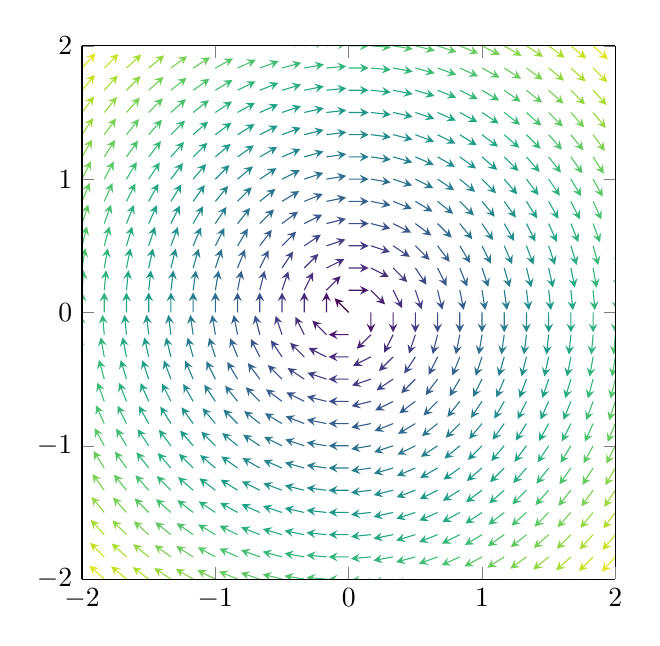
\begin{tikzpicture}
      \begin{axis}[
         xmin = -2, xmax = 2,
         ymin = -2, ymax = 2,
         zmin = 0, zmax = 1,
         axis equal image,
         xtick distance = 1,
         ytick distance = 1,
         view = {0}{90},
         scale = 1.25,
         height=7cm,
         colormap/viridis,
      ]
         \addplot3[
            point meta = {sqrt(x^2+y^2)},
            quiver = {
               u = {y/sqrt(x^2+y^2)},
               v = {-x/sqrt(x^2+y^2)},
               scale arrows = 0.15,
            },
            quiver/colored = {mapped color},
            -stealth,
            domain = -2:2,
            domain y = -2:2,
         ] {0};   
      \end{axis}
   \end{tikzpicture}
   \caption{Champs de vecteurs \( f(x, y) = (-y, x) \)}
\end{figure*}
On utilise alors un vocabulaire spécifique dans ce cadre:
\begin{itemize}
   \item On appelle \textbf{courbe intégrable} une solution maximale de l'équation.
   \item On appelle \textbf{orbite} une courbe géométrique image d'une solution de l'équation.
   \item On appelle \textbf{point stationnaire} les points tels que le champs de vecteur s'annule.
   \item On appelle \textbf{iscolines} les points tels qu'une des composantes du champs de vecteurs s'annulent.
\end{itemize}
On peut alors montrer que dans ce cadre particulier, si deux solutions maximales \( y_1, y_2 \) ont un point commun, alors elles sont \textbf{translatées} l'une de l'autre, et en conséquences, elles ont la même orbite. En outre la justification du terme d'orbite sera justifiée plus loin.
\subsection*{\subsecstyle{Flot réduit{:}}}
Dans ce cadre le flot se réduit simplement car si \( y_{t_0, y_0} \) est une solution maximale, alors la fonction translatée \( y_{0, y_0}(t + t_0)\) vérifie la même condition. En outre, quitte à translater, se ramener à l'étude des solutions maximales pour les conditions initiales \( (0, y_0) \). Par suite, le \textbf{flot réduit} de ce type d'équation s'écrit donc:
\[ 
   \begin{aligned}
      \Phi : D &\longrightarrow \K^n \\
      (t, y_0) &\longmapsto y_{0, y_0}(t)
   \end{aligned} 
\]
Si on fixe \( t \in \R \) et qu'on pose \( U_t = \left\{ y_0 \in \K^n \; ; \; t \in I_{0, y_0} \right\}  \), alors on peut voir le flot comme une application de la forme:
\[ 
   \begin{aligned}
      \Phi_t : U_t &\longrightarrow \K^n \\
      y_0 &\longmapsto \Phi(t, y_0) = y_{0, y_0}(t)
   \end{aligned}
\]
Qui s'intérprète alors réelement comme un opérateur d'évolution qui à un état \( y_0 \) au temps \( 0 \) associe l'état \( y_0(t) \) au temps \( t \). En particulier on montre les propriétés suivantes:
\[ 
   \begin{cases}
      \Phi_0 = \text{Id}\\
      \Phi_{t_2} \circ \Phi_{t_1} = \Phi_{t_1+t_2}\\
      \Phi_{t}^{-1} = \Phi_{-t}
   \end{cases} 
\]
Ceci définit en fait une \textbf{action du groupe} \( (\Phi_t)_{t \in \R}\) sur l'ensemble des 



   \pagebreak   

   \addcontentsline{toc}{chapter}{Géométrie} % 95%
   \chapter*{\chapterstyle{X --- Généralités}} % 
\addcontentsline{toc}{section}{Généralités}
Dans cette partie, nous appliquons les notions vues dans les chapitres d'algèbre linéaire et d'analyse vectorielle pour étudier les propriétés géométriques des ensembles géométriques de \(\R^n\). Ce partie introductive vise surtout à définir des concepts généraux récurrents pour la suite.

\subsection*{\subsecstyle{Système de coordonées{:}}}
On considère un point quelconque \(P\) de \(\R^n\), alors on sait depuis longtemps que cet espace est muni d'un système de coordonées canonique appellé "coordonées cartésiennes", cela signifie le concept suivant:
\begin{center}
   Un point \(P\) peut être caractérisé par ses coordonées cartésiennes.
\end{center}
Mais il existe d'autres systèmes de coordonées:
\begin{itemize}
   \item Dans le cas de \(\R^2\), on peut identifier un point \(P\) à sa distance à l'origine et son angle avec la demi-droite \(Ox\), ce sont les \textbf{coordonées polaires}.
   \item Dans le cas de \(\R^3\), on peut identifier un point \(P\) à ses cordonées polaires \((r, \theta)\) dans le plan \(xy\) et à sa hauteur \(z\) par rapport à ce plan, ce sont les \textbf{coordonées cylindriques}.  
   \item Dans le cas de \(\R^3\), on peut identifier un point \(P\) à sa distance à l'origine et sa latitude \(\theta\) et sa longitude \(\phi\), ce sont les \textbf{coordonées sphériques}.  
\end{itemize}
En particulier pour les considérations \textbf{géométriques}, étant donnée une fonction, équation, ou un point donnée d'un espace, il faut fixer implicitement ou explictement dans quel système de coordonées sont censés être représentés les objets car alors les propriétés sont changées. Considérons par exemple la fonction réelle suivante dont la variable est volontairement privée de toute interpretation par la notation:
\[
   f(\psi) = \psi
\]
On considère souvent implicitement que sa représentation est l'ensembles des points \((x, x)\) en cordonées cartésiennes et on obtient la première bissectrice du plan. Mais on peut tout à fait considèrer que sa représentation est l'ensemble des points \((\theta, \theta)\) en coordonées polaires et on obtient alors une spirale ! En effet la fonction elle-même ne transporte pas d'informations géométriques à priori.\<

Pour un exemple de propriété différentielle qui dépends du système de coordonées considéré, on considère le gradient de \(f\) en coordonées cartésiennes:
\[
   \nabla f = \left(\partialD{f}{x}, \partialD{f}{y}\right) 
\]

\subsection*{\subsecstyle{Représentations d'une courbe{:}}}
Une courbe \(\Gamma\) peut être représentée de différentes manières selon le contexte et les objectifs détudes:
\begin{itemize}
   \item Comme la courbe associé à un arc paramétré lorsque c'est possible.
   \item Comme une courbe de niveau d'une fonction\footnote[1]{En particulier si la fonction est polynômiale, on parlera alors de \textbf{courbe algébrique}, qui est le domaine d'étude reliant l'algèbre commutative et la géométrie.} \(f : \R^2 \rightarrow \R\) lorsque c'est possible.
   \item Comme le graphe d'une fonction \(f : \R \rightarrow \R\) lorsque c'est possible.
\end{itemize}
Les différentes représentations ont chacun leur intérêts propres, étant soit dans les propriétés géométriques ou algébriques soit dans la simplicité d'écriture, il sera utile d'être capable de jongler entre les différentes représentations d'une même courbe. De manière générale, la dernière représentation est souvent abstraite en la première par la paramétrisation évidente:
\[
   \Gamma(t) = (t, f(t))
\]

\subsection*{\subsecstyle{Représentations d'une surface{:}}}
Une surface \(\Sigma\) peut être représentée de différentes manières selon le contexte et les objectifs détudes:
\begin{itemize}
   \item Comme la surface associé à une surface paramétrée lorsque c'est possible.
   \item Comme une surface de niveau d'une fonction \(f : \R^3 \rightarrow \R\) lorsque c'est possible.
   \item Comme le graphe d'une fonction \(f : \R^2 \rightarrow \R\) lorsque c'est possible.
\end{itemize}
A nouveau, les différentes représentations ont chacun leur intérêts propres, étant soit dans les propriétés géométriques ou algébriques soit dans la simplicité d'écriture, il sera utile d'être capable de jongler entre les différentes représentations d'une même courbe. De manière générale, la dernière représentation est souvent abstraite en la première par la paramétrisation évidente:
\[
   \Sigma(u, v) = (u, v, f(u, v))
\]

\subsection*{\subsecstyle{Représentation paramétrique d'un ensemble{:}}}
Soit \(A \subseteq \R^n\) et \(x_i \in \mathcal{C}^1(\mathcal{U}, \R^p)\) avec \(n \leq p\), alors on définit la fonction vectorielle suivante:
\[
   \begin{aligned}
      f: \mathcal{U} &\longrightarrow \R^p\\
      (t_1, \ldots, t_n) &\longmapsto (x_1(t_1, \ldots, t_n), \ldots, x_p(t_1, \ldots, t_n))
   \end{aligned}
\]
On apelle alors \textbf{ensemble paramétré} le couple \((U, f)\) et \textbf{ensemble gémétrique} l'ensemble des points \(f(\mathcal{U})\).\<

Réciproquement, si on a un ensemble géométrique \(E \subset \R^p\) et qu'il existe une fonction \(f\) telle que \(f(\mathcal{U}) = E\), alors \((\mathcal{U}, f)\) est apellé \textbf{paramétrage de l'ensemble géométrique}. On définit de même les ensemble paramétrés de classe \(\mathcal{C}^k\) par le fait que \(f\) soit de classe \(\mathcal{C}^k\). \<

Les cas particuliers suivant seront les plus étudiés:
\begin{itemize}
   \item Si \(n = 1\) et \(p = 3\) on appelle l'ensemble géométrique \textbf{courbe plane}.
   \item Si \(n = 1\) et \(p = 3\) on appelle l'ensemble géométrique \textbf{courbe gauche}.
   \item Si \(n = 2\) et \(p = 3\) on appelle l'ensemble géométrique \textbf{surface paramétrée}.
\end{itemize}
Par exemple on a:
\begin{itemize}
   \item Une paramétrisation du cercle unité: \(\phi: t \in [0, 2\pi] \longmapsto (\cos(t), \sin(t))\)
   \item Une paramétrisation d'une hélice: \(\phi: t \in [0, 2\pi] \longmapsto (\cos(t), \sin(t), t)\)
   \item Une paramétrisation du cylindre: \(\phi: (u, v) \in [0, 5] \longmapsto (\cos(u), \sin(u), v)\)
\end{itemize}

\subsection*{\subsecstyle{Changements de paramétrage{:}}}
Soit \(\gamma = (A, f)\) un ensemble paramétré de classe \(\mathcal{C}^k\). Soit \(\phi\) un \(\mathcal{C}^k\)-diféomorphisme d'un certain intervalle \(B\) dans \(A\), alors on appelle la fonction \(f \circ \phi\) un \textbf{paramétrage admissible} de l'ensemble et on dit alors que les ensembles géométriques sont \(\mathcal{C}^k\)\textbf{-équivalents}.\<

Deux ensembles paramétrés \(\mathcal{C}^k\)\textbf{-équivalents} ont même ensembles géométriques, en particulier, on remarque alors qu'il existe une infinité de paramétrages d'un ensemble géométrique donné.

\subsection*{\subsecstyle{Notion de points multiples{:}}}
Si on considère un ensemble paramétré \((A, f)\), alors il est possible que l'ensemble géométrique ait des \textbf{points multiples}, ie qu'un point donné ait plusieurs antécédents. On appelera alors \textbf{multiplicité} du point le nombre de ces antécédents, et ont remarquera directement que si \(f\) est injective alors nécéssairement, elle n'a pas de points multiples.\<

On dira alors qu'un tel ensemble géométrique est \textbf{simple}.

\subsection*{\subsecstyle{Notion de points réguliers{:}}}
On considère un ensemble paramétré \((\mathcal{U}, f)\), alors:
\begin{center}
   Un point de \(\mathcal{U}\) est dit \textbf{régulier} si et seulement si \(d\Sigma_a\) est de \textbf{rang maximal}, sinon 
   
   on dira qu'il est \textbf{singulier}\footnote[1]{Attention cette notion est différente de celle de \textbf{point critique}, en effet un point peut être singulier, par exemple la différentielle d'une fonction \(f : \R^2 \rightarrow \R\) qui serait de rang \(1\), sans qu'elle soit nulle.}.
\end{center}
On dira alors que l'ensemble géométrique est \textbf{régulier} si tout ses points sont réguliers.

\subsection*{\subsecstyle{Notion de contact{:}}}
On considère deux courbes \(\Gamma, \Gamma'\) qui s'intersectent en un point \(a\), alors on dira qu'elles ont un contact d'ordre 0, et on définit alors un raffinement de la notion de contact entre deux courbes en définissant le notion de contact d'ordre \(p\).\<

On dira que deux courbes ont un contact d'ordre \(p\) si leurs développements limités à l'ordre \(p\) au point considéré coincident. Cela signifie intuitivement que la qualité du contact est meilleure, en effet deux courbes ayant un contact d'ordre \(1\) sont tangentes, et partagent donc même développement limité à l'ordre \(1\).\<

Dans le cas des surfaces, il faut alors considérer les développements de Taylor des fonctions à plusieurs variables (ou paramétrisations) considérés et la définition précédente se généralise.
\chapter*{\chapterstyle{X --- Courbes planes I}} % 
\addcontentsline{toc}{section}{Courbes planes I}

Dans ce chapitre, on s'intéresse au cas particuliers des \textbf{courbes planes} et à leur propriétés métriques et différentielles élémentaires. Dans tout la suite, les arcs paramétrés seront supposés de classe \(\mathcal{C}^1\) et \textbf{réguliers}.

\subsection*{\subsecstyle{Courbes planes remarquables{:}}}
On peut considèrer alors quelques courbes remarquables:
\begin{figure}[h]
   \centering
   \begin{subfigure}{.3\textwidth}
      \centering
      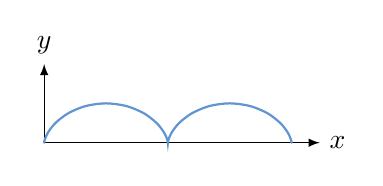
\begin{tikzpicture}[line cap=round]
         \draw[-latex] (0,0) -- (3.5,0) node [right] {$x$};
         \draw[-latex] (0, 0)     -- (0,1) node [above] {$y$};
         \draw[BrightBlue1, thick] plot[variable=\t,domain=0:4*pi,smooth,thick] ({(\t - sin(\t r))/4},{(1 - cos(\t r))/4});
      \end{tikzpicture}
      \caption*{La cycloïde}
   \end{subfigure}\quad
   \begin{subfigure}{.3\textwidth}
      \centering
      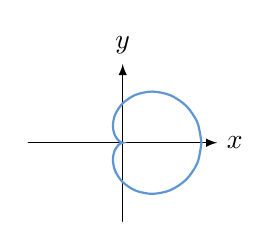
\begin{tikzpicture}[line cap=round]
         \draw[-latex] (-1.2,0) -- (1.2,0) node [right] {$x$};
         \draw[-latex] (0,-1)     -- (0,1) node [above] {$y$};
         \draw[BrightBlue1, thick] plot[variable=\t,domain=0:2*pi,smooth,thick] ({(cos(\t r)+1)*(cos(\t r)/2},{(cos(\t r)+1)*(sin(\t r)/2});
      \end{tikzpicture}
      \caption*{Une cardioïde}
   \end{subfigure}\quad
   \begin{subfigure}{.3\textwidth}
      \centering
      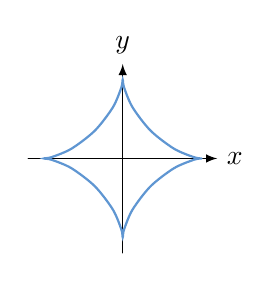
\begin{tikzpicture}[line cap=round]
         \draw[-latex] (-1.2,0) -- (1.2,0) node [right] {$x$};
         \draw[-latex] (0,-1.2)     -- (0,1.2) node [above] {$y$};
         \draw[BrightBlue1, thick] plot[variable=\t,domain=0:2*pi,smooth,thick] ({(cos(\t r)^3)},{(sin(\t r)^3)});
      \end{tikzpicture}
      \caption*{Une hypocycloïde}
   \end{subfigure}\quad
   \begin{subfigure}{.3\textwidth}
      \centering
      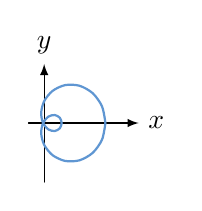
\begin{tikzpicture}[line cap=round]
         \draw[-latex] (-0.2,0) -- (1.2,0) node [right] {$x$};
         \draw[-latex] (0,-0.75)     -- (0,0.75) node [above] {$y$};
         \draw[BrightBlue1, thick] plot[variable=\t,domain=0:2*pi,smooth,thick] ({(1/1.8+cos(\t r))/2*cos(\t r)},{(1/2+cos(\t r))/1.8*sin(\t r)});
      \end{tikzpicture}
      \caption*{Un limaçon}
   \end{subfigure}\quad
   \begin{subfigure}{.3\textwidth}
      \centering
      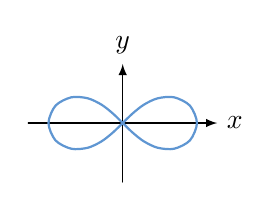
\begin{tikzpicture}[line cap=round]
         \draw[-latex] (-1.2,0) -- (1.2,0) node [right] {$x$};
         \draw[-latex] (0,-0.75)     -- (0,0.75) node [above] {$y$};
         \draw[BrightBlue1, thick] plot[variable=\t,domain=0:2*pi,smooth,thick] ({(sqrt(2)/1.5*sin(\t r))/(1+cos(\t r)^2)},{(sqrt(2)/1.5*sin(\t r)*cos(\t r))/(1+cos(\t r)^2)});
      \end{tikzpicture}
      \caption*{Le lemniscate de Bernoulli}
   \end{subfigure}\quad
   \begin{subfigure}{.3\textwidth}
      \centering
      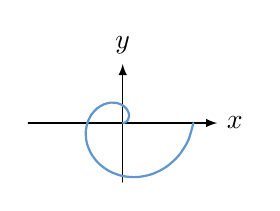
\begin{tikzpicture}[line cap=round]
         \draw[-latex] (-1.2,0) -- (1.2,0) node [right] {$x$};
         \draw[-latex] (0,-0.75)     -- (0,0.75) node [above] {$y$};
         \draw[BrightBlue1, thick] plot[variable=\t,domain=0:2*pi,smooth,thick] ({\t/7*cos(\t r)},{\t/7*sin(\t r)});
      \end{tikzpicture}
      \caption*{La spirale d'Archimède}
   \end{subfigure}\quad
\end{figure}

Ces courbes ont des propriétés trés intéressantes et se retrouvent, par exemple, en physique. En effet, la cycloïde (inversée) représente la pente qui minimise le temps de trajet d'une bille lancée en haut de celle ci. On dit que c'est une courbe \textbf{brachistochrone}.

\subsection*{\subsecstyle{Longueur de courbes paramétrées{:}}}
On s'intéresse à la \textbf{longueur de l'arc paramétré} \((I, \gamma)\) qu'on notera \(L\).\<

On peut alors subdiviser \(I\) en différents intervalles et approximer la longueur de l'arc par la somme des cordes d'extérmités les différentes subdivisions. En faisant alors tendre la longueur des subdivisions vers 0, on obtient, à la limite, une intégrale de Riemann\footnote[1]{L'intégrande est bien intégrable (et même continue) en tant que somme produit et composées de fonctions intégrables (continues)}, et la définition suivante:
\customBox{width=3.5cm}{
   \[
      L := \int_I \vectNorm{\gamma'(t)}\, dt  
   \]
}
On appelle alors \textbf{abcisse curviligne} d'origine \(t_0\), ou encore fonction longeur d'arc, la primitive:
\[
   s(t) = \int_{t_0}^{t} \vectNorm{\gamma'(x)} \d x
\]
Par exemple dans \(\R^2\) pour l'arc paramétré \((I, \gamma)\) avec \(I = \icc{0}{1}\) et \(\gamma(t) = (t, t^2)\), on obtient:
\[
   L := \int_{I} \vectNorm{\gamma'(t)}\,dt = \int_{\icc{0}{1}} \vectNorm{(1, 2t)}\,dt = \int_{\icc{0}{1}}\sqrt{1 + 4t^2}\,dt \approx 1.47
\]
\pagebreak

On peut aussi préfèrer exprimer la longeur d'arc en coordonées polaires, alors on peut déduire\footnote[1]{A partir de \((x(t), y(t)) = (r(t)\cos(t), r(t)\sin(t))\), il suffit de calculer la norme du vecteur dérivée en fonction de \(r(t)\).} de la définition ci-dessus la caractérisation suivante:
\customBox{width=5cm}{
   \[
      L := \int_I \sqrt{r'(\theta)^2 + r(\theta)^2}\, d\theta 
   \]
}

\subsection*{\subsecstyle{Aires de courbes paramétrées{:}}}
On s'intéresse à \textbf{l'aire entre l'arc paramétré} \((I, \gamma)\) et l'axe des abcisses qu'on notera \(A\).

On peut alors subdiviser \(I\) et approximer l'aire sous la courbe par la somme d'aires de rectangles. En faisant alors tendre la longueur des subdivisions vers 0, on obtient une intégrale de Riemann\footnote[2]{L'intégrande est bien intégrable en tant que somme produit et composées de fonctions intégrables.}, et la définition suivante:
\customBox{width=3.8cm}{
   \[
      A := \int_I y(t)x'(t)\, dt
   \]
}
Par exemple pour l'arc paramétré \((I, \gamma)\) avec \(I = \icc{0}{1}\) et \(\gamma(t) = (t, t^2)\), on obtient:
\[
   A := \int_I y(t)x'(t)\, dt = \int_{\icc{0}{1}} t^2\, dt = \frac{1}{3}
\]

Dans le cas des courbes en coordonées polaires, on peut calculer l'aire bornée par la courbe, on subdivise alors \(I\) en \((\theta_i)_{i \in \N}\), et on calcule la somme de \textbf{secteurs circulaires} de rayon \(r(\theta_k)\). Or on sait que l'aire d'une cercle de rayon \(r\) est donnée par \(\pi r^2\) donc l'aire d'un secteur circulaire d'angle \(\theta\) est donné par \(A = \frac{1}{2}\theta r^2\).\<

Pour obtenir l'aire délimitée par la courbe polaire on peut alors sommer les aires des secteurs circulaires, on obtient alors, à la limite, une intégrale de Riemann et la définition suivante:
\customBox{width=4cm}{
   \[
      A := \frac{1}{2} \int_I r(\theta)^2\, d\theta
   \]
}
\begin{center}
   \textit{
      On a alors deux types de calculs d'aires, l'aire des rectangles entre une courbe et l'axe des abcisses et l'aire des secteurs circulaires entre une courbe et l'origne, qui ne sont \textbf{pas du tout équivalentes}.
   }
\end{center}

\subsection*{\subsecstyle{Paramétrage normal{:}}}
Si \(s\) est l'abcisse curviligne d'un arc \((I, \gamma)\) de classe \(\mathcal{C}^1\), alors on peut montrer\footnote[3]{Elle est continue et strictement croissante et sa dérivée ne s'annule pas, donc bijective à réciproque dérivable. Voir le chapitre sur la dérivation, partie ``Dérivée d'une réciproque''.} que \(s\) est un \(\mathcal{C}^1\)-difféomorphisme de \(I\) sur \(J = \gamma(I)\), et en particulier, on peut alors reparamétrer par l'abcisse curviligne et obtenir:
\customBox{width=5cm}{
   \(
      (I, \gamma) \sim (J, \gamma \circ s^{-1})
   \)
}
On peut alors remarquer alors que ce nouvel arc paramétré s'affranchit de la vitesse de parcours, et parcours la courbe \textbf{à vitesse constante}. Ce reparamétrage appelée \textbf{paramétrage normal} est généralement bien plus naturel quand on s'intéresse à des questions géométriques intrinsèques à la courbe.
\chapter*{\chapterstyle{X --- Courbes planes II}} % 
\addcontentsline{toc}{section}{Courbes planes II}
Dans ce chapitre, on s'intéresse à l'étude de propriétés métriques des \textbf{courbes planes} plus subtiles. Nous avons déja défini la notion de longueur d'arc précédemment, dans ce chapitre, nous défiront le \textbf{repère de Frenet} et nous développeront le concept de \textbf{courbure algébrique}, de \textbf{cercle osculateur}, et de \textbf{développée} d'une courbe plane.

\subsection*{\subsecstyle{Repère de Frenet{:}}}
Dans tout la suite, on se donne un arc paramétré \((\gamma, I)\) de classe \(\mathcal{C}^2(I)\) de courbe \(\Gamma\). On définit tout d'abord un vecteur tangent unitaire:
\[
   T(t) = \frac{\gamma'(t)}{\vectNorm{\gamma'(t)}}
\]
L'idée du repère de Frenet est alors de définir un \textbf{repère mobile d'orientation directe}, donc on définit un vecteur \(N(t)\) normal à \(T(t)\) tel que le repère \(T(t), N(t)\) soit un repère orthonormé direct, ie on a:
\[
   N(t) := R_\frac{\pi}{2}T(t) = \begin{pmatrix} 0 & -1\\ 1 & 0\end{pmatrix} T(t) 
\]
Le couple \((T(t), N(t))\) est alors appelé \textbf{repère (mobile) de Frenet}, on abrège souvent les notations de dépendance en \(t\) et on note alors ce repère \((T, N)\).

\subsection*{\subsecstyle{Courbure{:}}}
On paramétre à présent l'arc par son abcisse curviligne \(s\), on peut alors montrer par calcul direct que \(T'(s) \perp T(s) \) et en particulier, on a donc que le vecteur accélération \(T'(s)\) est colinéaire à \(N(s)\), et il existe donc un scalaire \(\kappa(s)\) tel que:
\[
   dT(s) = \kappa(s)N(s)ds
\]
On peut aussi montrer par calcul direct que \(N'(s) \perp N(s) \) et en particulier, on a donc que le vecteur \(N'(s)\) est colinéaire à \(T(s)\), et pour le même scalaire \(\kappa(s)\) on a:
\[
   dN(s) = -\kappa(s)T(s)ds
\]
On donne alors à \(\kappa(s)\) le nom de \textbf{courbure algébrique} au point \(\gamma(s)\). Sa valeur absolue mesure à quel point la courbe est courbée, et son signe donne la direction du virage par rapport au sens de parcours:
\begin{itemize}
   \item Si elle est positive, la courbe tourne à gauche.
   \item Si elle est négative, la courbe tourne à droite.
\end{itemize}
En particulier les formules ci-dessus sont appellées \textbf{formules de Frenet}, et par manipulation des différentielles et en notant \(v(t)\) la vitesse scalaire, on obtient un équivalent pour un paramétrage quelconque donné par:
\[
   \begin{cases}
      dT(t) = v(t)\kappa(t)N(t)dt\\
      dN(t) = -v(t)\kappa(t)N(t)dt\\
   \end{cases}   
\]
\subsection*{\subsecstyle{Courbure totale{:}}}
On considère une courbe \textbf{fermée} paramétrée par \((I, \gamma)\), alors on peut définir la \textbf{courbure totale} de la courbe par:
\[
   \int_I\kappa(t)v(t)dt   
\]
Dans le cas d'une courbe fermée, c'est un multiple de \(2\pi\) qui donne le nombre de tours effectués.
\pagebreak

\subsection*{\subsecstyle{Cercle osculateur{:}}}
On définit le concept de \textbf{cerlce osculateur} en un point \(\gamma(t)\) par la propriété suivante:
\begin{center}
   \textbf{Le cercle osculateur est l'unique cercle ayant un contact d'ordre au moins 2 en ce point.}
\end{center}
On définit alors le \textbf{rayon de courbure algébrique} comme étant l'inverse de la courbure et on montre que la position du centre du cercle osculateur est paramétré par:
\[
   C(t) = \gamma(t) + \frac{1}{\kappa(t)}N(t) 
\] 
Géométriquement, c'est le point à distance le rayon de courbure dans la direction de \(N(t)\), on peut alors vérifier que si on paramétre le cercle osculateur de la sorte, le contact est bien d'ordre au moins 2.\< 

L'ensemble des tels centres de courbures, c'est à dire la courbe \(\Gamma'\) de l'arc paramétré \((I, C)\) est appelé \textbf{développée} de la courbe \(\Gamma\) et \(\Gamma\) est appelé \textbf{développante} de la courbe \(\Gamma'\).

\subsection*{\subsecstyle{Théorème de l'accélération normale{:}}}
On cherche maintenant une expression du vecteur accélération \(A(t)\) dans la base \((T, N)\), on a tout d'abord la formule suivante:
\[
   \gamma'(t) = v(t)T(t) 
\]
Où on note à nouveau \(v(t)\) la vitesse scalaire. On cherche donc une expression du vecteur accélération, donc on dérive cette expression et on obtient:
\begin{flalign*}
   \gamma''(t) &= (v(t)T(t))' \Longleftrightarrow \\
   &= v'(t)T(t) + v(t)T'(t) \Longleftrightarrow \\
   &= v'(t)T(s(t)) + v^2(t)\kappa(t)N(t) \Longleftrightarrow \shorteqnote{(D'aprés les formules de Frenet dans un paramétrage quelconque.)} \\
   &= a_T(t)T(s(t)) + a_N(t)N(t)
\end{flalign*}
Alors on peut en déduire une interprétation cinématique puissante, on décompose en effet ici l'accélaration en ses \textbf{composantes tangentielles et normales}. 
\begin{center}
   \textit{
      Cela démontre en particulier que l'accélaration normale est proportionnelle au carré de la vitesse, ie que si on va deux fois plus vite dans un virage, l'accélération subie dans la direction du centre de rotation est quatre fois plus intense.
   }
\end{center}
De manière plus pragmatique, cela donne par ailleurs un moyen simple de calculer la courbure, en effet on en déduit l'expression suivante:
\[
   \kappa(t) = a_N(t)\frac{1}{v^2(t)} = \dotproduct{\gamma''(t)}{N(t)}\frac{1}{v^2(t)}   
\]
Où toutes les quantités sont aisément calculables.
\chapter*{\chapterstyle{X --- Courbes gauches}} % 
\addcontentsline{toc}{section}{Etude métriques des courbes gauches}
Dans ce chapitre, on s'intéresse à l'étude des propriétés métriques des \textbf{courbes gauches}, c'est à dire des courbes se situant dans \(\R^3\).

Il est tout d'abord important de noter que la notion de longueur d'arc et d'abcisse curviligne d'une courbe plane se généralise directement dans le cas des courbes gauches. Dans ce chapitre, nous défiront le \textbf{trièdre de Frenet} et nous développeront le concept de \textbf{courbure}, de \textbf{torsion} et de \textbf{plan osculateur} d'une courbe gauche.
\chapter*{\chapterstyle{X --- Surfaces Paramétrés}} % 
\addcontentsline{toc}{section}{Surfaces Paramétrés}

Dans ce chapitre, on s'intéresse au cas particulier des \textbf{surfaces} de \(\R^3\). Dans tout la suite, on considérera les surfaces considérés de classe \(\mathcal{C}^1\) et \textbf{régulières}.

\subsection*{\subsecstyle{Surface planes remarquables A FAIRE{:}}}
On peut considèrer alors quelques courbes remarquables:
\begin{figure}[h]
   \centering
   \begin{subfigure}{.3\textwidth}
      \centering
      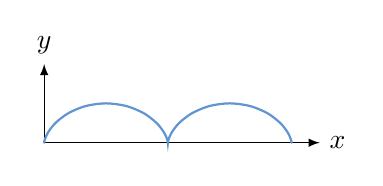
\begin{tikzpicture}[line cap=round]
         \draw[-latex] (0,0) -- (3.5,0) node [right] {$x$};
         \draw[-latex] (0, 0)     -- (0,1) node [above] {$y$};
         \draw[BrightBlue1, thick] plot[variable=\t,domain=0:4*pi,smooth,thick] ({(\t - sin(\t r))/4},{(1 - cos(\t r))/4});
      \end{tikzpicture}
      \caption*{La cycloïde}
   \end{subfigure}\quad
   \begin{subfigure}{.3\textwidth}
      \centering
      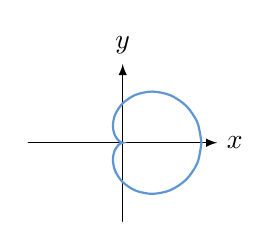
\begin{tikzpicture}[line cap=round]
         \draw[-latex] (-1.2,0) -- (1.2,0) node [right] {$x$};
         \draw[-latex] (0,-1)     -- (0,1) node [above] {$y$};
         \draw[BrightBlue1, thick] plot[variable=\t,domain=0:2*pi,smooth,thick] ({(cos(\t r)+1)*(cos(\t r)/2},{(cos(\t r)+1)*(sin(\t r)/2});
      \end{tikzpicture}
      \caption*{Une cardioïde}
   \end{subfigure}\quad
   \begin{subfigure}{.3\textwidth}
      \centering
      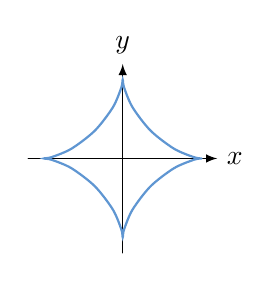
\begin{tikzpicture}[line cap=round]
         \draw[-latex] (-1.2,0) -- (1.2,0) node [right] {$x$};
         \draw[-latex] (0,-1.2)     -- (0,1.2) node [above] {$y$};
         \draw[BrightBlue1, thick] plot[variable=\t,domain=0:2*pi,smooth,thick] ({(cos(\t r)^3)},{(sin(\t r)^3)});
      \end{tikzpicture}
      \caption*{Une hypocycloïde}
   \end{subfigure}\quad
   \begin{subfigure}{.3\textwidth}
      \centering
      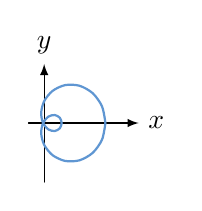
\begin{tikzpicture}[line cap=round]
         \draw[-latex] (-0.2,0) -- (1.2,0) node [right] {$x$};
         \draw[-latex] (0,-0.75)     -- (0,0.75) node [above] {$y$};
         \draw[BrightBlue1, thick] plot[variable=\t,domain=0:2*pi,smooth,thick] ({(1/1.8+cos(\t r))/2*cos(\t r)},{(1/2+cos(\t r))/1.8*sin(\t r)});
      \end{tikzpicture}
      \caption*{Un limaçon}
   \end{subfigure}\quad
   \begin{subfigure}{.3\textwidth}
      \centering
      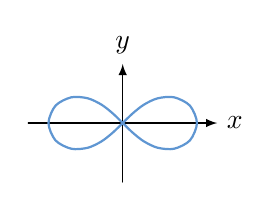
\begin{tikzpicture}[line cap=round]
         \draw[-latex] (-1.2,0) -- (1.2,0) node [right] {$x$};
         \draw[-latex] (0,-0.75)     -- (0,0.75) node [above] {$y$};
         \draw[BrightBlue1, thick] plot[variable=\t,domain=0:2*pi,smooth,thick] ({(sqrt(2)/1.5*sin(\t r))/(1+cos(\t r)^2)},{(sqrt(2)/1.5*sin(\t r)*cos(\t r))/(1+cos(\t r)^2)});
      \end{tikzpicture}
      \caption*{Le lemniscate de Bernoulli}
   \end{subfigure}\quad
   \begin{subfigure}{.3\textwidth}
      \centering
      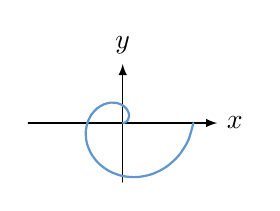
\begin{tikzpicture}[line cap=round]
         \draw[-latex] (-1.2,0) -- (1.2,0) node [right] {$x$};
         \draw[-latex] (0,-0.75)     -- (0,0.75) node [above] {$y$};
         \draw[BrightBlue1, thick] plot[variable=\t,domain=0:2*pi,smooth,thick] ({\t/7*cos(\t r)},{\t/7*sin(\t r)});
      \end{tikzpicture}
      \caption*{La spirale d'Archimède}
   \end{subfigure}\quad
\end{figure}

Ces courbes ont des propriétés trés intéressantes et se retrouvent, par exemple, en physique. En effet, la cycloïde (inversée) représente la pente qui minimise le temps de trajet d'une bille lancée en haut de celle ci. On dit que c'est une courbe \textbf{brachistochrone}.

\subsection*{\subsecstyle{Aire d'une surface paramétrée A FAIRE{:}}}
\chapter*{\chapterstyle{X --- Etude des équations coniques}} % 
On appelle \textbf{conique} tout courbe algébrique dont les points \((x, y) \in E\) vérifiant une égalité de la forme:
\[
   Ax^2 + Bxy + Cy^2 + Dx + Ey + F = 0  
\]
Avec \(A, B, C\) non tous nuls. Cette ensemble représente alors \textbf{l'intersection} obtenue en coupant un cone par un plan. On obtient alors trois types de coniques non-dégénérées\footnote[1]{Les formes dégénérées sont aisément reconnues aprés le premier changement de repère ci-dessous, on s'intéresse donc uniquement aux formes non-dégénérées.}:
\begin{itemize}
   \item Les ellipses
   \item Les paraboles
   \item Les hyperboles
\end{itemize}
On cherche alors à caractériser ces courbes algébriquement ou géométriquement. En première approche, on pourra déja reconnaitre que ces coniques admettent au moins un axe de symétrie, et un centre de symétrie pour les ellipses et les hyperboles.

\subsection*{\subsecstyle{Réduction}}
L'ensembe des coniques est stable par changement de repère. Aussi, on peut exprimer matriciellement ces équations par:
\[
   \begin{pmatrix}x & y\end{pmatrix}\begin{pmatrix}
      A & \frac{B}{2} \\
      \frac{B}{2} & C
   \end{pmatrix} \begin{pmatrix}x \\ y\end{pmatrix} + \begin{pmatrix}D & E\end{pmatrix} \begin{pmatrix}x \\ y\end{pmatrix} + F = 0
\]
La raison principale étant alors qu'on peut alors classifier de telles coniques en étudiant la \textbf{positivité} de la matrice symétrique associée \(Q\), en effet:
\begin{itemize}
   \item Si \(\det({Q}) > 0\) et que \(F\) est négatif, alors on obtient une \textbf{ellipse}.
   \item Si \(\det({Q}) = 0\) alors on obtient une \textbf{parabole}.
   \item Si \(\det({Q}) < 0\), alors on obtient une \textbf{hyperbole}.
\end{itemize}

En effet, le signe du déterminant d'un matrice de cette taille caractérise exactement le signe des valeurs propres et donc la forme de l'équation finale car si on pose alors \(\lambda, \mu\) les valeurs propres de cette matrice\footnote[2]{Si \(\mu\) est nulle est qu'on a une parabole, alors la forme est évidente.}, et qu'on pose le changement de variable:
\[
   \begin{pmatrix}X \\ Y\end{pmatrix} = P^{-1} \begin{pmatrix}x \\ y\end{pmatrix}
\]
\begin{center}
   \textit{Ce changement de variable revient à effectuer une rotation du repère pour aligner les axes avec les axes de symétrie de la conique (qui sont alors les vecteurs propres).}
\end{center}
On obtient alors directement l'équation plus simple avec \(\alpha, \beta\) les nouveaux coefficients des termes en \(X, Y\):
\[
   \lambda X^2 + \mu Y^2 + \alpha X + \beta Y + F = 0 
\]

Si on met alors sous forme canonique les deux parties de l'équation, on obtient:
\[
   \lambda(X + t_1)^2 + \mu (Y + t_2)^2 + F = 0 
\]
Finalement aprés un nouveau changement de repère obtenu par translation de \((t_1, t_2)\), on obtient alors l'équation:
\[
   \lambda\tilde{X}^2 + \mu\tilde{Y}^2 = -F
\]
\pagebreak

Finalement, on peut toujours se ramener à une \textbf{équation réduite} de la forme:
\[
   \left(\frac{\tilde{X}}{a}\right)^2 + \left(\frac{\tilde{Y}}{b}\right)^2 = 1
\]
Et on trouve alors facilement les éléments caractéristiques la conique:
\begin{itemize}
   \item Son centre (s'il existe), situé en \((0, 0)\) en coordonées \((\tilde{X}, \tilde{Y})\)
   \item Ses sommets (s'ils existent), situés en \((\pm a, 0), (0, \pm b)\) en coordonées \((\tilde{X}, \tilde{Y})\)
\end{itemize}
On peut aussi étudier les asymptotes dans le cas de l'hyperbole, en effet on considère alors:
\begin{flalign*}
   \left(\frac{\tilde{X}}{a}\right)^2 - \left(\frac{\tilde{Y}}{b}\right)^2 = 1 &\Longleftrightarrow
   \left(\frac{\tilde{Y}}{b}\right)^2 = \left(\frac{\tilde{X}}{a}\right)^2 - 1 \\
   &\Longleftrightarrow \tilde{Y}^2 = \frac{b^2}{a^2}\tilde{X}^2 - b^2\\
   &\Longleftrightarrow \tilde{Y} = \pm \frac{b}{a} \sqrt{\tilde{X}^2 - b^2}
\end{flalign*}
Alors aymptotiquement, quand \(x\) est trés grand, \(b^2\) est négligeable et l'hyperbole se rapproche alors des deux droites:
\[
   \tilde{Y} = \pm \frac{b}{a}\tilde{X}
\]
Reste alors à utiliser les relations entre les repères pour obtenir les asymptotes dans le repère canonique.

\subsection*{\subsecstyle{Caractérisations géométriques}}
Tout d'abord pour les coniques non-paraboliques, on a la caractérisation \textbf{bifocale} suivante, on considère deux points \(F_1, F_2\) du plan, un point \(X\) et un réel strictement positif \(d\), alors on a:
\begin{itemize}
   \item Si \(d > d(A, B)\), alors l'ensemble des points \(X\) qui vérifient \(d(F_1, X) + d(F_2, X) = d\) est une \textbf{ellipse}.
   \item Si \(d < d(A, B)\), alors l'ensemble des points \(X\) qui vérifient \(|d(F_1, X) - d(F_2, X)| = d\) est une \textbf{hyperbole}.
\end{itemize}

Dans le cas parabolique, on a la caractérisation \textbf{monofocale} suivante, on considére une droite \(\mathcal{D}\) et un point \(F\) et on a:
\begin{center}
   L'ensemble des points \(X\) qui vérifient \(d(F, X) = d(\mathcal{D}, X)\) est une \textbf{parabole}.
\end{center}
On retrouve facilement ces caractérisations en explicitant les distances considérées et en simplifiant l'équation obtenue. On peut alors prouver diverses propriétés géométriques des coniques, par exemple et de manière non exhaustive:
\begin{itemize}
   \item Si des rayons lumineux tombent de l'infini et rebondissent sur une parabole, ils se rencontrent tous en le foyer.
   \item Deux paraboles de meme foyer et de meme axe se coupent à angle droit.
   \item Si un rayon lumineux part d'un foyer d'une ellipse et rebondit sur celle-ci, il passera par l'autre foyer.
\end{itemize}

\subsection*{\subsecstyle{Coniques projectives}}

\chapter*{\chapterstyle{X --- Etude des équations quadriques}} % 

   \pagebreak   
   
   \addcontentsline{toc}{chapter}{Theorie de la mesure} % A FAIRE
   \chapter*{\chapterstyle{XI --- Introduction}} % A REFAIRE
\addcontentsline{toc}{section}{Introduction} 
Dans ce chapitre, on cherchera à définir un notion analytique qui généralise le concept de \textbf{continuité} et \textbf{d'espaces topologiques} en une notion plus générale et qui permettra de démontrer des théorèmes plus généraux et plus puissants ainsi que de développer une théorie de l'intégration plus générale et qui permettra d'intégrer sur des espaces plus complexes.\<

On appelera alors ces fonctions des fonctions \textbf{mesurables} et les espaces considérés les \textbf{espaces mesurables}.

\subsection*{\subsecstyle{Inconvénients de la notion de continuité{:}}}
La notion de continuité présente plusieurs problèmes analytiques profonds:
\begin{itemize}
   \item La limite d'une suite de fonctions continues ne l'est pas forcément.
   \item La limite d'une suite de fonctions Riemann-intégrables ne l'est pas forcément.
   \item La limite d'une suite d'intégrales n'est pas nécessairement l'intégrale de la limite.
   \item L'intégrale sur une partie non-compacte est péniblement gérée par les intégrales généralisées dans les cas simples.
   \item L'intégrale sur un segment d'une fonction trés irrégulière n'est souvent pas définie.
   \item L'espace des fonctions Riemann-intégrables n'a pas de structure forte.
\end{itemize}
De manière générale, quand on considère des objets trés réguliers (fonctions définies sur des compacts, limites uniformes de suites de fonctions, intégrale sur des domaines compacts), la continuité permet d'obtenir les résultats souhaités mais dans des cas plus exotiques, elle n'est plus suffisante. Considérons par exemple:
\[
   \begin{aligned}
      f : I = \icc{a}{b} &\longrightarrow \R \\
      x &\longmapsto \1_\Q(x)
   \end{aligned}
\]
Où \(\1_\Q\) désigne la fonction indicatrice des rationnels, alors on montre facilement que cette fonction n'est pas intégrable au sens de Riemann, en effet on a \(\displaystyle\int_I^-{f} = 0 \neq 1 = \displaystyle\int_I^+{f}\), mais on pourra définit cette intégrale gràce à la théorie de Lebesgue.
\chapter*{\chapterstyle{XI --- Espaces Mesurables}} % A REFAIRE
\addcontentsline{toc}{section}{Espaces Mesurables} 
On définit tout d'abord dans ce chapitre le concept fondamental de \textbf{tribu} sur un ensemble, qui est un concept analogue à celui de topologie, mais beaucoup moins restrictif, les morphismes de tels espaces seront alors les fonctions mesurables, en lieu et place des fonctions continues.

\subsection*{\subsecstyle{Définition {:}}}
On se donne un ensemble \(E\), on appelle \textbf{tribu} sur \(E\) tout ensemble de parties \(\mathcal{A}\) qui vérifie:
\begin{itemize}
   \item L'ensemble vide et total appartient à \(\mathcal{A}\).
   \item La tribu est \textbf{stable par passage au complémentaire}.
   \item La tribu est \textbf{stable par union dénombrable}.
\end{itemize}
On appelle le couple \((E, \mathcal{A})\) un espable mesurable et les éléments de la tribu parties mesurables.

\subsection*{\subsecstyle{Exemples de tribus {:}}}
On peut alors construire plusieurs exemples simples de tribu sur \(E\):
\begin{itemize}
   \item La tribu \(\{\emptyset, E\}\) appelée \textbf{tribu grossière}.
   \item La tribu \(\mathcal{P}(E)\) appelée \textbf{tribu discrète}.
\end{itemize}

\subsection*{\subsecstyle{Notion de finesse {:}}}
On définit alors une notion de comparaison entre deux tribus \(\mathcal{A}_1\) et \(\mathcal{A}_2\), et on dira que \(\mathcal{A}_2\) est \textbf{plus fine} que \(\mathcal{A}_1\) si et seulement si on a:
\[
   \mathcal{A}_1 \subseteq \mathcal{A}_2
\]
Cela signifie moralement que \(\mathcal{A}_2\) à plus d'ensembles mesurables, par exemple la tribu discrète est la plus fine de tout les topologies. Cette relation définit alors \textbf{une relation d'ordre} sur l'ensemble des tribus.

\subsection*{\subsecstyle{Tribu engendrée {:}}}
On se donne \(A\) un ensemble de parties de \(E\), alors on chercher à savoir si il existe une plus petite tribu (au sens de l'inclusion) telle que les éléments de \(A\) soit mesurables, ie la tribu la moins fine qui contienne \(A\).\<

On peut alors montrer facilement que l'intersection de deux tribus est une tribu et donc que la plus petite tribu qui contienne \(A\) existe, c'est l'intersection de toutes les tribu qui contiennent \(A\). On l'appelera alors \textbf{tribu engendrée} par \(A\).

\subsection*{\subsecstyle{Tribu induite {:}}}
Soit \(P \subseteq E\), alors \(E\) induit une tribu naturelle sur \(P\) appellée \textbf{tribu induite} définie par:
\[ 
   \mathcal{A}_P := \Bigl\{ A \cap \mathcal{M} \; ; \; \mathcal{M} \subseteq \mathcal{A} \Bigl\}  
\]
\begin{center}
   \textit{Une partie mesurable de \(P\) pour la tribu induite est simplement la trace sur \(P\) des parties mesurables de \(E\).}
\end{center}
\pagebreak

\subsection*{\subsecstyle{Tribu borélienne {:}}}
On considère maintenant que \(E\) n'est plus quelconque mais muni d'une \textbf{topologie} \(\mathcal{T}\), alors on définit la \textbf{tribu borélienne} sur \(E\) comme étant la tribu \textbf{engendrée par les ouverts de la topologie}. On appele alors les parties mesurables pour cette tribu les \textbf{boréliens}.\<

Par exemple voici une liste non exhaustive d'exemples sur \(\R\) de boréliens :
\begin{itemize}
   \item Les intevalles ouverts et fermés et leurs unions.
   \item Les singletons.
   \item Les intervalles semi-ouverts comme union singleton/intervalle ouvert.
   \item Les ensembles finis.
   \item Les ensembles dénombrables.
\end{itemize}
On voit alors que la tribu des boréliens contient \textbf{beaucoup de parties}, en particulier (hautement non-trivial), elle a la cardinalité de \(\R\).
\chapter*{\chapterstyle{XI --- Espaces Mesurés}} % A REFAIRE
\addcontentsline{toc}{section}{Espaces Mesurés} 

Dans ce chapitre on définit le premier concept fondamental qui ne permettra de mesurer le "volume" d'une partie complexe d'un espace mesurable, en particulier, on appelera \textbf{mesure} sur l'espace mesurable \((X, \mathscr{A})\) tout fonction \(\mu : \mathscr{A} \longrightarrow \overline{\R}_+\) qui vérifie les deux propriétés suivantes:
\begin{itemize}
   \item \textbf{Mesure du vide:} \(\mu(\emptyset) = 0\)
   \item \textbf{Sigma additivité:} \(\mu\left(\bigcup A_i\right) = \sum \mu\left(A_i\right)\) pour toute famille \textbf{dénombrable disjointe}. 
\end{itemize}
On appelle alors le triplet \((X, \mathscr{A}, \mu)\) \textbf{espace mesuré} et en particulier si \(\mu(X) = 1\), on l'appele alors \textbf{espace probabilisé} et on dira alors que \(\mu\) est une mesure de probabilité.
\subsection*{\subsecstyle{Propriétés {:}}}
On peut alors montrer les propriétés suivantes des mesures sur un espace mesurable:
\begin{itemize}
   \item \textbf{Croissance:} \(A \subseteq B \implies \mu(A) \leq \mu(B)\)
   \item \textbf{Sous-additivité:} \(\mu\left(\bigcup A_i\right)\leq \sum \mu\left(A_i\right)\) pour une famille dénombrable de parties quelconques.
   \item \textbf{Limite de mesure croissante:} \(\lim_{n \rightarrow +\infty} \mu(A_n) = \mu\left(\bigcup A_n\right)\) pour une famille \textbf{croissante}.
   \item \textbf{Limite de mesure décroissante:} \(\lim_{n \rightarrow +\infty} \mu(A_n) = \mu\left(\bigcap A_n\right)\) pour une famille \textbf{décroissante}.
\end{itemize}

\subsection*{\subsecstyle{Mesure de comptage {:}}}
Un premier exemple de mesure sur un ensemble non vide \(X\) qu'on dote de la tribu discrète \(\mathcal{P}(X)\), est définit par la fonction suivante appelée \textbf{mesure de comptage}:
\[
   \begin{aligned}
      c : \mathcal{P}(X) &\longrightarrow \N \cup \{\infty\}\\
      A &\longmapsto |A|
   \end{aligned}
\]
Cette fonction est donc \textbf{la fonction cardinal}.
\subsection*{\subsecstyle{Mesure de Lebesgue {:}}}
On cherche alors à définir une mesure sur la \textbf{tribu borélienne} de \(\R\), qui vérifierait la propriété naturelle que \(\mu(\icc{a}{b}) = b - a\), on peut alors montrer le théorème suivant:
\begin{center}
   \textbf{Il existe une unique mesure sur les boréliens qui vérifie cette propriété, on l'appelle la mesure de Lebesgue.}
\end{center}
On note alors cette mesure \(\lambda\), illustrons celle-ci en calculant quelques mesures d'ensembles remarquables:
\begin{itemize}
   \item Mesure des réels: \(\lambda(\R) = \lambda\left(\bigcup_n \ioc{-n}{n}\right) = \lim_{n \rightarrow +\infty}\lambda(\ioc{-n}{n}) = \lim_{n \rightarrow +\infty} 2n = \infty\)
   \item Mesure des rationnels: \(\lambda(\Q) = \lambda\left(\bigcup_n q_n\right) = \sum_n \lambda(\{q_n\}) = \sum_n \lambda(\{\icc{q_n}{q_n}\}) = 0\)
\end{itemize}
En particulier, on a illustré\footnote[1]{La réciproque est fausse, en effet il existe des ensembles non dénombrables de mesure nulle. L'ensemble de Cantor est l'exemple canonique.} ici que toutes les parties dénombrables (et donc les parties finies) sont de \textbf{mesure nulle}. Une prise de recul sur ce concept nous permet alors de voir une différence majeure avec la topologie:
\begin{center}
   \textit{Une partie "grande" pour la topologie (dense) peut être "petite" pour la théorie de la mesure (négligeable).}
\end{center}
\subsection*{\subsecstyle{Propriétés {:}}}
Tout d'abord on définit quelques notions de vocabulaire:
\begin{itemize}
   \item Si \(\mu(A) = 0\), on dira que cette partie est \textbf{négligeable}.
   \item Si \(\mu(A^c) = 0\), on dira que cette partie est \textbf{pleine}.
\end{itemize}
On définit maintenant le concept fondamental de \textbf{propriété mesurable}, en effet on définit les concepts suivants:
\begin{itemize}
   \item On dira qu'une propriété est mesurable si \(\{x \in X \; ; \; P(x)\}\) est mesurable.
   \item On dira qu'une propriété est vraie \textbf{presque partout} (qu'on abrégera souvent en p.p.) si cette partie est pleine.
\end{itemize}
\uline{Exemple:} La fonction \(f : x \in \R \backslash \Q \mapsto x\) est définie p.p. car son ensemble de définition est plein.
\chapter*{\chapterstyle{XI --- Fonctions mesurables}} % A REFAIRE
\addcontentsline{toc}{section}{Fonctions mesurables} 
On définit dans ce chapitre le concept fondamental de \textbf{fonction mesurable} qui sera l'analogue des fonctions continues en topologie, en effet ce seront les morphismes sur les espaces mesurables. Aussi ce seront les objets intégrables pour cette théorie.

\subsection*{\subsecstyle{Définition {:}}}
On se donne \((E, \mathscr{A}_1)\) et \((F, \mathscr{A}_2)\) deux espaces mesurables et une fonction:
\[
   f : (E, \mathscr{A}_1) \longrightarrow (F, \mathscr{A}_2)
\]
Alors on dira que \(f\) est \textbf{mesurable} si et seulement si:
\[
   \forall A \in \mathscr{A}_2 \; ; \; f^{-1}(A) \in \mathscr{A}_1
\]
Une fonction mesurable pour des tribus boréliennes est appelée \textbf{fonction borélienne}, en particulier \textbf{toute fonction continue est borélienne}. Par ailleurs, on peut facilement montrer que \textbf{la composée de fonction mesurables est mesurable}.\<

On note alors \(\mathscr{M}(X_{\mathscr{A}}, Y_{\mathscr{B}})\) l'ensemble des fonctions mesurables de \(X\) dans \(Y\) pour leurs tribus respectives et quand le contexte rends évidentes les tribus considérées on note alors cet ensemble \(\mathscr{M}(X, Y)\).
\subsection*{\subsecstyle{Compatibilité avec le recollement {:}}}
Contrairement à la continuité, on a la propriété suivante, on se donne une \textbf{famille dénombrable} \((A_n)_{n \in I}\) de parties mesurables de \(E\) qui partitionnent \(E\), alors:
\[
   \forall n \in I \; ; \; f \big|_{A_n} \text{ est mesurable } \implies f \text{ est mesurable.}
\] 
En particulier, il n'y a pas de \textit{problème de recollement}. Plus généralement, c'est vrai pour tout recouvrement dénombrable par des parties mesurables, et donc en particulier pour tout recouvrement par des parties où la fonction est continue.

\subsection*{\subsecstyle{Lien avec les indicatrices {:}}}
On peut alors caractériser la mesurabilité d'une partie \(A\) par la mesurabilité de son indicatrice (pour la tribu borélienne de \(\R\)), en effet on a la propriété suivante:
\[
   A \in \mathscr{A} \Longleftrightarrow \1_A \in \mathscr{M}(X, \R)
\]
\chapter*{\chapterstyle{XI --- Fonctions boréliennes}} % A REFAIRE
\addcontentsline{toc}{section}{Fonctions boréliennes} 
On s'attarde dans ce chapitre sur le concept de fonctions boréliennes sur \((X, \mathscr{A})\) à valeurs dans \(\K = \R\) ou \(\C\), on notera l'ensemble de telles fonctions \(\mathscr{M}(X_\mathscr{A}, \K)\) ou quand le contexte\footnote[1]{Ici on munira \textbf{toujours} les fonctions mesurables réelles ou complexe de leur tribu borélienne à l'arrivée.} est évident \(\mathscr{M}(X, \K)\). Alors dans ce cas on a des propriétés de stabilité trés fortes:
\begin{itemize}
   \item La somme de fonctions boréliennes est borélienne.
   \item Le produit de fonctions boréliennes est borélienne.
   \item L'inverse d'une fonction borélienne qui ne s'annule pas est borélienne.
\end{itemize}
Mais plus encore, on peut alors montrer la propriétés ci-dessous qui donne son utilité au concept de fonction mesurable:
\begin{center}
   \textbf{La limite simple d'une suite de fonction mesurable est mesurable.}
\end{center}
\subsection*{\subsecstyle{Fonctions mesurables positives et étendues {:}}}
Pour des questions d'intégration nous tout d'abord définir l'intégrale sur les \textbf{fonctions mesurables positives étendues} puis sur les fonctions mesurables en général. Quelques définitions supplémentaires:
\begin{itemize}
   \item On appelle \textbf{fonctions mesurables positives} l'ensemble \(\mathscr{M}(X, \R_+)\), aussi noté \(\mathscr{M}_+(X)\).
   \item On appelle  \textbf{fonctions mesurables positives étendues} l'ensemble \(\mathscr{M}(X, \overline{\R}_+)\), aussi noté \(\overline{\mathscr{M}}_+(X)\).
\end{itemize}
Ici on note \(\overline{\R}_+\) la demi-droite ie, \(\overline{\R}_+ = \icc{0}{\infty}\), on étends les propriétés algébriques classique à cet ensemble par:
\begin{itemize}
   \item \(\forall a \in \icc{0}{\infty} \; ; \; a + \infty = \infty\).
   \item \(\forall a \in \ioc{0}{\infty} \; ; \; a \times \infty = \infty\).
   \item Enfin l'opération \textbf{conventionnelle}\footnote[2]{\textbf{En théorie de la mesure uniquement}, en effet on voudrait pouvoir dire que la mesure de l'aire de la fonction nulle est nulle, néanmoins on a \(f^{-1}(0) = \R\) de mesure infinie, donc par convention on dira que la hauteur nulle multipliée par cette longueur infinie est nulle.} donnée par:  \(0 \times \infty = 0\).
\end{itemize}
On note alors que cette demi-droite est le compactifié de la demi-droite classique, et on peut donc étendre la topologie de la demi-droite à la demi-droite étendue. On peut alors définir une \textbf{tribu borélienne} sur cette demi-droite.
\subsection*{\subsecstyle{Propriétés des fonctions mesurables positives étendues {:}}}
On note tout d'abord que toute partie de \(\overline{\R}_+\) est \textbf{majorée}, donc on a la propriété suivante:
\begin{center}
   \textbf{Toute partie non-vide admet une borne supérieure.}
\end{center}
En particulier on a donc que les suites de fonctions mesurables positives étendues sont \textbf{stables} par \(\sup\) et \(\inf\), ie on a:
\[
   (f_n) \in \mathscr{M}(X, \overline{\R}_+) \implies \begin{cases}\textstyle{\sup}\{f_n\} \in \mathscr{M}(X, \overline{\R}_+) \\ \textstyle{\inf}\{f_n\} \in \mathscr{M}(X, \overline{\R}_+)\end{cases} 
\]
Où on définit les fonctions suivantes:
\[
   \begin{cases}
      \sup\{f_n\}: x \longmapsto \sup_{n \in \N}\{f_n(x)\}\\
      \inf\{f_n\}: x \longmapsto \inf_{n \in \N}\{f_n(x)\}     
   \end{cases}
\]
\pagebreak

\uline{Exemple:} On se donne la suite \(f_n(x) = \arctan(nx^2)\), alors on a:
\[
   \sup\{f_n\}(x) = \sup_{n \in \N}\{\arctan(nx^2)\}
\]
Donc par exemple:
\begin{itemize}
   \item \(\sup\{f_n\}(0) = \sup_{n \in \N}\{\arctan(0)\} = \sup\{0\} = 0\)
   \item \(\sup\{f_n\}(1) = \sup_{n \in \N}\{\arctan(0)\} = \sup_{n \in \N}\{\arctan(n)\} = \frac{\pi}{2}\)
\end{itemize}
\subsection*{\subsecstyle{Fonctions étagées {:}}}
On peut maintenant définir l'objet principal qui va nous permettre de définir notre nouvelle notion d'intégrale, on rapelle tout d'abord qu'une \textbf{fonction en escalier} est, pour une famille de \(n\) \textbf{intervalles} \((A_i)\) de \(X\) et de scalaires \((\lambda_i)\) est une fonction de la forme suivante:
\[
   e = \sum_{i \leq n} \lambda_i\1_{A_i}
\]
C'est cette forme que l'on veut généraliser en considérant non plus des intervalles mais des parties \textbf{mesurables} de \(X\), en particulier on définit alors une \textbf{fonction étagée}, pour une famille de \(n\) \textbf{parties mesurables} \((A_i)\) de \(X\) et de scalaires \((\lambda_i)\) les fonctions de la forme suivante:
\[
   e = \sum_{i \leq n} \lambda_i\1_{A_i}
\]
\subsection*{\subsecstyle{Théorème d'approximation {:}}}
On peut alors montrer le résultat fondamental suivant, l'analogue du théorème de Stone-Weirstrass pour les fonctions continues qui affirme la propostion suivante:
\begin{center}
   \textbf{Toute fonction mesurable est limite simple de fonctions étagées.}
\end{center}

\chapter*{\chapterstyle{XI --- Intégrale de Lebesgue}} % A REFAIRE
\addcontentsline{toc}{section}{Intégrale de Lebesgue} 
Dans ce section nous définissons l'objet fondamental de ce chapitre à savoir \textbf{l'intégrale associée à une mesure} sur un espace mesure \((X, \mathscr{A}, \mu)\), en partant de l'intégrale de fonctions élémentaires, les fonctions étagées jusqu'à l'intégrale d'une fonction mesurable quelconque. En particulier on définira l'intégrale des fonctions selon la progression suivante:
\begin{center}
   Fonctions étagées $\rightarrow$ Fonctions mesurables positives étendues $\rightarrow$ Fonctions mesurables
\end{center}
\subsection*{\subsecstyle{Intégrale d'une fonction étagée{:}}}
On se donne une fonction étagée \(e\), alors on sait qu'il existe une famille dénombrable de parties mesurables \((A_i)\) et de scalaires \((\lambda_i)\) telles que:
\[
   e = \sum \lambda_i \1_{A_i}
\]
Alors on définit l'intégrale de cette fonction pour la mesure \(\mu\) par:
\[
   \int_X ed\mu = \sum \lambda_i \mu(\1_{A_i})
\]
C'est l'intégrale de ces fonctions élémentaires qui nous permettront de construire l'intégrale générale.
\subsection*{\subsecstyle{Intégrale d'une fonction positive{:}}}
On considère alors une fonction \(f \in \mathscr{M}(X, \overline{\R}_+)\), alors on définit:
\[
   \int_X fd\mu = \sup \left\{\int_X ed\mu \; ; \; e \text{ positive et étagée}, e \leq f\right\}
\]
On note alors que cette borne supérieure est bien une réel \textbf{étendu}, ie elle peut être infinie. En outre, on a d'aprés le théorème d'approximation l'existence d'une suite qui converge vers cette borne et donc vers l'intégrale.
On peut donc définir la fonction suivante:
\[
   \begin{aligned}
      \int : \mathscr{M}(X, \overline{\R}_+) &\longrightarrow \overline{\R}_+\\
      f &\longmapsto \int_X fd\mu
   \end{aligned}
\]
On a alors les deux propriétés élementaires suivantes:
\begin{itemize}
   \item \textbf{Extension de la mesure:} Pour tout mesurable \(A\), on a \(\int_X \1_A d\mu = \mu(A)\)
   \item \textbf{Croissance:} Pour toutes fonctions positives mesurables \(f \leq g\), on a \(\int_X f d\mu \leq \int_X g d\mu\)
   \item \textbf{Linéaire positive:} Pour toutes fonctions positives mesurables \(f, g\) et réel \textbf{positif} \(\alpha\), on a:
   \[
      \int_X (f + \alpha g) d\mu = \int_X fd\mu + \alpha \int_{X}gd\mu
   \]
   \item \textbf{Convergence:} Si \((f_n)\) est une suite \textbf{croissante} de fonctions mesurables, alors:
   \[
      \lim_{n} \int_X f_nd\mu = \int_X \lim_{n} f_nd\mu
   \]
   C'est alors un des résultat principaux de la théorie de la mesure, en effet on a alors qu'une suite de fonctions intégrables au sens de la mesure converge bien vers une fonction intégrable. En outre il est important de noter au préalable que la fonction intégrée est bien définie sur \(\overline{\R}_+\) et mesurable:
   \[
      \begin{aligned}
         \lim_nf_n: x &\longmapsto \lim_nf_n(x)
      \end{aligned}
   \]
   
\end{itemize}

\subsection*{\subsecstyle{Intégrabilité{:}}}
On dira alors qu'une fonction mesurable sur \(X\) à valeur dans \(\overline{\R}\) ou \(\C\) est \textbf{intégrable} si et seulement si on a:
\[
   \int_{X} |f|d\mu < \infty
\]
Dans ce cas, l'intégrale existe et on la définit\footnote[1]{\textbf{Attention:} C'est une définition et pas un potentiel usage de la linéarité (qui n'est que positive) sur l'égalité \(f = f^+ - f^-\)} par:
\[
   \int_{X} f d\mu = \int_{X} f^+ d\mu - \int_{X} f^- d\mu
\]
Où on rapelle que la définition des fonctions partie positive/négative et qu'elles sont toutes deux positives:
\[
   \begin{cases}
      f^+ := \sup(0, f)\\
      f^- := -\inf(0, f)
   \end{cases}
\]
On note alors \(\mathscr{L}^1(X, \C)\) l'ensemble des fonctions intégrables sur \(X\), alors on peut définir la fonction suivante:
\[
   \begin{aligned}
      \int : \mathscr{L}^1(X) &\longrightarrow \C\\
      f &\longmapsto \int_{X} fd\mu
   \end{aligned}
\]
Alors l'espace \(\mathscr{L}^1(X)\) est un \textbf{espace vectoriel} et l'intégrale est une \textbf{forme linéaire croissante}\footnote[2]{En particulier, on a l'inégalité triangulaire \(\left|\int_{X} fd\mu \right| \leq \int_{X} |f|d\mu\).} sur celui ci.
\subsection*{\subsecstyle{Intégrale sur une partie{:}}}
On peut alors remarquer qu'on a définit l'intégrale d'une fonction \(f \in \mathscr{M}(X)\) sur \(X\) tout entier uniquement, on aimerait pouvoir calculer l'intégrale de \(f\) sur \(A \subseteq X\), on définit alors:
\[
   \int_A f d\mu = \int_X \1_Afd\mu
\]
Où encore pour le problème inverse si \(f \in \mathscr{M}(A)\), alors on définit simplement l'intégrale de \(f\) par extension par zéro sur \(X\) via:
\[
   \int_A f d\mu = \int_X e_X(f)d\mu
\]
Alors on a plusieurs propriétés fondamentales:
\begin{itemize}

   \item L'intégrale \textbf{ignore les parties négligeables} ie on a pour une partie négligeable \(N\) que:
   \[
      \int_{N} fd\mu =0
   \]
   \item L'intégrale vérifie \textbf{la relation de Chasles généralisée}, ie pour toute famille disjointe de parties mesurables \((A_n)\), alors \(f\) est intégrable sur cette union si l'objet de droite dans l'égalité ci-dessous est bien défini\footnote[3]{En d'autrs termes si \(f\) est intégrable sur toutes les \(A_n\) et si la série des intégrales converge. En particulier, si \(f\) est positive, alors l'égalité est toujours vraie mais peut être infinie.}:
   \[
      \int_{\cup_n A_n} fd\mu = \sum_n \int_{A_n} fd\mu 
   \]
\end{itemize}

\pagebreak
\subsection*{\subsecstyle{Intégrale sur un intervalle non compact{:}}}
On peut facilement montrer que sur un segment, l'intégrale de Riemann et de Lebesgue coincident, on considère maintenant le problème de l'intégrale généralisée de Riemann sur intervalle \(\ico{a}{c}\), alors l'intégrale sur ce domaine est définie par:
\[
   \int_{\ico{a}{c}} f(x)dx = \lim_{b \rightarrow c} \int_{\icc{a}{b}} f(x)dx
\]
On se ramène donc de la même manière que pour Riemann à une limite d'intégrales. 
\subsection*{\subsecstyle{Intégrabilité locale{:}}}
On cherche maintenant à déterminer des méthodes pour montrer qu'une fonction est intégrable sur un domaine quelconque \(X\), on définit alors les deux concepts suivants:
\begin{itemize}
   \item Une fonction est \textbf{localement intégrable} si elle est intégrable sur tout compact de \(X\).
   \item Une fonction est \textbf{intégrable au voisinage} de \(a \in \text{adh}(X)\) si elle est intégrable sur un voisinage de \(a\).
\end{itemize}
En outre on a alors par exemple pour les fonctions réelles qu'une fonction sera intégrable sur \(\R\) si elle est localement intégrable et intégrable au voisinage des infinis. Cela nous donne donc une méthode pour montrer l'intégrabilité d'une fonction, mais on a une condition suffisante encore plus simple, en effet si il existe une fonction intégrable \(g\) telle que:
\[
   \forall x \in X \; ; \; |f(x)| \leq g(x)
\]
Alors évidemment, \(f\) est intégrable.

\subsection*{\subsecstyle{Théorèmes de changement de variable{:}}}
Comme pour le cas de l'intégrale de Riemann, on a que pour \(f\) une fonction intégrable sur \(X\), alors pour toute bijection \(\phi : X \rightarrow X'\), alors:
\[
   \int_{X} f(x) dx = \int_{X'} f \circ \phi |\phi'|dx   
\]
Plus précisément, alors la fonction de droite est intégrable et leurs intégrales sont égales. En outre on peut retrouver l'expression usuelle du chagement de variable en considérant l'intégrale signée sur un segment.
\chapter*{\chapterstyle{XI --- Grands Théorèmes}} % A REFAIRE
\addcontentsline{toc}{section}{Grands Théorèmes} 

Dans ce chapitre, on aborde les théorèmes principaux relatifs à l'intégrale de Lebesgue et qui font toute sa force, en effet les propriétés précédentes et notamment le \textbf{théorème de convergence monotone} ont le problème suivant:
\begin{center}
   \textbf{L'interversion limite-intégrale n'est possible que sous les hypothèses que la suite de fonction est croissante et positive.}
\end{center}
On aimerait trouver un condition suffisante plus générale pour pouvoir intervetir ces deux opérateurs, c'est l'objet du théorème suivant.

\subsection*{\subsecstyle{Théorème de convergence dominée{:}}}
On se donne une suite de fonctions mesurables \((f_n)\) qui admet une limite simple \(f\), alors on peut montrer qui si \((f_n)\) satisfait la \textbf{condition de domination} suivante:
\[
   \exists g \in \mathcal{L}(X) \; , \; \forall n \in \N \; ; \; |f_n| \leq g
\]
Alors on a que tout les \(f\) sont intégrables et:
\[
   \lim_{n \rightarrow +\infty} \int_X f_n(x) dx = \int_X \lim_{n \rightarrow +\infty} f_n(x) dx
\]
Ce théorème appellé \textbf{théorème de convergence dominée} est le théorème principal qui nous permettra d'effectuer une intervesion limite-intégrale. En outre, sachant que l'intégrale ignore les parties négligeables, on peut même généraliser le théorème et demande que la suite de fonctions converge simplement presque partout et que la majoration soit vraie presque partout.

\subsection*{\subsecstyle{Théorème de convergence dominée pour les séries{:}}}
On peut appliquer ce théorème à la suite des sommes parties d'une série de fonctions et on obtient alors comme condition suffisante d'intervesion qu'il existe une fonction intégrable \(g\) telle que:
\[
   \forall n \in \N \; ; \; \left|\sum_{k=0}^{n} f_k(x)\right| \leq g
\]
Mais on peut affaiblir légérement le théorème en rajoutant les hypothèses 
\chapter*{\chapterstyle{XI --- Intégrales à paramètres}} % A REFAIRE
\addcontentsline{toc}{section}{Intégrales à paramètres} 
Dans ce chapitre on considère des fonctions de la forme suivante:
\[
   \begin{aligned}
      F : I \subseteq \R &\longrightarrow \R\\
      t &\longmapsto \int_X f(x, t) dx
   \end{aligned}
\]
Pour que cette fonction soit bien définie, il faut alors que pour tout \(t \in I\), les fonctions \(f(\cdot, t)\) soient bien intégrables sur \(X\). On appelle alors \(F\) une \textbf{intégrale à paramètre}. On cherche alors à savoir si les propriétés de régularité de \(f\) vont se transmettre à \(F\), en d'autres termes:
\begin{itemize}
   \item Si pour tout \(x \in X\) on a \(t \mapsto f(x, t)\) continue, est-ce que \(F\) est continue ?
   \item Si pour tout \(x \in X\) on a \(t \mapsto f(x, t)\) de classe \(\mathcal{C}^1\), est-ce que \(F\) est de classe \(\mathcal{C}^1\)?
\end{itemize}
Dans toute la suite on considère une famille de fonctions \((x, t) \mapsto f(x, t)\) telle que \(f(\cdot, t)\) est intégrable pour tout \(t \in I\).

\subsection*{\subsecstyle{Théorème d'interversion 1{:}}}
Soit \(x \in X\), alors si la fonction \(f(x, \cdot)\) admet une limite en un point \(a \in \text{adh}(I)\) et qu'elle vérifie l'hypothèse de domination suivante:
\[
   \exists g \in \mathcal{L}(X) \; ; \; \forall t \in I \; ; \; |f(\cdot, t)| \leq g
\]
Alors on a l'interversion et on a:
\[
   \lim_{t \rightarrow a} \int_X f(x, t) dx = \int_X \lim_{t \rightarrow a} f(x, t) dx
\]
En particulier, si \(f\) est continue en un point ou sur une partie, le résultat reste vrai.

\subsection*{\subsecstyle{Théorème d'interversion 2{:}}}
Soit \(x \in X\), alors si la fonction \(f(x, \cdot)\) est de classe \(\mathcal{C}^1\) en un point \(a \in I\) et qu'elle vérifie l'hypothèse de domination suivante:
\[
   \exists g \in \mathcal{L}(X) \; ; \; \forall t \in I \; ; \; |\partial_tf(\cdot, t)| \leq g
\]
Alors on a l'interversion et on a:
\[
   \frac{d}{dt}\int_X f(x, t) dx = \int_X \frac{\partial}{\partial t} f(x, t) dx
\]
Ces deux théorèmes sont en fait simplement une application directe du théorème de convergence dominée. Et le second se déduis du premier aprés utilisation de l'inégalité des accroissements finis.

\subsection*{\subsecstyle{Remarque{:}}}
La notion de continuité et de dérivabilité étant locale, pour montrer qu'une intégrale à paramètres est continue ou dérivable il est souvent utile de restreindre le domaine de définition \textbf{du paramètre} pour se ramener à des intervalles plus petits, souvent compacts, pour trouver la majoration et conclure.\<
\uline{Exemple} On considère \(F : t \in \R_+ \mapsto \int_{\R_+} f(x, t)dx\) avec \(f(x, t) = e^{-tx}\), alors \(f(x, \cdot)\) est clairement continue sur tout \(\R_+\), on doit trouver une fonction intégrable \(g\) telle que:
\[
   \forall t \in \R_+ \; ; \; |f(\cdot, t)| = e^{-tx} \leq g
\]
On considère alors que \(\R_+ = \bigcup_{b > 0} \ico{b}{+\infty}\) et que sur chaque intervalle, \(e^{-tx} \leq e^{-bx}\) qui ne dépends pas de \(t\) et donc sur chacun de ses intervalles \(F\) est continue, et ceci étant vrai pour tout \(b\), c'est donc vrai sur \(\R_+\) tout entier.
\chapter*{\chapterstyle{XI --- Intégrales sur un espace produit}} % A REFAIRE
\addcontentsline{toc}{section}{Intégrales sur un espace produit} 
Dans ce chapitre, on cherche à définir une mesure sur l'espace euclidien \( \R^n \) et ainsi pouvoir définir l'intégrale des fonctions de la forme:
\[ 
   \begin{aligned}
      f : D \subseteq \R^n &\longrightarrow \R\\
      (x_1, \ldots, x_n) &\longmapsto f(x_1, \ldots, x_n)
   \end{aligned}
\]

\subsection*{\subsecstyle{Tribu produit{:}}}
Etant donné l'espace mesuré \(  \R, \mathcal{B}_{ \R}, \mu) \), on cherche à construire une tribu sur le produit cartésien \( \R \times \R \), alors de manière analogue à la topologie produit on définit:
\begin{center}
   \(    \mathcal{B}_{ \R} \otimes \mathcal{B}_{ \R}  \) est la \textbf{tribu engendrée} par les produit cartésiens de mesurables.
\end{center} 
On généralise alors en définissant une tribu produit sur un produit cartésien fini. Et on peut donc ainsi définir une tribu sur \( \R^n \). Par ailleurs, dans le cas de \( \R^n \) et des espaces à base dénombrable, on a l'équivalence suivante:
\[ 
   A \in \bigotimes_{i=1}^n \mathcal{B} \iff A = A_1 \times \ldots \times A_n \; ; \; (A_i) \in \mathcal{B} 
\]
En d'autres termes, pour ces espaces raisonnables, les mesurables de l'espace produit sont \textbf{exactement} les produits de mesurables. En outre, on peut noter que la tribu produit rends les \textbf{projections canoniques} mesurables.

\subsection*{\subsecstyle{Mesure produit{:}}}
On se donne alors deux espaces mesurables \( ( \Omega_1, \mathcal{B}_1, \mu_1) \) et \( ( \Omega_2, \mathcal{B}_2, \mu_2) \), on peut alors définir une tribu produit sur \( \Omega_1 \times \Omega_2 \), et on définit alors une mesure produit \( \mu_1 \otimes \mu_2 : \mathcal{B}_1 \otimes \mathcal{B}_2 \longrightarrow \overline{\R_+} \) par la mesure qui vérfie:
\[ 
   \forall A, B \in \mathcal{B}_1 \otimes \mathcal{B}_2 \; ; \; (\mu_1 \otimes \mu_2)(A \times B) = \mu_1(a)\mu_2(B)
\]
En d'autres termes, la mesure d'un mesurable du produit correspond à produit des mesures de chacune des composantes et on peut alors montrer le théorème suivant pour l'espace qu'on considère:
\begin{center}
   \textbf{Il existe une unique mesure sur la tribu borélienne produit qui vérifie cette propriété, on l'appelle la mesure de Lebesgue.}
\end{center}
En conclusion, on a généralisé la mesure de Lebesgue dans \( \R \) en une mesure de Lebesgue dans \( \R^n \) et elle correspond au produit des mesures des composantes.

\subsection*{\subsecstyle{Intégration dans \( \R^n \){:}}}
On considère alors l'espace mesure \((\R^n, \mathcal{B}, \mu)\), alors on peut définit l'intégrale d'une fonction \( f \) \textbf{positive}, et donc par suite d'une fonction quelconque comme dans le cas en dimension 1, ie:
\[ 
   \int_{ \R^n} f d\mu := \sup \left\{ \int_{ \R^n} e_n \; ; \; e_n \text{ étagée et } e_n \leq f\right\} 
\]
Mais on souhaite pouvoir ramener le \textbf{calcul} de telles intégrales à des calculs d'intégrales simples, en effet, on ne sait pas à priori calculer facilement d'intégrales sur \(\R^n\). On a alors deux puissants théorèmes qui permettent de ramener le calcul d'une intégrable sur un produit au calcul d'intégrales (simples) successives.
\pagebreak

\subsection*{\subsecstyle{Théorème de Tonelli{:}}}
On se place pour le premier théorème dans le cas de \( \R^2 \) et d'une fonction \( f : (x, y) \mapsto f(x, y) \) \textbf{mesurable positive}.
Alors l'intégrale de cette fonction par rapport à chacune des deux variables existe, et on peut définir les intégrales à paramètres suivantes:
\[ 
   x \mapsto \int_\R f(x, y)dy \quad\quad\quad\quad y \mapsto \int_\R f(x, y)dx
\]
Le théorème de Tonelli affirme alors que ces intégrales sont \textbf{mesurables} et que si on intègre ces intégrales à paramètres par rapport à leur paramètre, alors les intégrales obtenues sont \textbf{égales entre elles et égale à l'intégrale de \( f \)}, ie on a:
\[ 
   \int_{\R^2} f(x, y) dxdy = \int_\R \left( \int_\R f(x, y)dx  \right)dy = \int_\R \left( \int_\R f(x, y)dy  \right)dx
\]

\subsection*{\subsecstyle{Théorème de Fubini{:}}}
On se place pour le second théorème dans le cas de \( \R^2 \) et d'une fonction \( f : (x, y) \mapsto f(x, y) \) \textbf{intégrable}.
Alors les applications partielles \( f(x, \cdot), f( \cdot, y) \) sont \textbf{intégrables} et on peut définir les intégrales à paramètres suivantes:
\[ 
   x \mapsto \int_\R f(x, y)dy \quad\quad\quad\quad y \mapsto \int_\R f(x, y)dx
\]
Le théorème de Fubini affirme alors que ces intégrales à paramètres sont \textbf{intégrables} par rapport à leur paramètre et que les intégrales obtenues sont \textbf{égales entre elles et égale à l'intégrale de \( f \)}, ie on a:
\[ 
   \int_{\R^2} f(x, y) dxdy = \int_\R \left( \int_\R f(x, y)dx  \right)dy = \int_\R \left( \int_\R f(x, y)dy  \right)dx
\]

\subsection*{\subsecstyle{Calcul intégral{:}}}
Ces deux théorèmes nous permettent alors facilement de calculer une intégrale sur \( \R^n \) ou sur un produit cartésien par intégration successive, par exemple soit à intégrer la fonction \( (x, y) \mapsto xy \) sur \( D = \icc{0}{1}^2 \), alors d'aprés Fubini, on a:
\[ 
   \int_D f(x, y)dxdy = \int_0^1 \left( \int_0^1 xydx \right) dy = \int_0^1 xdx \int_0^1ydy = \frac{1}{4}
\] 
Le problème est que souvent les domaine d'intégration ne sont absolument pas des produits cartésiens, mais on peut alors se ramener à un produit cartésien par:
\[ 
   \int_D f(x, y)dxdy = \int_{\R^2} f(x, y)\1_D(x, y)dxdy 
\]
Puis à exprimer l'indicatrice obtenue comme produit d'indicatrices simples, ie si par exemple on considère:
\[ 
   D = \left\{ (x,y) \in \R^2 \; ; \; a \leq x \leq b , x-1 \leq y \leq x + 1 \right\}
\]
Alors on a:
\[ 
   \1_D(x, y) = \1_{\icc{a}{b}}(x)\1_{\icc{x-1}{x+1}}(y)
\]
Donc finalement en choisissant un ordre d'intégration adapté et en utilisant la linéarité et les propriétés des indicatrices sur les intégrales réelles:
\[ 
   \int_D f(x, y)dxdy = \int_{\R^2} f(x, y)\1_{\icc{a}{b}}(x)\1_{\icc{x-1}{x+1}}(y)dxdy = \int_{a}^b \int_{x-1}^{x+1} f(x, y)dydx
\]
\pagebreak

\subsection*{\subsecstyle{Théorème de changement de variable{:}}}
On considère \( \psi : U \subseteq \R^n \mapsto \psi(U) \subseteq \R^n\) un \( \mathcal{C}^1 \)-difféomorphisme d'un ouvert \( U \) vers \( \phi(U) \), alors si \( f \) est une fonction intégrable, on a:
\[ 
   \int_{\psi(U)} f(x) dx = \int_U f(\psi(u)) |\text{J}_\psi(u)| du
\]
De plus une de ces fonctions est intégrable si et seulement si l'autre l'est. 

\subsection*{\subsecstyle{Coordonées polaires{:}}}
Un changement de coordonées usuel en dimension 2 est celui du \textbf{passage en coordonées polaires}, en effet chaque point \( (x, y) \) du plan cartésien peut être repéré par sa distance euclidienne à l'origine et son angle orienté par rapport au demi-axe des abscisses. On définit alors le changement de variables:
\[ 
   \phi(r, \theta) = ( r \cos( \theta),  r \sin( \theta)) = (x, y)
\]

Alors cette fonction est un \( \mathcal{C}^1 \)-difféormorphisme\footnote[1]{De \( \ioo{0}{+ \infty} \times \ioo{-\pi}{\pi} \longrightarrow \R^2 \,\backslash\, (\R_- \times \{0\}) \)}, et c'est donc un changement de variable qui permet d'exploiter \textbf{les symétries circulaires} du domaine de définition, par exemple si on intègre une fonction sur un secteur annulaire.

\subsection*{\subsecstyle{Coordonées cylindriques{:}}}
Un changement de coordonées usuel en dimension 3 est celui du \textbf{passage en coordonées cylindriques}, en effet chaque point \( (x, y, z) \) de l'espace cartésien peut être repéré par les coordonées polaires du point \( (x, y, 0) \) et sa hauteur \( z \). On définit alors le changement de variable:
\[ 
   \phi(r, \theta, z) = ( r \cos( \theta),  r \sin( \theta), z) = (x, y, z)
\]

Alors cette fonction est un \( \mathcal{C}^1 \)-difféormorphisme\footnote[2]{De \( \ioo{0}{+ \infty} \times \ioo{-\pi}{\pi} \times \R \longrightarrow \R^3 \,\backslash\, (\R_- \times \{0\} \times \R)\)}, et c'est donc un changement de variable qui permet d'exploiter \textbf{les symétries cylindriques} du domaine de définition, par exemple si on intègre une fonction sur un secteur cylindrique.

\subsection*{\subsecstyle{Coordonées sphériques{:}}}
Un changement de coordonées usuel en dimension 3 est celui du \textbf{passage en coordonées sphériques}, en effet chaque point \( (x, y, z) \) de l'espace cartésien peut être repéré par sa distance euclidienne à l'origine, sa \textbf{longitude} \( \theta \) et sa \textbf{latitude} \( \phi \). On définit alors le changement de variables:
\[ 
   \phi(r, \theta, \phi) = (r \cos( \phi) \cos( \theta), r \cos( \phi) \sin( \theta), r \sin( \phi)) = (x, y, z)
\]
Alors cette fonction est un \( \mathcal{C}^1 \)-difféormorphisme\footnote[3]{De \( \ioo{0}{+ \infty} \times \ioo{-\pi}{\pi} \times \ioo{0}{\pi} \longrightarrow \R^3 \,\backslash\, (\R_- \times \{0\} \times \R) \)}, et c'est donc un changement de variable qui permet d'exploiter \textbf{les symétries sphériques} du domaine de définition, par exemple si on intègre une fonction sur un secteur sphérique.

\chapter*{\chapterstyle{XI --- Espaces de Lebesgue}} % A REFAIRE
Un des grands intérêts de la théorie de la mesure est que l'on peut construire un espace de fonctions ayant de trés bonnes propriétés analytiques. Dans tout la suite, on considère \( (X, \mathcal{B}, \mu) \) un espace mesuré et \( \mathcal{M}(X) \) l'ensemble des fonctions mesurables définies sur celui-ci, on considère alors la relation d'équivalence:
\[ 
   f \sim g \iff f = g \; \text{presque partout}
\]
Alors cette relation est \textbf{compatible avec la structure d'algèbre} de \( (\mathcal{M}(X), +, \times, \cdot) \), ie on a que si \( f \sim f' \) et \( g \sim g' \) que:
\[ 
   \begin{cases}
      f+f' \sim g+g'\\
      ff' \sim gg'\\
      \lambda f\sim \lambda f'
   \end{cases}
\]
On peut donc considère \textbf{l'ensemble quotient} pour cette relation noté \( M(X) \), c'est \textbf{l'ensemble des fonctions mesurables modulo égalité presque partout.} Les éléments de cet ensemble sont donc des classes, mais en pratique, il arrive souvent que l'on identifie la classe à un de ses représentant, et dès lors qu'une relation \( \mathcal{R} \) entre deux fonctions est vraie \textbf{presque partout}, alors elle induit une relation dans \( M(X) \) vraie \textbf{partout} pour les classes, ie:
\[ 
   f_1 \mathcal{R} f_2 \; \text{presque partout} \iff f \mathcal{R} g 
\]
Par exemple si \( f_1 \leq f_2 \) presque partout, alors \( f \leq g \) et  a donc une relation d'ordre sur \( M(X, \R) \)
\subsection*{\subsecstyle{Convergence {:}}}
On peut munir \( M(X) \) d'une notion de convergence en disance qu'une suite \( (f_n) \) de classes converge si et seulement si il existe une suite de représentants qui converge (simplement) presque partout, en effet la limite simple d'une suite de fonctions mesurables est mesurable et définie presque partout. Donc cette limite ne dépends pas des représentant de la suite et on la note \( \lim f_n \)\<

De même, on peut définir pour \( (f_n) \in M(X, \overline{\R}_+) \) la classe \( \sup f_n \) par la borne supérieur d'une suite de représentants.
\subsection*{\subsecstyle{Intégrabilité {:}}}
On peut alors remarquer que toutes les propriétés et théorèmes de l'intégration de Lebesgue peuvent se reformuler sur cet espace car l'intégrale ne distingue pas deux intégrandes égales presque partout en particulier, on peut reformuler:
\begin{itemize}
   \item La définition de l'intégrale d'une fonction (positive ou non).
   \item La relation de Chasles et les propriétés de l'intégrale.
   \item Le théorème de convergence monotone.
   \item Le théorème de convergence dominée.
   \item La finitude presque partout d'une fonction intégrable.
   \item La nullité presque partout d'une fonction d'intégrale nulle.
\end{itemize}
En particulier pour le premier cas, on dira que \( f \in M(X) \) est \textbf{intégrable} si et seulement si:
\[ 
   \int_X |f| d\mu < \infty 
\]
Et en particulier, on notera l'ensemble des fonctions (classes de fonctions) intégrables \( L^1(X) \), c'est en fait le premier \textbf{espace de Lebesgue}.
\pagebreak
\subsection*{\subsecstyle{Normes {:}}}
On généralise alors et on comprends qu'on peut esayer de définir plusieurs \textbf{normes} sur \( M(X) \), analogues aux normes fonctionelles sur \( C^0( \icc{a}{b}) \) pour \( p \in \ico{1}{ \infty} \) par:
\[ 
   \vectNorm{f}_p = \left ( \int_X |f|^p d \mu\right)^{ \frac{1}{p}} 
\]
Et pour \( p = \infty \), on généralise la norme infinie dans \( C^0( \icc{a}{b}) \) par la définition de \textbf{borne supérieure essentielle}, ie le plus petit réel étendu qui soit un \textbf{presque majorant}\footnote[1]{Un presque majorant étant un réel qui majore la fonction presque partout.}:
\[ 
   \vectNorm{f}_\infty = \inf\left\{ C \in \overline{\R}_+ \; ; \; f < C \right\} = \text{ess sup}_X\left|f \right| 
\]
Mais on voit alors que ces applications ne sont à priori pas à valeurs finies, donc ce ne sont pas des normes, on définit alors les \textbf{les espaces de Lebesgue} par:
\[ 
   L^p(X) := \left\{ f \in M(X) \; ; \; \vectNorm{f}_p < \infty \right\}  
\]
\subsection*{\subsecstyle{Inégalité de Hölder {:}}}
Soit \( p, q \in \icc{1}{ \infty} \) tels que \( \frac{1}{p} + \frac{1}{q} \leq 1 \), alors pour \( r \in \icc{1}{ \infty}\) tel que:
\[ 
   \frac{1}{r} =  \frac{1}{p} + \frac{1}{q}
\]
On a \textbf{l'inégalié de Hölder}, gnéralisation de l'inégalité de Cauchy-Schwarz qui nous donne pour toutes \( f, g \in M(X) \) que:
\[ 
   \vectNorm{fg}_r \leq \vectNorm{f}_p \vectNorm{g}_q
\]
Cette inégalité nous permet d'obtenir une multitude de comparaisons entre le produit d'espaces de Lebesgue et l'espace de Lebesgue du produit, par exemple:
\begin{itemize}
   \item \textbf{Relation de conjugaison : } \( L^pL^q \subseteq L^r \)
   \item \textbf{Cauchy-Schwarz : }\( L^2L^2 \subseteq L^1 \)
   \item \textbf{Stabilisation par les fonctions bornées : }\( L^\infty L^p \subseteq L^p  \)
\end{itemize}
Ici l'ensemble \( L^aL^b \) est défini par \( \left\{ fg \; ; \; (f, g) \in L^a \times L^b \right\}  \), ce n'est \textbf{pas} un produit cartésien.
\subsection*{\subsecstyle{Structure des espaces de Lebesgue {:}}}
On peut alors montrer que les application ci-dessus sont bien des normes sur les espaces \( L^p(X) \), en outre ces espaces ont plusieurs particularités remarquables:
\begin{itemize}
   \item Ce sont des \textbf{sous espaces vectoriels} de \( M(X) \).
   \item Ce sont des \textbf{espaces normés} pour les applications définies ci-dessus.
   \item Ce sont des \textbf{espaces complets}.
\end{itemize}
On appelle alors de tels espaces \textbf{espaces de Banach}.
\subsection*{\subsecstyle{Structure de l'espace \( L^2(X) \) {:}}}
Dans le cas particulier de \( L^2(X)\), on a même une structure bien plus forte, en effet on peut montrer que la norme 2 est en fait issue d'un \textbf{produit scalaire} (hermitien) défini par:
\[ 
   \dotproduct{f}{g} := \int_X f \overline{g} d \mu  
\]
Un espace de Banach dont la norme est issue d'un produit scalaire est appelé \textbf{espace de Hilbert}.
\pagebreak
\subsection*{\subsecstyle{Espaces particuliers {:}}}
Dans le cas où l'espace est de la forme \( (D, \mathscr{P}(D), c) \) avec \( D \) un ensemble dénombrable et la mesure de comptage, alors les espaces sont notés \( \ell^p(D) \) où tout simplement \( \ell^p \) si \( D = \N \), on a alors par les propriétés de la mesure de comptage que par définition \( \ell^p = \C^\N \) et les normes se reformulent par:
\[ 
   \vectNorm{u}_p := \left (\sum_{j \in \N} |u_j|^p \right )^{\frac{1}{p}}
\]
Et pour la norme infinie, on a équivalence avec la norme infinie classique sur \( \C^\N \).
\subsection*{\subsecstyle{Injections canoniques dans le cas de \( \R^n \) {:}}}
On peut alors montrer que certaines classes de \( L^p(\R^n) \) s'identifient naturellement à des fonctions, en effet:
\begin{itemize}
   \item L'espace des fonctions constantes s'injecte naturellement dans \( L^p( \R^n) \).
   \item L'espace des fonctions continues, et même \(  \mathcal{C}^p(\R^n) \) s'injecte naturellement dans \( L^p( \R^n) \).
\end{itemize}
En effet si deux constantes sont égales presque partout, elles sont égales. Et si deux fonctions continues sont égales presque partout, alors en utilisant le fait évident que la mesure d'un ouvert est strictement positive, elle sont égales. En particulier, on identifiera alors par la suite \( \C \) et \(  \mathcal{C}^p( \R^n) \) comme des \textit{parties} de \( L^p( \R^n) \).
\chapter*{\chapterstyle{XI --- Convolution}} % A REFAIRE
On se place dans l'espace mesuré \( (\R^n, \mathscr{B}, \mu) \) et on considère deux fonctions \( f, g \in \overline{\mathscr{M}}_+ \), alors on définit \textbf{le produit de convolution} de \( f \) et \( g \) par la fonction:
\[ 
   \begin{aligned}
      f * g : X &\longrightarrow \overline{\R}_+ \\
      x &\longmapsto \int_{\R^n} f(x - y)g(y) dy 
   \end{aligned}
\]
\subsection*{\subsecstyle{Domaine de définition {:}}}
On peut alors montrer que le produit de convolution \( * \) est bien défini sur \( L^1 \times L^1 \), mais on peut étendre cette même définition à d'autres espaces et on a que l'opérateur \( * \) est bien défini sur:
\begin{itemize}
   \item \textbf{Relation de conjugaison duale: } \( L^p*L^q \subseteq L^r \) mais pour la relation \( \frac{1}{p} + \frac{1}{q} - 1 = \frac{1}{r} \)
   \item \textbf{Cauchy-Schwarz dual: }\( L^2*L^2 \subseteq L^\infty \)
   \item \textbf{Stabilisation par les fonctions intégrables : }\( L^1*L^p \subseteq L^p  \)
\end{itemize}
On peut alors remarquer une dualité entre le \textbf{produit classique} et le \textbf{produit de convolution}, en effet on a remplacé les symboles \( 1 \) et \( \infty \) et on a laissé invariant \( 2 \). En fait cette dualité est bien réelle et le passage à la dualité est fait par la \textbf{transformée de Fourier} que l'on verra au prochain chapitre.

\subsection*{\subsecstyle{Propriétés {:}}}
On peut alors montrer que la convolution est une opération \textbf{bilinéaire, associative et commutative}. Une propriété beaucoup plus remarquable est que la convolution \textbf{préserve la régularité} des fonctions en jeu, par exemple si \( f \in C^\infty\) et \( g \in L^1\), alors \( f * g \in C^\infty \) et on a:
\[ 
   \partial^\alpha(f * g) = \partial^\alpha(f) * g
\]
\subsection*{\subsecstyle{Interprétation {:}}}
Ce produit, est un procédé qui permet de "lisser" une fonction irrégulière \( g \) par une \textbf{fonction de pondération} \( f \), en effet si on considère l'exemple de la fonction porte \(f = \1_{\icc{-\frac{1}{2}}{\frac{1}{2}}}\) et qu'on considére la fonction suivante pour \( x \in \R \):
\[ 
   h_x : y \longmapsto f(x - y)g(y)
\]
Alors faire varier le paramètre \( x \) reviens à réaliser un \textbf{fenêtrage} de la fonction \( g \) sur un intervalle glissant. La convolution revient alors à calculer l'aire sous la courbe fenetrée, ie une \textbf{moyenne} des valeurs de \( g \) sur la fenêtre où tout les points ont le même poids. Si on considère une fonction de pondération différente, les poids accordés au valeurs selon leurs positions dans la fenêtre peut varier. On peut aussi tout à fait considérer une fonction de pondération qui soit une fenêtre infinie et l'interprétation reste cohérente
\pagebreak

\subsection*{\subsecstyle{Illustration du phénomène {:}}}
On considère \( f \) la fonction porte comme fonction de pondération et la fonction \(g = \1_{\R_+}\) comme notre signal irrégulier. Alors on illustre \(f * g\) et \( f * (f * g) \):
\begin{center}
   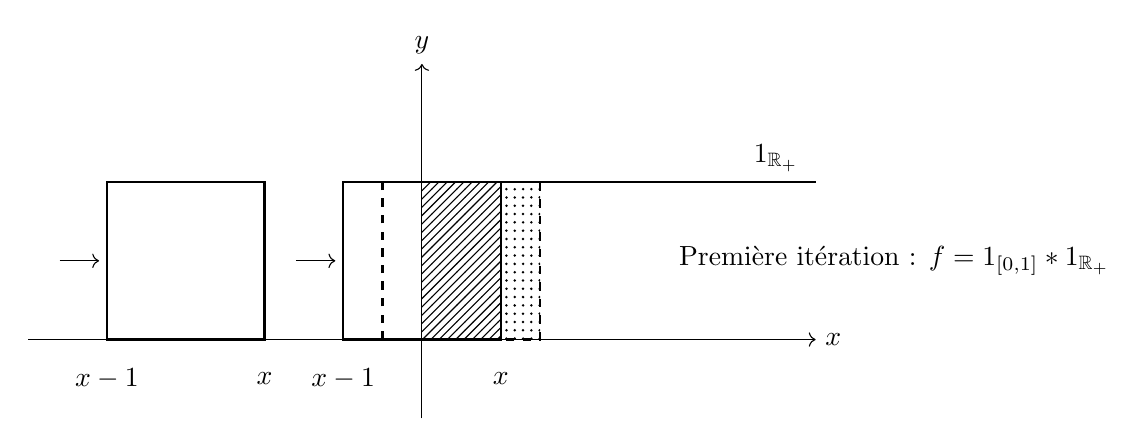
\begin{tikzpicture}
      % Axes
      \draw[->] (-5, 0) -- (5, 0) node[anchor=west] {$x$};
      \draw[->] (0, -1) -- (0, 3.5) node[anchor=south] {$y$};
   
      % Rectangles et flèches
      \draw[thick] (-4, 0) rectangle (-2, 2);
      \draw[->] (-4.6,1) -- (-4.1, 1);
   
      \draw[thick] (-1, 0) rectangle (1, 2);
      \draw[->] (-1.6, 1) -- (-1.1, 1);
   
      \draw[thick,dashed] (-0.5, 0) rectangle (1.5, 2);
   
      % Lignes de fonctions
      \draw[thick] (0, 2) -- (5,2);
   
      % Hachures
      %\fill[pattern=north east lines] (-4, 0) -- (-4, 2) -- (-2, 2) -- (-2,0) -- cycle;
      \fill[pattern=north east lines] (0, 0) -- (0, 2) -- (1, 2) -- (1,0) -- cycle;
      \fill[pattern=dots] (1, 0) -- (1, 2) -- (1.5, 2) -- (1.5,0) -- cycle;
   
      % Labels
      \node at (4.5, 2.3) {$1_{\R_+}$};
      \node at (-4, -0.5) {$x-1$};
      \node at (-2, -0.5) {$x$};
      \node at (-1, -0.5) {$x-1$};
      \node at (1, -0.5) {$x$};
   
      % Légende
      \node at (6,1) {Première itération : $f = 1_{[0,1]} \ast 1_{\R_+}$};
   \end{tikzpicture}

   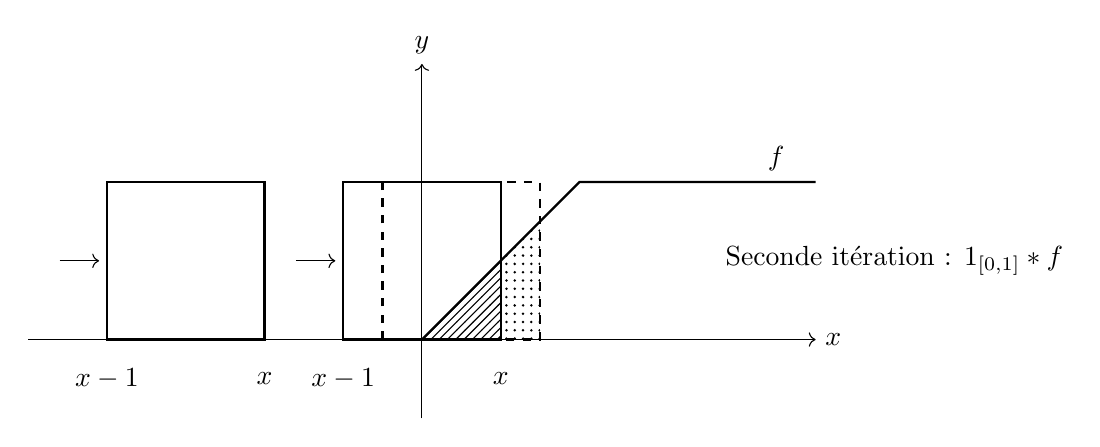
\begin{tikzpicture}
      % Axes
      \draw[->] (-5, 0) -- (5, 0) node[anchor=west] {$x$};
      \draw[->] (0, -1) -- (0, 3.5) node[anchor=south] {$y$};
   
      % Rectangles et flèches
      \draw[thick] (-4, 0) rectangle (-2, 2);
      \draw[->] (-4.6,1) -- (-4.1, 1);
   
      \draw[thick] (-1, 0) rectangle (1, 2);
      \draw[->] (-1.6, 1) -- (-1.1, 1);
   
      \draw[thick,dashed] (-0.5, 0) rectangle (1.5, 2);
   
      % Lignes de fonctions
      \draw[thick] (0,0) -- (2, 2) -- (5,2);
   
      % Hachures
      \fill[pattern=north east lines] (0,0) -- (1,1) -- (1,0) -- cycle ;
      \fill[pattern=dots] (1,0) -- (1,1) -- (1.5,1.5) -- (1.5,0) -- cycle ;
   
      % Labels
      \node at (4.5, 2.3) {$f$};
      \node at (-4, -0.5) {$x-1$};
      \node at (-2, -0.5) {$x$};
      \node at (-1, -0.5) {$x-1$};
      \node at (1, -0.5) {$x$};
   
      % Légende
      \node at (6,1) {Seconde itération : $1_{[0,1]} \ast f$};
   \end{tikzpicture}
\end{center}

\subsection*{\subsecstyle{Element neutre et suites régularisantes{:}}}
Soit \( f \in L^p \), on pourrait alors se demander si il existe un \textbf{élément neutre} pour cette opération. Et il se trouve qu'on montrera dans le chapitre suivant qu'il n'en existe pas. On souhaite alors approcher un tel élément neutre, en effet si il existait une suite de fonctions \( 1_n \) \textit{proche} de cet élément, ie telle que:
\[ 
   \vectNorm{1_n * f - f}_p \longrightarrow 0
\]
Alors la fonction \( 1_n * f \) serait proche de \( f \) mais gagnerait la régularité de \( 1_n \), cela motive la définition d'une \textbf{approximation de l'unité} comme étant une suite de fonctions positives intégrables \( (\phi_n)_n \) telles que pour tout \( \epsilon \) positif:
\[ 
   \begin{cases}
      \displaystyle \int_{\R^n} \phi_n(x) dx = 1\vspace{5pt} \\
      \displaystyle \int_{\mathcal{B}(0, \epsilon)^c} \phi_n(x) dx \longrightarrow 0
   \end{cases} 
\]
\uline{Exemple:} Une suite de fonctions portes de longueurs \( 1/n \) et de hauteurs \( n \) vérifient bien ces hypothèses, ce sont donc des approximations de l'unité.\<

Si de plus les \( (phi_n)_n \) sont lisses, on l'appelera alors \textbf{suite régularisante}, et si on a \( f \) une fonction d'intégrale 1, on peut construire une suite régularisante (si \( f \) est lisse) en posant (pour \( n \) la dimension de l'espace):
\[ 
   \phi_k(x) = k^n f(kx)
\]
Finalement étant muni de cette construction, on peut alors montrer qu'une telle suite régularisante vérifie bien la propriété asymptotique initiale de cette section, et approxime donc bien un élément neutre pour la convolution.
\chapter*{\chapterstyle{XI --- Transformée de Fourier}} % A REFAIRE
On se place dans l'espace mesuré\footnote[1]{Elle se définit en toute généralité dans \( \R^n \) en remplaçant \( \xi x \) par \( \xi \cdot x \), mais on choisit ici de simplifier l'exposition.} \( (\R, \mathscr{B}, \mu) \), on notera \( \mathcal{C}_b \) l'ensemble des fonctions continues bornées, alors on définit \textbf{la transformée de Fourier} de \( f \) par la fonction:
\[ 
   \begin{aligned}
      \mathcal{F} : L^1 &\longrightarrow \mathcal{C}_b \\
      f &\longmapsto \hat{f}
   \end{aligned}
\]
Où \( \hat{f} \) est la fonction suivante:
\[ 
   \quad\quad\quad\quad\quad\quad\quad\begin{aligned}
      \hat{f} : \R &\longrightarrow \C \\
      \xi &\longmapsto \int_{ \R} e^{-2\pi i\xi x} f(x)dx
   \end{aligned}
\]
L'intérêt de cette transformation est d'exploiter les symétries circulaires des fonctions \(x \mapsto e^{-2\pi i\xi x} \) pour détecter le spectre fréquentiel d'une fonction \( f \) donnée, qu'on appelera souvent \textbf{signal} dans ce contexte. On dira alors que \( f \) est dans le \textbf{domaine temporel} et \( \hat{f} \) dans le \textbf{domaine fréquentiel}. Voici une représentation heuristique de la transformation:

\begin{center}
   \definecolor{lightgray}{rgb}{0.8, 0.8, 0.8} %grid of coordinate system, axes
   \definecolor{midgray}{rgb}{0.6, 0.6, 0.6} %layer of border
   \definecolor{darkgray}{rgb}{0.4, 0.4, 0.4} %curves, fill under curve
   \vspace{5pt}
   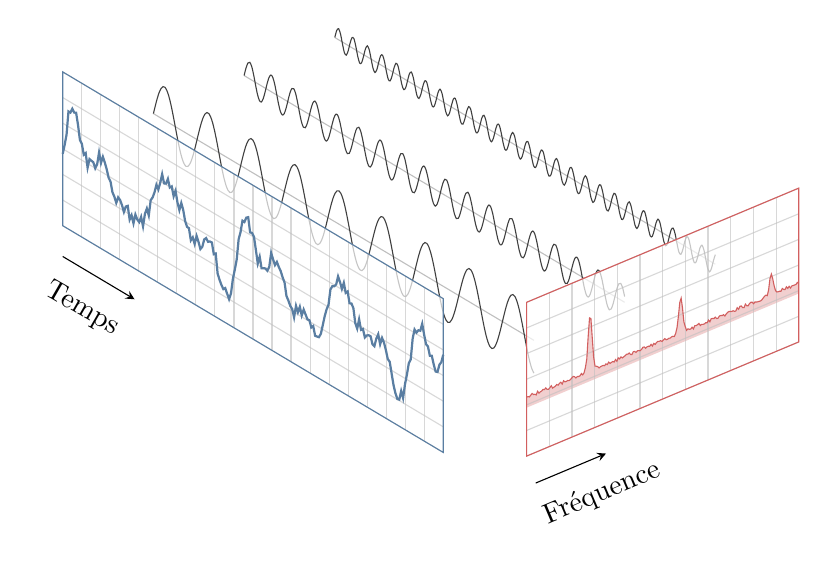
\begin{tikzpicture}[scale=1.7, every node/.style={scale=1.7}] %create tikz picture
      \pgfplotsset{compat=1.8}
   
       \begin{axis}[ %create 3d plot within tikz
           set layers=standard, %use predefined layers
           view={50}{30}, %perspective adjustment
           domain=0:10, %plot limit in time direction
           samples y=1, %samples for frequency direction
           unit vector ratio*=1 2 1, %rescale unit vectors
           hide axis, %do not plot axes
           xtick=\empty, ytick=\empty, ztick=\empty, %no ticks on coordinate axes
           clip=false %let me plot outside the coordinate system
       ]
           %limit variables
           \def\xmax{100} %limits for curves and layers
           \def\xmin{0}
           \def\ymax{35}
           \def\ymin{5}
           \def\zmax{25}
           \def\zmin{-5}
           \def\xlayer{110} %frequency layer
           \def\sumcurve{0} %sum curve of time signal
   
           %frequency curves
           \pgfplotsinvokeforeach{1,2,3}{ %for each frequency component
               \draw [on layer=background, lightgray] (axis cs:0,#1,0) -- (axis cs:10,#1,0); %axes
               \addplot3 [on layer=main, darkgray, smooth, samples=200] (x,#1,{1.3*sin(2*#1*x*(157))/(#1*2)}); %plot curves (curves are somewhat arbitrary)
   
               \xdef\sumcurve{\sumcurve + sin(#1*x*(157))/(#1*2)} %add current curve to sumcurve
           }
   
           %transparent layers
           \fill[white,opacity=0.7] (\xmin,0,\zmin) -- (\xmin,0,\zmax) -- (\xmax,0,\zmax) -- (\xmax,0,\zmin) -- cycle; %transparent layer in time space
           \fill[white,opacity=0.7] (\xlayer,\ymin,\zmin) -- (\xlayer,\ymin,\zmax) -- (\xlayer,\ymax,\zmax) -- (\xlayer,\ymax,\zmin) -- cycle; % transparent layer for frequency space
   
           %grid lines
           \pgfplotsinvokeforeach{\xmin,\xmin+5,...,\xmax}{ %create horizontal grid lines (time layer)
               \draw[lightgray,opacity=0.6] (#1,0,\zmin) -- (#1,0,\zmax);
           }
           \pgfplotsinvokeforeach{\ymin,\ymin+2.5,...,\ymax}{ %create horizontal grid lines (frequency layer)
               \draw[lightgray,opacity=0.6] (\xlayer,#1,\zmin) -- (\xlayer,#1,\zmax);
           }
           \pgfplotsinvokeforeach{\zmin,\zmin+5,...,\zmax}{ %create vertical grid lines (both layers)
               \draw[lightgray,opacity=0.6] (\xmin,0,#1) -- (\xmax,0,#1);
               \draw[lightgray,opacity=0.6] (\xlayer,\ymin,#1) -- (\xlayer,\ymax,#1);
           }
   
           %borders layer
           \draw[DarkBlue3] (\xmin,0,\zmin) -- (\xmin,0,\zmax) -- (\xmax,0,\zmax) -- (\xmax,0,\zmin) -- cycle; %time space layer border line
           \draw[BrightRed1] (\xlayer,\ymin,\zmin) -- (\xlayer,\ymin,\zmax) -- (\xlayer,\ymax,\zmax) -- (\xlayer,\ymax,\zmin) -- cycle; %frequency space layer border line
   
           %sum curve
           \addplot3 [DarkBlue3, thick, samples=200] (x,0,{\sumcurve+rand/7+0.2*sin(x*400)}); %sum curve time space with added random noise
   
           % frequency curve
           \addplot3 [BrightRed1, name path=f,samples=200,domain=0.5:3.5] (11,x,{rand/30+2*sin((x-0.7)*180)^200*e^(-x/2)-0.3}); %experimentally modified curve with noise
   
           %create fill under curve
           \addplot3 [name path=ax,draw=none,samples=2,domain=0.5:3.5] (11,x,-0.5); %create fill axis
           \addplot3 [BrightRed1] fill between [of=f and ax]; %create fill between curve and axis
   
           %create coordinate axis
           \draw[-{stealth}] (\xmin,0,\zmin-6) -- (\xmax/5.3,0,\zmin-6); %time axis
           \draw[-{stealth}] (\xlayer,\ymin+1,\zmin-6) -- (\xlayer,\ymin+\ymax/4,\zmin-6); %frequency axis
   
           %axis labels
           \node[scale=0.6, rotate=-30] at (5,0,-19) {Temps}; %axis time space
           \node[scale=0.6, rotate=23] at (100,17.5,-26) {Fréquence}; %axis frequency space
       \end{axis}
   \end{tikzpicture}
\end{center}

\subsection*{\subsecstyle{Lemme de Riemann-Lebesgue {:}}}
Une résultat fondamental de cette transformation est la suivante:
\begin{center}
   \textbf{La transformée de Fourier d'une fonction est un fonction qui tends vers zéro à l'infini.}
\end{center}
On notera \( \mathcal{C}_0 \) les fonctions qui tendent vers 0 à l'infini.

\pagebreak
\subsection*{\subsecstyle{Propriétés {:}}}
On peut alors montrer plusieurs propriétés de cette transformation, en notant \( P(x) =  2i\pi x\), on a:
\begin{itemize}
   \item C'est une \textbf{opérateur linéaire continu} pour la norme infini sur \(  \mathcal{C}_0 \).
   \item C'est une \textbf{opérateur autoadjoint} pour le produit scalaire de \( L^2 \).
   \item C'est une \textbf{opérateur injectif}.
   \item Elle transforme \textbf{les produits par des polynômes en dérivées}, ie si \( f \in L^1\), alors:
   \[ 
      \mathcal{F}(Pf) = -(\mathcal{F}(f))'
   \]
   \item Elle transforme \textbf{les dérivées en produit par des polynômes}, ie si \( f \in L^1 \cap \mathcal{C}^1 \) et que \( f' \in L^1 \), alors:
   \[ 
      \mathcal{F}(f') = P\mathcal{F}(f) 
   \]
\end{itemize}
La dernière propriétés est trés puissante dans l'étude des équations différentielles, en effet si on considère une fonction lisse \( y \) vérifiant par exemple:
\[ 
   y''(t) + y'(t) =  f(t)
\]
Alors on pourrait penser à appliquer la transformation de Fourier à cette équation, et ainsi transformer l'équation différentielle en équation algébrique:
\[ 
   P^2(t)\hat{y}(t) + P(t)\hat{y}(t) = \hat{f}(t) 
\]
Et finalement obtenir
\[ 
   \hat{y}(t) = \frac{\hat{f}(t)}{P^2(t) + P(t)}
\]
Alors si on arrivait à \textbf{inverser} la transformation de Fourier, on pourrait reconstituer \( y \) et conclure. On cherche donc à trouver une partie de \( \mathcal{C}_0 \) telle que la transformation restreinte soit surjective.

\subsection*{\subsecstyle{Inverse {:}}}
La transformation est injective, donc en particulier si on restreint \( \mathcal{F} \) à son image \( \mathcal{F}(L^1) \), alors on obtient une \textbf{bijection}, mais on préfère se restreindre à la partie \( \mathscr{A} := L^1 \cap \mathcal{F}(L^1) \) des fonctions dites \textbf{Fourier-intégrables}, alors on peut montrer que son inverse est donné par la formule:
\[ 
   \mathcal{F}^{-1}(f) = \int_\R e^{2 \pi i \xi x} \hat{f}(x) dx
\]

\subsection*{\subsecstyle{Propriétés de l'ensemble des fonctions Fourier-intégrables {:}}}
On peut alors montrer que \( \mathscr{A} \subseteq L^1 \cap \mathcal{C}_0 \) donc \( \mathscr{A} \subseteq L^1 \cap L^\infty \subseteq L^p \) et en outre, \( \mathscr{A} \) est \textbf{stable par produit simple et de convolution.} En outre on a la propriété suivant entre le produit simple et le produit de convolution:
\[ 
   \hat{fg} = \hat{f}*\hat{g} 
\]

\subsection*{\subsecstyle{Egalité de Plancherel{:}}}
En particulier si deux fonctions \( f, g \in \mathscr{A} \), on a alors \textbf{l'égalité de Plancherel}:
\[ 
   \dotproduct{f}{g} =  \dotproduct{\hat{f}}{\hat{g}}
\]
En d'autres termes, la transformée de Fourier est une \textbf{isométrie} de \( \mathscr{A} \) sur lui même pour la norme 2. On peut alors montrer que la transformée de Fourier est \textbf{continue} sur \( \mathscr{A} \) et en utilisant le \textbf{théorème de pronlongement uniforme}, ainsi que le fait que \( L^1 \cap L^2 \) est dense dans \( L^2 \), on peut alors montrer qu'il existe un unique prolongement de Fourier sur tout \( L^2 \) et c'est une isométrie bijective.
\chapter*{\chapterstyle{XI --- Séries de Fourier}} % A REFAIRE
Dans ce chapitre, on cherche à repliquer le concept de la transformée de Fourier dans le cadre des signaux \textbf{périodiques}. En d'autres termes de décomposer un tel signal en somme de signaux élémentaires. Dans toute la suite, on étudiera sans perte de généralité les fonctions \( 1 \)-périodiques, celles ci s'identifient alors à des fonctions sur le cercle \( \R/\Z \), ou encore aux fonctions définies sur le segment \( \icc{0}{1} \).

\subsection*{\subsecstyle{Famille de Fourier {:}}}
L'idée principale, à nouveau, est de considérer la famille particulières dite \textbf{famille de Fourier} suivante:
\[ 
   \mathcal{F} := \left(e^{2i\pi kx}\right)_{k \in \Z} = (e_k)_{k \in \Z}
\]
On peut alors montrer que \( \mathcal{F} \) est une \textbf{base Hilbertienne} de l'espace des fonctions périodiques \( L^2(\icc{0}{1})\).
\subsection*{\subsecstyle{Coefficients de Fourier {:}}}
En particulier d'aprés la théorie hilbertienne, si \( f \in L^2(\icc{0}{1}) \), alors on appelle \textbf{coefficients de Fourier} de \( f \) et on note \( c_k(f) \) la famille de terme général \(\dotproduct{e_k}{f}\) et on a:
\begin{itemize}
   \item L'égalité de décomposition:
   \[ 
      f = \sum_{n \in \Z} \dotproduct{e_k}{f}e_k = \sum_{n \in \Z} c_k(f)e_k
   \]
   \item Le théorème de Pythagore:
   \[ 
      \vectNorm{f}^2 = \sum_{n \in \Z} \left|\dotproduct{e_k}{f}\right|^2 = \sum_{n \in \Z} \left|c_k(f)\right|^2
   \]
\end{itemize}
On appelle alors la série ci-dessus \textbf{série de Fourier} de \( f \).
\subsection*{\subsecstyle{Symmétrisation des coefficients {:}}}
Si on considère la série de Fourier d'une fonction, on peut écrire:
\begin{flalign*}
   f &= \sum_{k \in \Z} c_k(f)e_k\\
   &= c_0(f) + \sum_{n = 1}^\infty c_k(f)e^{2i \pi kx} + c_{-k}e^{-2i \pi kx} \shorteqnote{(Les termes de la somme sont appelés \( n \)-ième \textbf{harmoniques} de \( f \))}\\
   &= c_0(f) + \sum_{n = 1}^\infty (c_k(f) + c_{-k}(f))\cos(2 \pi kx) + (i(c_k(f) - c_{-k}(f)))\sin(2 \pi kx)\\
   &= c_0(f) + \sum_{n = 1}^\infty a_k(f)\cos(2 \pi kx) + b_k(f)\sin(2 \pi kx)
\end{flalign*}
Ainsi on peut aussi décomposer \( f \) dans la base \((\cos(2 \pi kx), \sin(2 \pi kx))_{k \in \N} \) et écrire \( f \) comme une \textbf{série trigonométrique}. Ceci simplifie alors grandement certains applications nécessitant de représenter la série par exemple. Les relations entre les coefficients étant par ce qui précéde:
\[ 
   \begin{cases}   
      \displaystyle
      a_k(f) = c_k(f) + c_{-k}(f) = 2 \int_0^1 \cos(2 \pi kx)f(x)dx\\
      \displaystyle
      b_k(f) = i(c_k{f} - c_{-k}(f)) = 2 \int_0^1 \sin(2 \pi kx)f(x)dx
   \end{cases}
\]
En outre ceci permet d'utiliser la parité de la fonction, en effet on a:
\begin{itemize}
   \item Si \( f \) est \textbf{paire}, on a \( \forall k \in \N^* \; ; \; b_k = 0 \)
   \item Si \( f \) est \textbf{impaire}, on a \( \forall k \in \N^* \; ; \; a_k = 0 \)
\end{itemize}
\subsection*{\subsecstyle{Transformée de Fourier périodique {:}}}
Néanmoins de manière générale, on étends cette définition au cas des fonctions \( f \in L^1( \icc{0}{1}) \) et on définit la transformée de Fourier périodique par:
\[
   \begin{aligned}
      \mathcal{F}: L^1( \icc{0}{1}) &\longrightarrow \ell^\infty(\Z)\\
      f &\longmapsto (c_k(f))_{k \in \Z}
   \end{aligned}
\]
On peut alors montrer les propriétés suivantes analogues à la transformée de Fourier non-périodique:
\begin{itemize}
   \item \textbf{Lemme de Riemann-Lebesgue:} La transformée de Fourier est une famille qui tends vers \( 0 \) aux infinis.
   \item \textbf{Injectivité:} La transformée de Fourier est une fonction injective.
   \item \textbf{Dérivations:} La transformée de Fourier transforme aussi les dérivées en produits par des polynômes de manière analogue au cas non-périodique, ie on a:
   \[ 
      \mathcal{F}(f') = (2i\pi k c_k(f))_{k \in \Z}
   \]
\end{itemize} 
\subsection*{\subsecstyle{Modes de convergence de la série de Fourier {:}}}
On appelle \textbf{somme partielle de Fourier} la somme:
\[ 
   S_n(f) = \sum_{k = -n}^n c_k(f)e_k 
\] 
Alors le cas où \( f \in L^2(\icc{0}{1}) \), on a égalité de décomposition dans \( L^2(\icc{0}{1} \) et donc plus précisément, la famille est sommable et donc pour l'énumération de cette somme partielle, on a:
\[ 
   \lim_{n \rightarrow \infty}\vectNorm{f - S_n(f)}_2 = 0
\]
Ceci nous dit alors que la somme partielle de Fourier convergence dans cet espace, donc presque partout, mais ne dit rien de sa convergence \textbf{ponctuelle ou uniforme}. Ces problèmes difficiles font l'objet des sections suivantes.

\subsection*{\subsecstyle{Convergence uniforme {:}}}
On définit \textbf{l'algèbre de Weiner} par l'ensemble suivant:
\[ 
   W(\icc{0}{1}) := \left\{ f \in L^1(\icc{0}{1}) \; ; \; \left(\vectNorm{c_k(f)e_k}_\infty\right)_{k \in \Z} = \left(|c_k(f)|\right)_{k \in \Z} \text{ est sommable.} \right\}  
\]
Alors si une fonction \( f \) appartient à cet ensemble, on peut montrer que la série de Fourier de celle-ci \textbf{converge uniformément}, et donc ponctuellement, et on a:
\[ 
   \lim_{n \rightarrow \infty}\vectNorm{f - S_n(f)}_\infty = 0
\]
On peut alors montrer une condition nécessaire à l'appartenance à \( W(\icc{0}{1}) \), en effet on a:
\[ 
   \mathcal{C}^0(\icc{0}{1}) \cap \mathcal{C}^1_{pm}(\icc{0}{1}) \subseteq W(\icc{0}{1})
\]
En particulier \( \mathcal{C}^1(\icc{0}{1}) \subseteq W(\icc{0}{1}) \) et les fonctions périodiques \( \mathcal{C}^1 \) admettent une série de Fourier uniformément convergente.

\subsection*{\subsecstyle{Convergence ponctuelle {:}}}
De manière encore plus générale, si \( f \in \mathcal{C}^1_{pm}( \icc{0}{1})\), alors on peut montrer le résultat suivant:
\[ 
   S_n(f) \longrightarrow \frac{f(x^+) + f(x^-)}{2} 
\]
Où \( f(x^+) \) et \(  f(x^-)  \) représentent la limite par valeurs supérieures et inférieures de \( f \) en chaque point.
   \pagebreak   

   \addcontentsline{toc}{chapter}{Probabilités} % 95%
   \chapter*{\chapterstyle{XII --- Espaces probabilisés}} % 75% Fini
\addcontentsline{toc}{section}{Espaces probabilisés}
Le domaine des probabilités chercher à modéliser des \textbf{expériences aléatoires} ie des expériences dont toutes les \textbf{issues} possibles sont connues à priori mais dont le résultat peut varier lorsqu'on la répète (lancer de dés, tirage dans une urne\ldots).\<

Le cadre de la théorie de la mesure, nous permet de formaliser la théorie axiomatique des probabilités, ainsi que les différents objets en jeu, en particulier, on considère un espace mesurable \( ( \Omega, \mathcal{A}) \) muni d'une mesure \( \mathbb{P} \) à valeurs dans \( \icc{0}{1} \) et telle que \( \mathbb{P}( \Omega) = 1 \). On apelle une telle mesure \textbf{loi de probabilité}.\<

Le triplet \( ( \Omega, \mathcal{A}, \mathbb{P}) \) est alors apellé \textbf{espace probabilisé}. Dans ce cadre l'ensemble \( \Omega \) des issues possibles de l'expérience est apellé \textbf{univers}, les parties mesurables sont apellées \textbf{évenements} et deux parties mesurables disjointes seront dites \textbf{incompatibles}.

\subsection*{\subsecstyle{Espace probabilisé discret et continu}}
La mesure de l'espace doit être égale à 1 donc en particulier, on doit avoir \( \int_ \Omega d \mathbb{P} = 1 \), ceci étant dit, on peut alors distinguer deux grands cas d'espaces probabilisés:
\begin{itemize}
   \item Le cas où les parties non-négligeables de \( \Omega \) sont \textbf{dénombrables}, alors par applications de la relation de Chasles et l'invisibilité des parties négligeables, on obtient que:
   \[ 
      \int_\Omega d \mathbb{P} = \int_{\bigcup x_n} d \mathbb{P} = \sum_n \mathbb{P}(x_n)
   \]
   On remarque alors que la loi de probabilité est entièrement déterminée par la probabilité \textbf{d'évenements élémentaires} d'une certaine famille \( (x_n) \) dont la série vaut 1. On appele cette famille \textbf{distribution} de \( \mathbb{P} \) et de tels espaces \textbf{espaces probabilisés discrets}.
   \item Le cas où elles ne le sont pas et que \( \Omega \subseteq \R^n \), alors il est toujours possible de définir la \textbf{fonction de répartition} de la mesure de probabilité par la fonction suivante qui caractérise la loi:
   \[ 
      F : x \longrightarrow \mathbb{P}(\ioc{-\infty}{x})
   \]
   Si de plus les non-boréliens sont négligeables pour \( \mathbb{P} \) (on dit aussi que \( \mathbb{P} \) est \textbf{absolument continue} par rapport à la mesure de Lebesgue) alors on peut montrer que \( \mathbb{P} \) admet une densité, c'est à dire une fonction intégrable \( f \) dont l'intégrale vaut 1 et qui caractérise alors la probabilité:
   \[ 
      \mathbb{P}(A) = \int_A f(x)dx 
   \]
   On dira alors que ces lois sont des \textbf{lois à densité}. Si la dernière condition n'est pas vérifiée, on dira alors que la loi est \textbf{mixte ou singulière}.
\end{itemize}
\subsection*{\subsecstyle{Espace probabilisé produit}}
Si on se donne une famille de \( n \) espaces probabilisés \( ( \Omega_i, \mathscr{A}_i, \mathbb{P}_i) \), on peut alors conformément à la théorie de la mesure définir l'espace produit \( ( \prod \Omega_i, \mathscr{A}_\otimes, \mathbb{P}_\otimes ) \) avec la tribu et la loi produit. Dans tout la suite on considère simplement le cas \( n=2 \) pour simplifier.

Selon le cas discret ou a densité, on a alors que la loi est caractérisée par:
\begin{itemize}
   \item \textbf{Cas dénombrable:}
   \[
      \mathbb{P}_\otimes(A) = \sum_{\N \times \N} \mathbb{P}_\otimes(x_n, y_m)
   \]
   \item \textbf{Cas absolument continu:}
   \[
      \mathbb{P}_\otimes(A) = \int_{\Omega_1 \times \Omega_2} f(x, y) d\mathbb{P}_\otimes
   \]
\end{itemize}
\pagebreak
\subsection*{\subsecstyle{Lois marginales}}
Sachant la loi produit \( \mathbb{P} \), une question intéressante est alors de determiner les lois \textbf{marginales} des espaces composantes, on montre alors qu'on a:
\begin{itemize}
   \item \textbf{Dans le cas dénombrable:}
   \[
      \mathbb{P}_1(\{k\}) = \sum_{\N} \mathbb{P}(\{k\}, y_m)
   \]
   \item \textbf{Dans le cas absolument continu:}
   \[
      f_1(x) = \int_{\Omega_1} f(x, y) dy
   \]
\end{itemize}
Malheureusement on peut montrer que la donnée des lois marginales ne caractérise pas la loi produit, en effet les lois marginales dans le cas fini par exemple correspondent aux sommes des lignes ou colonnes du tableau des probabilités et deux sommes peuvent être égales sans que les valeurs individuelles soient toutes égales.
\subsection*{\subsecstyle{Exemples}}
Plusieurs exemples de différentes natures:
\begin{itemize}
   \item \textbf{Discret fini:} Si on cherche à modéliser 3 tirages successifs à pile ou face avec une pièce non truquée, on peut modéliser cette expérience par l'espace probabilisé suivant:
   \[ 
      \left(\left\{ (r_1, r_2, r_3) \; ; \; (r_i) \in \{P, F\}\right\}, \mathcal{P}( \Omega), \mathbb{P}(A) = \frac{|A|}{| \Omega|} \right)
   \]
   \item  \textbf{Discret infini:} Si on cherche à modéliser le nombres de visiteurs qui se présentent dans un musée, on peut alors modéliser ce phénomène par un espace probabilisé dénombrable et une probabilité rapidement décroissante, ie on pose par exemple:
   \[ 
      \left(\N, \mathcal{P}( \N), \mathbb{P}(\{n\}) = \frac{1}{2^{n+1}  } \right)
   \]
   Alors ceci est bien un espace probabilisé discret infini.
   \item \textbf{Absolument continu:} Si on cherche à modéliser un tir de fléchette sur le disque unité \( D \subseteq \R^2 \)où la probabilité suit une densité uniforme, alors on peut poser:
   \[ 
      \left( D, \mathcal{B}(D), \mathbb{P}(D) = \frac{1}{ \pi}\int_A d \mu = \frac{ \mu(A)}{ \pi}\right)
   \]
   \item \textbf{Mixte:} Si on cherche à modéliser une loterie où l'on tire un nombre de \( \icc{0}{10} \) avec \( \mathbb{P}(\{0\}) = 0.1 \) qui correspond au jackpot et densité uniforme pour le reste des nombres. Alors on a naturellement une structure d'espace probabilisé mixte.
   \item \textbf{Espace produit:} Si on cherche à modéliser le choix uniforme d'un point dans \( \inticc{1}{n}^2 \), on modèlise ceci par l'espace produit:
   \[ 
      (\inticc{1}{n}^2, \mathcal{P}(\inticc{1}{n}^2), \mathbb{P}(\{(k, l)\}) = \frac{1}{n^2}) 
   \]
   Alors les distributions marginales sont facilement \( \mathbb{P}_1(\{k\}) = \mathbb{P}_2(\{k\}) = \frac{1}{n} \), on a en fait le tableau des probabilités décrit par la matrice de taille \( n \) suivante:
   \[ 
      \begin{pmatrix}                   
         \frac{1}{n^2} & \ldots & \frac{1}{n^2}\\
         \vdots & \ddots & \vdots\\
         \frac{1}{n^2} & \ldots & \frac{1}{n^2}
      \end{pmatrix}
   \]
   Les colonnes (resp. lignes) correspondant aux probabilités \( \mathbb{P}_1(\{k\}) \) (resp. \( \mathbb{P}_2(\{k\}) \))
\end{itemize}
\chapter*{\chapterstyle{XII --- Probabilités conditionnelles}} % 75% Fini
Lorsque l'on dispose d'informations sur le résultat d'une expérience donnée, il est possible d'affiner nos
prédictions. \+
Soit \(X\) un évenement qui n'est pas négligeable, alors on définit l'application:
\[
   \begin{aligned}
      \mathbb{P}( \cdot | X): \Pow(\Omega) &\longrightarrow \icc{0}{1}\\
      A &\longmapsto \frac{\mathbb{P}(A \cap X)}{\mathbb{P}(X)}
   \end{aligned}
\]
On peut montrer que c'est une mesure de probabilité sur \(\Omega\) et on l'appelle \textbf{probabilité de A sachant X}. De la symétrie de l'intersection on peut alors en déduire la \textbf{formule de Bayes} qui permet alors \textbf{d'inverser le conditionnement}:
\[
   \mathbb{P}(A | B) = \frac{\mathbb{P}(A) \mathbb{P}(B | A)}{\mathbb{P}(B)}
\]
\subsection*{\subsecstyle{Formule des probabilités composées}}
On en déduit directement la \textbf{formule des probabilités composées}:
\[
      \mathbb{P}(A \cap B) = \mathbb{P}(A)\mathbb{P}(B | A) = \mathbb{P}(B)\mathbb{P}(A | B)
\]

Qui se généralise pour une famille finie d'évenements \((A_n)_{n \in I}\) d'intersection non nulle:
\[
   \mathbb{P}(A_1 \cap \ldots \cap A_n) = \mathbb{P}(A_1)\mathbb{P}_{A_1}(A_2)\mathbb{P}_{A_1\cap A_2}(A_3)\ldots\mathbb{P}_{A_1\cap \ldots \cap A_{n-1}}(A_n)
\]
\subsection*{\subsecstyle{Formule des probabilités totales}}
On considère une partition \((A_n)_n\) de \( \Omega \) en évenements disjoints (on appelle une telle partition \textbf{systême complet d'évenements}), alors on peut montrer la \textbf{formule des probabilités totales}:
\[
   \mathbb{P}(B) = \sum_{k=1}^{n} \mathbb{P}(A_k) \mathbb{P}_{A_k}(B)
\]
\subsection*{\subsecstyle{Indépendance}}
On dit que deux évenements \(A, B\) sont \textbf{indépendants} si et seulement si la donnée de la réalisation d'un des évenements n'influence pas l'autre, ie:
\[ 
   \mathbb{P}(A | B) = \mathbb{P}(A)  
\]
Ou encore par la formule conditionelle:
\[
      \mathbb{P}(A \cap B) = \mathbb{P}(A)\mathbb{P}(B)
\]
Si deux évenements sont indépendants, alors n'importe quelle paire de \(A, B, \overline{A}, \overline{B}\) est indépendante.
\chapter*{\chapterstyle{XII --- Lois usuelles}} % 75% Fini
Dans ce chapitre, on énumère les lois usuelles en probabilité et leurs cas d'utilisation. Comme vu précédement, on distingue le cas discret et absolument continu. Dans tout la suite on considère un espace probabilisé \( ( \Omega, \mathscr{A}, \mathbb{P}) \).

\subsection*{\subsecstyle{Lois discretes usuelles}}
On appelle \textbf{épreuve de Bernoulli} est une expérience aléatoire qui n'a que deux issues, usuellement nommées \textbf{succés et échec}.\<

On dit que la loi est \textbf{uniforme} si on a la distribution:
\[
   \forall A \in \mathscr{A} \; ; \; \mathbb{P}(A) = \frac{|A|}{|E|}  
\]
On dit que la loi est \textbf{binomiale} de paramêtres \(n, p\) si \( \Omega = \{1, \ldots, n\}\) et si on a la distribution:
\[
   \forall k \leq n \; ; \; \mathbb{P}(\{k\}) = \binom{n}{k} \; p^k(1-p)^{n-k}
\]
On dit que la loi est \textbf{géométrique} de paramêtre \( p \) si \(\Omega = \N^*\) et si on a la distribution:
\[
   \forall k \geq 1 \; ; \;  \mathbb{P}(\{k\}) = p(1 - p)^{k - 1}
\]
On dit que la loi est \textbf{hypergéométrique} de paramêtres \((p, n, N)\) si \(\Omega = \N^*\) et si on a la distribution:
\[
   \forall k \geq 1 \; ; \; \mathbb{P}(\{k\}) = \frac{\binom{pN}{k}\binom{(1-p)N}{n - k}}{\binom{N}{n}}
\]
On dit que la loi est \textbf{de Poisson} de paramêtres \( \lambda\) si \(\Omega = \N^*\) et si on a la distribution:
\[
   \forall k \geq 1 \; ; \; \mathbb{P}(\{k\}) = \frac{\lambda^k}{k!}e^{-\lambda}
\]\<

La \textbf{loi binomiale} est utilisée pour déterminer la probabilité d'obtenir exactement \(k\) succés aprés \(n\) itérations d'une épreuve de Bernoulli. \+
La \textbf{loi géométrique} est utilisée pour déterminer la probabilité d'un temps d'attente \( k \) avant le le premier succés d'une épreuve de Bernoulli.\+
La \textbf{loi hypergéométrique} est utilisée pour déterminer la probabilité d'obtenir \(k\) succés aprés \(n\) itérations d'une épreuve de tirage sans remise dans une urne contenant \(N\) boules, dont \(pN\) boules gagantes, et \((1-p)N\) boules perdantes, avec la contrainte que \(pN\) soit un entier.\+
La \textbf{loi de Poisson} est utilisée pour déterminer le nombre d'événements se produisant dans un intervalle de temps fixé, si ces événements se produisent avec une fréquence moyenne connue, et indépendamment du temps écoulé depuis l'événement précédent\footnote[1]{C'est une loi qui s'obtient asymptotiquement à partir d'une loi binomiale de paramêtres \(T, \frac{\lambda}{T}\) en faisant tendre \(T\) vers l'infini.}.

\pagebreak
\subsection*{\subsecstyle{Lois à densité usuelles}}

On dit que la loi est \textbf{uniforme} si sa densité \(f\) est constante sur un intervalle \(\icc{a}{b}\) et nulle en dehors.\+
On dit que la loi est \textbf{exponentielle} de paramètre \(\lambda\) si on a la densité:
\[
   f(x) = \lambda\exp{(-\lambda x)} \; ; \; x \geq 0  
\]
On dit que la loi est \textbf{normale} dee paramêtres\footnote[1]{Ces paramêtres correspondent alors à l'éspérance et l'écart type de la loi.} \(\mu, \sigma\) si on a la densité:
\[
   f(x) = \frac{1}{\sigma\sqrt{2\pi}} \exp{\left(-\frac{(x - \mu)^2}{2\sigma^2}\right)}
\]

La \textbf{loi exponentielle} est utilisée pour modéliser le temps d'attente d'un phénomène sans mémoire, en particulier, c'est l'analogue continue de la loi géométrique\footnote[2]{Elle s'obtient asymptotiquement à partir d'une loi géométrique de paramètre \(\lambda T\) en faisant tendre \(T\) vers 0.}. \+
La \textbf{loi normale} est fondamentale en probabilités du fait de son omniprésence dans les sciences expérimentales, en effet, un théorème fondamental montrera que la somme d'une suite de variables aléatoires (comprendre expériences) convergera vers une certaine loi normale. Elle est donc d'importance capitale en statistiques.\+
\chapter*{\chapterstyle{XII --- Variables aléatoires}} % 95% Fini
\addcontentsline{toc}{section}{Variables aléatoires}
Trés souvent, il se trouve que l'espace probabilisé de l'expérience est inconnu, trop grand ou trop complexe, on considérera alors simplement son existence et on étudiera celui ci via des fonctions définies sur cet espace, appelées \textbf{variables aléatoires}. Ces fonctions induiront un nouvel espace probabilisé correspondant à notre expérience précise (souvent un espace probabilisé numérique). \<

On considère alors souvent \( ( \Omega, \mathscr{A}, \mathbb{P}) \) comme un espace probabilisé abstrait et on l'oublie même complétement trés souvent. Par exemple:
\begin{itemize}
   \item On considère une expérience aléatoire qui tire au hasard un gateau dans une chaîne de fabrication, on peut alors définir une variable aléatoire sur l'espace probabilisé naturellement défini qui à chaque évenement associe le volume du gateau, son taux de sucre, le nombre de raisins secs ... Et faire alors des suppositions sur la loi de ces variables aléatoires par exemple on pourra supposer que le taux de sucre d'un gateau choisi au hasard suit une loi normale.
   \item Si on considère un groupe de \( N \) personnes vivant un épisode épidémique, alors il est trés compliqué de modéliser l'état épidémique du groupe à un instant donné du fait des différentes intéractions et dépendances, on préfère alors éudier des espaces probabilisés plus simples induits par des variables aléatoires comme le nombre de personnes infectées, le temps mis par l'épidémie pour atteindre une certaine taille etc ..
\end{itemize}
\subsection*{\subsecstyle{Définition}}
On dira que \( X \) est une \textbf{variable aléatoire} de \( ( \Omega_1, \mathscr{A}, \mathbb{P}) \) vers un espace mesurable \( ( \Omega_2, \mathscr{B}) \) si et seulement si c'est une \textbf{fonction mesurable} sur cet espace. Elle définit alors une loi naturelle sur \( \Omega_2 \) définie par la \textbf{mesure image}:
\[
   \begin{aligned}
      \mathbb{P}_X: \mathscr{B} &\longrightarrow \icc{0}{1}\\
      B &\longmapsto \mathbb{P}(X^{-1}(B))
   \end{aligned}
\]
On note alors plus simplement \( \mathbb{P}_X(B) = \mathbb{P}(X \in B) \). Trés souvent, on considérera \( (\R^n, \mathcal{B}( \R^n)) \) comme espace d'arrivée et donc la variable aléatoire sera dite \textbf{réelle} et définira une loi sur les boréliens.
\subsection*{\subsecstyle{Cas réel}}
Dans le cas de variables aléatoires \textbf{réelles} on peut aussi créer une notation qui s'applique si \(B\) est un intervalle et on a:
\[
   X^{-1}\bigl(\ioo{a}{b}\bigl) = \Bigl\{ \omega \in \Omega \; ; \;  a < X(\omega) < b\Bigl\} \notationEq (a < X < b)
\]
\subsection*{\subsecstyle{Propriétés}}
La famille \(((X = a))_{a \in X(\Omega)}\) est un \textbf{système complet d'évenements}, en effet car si on considère une issue \(\omega \in \Omega\), on a:
\[
   \begin{cases}
      X(\omega) = x \implies \omega \in (X = x)\\  
      X(\omega) \neq x \implies \omega \notin (X = x)   
   \end{cases} 
\]
\begin{center}
   \textit{On peut donc partitionner les éléments de \(\Omega\) selon leur image par \(X\)}
\end{center}
On peut aussi noter que si \(f\) est une application mesurable, alors \(f \circ X\) \textbf{est une variable aléatoire} sur les espaces correspondants.
\pagebreak
\subsection*{\subsecstyle{Indépendance}}
On dira alors que deux variables aléatoires \(X, Y\) sont indépendantes si et seulement si pour tout couple \(x, y\), les évenements correspondants sont indépendants:
\[
   \mathbb{P}(X = x \cap Y = y) = \mathbb{P}(X = x)\mathbb{P}(Y = y)  
\]
Par ailleurs, si \(X, Y\) sont deux variables aléatoires, il existe une mesure de la dépendance (corrélation) de deux variables aléatoires appellée \textbf{covariance} définie dans la dernière partie.
\subsection*{\subsecstyle{Cas des vecteurs aléatoires}}
Dans le cas où la variable aléatoire \( X = (X_1, \ldots, X_n) \) est à valeurs dans \( \R^n \), alors elle définit une loi produit (appelée dans ce cadre \textbf{loi conjointe} de \( X \)) sur les boréliens et on l'appelle \textbf{vecteur aléatoire}. En particulier les lois marginales sont alors les lois des variables composantes \( X_i \). Par exemple si on prends un vecteur aléatoire choisissant uniformément un point dans \( \inticc{1}{n}^2 \), alors on a que:
\[ 
   \mathbb{P}(X = (k, l)) = \frac{1}{n^2} 
\]
Et les loi marginales sont données par:
\[ 
   \mathbb{P}(X_1 = k) = \sum_{i=1}^n \mathbb{P}(X = (k, i))  
\]
On retrouve alors les même lois marginales que dans l'exemple analogue sans variable aléatoire, en particulier les lois conjointe et marginales sont exactement les lois produits et marginales sur \(\R \times \R\).   
\subsection*{\subsecstyle{Intégrabilité et formule de transfert}}
On se donne une variable aléatoire réelle intégrable par rapport à la mesure \( \mathbb{P} \) ie telle que:
\[ 
   \int_\Omega X( \omega)d \mathbb{P} < \infty 
\] 
Alors on peut montrer l'identité suivante par les propriétés de la mesure image \( d \mathbb{P}_X \):
\[ 
   \int_\Omega X( \omega) d \mathbb{P} = \int_{\R} xd \mathbb{P}_X
\]
Et même plus généralement, on a le \textbf{théorème de transfert} pour tout fonction \( \phi \) telle qu'une des intégrale ait un sens:
\[ 
   \int_\Omega \phi(X( \omega)) d \mathbb{P} = \int_{\R} \phi(x)d \mathbb{P}_X
\]
Et les intégrales du membre de droite se calculent souvent facilement, par exemple dans les deux cas classiques:
\begin{itemize}
   \item \textbf{Cas dénombrable:} On a 
   \[ 
      \int_{\R} xd \mathbb{P}_X = \sum_\N \int_{y_n} xd \mathbb{P}_X = \sum_\N y_n \mathbb{P}(X = y_n)
   \]
   \item \textbf{Cas absolument continu:} On a 
   \[ 
      \int_{\R} xd \mathbb{P}_X = \int_{\R}xf(x)dx  
   \]
\end{itemize}
\chapter*{\chapterstyle{XII --- Indicateurs}} % 80% Fini
\addcontentsline{toc}{section}{Indicateurs}
Dans tout la suite, on considère \((\Omega, \Pow(\Omega), \mathbb{P})\) un espace probabilisé fini et \(X, Y\) deux variables aléatoires \textbf{intégrables} pour la mesure \( \mathbb{P} \). \<

On appelle \textbf{indicateur de position} un nombre réel permettant de situer les valeurs d'une série statistique, par exemple l'esperance et la médiane sont des indicateurs de position.\+

On appelle \textbf{indicateur de dispersion} un nombre réel permettant de mesurer la variabilité des valeurs d'une série statistique autour d'une valeur (généralement autour de la moyenne), par exemple la variance, l'écart-type ou l'écart interquartile sont des indicateurs de dispersion.

\subsection*{\subsecstyle{Esperance}}
L'espérance mathématique correspond à la moyenne théorique du résultat qu'on peut espérer avoir en répétant une expérience aléatoire un grand nombre de fois, c'est \textbf{la moyenne des valeurs de la variable aléatoire, pondérées par leur probabilités respectives}, ou c'est aussi le centre de masse de la densité, on définit alors celle ci par:
\[
   \expectancy{X} := \int_\Omega X d\mathbb{P}
\]

L'esperance prends alors la forme d'une somme pondérée dans le cas discret, ou d'une intégrale pondéree dans le cas absolument continue. Elle existe toujours dans le cas d'une variable aléatoire \textbf{finie} mais ce n'est pas le cas en général, et il faut alors étudier l'intégrabilité de la variable aléatoire. \<

L'espérance possède plusieurs propriétés remarquables, elle est \textbf{linéaire et croissante} et l'espérance d'une constante est cette constante.\+
Mais en général, l'espérance \textbf{n'est pas multiplicative}, c'est néanmoins le cas quand les deux variables aléatoires sont \textbf{indépendantes}.
\subsection*{\subsecstyle{Variables centrées}}
On rappelle qu'on a le théorème de transfert donc \(\expectancy{\phi(X)}\) existe si \( \phi(X) \) est intégrable. Aussi, on appelle \textbf{variable centrée} une variable aléatoire d'espérance nulle. On peut alors centrer une variable aléatoire par la translation \(X' = X - \expectancy{X}\).
\subsection*{\subsecstyle{Moments d'ordre k}}
On généralise cette définition et on définit le \textbf{moment d'ordre k} de la variable \( X \), si il existe par la quantité suivante:
\[ 
   m_k(X) = \expectancy{X^k} 
\]
On remarque alors que cette quantité existe si et seulement si \( X^k \) est intégrable. De manière générale, on comprends facilement qu'on a la propriété suivante (où la disjonction dépends de la discrétude ou non de \( X \)):
\[ 
   X \text{ admet un moment d'ordre \( k \)} \iff X \in L^k( \Omega) \text{ ou } \ell^k( \Omega)
\]
\subsection*{\subsecstyle{Variance}}
On manque alors d'informations sur les valeurs de \(X\), elles peuvent tout aussi bien rester toujours très
proches de \(\expectancy{X}\), ou s'en éloigner beaucoup, on a donc besoin de mesurer la distance moyenne entre \(X\) et \(\expectancy{X}\), qui serait alors \(\expectancy{| X - \expectancy{X} |}\).\pagebreak

Cette formule est techniquement impraticable du fait de la valeur absolue, on utile donc \textbf{la moyenne des carrés des distances} entre \(X\) et \(\expectancy{X}\), et on définit alors la variance:
\[ 
   \variance{X} := \expectancy{(X - \expectancy{X})^2} = \expectancy{X^2} - \expectancy{X}^2
\]


La deuxième expression apellée \textbf{formule de Koenig-Huygens} se déduit facilement de la première par les propriétés de l'espérance et on en déduit qu'une variable aléatoire admet une variance si et seulement si elle admet un moment d'ordre 2.

On voit directement que la variance est \textbf{positive} (ou nulle si \(X\) est constante presque partout). Elle vérifie aussi les propriétés suivantes:
\begin{itemize}
   \item \textbf{Invariante par translation} \( \variance{X + a} = \variance{X} \)
   \item \textbf{Quadratique}  \( \variance{ \lambda X} = \lambda^2\variance{X} \)
\end{itemize}
\subsection*{\subsecstyle{Ecart type}}
On peut alors définir \textbf{l'écart-type} de la variable \(X\) qui est défini par \(\sigma(X) = \sqrt{\variance{X}}\)\<

Enfin, on appelle \textbf{variable réduite} une variable aléatoire d'écart type \(1\) et on peut alors définir la \textbf{variable centrée réduite} associée à \(X\):
\[
   X^*= \frac{X - \expectancy{X}}{\sigma(X)}  
\]
\subsection*{\subsecstyle{Covariance}}
Dans le cas d'un couple aléatoire et contrairement à l'espérance, le concept de variance perds son sens. Plutôt que de chercher un écart par rapport à la moyenne, on va préférer chercher \textbf{un écart moyen entre les deux variables}\footnote[1]{On remarque que la variance n'est alors que la covariance de \(X\) avec elle-même. Aussi si les deux variables aléatoires sont indépendantes, dans ce cas l'espérance est multiplicative et on a \(\text{Cov}(X, Y) = 0\), la reciproque étant \textbf{fausse}.} qui se définit par:
\[
   \text{Cov}(X, Y) = \mathbb{E}\bigl[(X - \mathbb{E}(X))(Y - \mathbb{E}(Y))\bigl] = \mathbb{E}(XY) - \mathbb{E}(X)\mathbb{E}(Y) 
\]
Gràce à la covariance on peut aussi définir la variance d'une somme:
\[ 
   \variance{X + Y} =   \variance{X} + \variance{Y} +  2\text{Cov}(X, Y)
\]
La covariance de \( X, Y \) n'existe bien sûr que si \( X, Y \) et \( XY \) sont intégrables. 
\subsection*{\subsecstyle{Propriétés de la covariance}}
La covariance vérifie plusieurs propriétés intéressantes:
\begin{itemize}
   \item Si les deux variables aléatoires sont indépendantes, alors on a \(\text{Cov}(X, Y) = 0\), la reciproque étant \textbf{fausse}.
   \item Si \( X \) admet une variance alors on retrouve celle ci comme \( \text{Cov}(X, X) \)
\end{itemize}

On peut même montrer que la covariance est \textbf{bilinéaire, symétrique et positive}. Informellement c'est un \textit{``pseudo produit scalaire''} sur les variables aléatoires, néanmoins suffisament proche du produit scalaire pour avoir \textbf{l'inégalité de Cauchy-Schwartz}:
\begin{align*}
   |\text{Cov}(X, Y)| \leq \sigma(X)\sigma(Y)
\end{align*}
Plus précisément, considérons l'espace des variables aléatoires centrées réduites, alors c'est \textbf{un espace prehilbertien}, et la covariance définit son produit scalaire, l'écart type définit alors la \textbf{norme} associée et on peut définir le coefficient de corrélaition linéaire par:
\[
   \rho_{X, Y} = \frac{\text{Cov}(X, Y)}{\sigma(X)\sigma(Y)}
\]
Qui s'intérpréterait alors comme \textit{l'angle} entre les variable aléatoires.
\pagebreak
\subsection*{\subsecstyle{Espérance \& variances usuelles}}
Il est intéressant de considérer les différents indicateurs de position et de dispersion des lois usuelles\footnote[1]{Pour la loi uniforme on considère \(X\) à valeurs dans \(\inticc{1}{n}\)}

\begin{center}
   \renewcommand{\arraystretch}{2}
   \setlength{\tabcolsep}{18pt}
   
   \begin{tabular}{|c||c|c|}
      \hline
      Lois & \cellcolor{BrightBlue1!40} Espérance & \cellcolor{BrightBlue1!40} Variance \\ 
      \hline
      \cellcolor{BrightBlue1!40} \(X \sim \mathcal{U}(E)\) & \(\frac{n+1}{2}\) & \(\frac{n^2 - 1}{12}\) \\ 
      \hline
      \cellcolor{BrightBlue1!40} \(X \sim \mathcal{B}(n, p)\) & \(n\cdot p\) &  \(n\cdot p(1-p)\) \\ 
      \hline
      \cellcolor{BrightBlue1!40} \(X \sim \mathcal{G}(p)\) & \(\frac{1}{p}\) & \(\frac{1-p}{p^2}\) \\ 
      \hline
      \cellcolor{BrightBlue1!40} \(X \sim \mathcal{H}(p, n, N)\) & \(n\cdot p\) & \(n\cdot p(1-p)\frac{N - n}{N - 1}\) \\ 
      \hline
   \end{tabular}
\end{center}

\subsection*{\subsecstyle{Inégalités}}
On souhaite majorer la probabilité d'avoir des valeurs "extrèmes", ie éloignées de l'espérance, alors si \(X\) est une variable aléatoire positive presque partout et \(\alpha \in \R^{+*}\) on peut montrer \textbf{l'inégalité de Markov}:
\[
   \mathbb{P}(X \geq \alpha) \leq \frac{\expectancy{X}}{\alpha}
\]
Si la variable aléatoire admet une variance, on a alors \textbf{l'inégalité de Bienaymé-Tchebychev}:
\[
   \mathbb{P}(|X - \expectancy{X}| \geq \alpha) \leq \frac{\variance{X}}{\alpha^2}
\]
Cette dernière est un cas particulier de la première mais est en général \textit{plus fine} que la majoration donnée par l'inégalité de Markov.
\chapter*{\chapterstyle{XII --- Convergences Stochastiques}} % 25% Fini
\addcontentsline{toc}{section}{Convergences Stochastiques}
On peut alors tenter d'appliquer les résultat sur les espaces \( L^p \) à la théorie des probabilité, en particulier étudier des intégrales de variables aléatoires, des espérances, etc .. revient à étudier la finitude d'un norme dans \(L^p(\Omega)\) en particulier pour tout \( p \in \icc{1}{\infty} \), on en déduis que les normes \( p \) s'appliquent aux variables aléatoires, ie on a:
\[ 
   \begin{cases}
      \vectNorm{X}_p := \left(\int_\Omega |X|^p d \mathbb{P} \right)^{ \frac{1}{p}} = \left( \expectancy{|X|^p} \right)^{ \frac{1}{p}}\\
      \vectNorm{X}_\infty := \sup\text{ess} \{ |X| \}

   \end{cases}
\]
Où ici \( X \) est supposée à densité ou à distribution \( f(x) \).\<

Cette approche sera alors trés fructueuse, en effet par l'étude et la définition de différent \textit{modes de convergences} bien choisis sur des suites de variables aléatoires \( (X_n) \), on pourra alors démontrer les grands théorèmes probabilistes.
\subsection*{\subsecstyle{Convergence en loi}}
On dira que \(X_n\) \textbf{converge en loi} vers \(X\) si et seulement si pour tout \(x \in \R\), la loi de \( X_n \) est abitrairement proche de la loi de \( X \), ie si on a:
\[
   \mathbb{P}(X_n \leq x) \longrightarrow \mathbb{P}(X \leq x)
\]
On notera alors:
\[
   (X_n) \overset{\mathcal{L}}{\longrightarrow} X
\]
\subsection*{\subsecstyle{Convergence en probabilité}}
On dira que \(X_n\) \textbf{converge en probabilité} vers \(X\) si et seulement si pour tout \(\epsilon > 0\), la probabilité que \( (X_n)_n \) s'éloigne de \( X \) tends vers 0, ie si on a:
\[
   \mathbb{P}(|X_n - X| > \epsilon) \longrightarrow 0
\]
On notera alors:
\[
   (X_n) \overset{\mathcal{P}}{\longrightarrow} X
\]
\subsection*{\subsecstyle{Convergence presque partout}}
On dira que \(X_n\) \textbf{converge presque partout} vers \(X\) si et seulement si elle converge sauf sur un domaine de mesure nul, ie:
\[
   \mathbb{P}\left( \left\{ \omega \in \Omega \; ; \; \lim_{n \rightarrow +\infty} X_n(\omega) \neq X(\omega) \right\}\right) = 0
\]
On notera alors:
\[
   (X_n) \longrightarrow X \; p.p.
\]
\subsection*{\subsecstyle{Convergence $L^p$}}
On dira qu'une suite \( (X_n) \) converge en norme p vers une variable aléatoire \( X \) si et seulement si:
\[ 
   \lim_{n \rightarrow \infty} \vectNorm{X_n - X}_p = \lim_{n \rightarrow \infty} \left(\expectancy{|X_n - X|^p}\right)^{ \frac{1}{p}} =  0 
\]
\subsection*{\subsecstyle{Relations entre les convergences}}
On peut montrer les différentes implications suivantes:
\[ 
   \textbf{Convergence p.p.} \implies \textbf{ Convergence en probabilité } \implies \textbf{Convergence en loi}
\]
Et pour \( p > q \geq 1 \)
\[ 
   \textbf{Convergence }L^p \implies \textbf{Convergence } L^q \implies \textbf{Convergence en probabilité}
\]
\chapter*{\chapterstyle{XII --- Théorèmes limites}} % 25% Fini
\addcontentsline{toc}{section}{Théorèmes limites}

Munis de nos nouveaux outils et modes de convergences des suites de variables aléatoires, on peut alors énoncer et démontrer les grands théorèmes probabilistes.
\subsection*{\subsecstyle{Lois des grands nombres}}
On se donne une suite de variables aléatoires indépendantes et identiquement distribuées (communément noté iid) \((X_n)\) admettant une espérance \(\mu\), et on pose une variable aléatoire appellée \textbf{moyenne\footnote[1]{Elle correspond à la moyenne faite sur les réalisations d'une expérience par exemple.} empirique}:
\[
   \overline{X}_n = \frac{1}{n}\sum_{k=1}^{n}X_k   
\]
Alors on peut montrer la loi \textbf{faible} des grands nombre, ie:
\[
   \overline{X}_n \overset{\mathcal{P}}{\longrightarrow} \mu
\]
Pour les memes hypothèses que précédemment la loi \textbf{forte} des grands nombres nous assure une convergence plus forte, ie on a:
\[
   \overline{X}_n \overset{p.s.}{\longrightarrow} \mu
\]
\subsection*{\subsecstyle{Théorème central limite}}
On se donne une suite de variables aléatoires iid \((X_n)\) admettant une espérance \(\mu\) et un écart-type \(\sigma\) finis, alors on considère à nouveau la moyenne empirique:
\[
   \overline{X}_n = \frac{1}{n}\sum_{k=1}^{n}X_k   
\]
Mais cette fois on considère cette variable sous sa forme \textbf{centrée réduite}, qu'on notera \(\overline{X}_n^*\), alors le théorème central limite nous donne que:
\[
   \overline{X}_n^* \overset{\mathcal{L}}{\longrightarrow} \mathcal{N}(0, 1)
\]
   \pagebreak   
   
   \addcontentsline{toc}{chapter}{Statistiques} % A FAIRE
   \chapter*{\chapterstyle{XIII --- Introduction}} % A REFAIRE
\addcontentsline{toc}{section}{Introduction} 
   \pagebreak

   \addcontentsline{toc}{chapter}{Analyse Numérique} % 95%
   \chapter*{\chapterstyle{XIV --- Introduction}}
\addcontentsline{toc}{section}{Introduction}

L'analyse numérique est la branche des mathématiques qui cherche à résoudre des problèmes \textbf{continus} par des approximations numériques et qui étudie et établit des algorithmes dans ce but.\<

C'est une branche fondamentale pour résoudre certains problèmes qui n'ont pas de solutions formelle exacte, par exemple pour trouver les solutions d'une équation non-linéaire, pour approximer une intégrale, ou approcher une fonction dont on ne connait que quelques valeurs.\<

Dans cette partie nous définiront les concepts principaux de ce domaine qui seront utilisés dans la suite. On considèrera un problème mathématique \(P\) qui admet une solution numérique formelle unique \(\overline{x}\).

\subsection*{\subsecstyle{Méthodes {:}}}
On appelera \textbf{méthode numérique} un algorithme qui permettra d'approximer la solution à notre problème par une quantité \(\widetilde{x}\), on peut alors définir plusieurs types de méthodes numériques:
\begin{align*}
   &\bullet \;\; \text{Les méthodes directes qui permettent de trouver une solution théoriquement exacte en temps fini.}\\
   &\bullet \;\; \text{Les méthodes itératives qui ne font que converger vers une solution exacte.}
\end{align*}
On appelera alors \textbf{erreur absolue} la quantité:
\customBox{width=5cm}{
   \(\Delta(x) = \left|\widetilde{x} - x \right|\)
}
Dans le cas de méthodes itératives, \(\widetilde{x}\) sera généralement le \(n\)-ième terme d'une suite numérique, et donc l'erreur absolue dépendara du nombre d'itérations \(n\) de la méthode.\<

Des méthodes numérique directes sont par exemple l'algorithme de Gauss-Jordan pour le calcul de l'inverse d'une matrice. Dans le prochain chapitre nous présenteront plusieurs exemples de méthodes itératives.\

\subsection*{\subsecstyle{Orde d'un méthode itérative{:}}}
On considère ici une suite \((x_n)\) qui converge vers la solution \(x\) de notre problème, on cherche alors à estimer \textbf{la vitesse de convergence} de la suite.\<

On dira alors que \((x_n)\) est convergente d'ordre \(\alpha\) si il existe \(C \in \R_+^*\) tel que:
\customBox{width=5cm}{
   \[
      \lim_{n \rightarrow +\infty}\frac{\left|x_{n+1} - x\right|}{\left|x_{n} - x\right|^\alpha} = C
   \]
}
L'ordre de la convergence nous donne alors des indications sur la vitesse de la convergence de la suite et on dira alors:
\begin{align*}
   &\bullet \;\; \text{Si \(\alpha = 1\), on dira que la convergence est \textbf{linéaire}}\\
   &\bullet \;\; \text{Si \(\alpha = 2\), on dira que la convergence est \textbf{quadratique}}\\
   &\bullet \;\; \text{\ldots}
\end{align*}
\chapter*{\chapterstyle{XIV --- Résolution approchée d'équation}}
\addcontentsline{toc}{section}{Résolution approchée}
Dans ce chapitre on se donne une fonction \(f : \R \rightarrow \R\) de classe \(\mathcal{C}^1\) sur \(\R\) et on cherche à approximer les solution de l'équation \(f(x) = 0\).\<

Un première étape nécessaire est de localiser grossièrement les racines, en effet gràce à une étude rudimentaire de la fonction et de sa dérivée, on peut aisèment se restreindre à un intervalle \(\icc{a}{b}\) tel que \(f(a)f(b) < 0\) et que la fonction n'ait qu'une seule racine \(x\) sur cet intervalle.\+

Dans tout la suite on supposera que la racine recherchée est grossièrement localisée dans un intervalle \(I = \icc{a}{b}\).

\subsection*{\subsecstyle{Méthode de dichotomie{:}}}
La méthode historique la plus ancienne est celle dite de \textbf{dichotomie}, c'est une méthode \textbf{itérative} qui consiste à construire une \textbf{suite d'intervalles strictement décroissante} (pour l'inclusion) qui contient à chaque étape la racine recherchée, on construit alors les intervalles par récurrence par \(a_0 = a\), \(b_0 = b\) et les conditions suivantes:
\customBox{width=7cm}{
   \begin{flalign*}
      & \text{Si } f\left(\frac{a_n + b_n}{2}\right)a_n \leq 0 \; ; \; \begin{cases} a_{n+1} = a_n  \\ b_{n+1} = \frac{a_n + b_n}{2} \end{cases} \\
      & \text{Si } f\left(\frac{a_n + b_n}{2}\right)b_n \leq 0 \; ; \; \begin{cases} a_{n+1} = \frac{a_n + b_n}{2} \\ b_{n+1} = b_n \end{cases}
   \end{flalign*}
}
\begin{center}
   \textit{Moralement, cela revient à découper à chaque étape l'intervalle en deux et à considèrer celui des deux morceaux qui contient la racine (donc tel que la fonction change de signe) et à recommencer récursivement.}
\end{center}
\begin{center}
   **** Dessin de la dichotomie ****
\end{center}

On en déduit alors rapidement la longeur d'un intervalle aprés \(n\) itérations. Et on peut aussi en déduire une majoration de l'erreur d'approximation, qui est donnée par:
\customBox{width=6cm}{
   \[
      \Delta(x) = |x_n - x| \leq \frac{b-a}{2^{n+1}}
   \]
}
Cette première formule d'erreur nous permet alors de savoir combien d'itérations sont nécessaires pour obtenir une certaine précision.\<

Enfin, on peut montrer que cette méthode itérative est \textbf{convergente d'ordre 1}, ie sa vitesse de convergence est linéaire donc assez lente.

\subsection*{\subsecstyle{Méthode du point fixe{:}}}
Cette méthode vise à ramener l'étude des racines de \(f\) à l'étude des points fixes d'une fonction auxiliaire \(g\) sous des conditions de régularité permettant d'utiliser des théorèmes d'analyse.\<

En effet si \(g\) est k-\textbf{contractante}, le \textbf{théorème du point fixe de Banach} nous permet d'affirmer que \(g\) converge vers son unique point fixe, donc on construit une suite de permier terme \(x_0 \in I\) et par récurrence:
\customBox{width=3.5cm}{
   \(
      x_{n+1} = g(x_n) 
   \)
}
Alors cette suite converge vers la racine de \(f\) et on a par récurrence une majoration de l'erreur en fonction de la constante de contraction \(k\) par:
\customBox{width=6cm}{
   \[
      \Delta(x) = |x_n - x| \leq \frac{k^n}{1 - k} |x_1 - x_0| 
   \]
}
Cette méthode a l'inconvenient d'un fréquente instabilité numérique pour certaines racines et possède, en général, un convergence \textbf{linéaire}.

\subsection*{\subsecstyle{Méthode de Newton-Raphson{:}}}
Sous des conditions de régularité plus strictes (dérivabilité de \(f\)) la méthode de Newton-Raphson permet une convergence plus rapide, on construit une suite\footnote[1]{Elle peut alors s'interpréter comme une application de la méthode du point fixe à une fonction particulière.} de permier terme \(x_0 \in I\) et par récurrence:
\customBox{width=4cm}{
   \[
      x_{n+1} = x_{n} - \frac{f(x_{n})}{f'(x_n)}   
   \]
}
\begin{center}
   \textit{Moralement, cela revient à considèrer la tangente en un point de \(f\) et un point sera alors son intersection avec l'axes des abcisses, et le point suivant sera l'intersection de la tangente suivante avec l'axe des abcisses.}
\end{center}
\begin{center}
   **** Dessin de Newton ****
\end{center}
On peut alors montrer une majoration de l'erreur d'approximation, qui est donnée par:
\customBox{width=6cm}{
   \[
      \Delta(x) = |x_n - x| \leq \frac{M}{2m}(x_{n - 1} -  x)^2
   \]
}
Avec \(M = \underset{x \in I}{\sup} |f''(x)|\) et \(m = \underset{x \in I}{\inf} |f'(x)|\).\<

Cette méthode a donc une convergence en général \textbf{quadratique}, mais est trés dépendante de la condition initiale choisie et des propriétés de la fonction, en effet si la dérivée s'annulle pour un terme de la suite, la tangente n'aura pas d'intersection avec les abcisses et donc la méthode ne convergera pas. Elle peut aussi osciller ou converger vers une autre racine que celle recherchée.
\chapter*{\chapterstyle{XIV --- Interpolation}}
\addcontentsline{toc}{section}{Interpolation}
Dans ce chapitre, on cherche à approximer par un polynôme une fonction donnée par un nuage de \(n + 1\) points de la forme \(\{(x_0, f(x_0)), \ldots,(x_n, f(x_n))\}\), on appelera une telle approximation \textbf{interpolation de la fonction} et on appelera un tel polynôme \textbf{polynôme interpolateur}.\<

On peut alors montrer qu'il existe \textbf{un unique tel polynôme} de degré \textbf{inférieur ou égal à \(n\)}, en effet, par 2 points passe une unique droite, par 3 points une unique parabole (potentiellement une droite si les points sont alignés) etc ...\<

L'objectif de ce chapitre sera donc de comprendre les différentes méthodes de construction d'un tel polynôme.

\subsection*{\subsecstyle{Système de Vandermonde {:}}}
On cherche donc un polynôme \(P\) de degré au plus \(n\) qui vérifie un système de \(n\) contraintes, en particulier pour \(P = \sum_{k=0}^{n} a_kX^k\), on a:
\[
   \begin{cases}
      a_0 + a_1x_0 + \ldots + a_nx_0^n = f(x_0)\\
      a_0 + a_1x_1 + \ldots + a_nx_1^n = f(x_1)\\
      \vdots\\
      a_0 + a_1x_{n-1} + \ldots + a_nx_{n-1}^n = f(x_{n-1})\\
      a_0 + a_1x_{n} + \ldots + a_nx_{n}^n = f(x_{n})
   \end{cases}
\]
Qui se ramène à l'équation matricielle:
\[
   \left(\begin{array}{cccc}
      1 & x_0 & \ldots & x_0^n\\ 
      1 & x_1 & \ldots & x_1^n\\
      \vdots & \vdots & \ddots & \vdots\\
      1 & x_{n-1} & \ldots & x_{n-1}^{n}\\ 
      1 & x_{n} & \ldots & x_{n}^n
   \end{array}\right) 
   \left(\begin{array}{c}
      a_0\\ 
      a_1\\
      \vdots\\
      a_{n-1}\\ 
      a_{n-1}
   \end{array}\right) =
   \left(\begin{array}{c}
      f(x_0)\\ 
      f(x_1)\\
      \vdots\\
      f(x_{n-1})\\ 
      f(x_{n})
   \end{array}\right)
\]
Qui se ramène donc à inverser une \textbf{matrice de Vandermonde} qu'on sait inversible, donc ceci permet de prouver l'existence et l'unicité d'un tel polynôme d'interpolation.

\begin{center}
   \textbf{Attention: Cette méthode est trés inefficace et trés couteuse en calculs !}
\end{center}
\subsection*{\subsecstyle{Interpolation de Lagrange {:}}}
Etant donné un nuage de \(n + 1\) abscisses \((x_0, \ldots, x_n)\), on définit alors le \(k\)-ième polynôme de la base de Lagrange (associé à l'abscisse \(x_k\)) par:
\customBox{width=5cm}{
   \[ L_{x_k} = \prod_{i \neq k} \frac{(X - x_i)}{x_k - x_i} \]
}
\begin{center}
   \textit{C'est un polynôme construit pour s'annuler en tout les points sauf en \(x_k\) et pour valoir \(1\) en \(x_k\).}
\end{center}
La construction d'un tel polynôme fait sens car alors, si on considère le polynôme:
\[
   P = \sum_{k=0}^{n}f(x_k)L_{x_k}
\]
On remarque que c'est bien un polynôme de degré au plus \(n\), et qu'on a bien par construction: 
\[
   \forall k \in \inticc{0}{n} , P(x_k) = f(x_k)
\] 
Donc \(P\) est bien le polynôme interpolateur de notre nuage de points.
\subsection*{\subsecstyle{Interpolation de Newton {:}}}
La dernière méthode d'interpolation est une méthode trés intéressante pour son affinité avec la programmation, en effet c'est une méthode \textbf{incrémentale}, c'est à dire que si on a un polynôme d'interpolation sur \(3\) points, c'est trés simple et peu couteux d'interpoler avec un nouveau point et d'obtenir donc un polynôme de degré supérieur.\<

Etant donné un nuage de \(n + 1\) abscisses \((x_0, \ldots, x_n)\), on définit alors le \(k\)-ième polynôme de la base de Newton par:
\customBox{width=5cm}{
   \[ N_k = \prod_{i=0}^{k - 1} (X - x_i) \]
}

Si on considère un nuage de points composé d'un seul point \((x_0, f(x_0))\), alors le polynôme d'interpolation est trivialement:
\[
   P_0 = f(x_0)
\]
Alors pour \textbf{pour rajouter un point} sans changer les valeurs précédentes\footnote[1]{En effet, la valeur en \(x_0\) ne change pas du fait du facteur \((x-x_0)\) et il suffit alors de résoudre pour \(\alpha_1\).
}, il suffit de poser:
\[
   P_1 = f(x_0) + \alpha_1(x - x_0)
\]
Alors pour \textbf{pour rajouter encore un point} sans changer les valeurs précédentes\footnote[2]{En effet, la valeur en \(x_0\) et en \(x_1\) ne change pas du fait du facteur \((x-x_0)(x-x_1)\) et il suffit alors de résoudre pour \(\alpha_2\).}, il suffit de poser:
\[
   P_2 = f(x_0) + \alpha_1(x - x_0) + \alpha_2(x-x_0)(x-x_1)
\]
On définit alors par récurrence le \textbf{polynôme d'interpolation} de degré \(n\) par:
\[
   P_n = P_{n-1} + \alpha_{n}N_n
\]

On appelle les coefficients \(\alpha_i\) les \textbf{différences divisées} d'ordre \(i\) de \(f\) et on les note:
\customBox{width=4cm}{
   \(\alpha_i = f[x_0, \ldots, x_i]\)
}
On peut alors montrer la \textbf{relation de récurrence} vérifiée par les différences divisées:
\[
   f[x_0] = f(x_0) \text{ et } f[x_0, \ldots, x_n] = \frac{f[x_1, \ldots, x_n] - f[x_0, \ldots, x_{n-1}]}{x_n-x_0}   
\]
Cette relation nous donne alors une nouvelle manière de construire le polynôme d'interpolation, en effet on a d'aprés l'expression par récurrence:
\[
   P_n = \sum_{k=0}^{n} f[x_0, \ldots, x_k] N_k   
\]
Il suffit donc de calculer les \(n\) différences divisées via la relation de récurrence et ainsi directement écrire la combinaison linéaire.\<

\underline{Exemple:} Si on considère le nuage de points \(\{(0, 2), (3, 7), (5, 1)\}\), alors on calculer les différences divisées dans un tableau:
\[
   \left(\begin{array}{cccc}
      x_0 & f[x_0] &  & \\ 
      x_1 & f[x_1] & f[x_0, x_1] &\\
      x_2 & f[x_2] & f[x_1, x_2] & f[x_0, x_1, x_2]\\ 
   \end{array}\right)  ; 
   \left(\begin{array}{cccc}
      0 & 2 &  & \\ 
      3 & 7 & \frac{5}{3} &\\
      5 & 1 & -3 & -\frac{14}{15}\\ 
   \end{array}\right)
\] 
Et donc \(P = 2 + \frac{5}{3}(X - x_0) -  \frac{7}{3}(X - x_0)(X - x_1) = 2 + \frac{5}{3}(X) -  \frac{14}{15}(X - 3)(X - 5)\)
\subsection*{\subsecstyle{Calculs de l'erreur {:}}}
On a la formule de majoration suivante pour l'erreur d'interpolation:
\customBox{width=12.5cm}{
   \[   
      \Delta(f) = |f(x) - P(x)| \leq \underset{m_x < \xi < M_x}{\sup}\Biggl\{\frac{f^{(n+1)}(t)}{(n+1)!}\Biggl\} |(x-x_0)(x-x_1)\ldots(x-x_n)|
   \]
}
Avec \(m_x = \min(x, x_0, \ldots, x_n)\) et \(M_x = \max(x, x_0, \ldots, x_n)\).\<

\underline{Exemple:} On cherche à interpoler la fonction logarithme avec le nuage de points \(\{(2, \ln(2)), (4, \ln(4)), (5, \ln(5))\}\). 
On calcule le polynôme d'interpolation et on obtient \(P(x) = \frac{-1}{5}()\)
\chapter*{\chapterstyle{XIV --- Dérivation Numérique}}
\addcontentsline{toc}{section}{Dérivation Numérique}

Dans ce chapitre, on cherche à approcher \textbf{les dérivées} d'une fonction \(f\) en un point \(x\) étant donné les images de la fonction en \(n + 1\) points \((x_0, \ldots, x_n)\).

\subsection*{\subsecstyle{Première approche {:}}}
Une première approche serait d'utiliser le \textbf{le polynôme interpolateur de Lagrange}, en effet, étant donnée un polynôme interpolateur \(P\), on peut montrer que:
\customBox{width=4cm}{
   \(f^{(k)}(x) \approx P^{(k)}(x)\)
}
\begin{center}
   \textit{Cette approche est conceptuellement trés simple mais couteuse en calculs et spécifique à la fonction étudiée.}
\end{center}

\subsection*{\subsecstyle{Seconde approche {:}}}
Le point clé de ce chapitre étant qu'une dérivée est liée \textbf{linéairement} aux valeurs de la fonction, et donc on cherche une expression telle que:
\customBox{width=16.6cm}{
   \begin{flalign*}
      f'(x) = \alpha_0f(x_0) + \alpha_1f(x_1) + \ldots + \alpha_nf(x_n)  \shorteqnote{(Pour certains coefficients \(\alpha_0, \ldots, \alpha_n\))}
   \end{flalign*}
   \vspace{-14pt}
}
Dans la suite par souci de concision, on travaillera sur un exemple précis, qui se généralisera facilement, on considère trois abcisses \(0, h, 2h\) et on cherche à approximer la dérivée de \(f\) en \(0\).\<

On peut alors calculer ces coefficients en utilisant \textbf{les formules de Taylor}, en effet on a:
\[
   \begin{cases}
      f(0) &= f(0) \\
      \color{BrightBlue1}f(h) &\color{BrightBlue1}= f(0) + hf'(0) + \frac{h^2}{2}f''(0) + o(h^2) \\
      \color{BrightRed1}f(2h) &\color{BrightRed1}= f(0) + 2hf'(0) + \frac{4h^2}{2}f''(0) + o(h^2)
   \end{cases}
\]
On remplace alors ces expressions dans la formule recherchée ce qui nous donne:
\begin{flalign*}
   f'(0) &= \alpha_0f(0) + \alpha_1{\color{BrightBlue1}f(h)} + \alpha_2{\color{BrightRed1}f(2h)}\\
         &= \alpha_0(f(0)) + \alpha_1{\color{BrightBlue1}(f(0) + hf'(0) + \frac{h^2}{2}f''(0))} + \alpha_2{\color{BrightRed1}(f(0) + 2hf'(0) + \frac{4h^2}{2}f''(0))} + o(h^2) \\
         &= f(0)(\alpha_0 + \alpha_1 + \alpha_2) + f'(0)(h\alpha_1 + 2h\alpha_2 ) + f''(0)\left(\frac{h^2}{2}\alpha_1  + 2h^2\alpha_2\right) + o(h^2)
\end{flalign*}
La dernière ligne nous donne alors un système à résoudre pour \(\alpha_0, \alpha_1, \alpha_2\) en fonction de \(h\), ie on veut:
\[
   \left(\begin{array}{ccc}
      \alpha_0 & \alpha_1 & \alpha_2\\ 
      0 & h\alpha_1 & 2h\alpha_2\\
      0 & \frac{h^2}{2}\alpha_1 & 2h^2\alpha_2
   \end{array}\right) 
   \left(\begin{array}{c}
      f(0)\\ 
      f'(0)\\
      f''(0)
   \end{array}\right) =
   \left(\begin{array}{c}
      0\\ 
      1\\
      0
   \end{array}\right)   
\]
Tout calculs faits, on obtient que \(f'(0) = -\frac{3}{2h}f(0) + \frac{2}{h}f(h) -\frac{1}{2h}f(2h) + o(h^2)\) qui est bien une approximaxion de la dérivée de \(f\) en \(0\).
\begin{center}
   \textit{Cette approche est conceptuellement assez complexe mais permet d'avoir une approximation générale d'une fonction quelconque.}
\end{center}
\pagebreak
\subsection*{\subsecstyle{Calculs d'erreur {:}}}
On reprends l'exemple ci-dessus et on exprime le reste d'ordre \(2\) sous sa forme de Taylor-Lagrange, on a:
\[
   \begin{cases}
      f(0) &= f(0) \\
      f(h) &= f(0) + hf'(0) + \frac{h^2}{2}f''(0) + \frac{h^3}{6}f'''(\xi_1) \\
      f(2h) &= f(0) + 2hf'(0) + \frac{4h^2}{2}f''(0) + \frac{4h^3}{3}f'''(\xi_2)
   \end{cases} \quad\quad\quad \text{(Pour certains \(\xi_1, \xi_2\) dans \(\icc{0}{h}, \icc{0}{2h}\))}
\]
Donc si on reprends la formule utilisée en notant \(\widetilde{f'}(0)\) l'approximation obtenue, puis en substituant les \((\alpha_i)\) obtenus, on obtient:
\begin{flalign*}
   f'(0) &= \alpha_0f(0) + \alpha_1f(h) + \alpha_2f(2h)\\
         &= \widetilde{f'}(0) + \alpha_1\frac{h^3}{6}f'''(\xi_1) + \alpha_2\frac{4h^3}{3}f'''(\xi_2)\\
         &= \widetilde{f'}(0) + \frac{h^2}{3}f'''(\xi_1) - \frac{2h^2}{3}f'''(\xi_2)
\end{flalign*}
Donc pour \(I\) un intervalle qui contient tout les points \(0, h, 2h\) on obtient que:
\[
   \left|f'(0) - \widetilde{f'}(0)\right| = \left|\frac{h^2}{3}f'''(\xi_1) - \frac{2h^2}{3}f'''(\xi_2)\right| \leq \underset{t \in I}{\sup} \; \left|f'''(t)\right| \left|\frac{h^2}{3} - \frac{2h^2}{3}\right| = \underset{t \in I}{\sup} \; \left|f'''(t)\right| \left|\frac{-h^2}{3}\right|
\]
Finalement on a majoré notre erreur par:
\customBox{width=6cm}{
   \[   \left| f'(0) - \widetilde{f'}(0) \right|  \leq \underset{t \in I}{\sup} \; \left|f'''(t)\right| \left(\frac{h^2}{3}\right)
   \]
}
On peut alors établir une formule générale de l'erreur (en considérant alors une famille \((x_i)\) de \(n+1\) abscisses, pour lesquels on determine des \((\alpha_i)\)) et on a l'erreur d'approximation au point \(x\) est donnée par:
\chapter*{\chapterstyle{XIV --- Intégration Numérique}}
\addcontentsline{toc}{section}{Intégration Numérique}

Dans ce chapitre, on cherche à approcher \textbf{l'intégrale} d'une fonction \(f\) sur un segment \(I = \icc{a}{b}\), la méthode générale pour ce faire est d'essayer d'établir une \textbf{formule de quadrature}, ie on approxime l'intégrale par:
\[
   \widetilde{I} = \sum_{k=0}^{n} f(x_k)w_k  
\]
Avec les \(x_k\) des points de \(\icc{a}{b}\) et \(\omega_k\) des réels donnés appelés \textbf{poids de quadrature}. Dans ce chapitre on caculera ces poids (et donc les formules de quadrature) via \textbf{l'interpolation}.

\subsection*{\subsecstyle{Formules de Newton-Cotes {:}}}
On considère une subdivision régulière de \(\icc{a}{b}\) en \(n\) sous intervalles et \(P\) le polynome d'interpolation de \(f\) sur les \(n + 1\) points \((x_i)\) associés, alors on approche l'intégrale de \(f\) par l'intégrale de \(P\) ce qui nous donne directement\footnote[1]{On intégre simplement \(P\) et on utilise la linéarité de l'intégrale.} les poids de quadrature suivants:
\[
   w_i = \int_{a}^{b} L_{x_i} dx
\]
Les cas particuliers de cette méthode nous donnes alors les forumes classiques suivantes:
\begin{itemize}
   \item \textbf{Méthode des rectangles:} Pour \(n = 0\), on interpole par une fonction constante donc on approxime l'aire par celle d'un rectangle.
   \item \textbf{Méthode des trapezes:} Pour \(n = 1\), on interpole par une fonction affine donc on approxime l'aire par celle d'un trapeze.   
   \item \textbf{Méthode de Simpson:} Pour \(n = 2\), on interpole par une fonction quadratique donc on approxime l'aire par celle d'une parabole.
\end{itemize}
Dans chaque cas, on peut en déduire simplement une la formule de quadrature sur l'intervalle \(\icc{a}{b}\):
\begin{itemize}
   \item \textbf{Méthode des rectangles\footnote[2]{Cette méthode étant le cas limite d'un "subdivision régulière", on peut choisir n'importe quelle point \(\xi\) dans l'intervalle, qui nous donne trois méthodes connues, celles des rectangles à gauche, à droite, ou la méthode du point milieu}:} \(\widetilde{I} = (b - a)f(\xi)\) 
   \item \textbf{Méthode des trapezes:} \(\widetilde{I} = \frac{b - a}{2}(f(a) + f(b))\) 
   \item \textbf{Méthode de Simpson:}  \(\widetilde{I} = \frac{b - a}{6}(f(a) + 4f(\frac{a + b}{2}) f(b))\) 
\end{itemize}
On pourrait alors etre tenté d'appromimer l'intégrale par la formule de quadrature donnée pour un polynome interpolateur de plus haut degré possible mais:
\begin{center}
   \textbf{Augmenter le degré du polynome interpolateur est inefficace et couteux en calculs }
\end{center}
Ce problème nous amenera donc à développer les méthodes composites ci-dessous.

\subsection*{\subsecstyle{Méthodes composites {:}}}
A partir de ces formules on peut développer une méthode itérative permettant d'approximer notre intégrale précisément, l'approche relativement intuitive consitera à:
\begin{align*}
   &\bullet \;\; \text{Effecturer une subdivision régulière de notre intervalle en \(n\) subdivisions.}\\
   &\bullet \;\; \text{Approximer l'intégrale de la fonction sur chaque subdivision par une des formules de quadrature.}\\
   &\bullet \;\; \text{Sommer ces approximations.}
\end{align*}
Par exemple si on effectue une méthode des rectangles composites, on se ramène directement à une \textbf{somme de Riemmann}, (à gauche ou a droite selon les points choisis dans les subdivisions).\<

De manière générale, cette méthode nous évite d'avoir à interpoler la fonction par un polynome de haut degré, et donc pour augmenter la précision, il nous suffira de subdiviser plus finement l'intervalle inital.

\subsection*{\subsecstyle{Calculs d'erreurs {:}}}
On considère donc une subdivision régulière de notre intervalle \(\icc{a}{b}\) en \(n\) sous-intervalles. On notera par la suite \(M_i = \underset{t \in \icc{a}{b}}{\sup} |f^{(i)}(t) |\).\<

On a alors les majorations d'erreur suivantes pour les méthodes classiques:
\[
   \arraycolsep=12pt
   \begin{array}{*3{>{\displaystyle}c}}
      \textbf{Méthode du point milieu}: &
      \textbf{Méthode des trapèzes} : &
      \textbf{Méthode de Simpson} : \\
      \Delta(I) = |\widetilde{I}_n - I| \leq  \frac{(b-a)^3}{24n^2}M_2&
      \Delta(I) = |\widetilde{I}_n - I| \leq  \frac{(b-a)^3}{12n^2}M_2&
      \Delta(I) = |\widetilde{I}_n - I| \leq \frac{(b-a)^5}{180n^4}M_4
   \end{array}
\]

Ces majorations nous permettent alors de:
\begin{itemize}
   \item Montrer que les deux premières méthodes sont exactes sur \(\R_1[X]\) et que la deuxième l'est sur \(\R_3[X]\).
   \item Définir le nombre de subdivisions nécessaires pour obtenir une précision donnée.
\end{itemize}

\chapter*{\chapterstyle{XIV --- Analyse Matricielle I}}
\addcontentsline{toc}{section}{Analyse Matricielle I}

Dans ce chapitre, on étudie la résolution numérique de \textbf{systèmes linéaires}, en d'autres termes pour \(A \in \text{GL}_n(\R)\), et \(Y \in \mathcal{M}_{n, 1}(\R)\), on cherche à résoudre l'équation suivante:
\[
   AX = Y
\]
Dans tout la suite on utilisera régulièrement les concepts de \textbf{norme d'opérateur linéaire} définie en analyse vectorielle, dont on rapelle la définition:
\[
   \opNorm{M}_{p, q} = \sup_{\vectNorm{V}_p = 1} \vectNorm{MV}_q
\]
\subsection*{\subsecstyle{Conditionnement d'une matrice {:}}}
Le calcul numérique introduit la nécéssité de savoir si une \textbf{pertubation des données du problème} impactera la précision de la solution trouvé, ie si on note \(B + \delta B\) le vecteur solution perturbé et \(X + \delta X\) la solution du système pertubé:
\[
   A(X + \delta X) = B + \delta B
\]
Alors on aimerais connaître l'erreur relative par rapport à la solution exacte du problème ie la quantité:
\[
   \Delta := \frac{\vectNorm{\delta X}}{\vectNorm{X}} \bigg/ \frac{\vectNorm{\delta B}}{\vectNorm{B}}
\]
On définit alors \textbf{le conditionnement} d'une matrice inversible \(A\) pour la norme \(\opNorm{\cdot}\) par la quantité:
\[
   \text{cond}(A) = \opNorm{A}\opNorm{A^{-1}}
\]
On a alors les propriétés suivantes pour deux matrices \(A, B\) inversibles:
\begin{itemize}
   \item On montre que le conditionnement de \(A\) est supérieur à 1.
   \item On montre que \(\text{cond}(\alpha A) = \text{cond}(A)\) si \(\alpha\) est non-nul.
   \item On montre que \(\text{cond}(AB) \leq \text{cond}(A)\text{cond}(B)\).
\end{itemize}
On notera en outre \(\text{cond}_p\) le conditionnement associé à la norme \(p\). On peut alors caractériser le conditionnement associé à la norme euclidienne, en effet on a:
\[
   \text{cond}_2(A) = \sqrt{\frac{\sigma_{max}}{\sigma_{min}}}
\]
Où ici on a définit:
\[
   \begin{cases}
      \sigma_{max} \text{ est \textbf{la plus grande valeur propre} de } {}^tAA.\\
      \sigma_{min} \text{ est \textbf{la plus petite valeur propre} de } {}^tAA.
   \end{cases}
\]
\subsection*{\subsecstyle{Propriété fondamentale {:}}}
On peut alors montrer la propriété suivante pour le système avec solution perturbée:
\[
   \frac{\vectNorm{\delta X}}{\vectNorm{X}} \leq  \text{cond}(A)\frac{\vectNorm{\delta B}}{\vectNorm{B}}
\]
En effet en utilisant le fait que \(AX = B\) et en additionnant le système réel et perturbé, on retrouve rapidement le conditionnement.\<

On peut aussi perturber la matrice en \(A + \delta A\), alors on peut montrer de manière analogue que:
\[
   \frac{\vectNorm{\delta X}}{\vectNorm{X +\delta X}} \leq  \text{cond}(A)\frac{\vectNorm{\delta A}}{\opNorm{A}}
\]
En outre ces majorations \textbf{ne dépendent pas du conditionnement choisi}.
\chapter*{\chapterstyle{XIV --- Analyse Matricielle II}}
\addcontentsline{toc}{section}{Analyse Matricielle II}
On a défini dans le chapitre précédent les outils principaux qui vont nous permettre d'élaborer des méthodes efficaces de résolution de système linéaire. En particulier on trouve deux grands types de techniques de résolution:
\begin{itemize}
   \item Les \textbf{méthodes directes} qui s'emploient à résoudre le système de manière exacte par calcul.
   \item Les \textbf{méthodes itératives} qui s'emploient à résoudre le système de manière approchées.
\end{itemize}
Dans ce chapitre nous traiterons des méthodes directes principales, on considère une matrice \( A \in GL_n( \R) \) inversible ainsi qu'un vecteur \( b \in \mathcal{M}_{n, 1}( \R) \) un vecteur solution et on cherche à résoudre l'équation matricielle:
\[ 
   Ax = b \; ; \; x \in \mathcal{M}_{n, 1}( \R)
\]
\subsection*{\subsecstyle{Méthode de Gauss {:}}}
On connaît alors un algorithme classique de résolution d'un tel système, \textbf{la méthode de Gauss}, en effet, en effectuant des \textbf{opérations élémentaires} sur les lignes, on peut échelonner la matrice \( A \) et obtenir la solution du systême, plus formellement, on peut montrer que pour une certaine famille de matrices élémentaires \( (\alpha_i E_{i})_{i \in I} \), on a:
\[ 
   I_n = \prod_{i \in I} \alpha_i E_{i} \times A
\]
Ou encore en considérant les inverse de ces matrices:
\[ 
   A = \prod_{i \in I} \alpha'_i E'_{i}
\]
Cette méthode permet donc d'obtenir la matrice inverse, en effectuant uniquement des produit par des matrices élémentaires, et même plus précisément, elle permet de \textbf{factoriser} \( A \) en produit de matrices plus simples.
\subsection*{\subsecstyle{Factorisation LU {:}}}
La factorisation LU est alors un rafinement de celle de Gauss, en particulier on peut montrer qu'il existe deux matrices \( L, U \) respectivement \textbf{triangulaire inférieure et supérieure} telles que:
\[ 
   A = LU 
\]
Et où \( L \) n'a que des 1 sur sa diagonale. Cette décomposition est en fait une application partielle de l'algorithme de Gauss, en effet, si on effectuer l'algorithme de Gauss en échelonnant la matrice vers le bas, et en s'arrétant à la dernière ligne, alors on obtient que:
\[ 
   U = \widetilde{L}A = \begin{pmatrix}
   1 & 0 & \ldots & 0 & 0\\
   l_{1,1} & 1 & \ldots & 0 & 0 \\
   \vdots &  \vdots &  \ddots & \vdots &  \vdots \\
   l_{n-2,1} & l_{n-2,2} & \ldots & 1 & 0\\
   l_{n-1,1} & l_{n-1,2} & \ldots & l_{n-1,n-1} & 1
   \end{pmatrix} A
\]
La matrice \( \widetilde{L} \) ainsi obtenue étant en fait le produit des premières matrices élémentaires de la méthode de Gauss.


\subsection*{\subsecstyle{Factorisation de Cholesky {:}}}
Finalement, on peut montrer qu'il existe une autre décomposition appelée \textbf{décomposition de Choleski} dans le cas où \( A \) est \textbf{symétrique définie positive}, alors il existe une matrice \( L \) triangulaire inférieure telle que:
\[ 
   A = LL^t 
\]
Une telle matrice est usuellement obtenue par identification des coefficients, où informatiquement par l'algorithme qui lui correspond.
\chapter*{\chapterstyle{XIV --- Analyse Matricielle III}}
\addcontentsline{toc}{section}{Analyse Matricielle III}
Dans ce chapitre nous traiterons des méthodes itératives principales pour résoudre des systèmes linéaires.visent à construire une suite \((X_k)\) de vecteurs tels que \((X_k) \underset{k \rightarrow \infty}{\longrightarrow} X\). Pour ce faire, on utilise une variante de \textbf{méthode du point fixe}, ie pour résoudre le système \( Ax = b \), on cherche à écrire ce système sous la forme:
\[ 
   x = F(x) = Bx + c
\]
Avec \( F \) une fonction affine du vecteur \( x \), usuellement obtenue en décomposant la matrice \( A \). Alors on peut construire une méthode itérative du point fixe, pour \( x_0 \in \R^n \) par:
\[ 
   x_{n+1} = Bx_n +c 
\]
Alors si cette suite converge, elle converge vers \( x \), et en outre on peut montrer qu'une condition nécessaire et suffisante de convergence est que:
\[ 
   \varrho(B) < 1 
\]
\subsection*{\subsecstyle{Méthode de Jacobi {:}}}
On peut alors considérer une première décomposition donnée par:
\[ 
   A = = L + D + U 
\]
Alors en manipulant l'expression \( Ax = b \) et en inversant uniquement \( D \), on obtient le schéma itératif suivant:
\[ 
   x_{n+1} = - D^{-1}(L + U)x_n + D^{-1}b 
\]
Qui converge donc si et seulement si \( \rho(D^{-1}(L + U)) = \rho(A - I_n) < 1 \)
\subsection*{\subsecstyle{Méthode de Gauss-Seidel {:}}}
On peut alors considérer la même décomposition mais en manipulant l'expression \( Ax = b \) différement et en inversant cette fois \( D + E \), on obtient le schéma itératif suivant:
\[ 
   x_{n+1} = -(D + L)^{-1}Fx_n + (D + L)^{-1}b 
\]
Qui converge dans ce cas si et seulement si \( \rho((D + L)^{-1}U) < 1 \)
\subsection*{\subsecstyle{Méthode de relaxation {:}}}
On peut alors considérer la même décomposition mais en ajoutant un paramêtre\footnote[1]{Celui-ci doit nécessairement être dans \( \ioo{0}{2} \) pour que la méthode converge, mais ce n'est hélas pas suffisant sauf si \( A \) est définie positive.} \( \omega \in \ioo{0}{2} \), et manipulant l'expression \( Ax = b \) différement, on obtient le schéma itératif suivant:
\[ 
   x_{n+1} = \left (\frac{D}{ \omega} + L \right )^{-1} \left(F + \frac{1 - \omega}{ \omega}D \right)x_n + \left(\frac{D}{ \omega} + L \right)^{-1}b 
\]
Qui converge alors si et seulement si \( \rho((\frac{D}{ \omega} + L)^{-1}(F + \frac{1 - \omega}{ \omega}D)) < 1 \). Le choix du paramêtre est alors non trivial mais permet d'optimiser la vitesse de convergence. En outre si \( \omega = 1 \), on retrouve la méthode de Gauss-Seidel.
\chapter*{\chapterstyle{XIV --- Optimisation Linéaire}}
Dans ce chapitre nous traiterons les problèmes \textbf{d'optimisation} d'une fonction étant données un ensemble de contraintes.\<

On considère donc une fonction \textbf{objectif} \( f : D \rightarrow \R \) à valeurs réelles, et on appelle alors \( D \) \textbf{ensemble admissible} et les points de \( D \) sont appelés \textbf{points admissibles}. En effet l'ensemble \( D \) représente alors les contraintes sous lesquelles on veut optimiser la fonction. Trés souvent cet ensemble est une partie de \( \R^n \) avec des propriétés géométriques utiles comme la convexité, en effet on peut classifier ce genre de probèmes (non-exhaustivement) par les catégories suivantes:
\begin{itemize}
   \item \textbf{L'optimisation linéraire}, où la fonction objectif est une forme linéaire et l'ensemble \( D \) est caractérisé par des contraintes linéaires.
   \item \textbf{L'optimisation linéraire en nombres entiers}, où la fonction objectif est une forme linéaire et l'ensemble \( D \) est caractérisé par des contraintes linéaires mais où les points admissibles doivent être à composantes entières.
   \item \textbf{L'optimisation quadratique}, où la fonction objectif est une forme quadratique et l'ensemble \( D \) est caractérisé par des contraintes linéaires.
   \item \textbf{L'optimisation non-linéaire}, où la fonction objectif est une non-linéaire et l'ensemble \( D \) n'a pas de forme particulière.
\end{itemize}
On se concentrera dans cette partie sur les deux premières catégories.

\subsection*{\subsecstyle{Définition {:}}}
On se donne une forme linéaire \( f : \R^n \rightarrow \R \), qu'on cherche à maximiser sur un ensemble \( D \) défini par un ensemble d'inéquations de la forme:
\[ 
   D : \begin{cases}
      a_{1, 1}x_1 + \ldots + a_{1, n}x_n \leq b_1\\
      \quad\quad\quad\quad\quad \vdots\\
      a_{m, 1}x_1 + \ldots + a_{m, n}x_n \leq b_m
   \end{cases} 
\]
Où les \( (a_{i,j}), (b_k) \) sont des coefficients qui définissent les contraintes du problème. On voir alors que les coefficients \( a_{i,j} \) définissent une matrice \(A \in \mathcal{M}_{m, n}(\R)\), et que les \( b_k \) définissent un vecteur \( b \), on peut donc définir la \textbf{canonique} d'un problème d'optimisation linéaire par:
\[ 
   \mathcal{P} : \begin{cases}
      \sup_x\{f(x)\}\\
      Ax \leq b\\
      x \geq 0
   \end{cases}
\]
Où ici l'inégalité vectorielle \( x \leq y \) est à entendre composantes par composantes, ie 
\[ 
   x \leq y \iff \forall i \leq n \; ; \; x_i \leq y_i
\]
\uline{Exemple:} On pose \( f(x, y) = 3x + 2y \), alors on peut définir par exemple:
\[ 
   \mathcal{P} : \begin{cases}
      \sup_x\{f(x)\} \\
      x + 9y \leq 0 \\
      2x - y \leq 0 \\
      x, y \geq 0
   \end{cases} \longleftrightarrow 
   \begin{cases}
      \sup_x\{f(x)\} \\
      \begin{pmatrix}
      1 & 9\\
      2 & -1
      \end{pmatrix} \begin{pmatrix} x \\ y  \end{pmatrix} \leq \begin{pmatrix} 0 \\ 0\end{pmatrix}\\
      x, y \geq 0
   \end{cases}
\]

\subsection*{\subsecstyle{Caractrisation du domaine admissible {:}}}
On cherche à caractériser géométriquement le domaine admissible, défini par:
\[ 
   D := \left\{ x \in \R^n \; ; \; Ax \leq b \right\}  
\]
Et par les propriétés de l'inégalité vectorielle qu'on a défini, cet ensemble est en fait une intersection (finie) des demi-espaces:
\[ 
   D_i := \left\{ x \in \R^n \; ; \; (Ax - b)_i \leq 0 \right\} 
\]
Et c'est donc un \textbf{polytôpe convexe}. On cherche donc à optimiser la fonction objectif sur un sous-ensemble convexe de son domaine de définition.
\subsection*{\subsecstyle{Existences de solutions {:}}}

   \pagebreak   
   
   \addcontentsline{toc}{chapter}{Modelisation} % A FAIRE
   \chapter*{\chapterstyle{XV --- Introduction}}
\addcontentsline{toc}{section}{Introduction} 
   \pagebreak
\end{document}